%!TeX program = xelatex
%!TeX builder = latexmk

%模板
\documentclass[10pt,a4paper,twoside]{book}

\usepackage{ctex}
\usepackage[linesnumbered,boxed]{algorithm2e}
\usepackage{makecell}
\usepackage{pifont}
\usepackage{enumerate}%罗列专用宏包
\usepackage{graphicx}%插入图片的宏包
\usepackage{extarrows}
\usepackage{subfigure} 
\usepackage{newtxtext}
\usepackage{amsmath,ntheorem}
\usepackage{newtxmath,bm}
\DeclareMathSizes{10}{10}{5.5}{4}
\usepackage{extarrows}
\usepackage{makeidx}%索引专用
\makeindex  %添加索引
\usepackage{fancyhdr}
%\usepackage{textcomp}%树叶图案在这个包里
%\usepackage{bbding}%很多漂亮的图案
\usepackage[dvipsnames, svgnames, x11names]{xcolor}%导入了所有颜色配置文件的宏包
\usepackage{geometry}%页边距调整
\geometry{left=2cm,right=2cm,bottom=2cm,top=2cm}
\usepackage{titletoc}%目录页的宏包
\usepackage{titlesec}%改变章节或标题的样式的宏包
\usepackage[bookmarks=true,colorlinks,linkcolor=black]{hyperref}
\usepackage{enumerate}%使用改宏包优化罗列环境
\usepackage{tcolorbox}%box宏包
\tcbuselibrary{most}
\usepackage{xcolor}
\usepackage{colortbl,booktabs}%第二个包定义了几个*rule  
\usepackage{multicol}
\usepackage{multirow}
\usepackage{tikz}
\usepackage{capt-of}
\usepackage{longtable}
\usepackage{paralist}
\usepackage{polynom}% 除法竖式
\usetikzlibrary{shapes.geometric}
\usetikzlibrary{arrows,arrows.meta}
\usetikzlibrary{circuits.ee.IEC}

%字体设置
\setCJKmainfont[BoldFont={PingFangSC-Medium}]{PingFangSC-Regular}

%章节或标题的样式
\titleformat{\chapter}{\bfseries\Huge\color{titlepurple}}{第\ \thechapter\ 章\ \quad}{0pt}{}
\titleformat{\section}{\Large\color{titlepurpleb}}{\bfseries{\thesection}\quad  }{0pt}{}
\titleformat{\subsection}{\large\color{titlepurplec}}{\bfseries{\thesubsection}\quad  }{0pt}{}
%\titlespacing{\subsection}{1.5em}{0.1em}{1em}[1em]
%格式如下:\titlespacing*{章节名称}{左间距}{(前)行间距}{(后)行间距}[右间距(一般都没用,填0.1em即可,但不能不填)]
%\titlespacing*{\subsubsection}{2em}{3em}{1em}[1em]

%目录调整
\newcounter{mycontents}
\newcommand{\thecontents}{\refstepcounter{mycontents} \alph{mycontents}.}
%\titlecontents{标题名}[左间距]{标题格式}{标题标志}{无序号标题}{指引线与页码}[下间距]
\titlecontents{chapter}
[0cm]
{\bf \large \vspace{0.8em} }{\contentspush{第 \thecontentslabel\ 章 \hspace*{0.8em}}}{}{\titlerule*[0.5pc]{$\cdot$}\contentspage}
\titlecontents{section}[1.7cm]{\bf  \vspace{0.5em} }{\contentslabel{2.4em}}{\hspace*{-2.5em} \thecontents \hspace*{0.8em}}{\titlerule*[0.5pc]{$\cdot$}\contentspage}
\titlecontents{subsection}[2.5cm]{\small \vspace{0.2em} }{\contentslabel{3em}}{}{\titlerule*[0.5pc]{$\cdot$}\contentspage}

%定义颜色
%定义某个颜色,对应颜色代号查表
\definecolor{titlepurple}{HTML}{5758BB}%一级标题(目前:蓝紫色)
\definecolor{titlepurpleb}{HTML}{3A006F}%二级标题(目前:深紫色)
\definecolor{titlepurplec}{HTML}{006266}%三级标题(目前:墨绿色)
\definecolor{tab1}{HTML}{9698ED}%表格1
\definecolor{tab2}{HTML}{DBDCFF}%表格2
\definecolor{dy0}{HTML}{EA7500}%小标题定义专用(目前:橙黄色)
\definecolor{dl}{HTML}{007500}%小标题定理专用(目前:深绿色)
\definecolor{inference}{HTML}{343300}%小标题推论专用(目前:墨绿色)
\definecolor{ex}{HTML}{7158e2}%小标题例专用(目前:紫色)
\definecolor{dy}{HTML}{BF0060}%夹杂在文本中的定义词的颜色1(目前:深红色)
\definecolor{dy2}{HTML}{FF0000}%夹杂在文本中的定义词的颜色2(目前:红紫色)
\definecolor{dya}{HTML}{FFFFFF}
\definecolor{超链接}{HTML}{0000C6}%含超链接的文字专用色(目前:蓝紫色)
\definecolor{文字底色}{HTML}{F8FF00}%强调的文字底色(目前:黄色)
\definecolor{eq}{HTML}{F0F0F0}
\definecolor{tl}{HTML}{D94600}


%定义计数器
\newcounter{theorem}[chapter]
\newcounter{defination}[chapter]
\newcounter{example}[chapter]
\newcounter{inference}[chapter]
\newcounter{examples}[chapter]
\newcounter{tl}[chapter]
\newcounter{F}[section]
\newcounter{G}[section]
\newcounter{H}[section]
\renewcommand{\thetheorem}{{ 定理} \textbf{\thechapter.\arabic{theorem}}}
\renewcommand{\thedefination}{{ 定义} \textbf{\thechapter.\arabic{defination}}}
\renewcommand{\theexample}{{ 题型} \textbf{\thechapter.\arabic{example}}}
\renewcommand{\theinference}{{ 方法} \textbf{\thechapter.\arabic{inference}}}
\renewcommand{\theexamples}{{ 例}  \textbf{\thechapter.\arabic{examples}}}
\renewcommand{\thetl}{{ 推论}  \textbf{\thechapter.\arabic{tl}}}
\newcommand{\s}{\hspace*{-2.7em}}

%定义环境
\newcommand{\mybox}[2][]{
	\begin{tcolorbox}[on line,
		arc=0pt,outer arc=0pt,colback=#1!10!white,colframe=#1,
		boxsep=0pt,left=3pt,right=3pt,top=3.5pt,bottom=3.5pt,
		boxrule=0pt,leftrule=1.5pt]#2
\end{tcolorbox}}

%命令格式说明:正常情况的命令就是中文对应的英文名,以下有几个特殊情况进行了微调
%1. 小标题在列表上方,使用enup+英文名;小标题在列表下方,使用enbelow+英文名
%2. 标题间隔太大,采用t+英文名
%3. 间距太小,用add+英文名
%4. 在列举环境中间距太小用adden+英文名

%定理类
\newcommand{\theorem}[1][]{\vspace{1em}\s \refstepcounter{theorem} \mybox[dl]{\color{dl}\thetheorem\hspace{1em}#1}\vspace{0.5em}  \par}
\newcommand{\enuptheorem}[1][]{\vspace{1em}\s \refstepcounter{theorem}\label{#1} \mybox[dl]{\color{dl}\thetheorem\hspace{1em}#1}\vspace*{-0.8cm}}
\newcommand{\enbelowtheorem}[1][]{\hspace*{-1.5em}\s \refstepcounter{theorem}\label{#1} \mybox[dl]{\color{dl}\thetheorem\hspace{1em}#1}  \par}
\newcommand{\ttheorem}[1][]{\vspace*{-0.5em} \s \refstepcounter{theorem}\label{#1} \mybox[dl]{\color{dl}\thetheorem\hspace{1em}#1} \par }
\newcommand{\addtheorem}[1][]{\vspace{1.2em}\s \refstepcounter{theorem}\label{#1} \mybox[dl]{\color{dl}\thetheorem\hspace{1em}#1}\vspace*{0.5em}  \par}
\newcommand{\addentheorem}[1][]{\vspace{1.2em}\hspace*{-1.5em}\s \refstepcounter{theorem}\label{#1} \mybox[dl]{\color{dl}\thetheorem\hspace{1em}#1}\vspace{0.5em}  \par}

%推论类
\newcommand{\inference}[1][]{\vspace{1em}\s \refstepcounter{inference} \mybox[inference]{\color{inference}\theinference\hspace{1em}#1}\vspace{0.5em}   \par}
\newcommand{\enupinference}[1][]{\vspace{1em}\s \refstepcounter{inference} \mybox[inference]{\color{inference}\theinference\hspace{1em}#1}\vspace*{-0.8cm}  }
\newcommand{\enbelowinference}[1][]{\hspace*{-1.5em}\s \refstepcounter{inference} \mybox[inference]{\color{inference}\theinference\hspace{1em}#1}  \par}
\newcommand{\tinference}[1][]{\s \refstepcounter{inference}\label{#1} \mybox[inference]{\color{inference}\theinference\hspace{1em}#1}\vspace*{0.5em} \par }
\newcommand{\addinference}[1][]{\vspace{1.2em}\s \refstepcounter{inference}\label{#1} \mybox[inference]{\color{inference}\theinference\hspace{1em}#1}\vspace{0.5em} \par}
\newcommand{\addeninference}[1][]{\vspace{1.2em}\hspace*{-1.5em}\s \refstepcounter{inference}\label{#1} \mybox[inference]{\color{inference}\theinference\hspace{1em}#1}\vspace{0.5em} \par}

%定义类
\newcommand{\defination}[1][]{\vspace{1em}\s \refstepcounter{defination} \mybox[dy0]{\color{dy0}\thedefination\hspace{1em}#1}\vspace{0.5em} \par}
\newcommand{\enupdefination}[1][]{\vspace{1em}\s \refstepcounter{defination}\label{#1} \mybox[dy0]{\color{dy0}\thedefination\hspace{1em}#1}\vspace*{-0.8cm}}
\newcommand{\enbelowdefination}[1][]{\hspace*{-1.5em}\s \refstepcounter{defination}\label{#1} \mybox[dy0]{\color{dy0}\thedefination\hspace{1em}#1} \par }
\newcommand{\tdefination}[1][]{   \s \refstepcounter{defination} \mybox[dy0]{\color{dy0}\thedefination\hspace{1em}#1}\vspace*{0.5em}  \par }
\newcommand{\adddefination}[1][]{\vspace{1.2em}\s \refstepcounter{defination}\label{#1} \mybox[dy0]{\color{dy0}\thedefination\hspace{1em}#1}\vspace{0.5em} \par}
\newcommand{\addendefination}[1][]{\vspace{1.2em}\hspace*{-1.5em}\s \refstepcounter{defination}\label{#1} \mybox[dy0]{\color{dy0}\thedefination\hspace{1em}#1}\vspace{0.5em} \par}

%题型类(无标签)
\newcommand{\example}[1][]{\vspace{1em} \s \refstepcounter{example} \mybox[ex]{\color{ex}\theexample\hspace{1em}#1}\vspace{0.5em} \par }
\newcommand{\enupexample}[1][]{\vspace{1em}\s \refstepcounter{example} \mybox[ex]{\color{ex}\theexample\hspace{1em}#1}\vspace*{-0.8cm}}
\newcommand{\enbelowexample}[1][]{\hspace*{-1.5em}\s \refstepcounter{example}\mybox[ex]{\color{ex}\theexample\hspace{1em}#1} \par }
\newcommand{\texample}[1][]{   \vspace*{-0.5em}  \s\refstepcounter{example} \mybox[ex]{\color{ex}\theexample\hspace{1em}#1}  \par }
\newcommand{\addexample}[1][]{\vspace{1.2em}\s \refstepcounter{example} \mybox[ex]{\color{ex}\theexample\hspace{1em}#1}\vspace{0.5em} \par }
\newcommand{\addenexample}[1][]{\vspace{1.2em}\hspace*{-1.5em}\s \refstepcounter{example} \mybox[ex]{\color{ex}\theexample\hspace{1em}#1}\vspace{0.5em} \par }

%\theoremstyle{break}
%\theoremindent0.2cm
%\newtheorem*{theorem}{\hspace{0.2cm}\color{dl}\label{#1} \mybox[dl]{\color{dl}定理\addtocounter{A}{1} \thesection.\arabic{A}}}
%\newtheorem*{defination}{\hspace{0.2cm}\color{dy0}\label{#1} \mybox[dy0]{\color{dy0}定义\addtocounter{B}{1} \thesection.\arabic{B}}}
%\newtheorem*{feature}{\hspace{-0.16cm}\color{ffa725}\label{#1} \mybox[ffa725]{\color{ffa725}性质\addtocounter{C}{1} \thesection.\arabic{C}}}
%\newtheorem*{inference}{\hspace{-0.16cm}\color{1a9850}\label{#1} \mybox[1a9850]{\color{1a9850}推论\addtocounter{D}{1} \thesection.\arabic{D}}}
%\newtheorem*{method}{\hspace{-0.16cm}\color{6a3d9a}\label{#1} \mybox[6a3d9a]{\color{6a3d9a}方法\addtocounter{E}{1} \thesection.\arabic{E}}}
%\newtheorem*{example}{\hspace{-0.16cm}\color{53a9ab}\label{#1} \mybox[53a9ab]{\color{53a9ab}例题\addtocounter{F}{1} \thesection.\arabic{F}}}


%文章标题
\title{
	\Huge{\textbf{自动控制原理}\thanks{本笔记已经开源,可以免费下载,github地址:https://github.com/Lovely-XPP/Notebook\\ \hspace*{5.24cm} gitee分流地址:https://gitee.com/sysu\_xpp/Notebook}}
	\vspace*{16em}
}
\author{
	{  \large {易鹏}}\\
	{  \large 中山大学}\vspace*{0.5em}\\
	内部版本号:V9.57.121$\,\,$(公测版)\\
}



%调整间距(倍数)
\linespread{1.5}

%自定义页眉页脚---------------
\pagestyle{fancy}
\renewcommand{\chaptermark}[1]{\markboth{\;第\ \thechapter\ 章\quad#1\;}{}}
\renewcommand{\sectionmark}[1]{\markright{\;\thesection\ #1\;}}
\fancyhf{}
%\fancyfoot[C]{\bfseries\thepage}
\fancyhead[LO]{\small\CJKfamily{song}\rightmark}
\fancyhead[RE]{\small\CJKfamily{song}\leftmark}
\fancyhead[RO,LE]{\;\thepage\;}
\fancyfoot[RO,LE]{\footnotesize\CJKfamily{heilight}{自动控制原理}}
\fancyfoot[RE,LO]{\footnotesize\CJKfamily{heilight}Principle of Automatic Control}
\renewcommand{\headrulewidth}{0.4pt} % 注意不用\setlength
%\renewcommand{\footrulewidth}{0pt}
\fancyheadoffset[LE,RO]{0cm}
\fancyfootoffset[LE,RO]{0cm}
% 注意不用\setlength
%\renewcommand{\footrulewidth}{0pt}

%自定义命令
\newcommand{\blackbf}[1][]{{ #1}}
\newcommand{\mjg}{\,\,\,}
\newcommand{\link}[1][]{\hyperref[#1] {\color{超链接}#1}}
\newcommand{\sj}{\vspace*{-1em}}
\newcommand{\eqsj}{\vspace*{-2.5em}}
\newcommand{\kg}{\hspace*{2em}}
\newcommand{\jg}{\vspace*{1em}}
\newcommand{\huo}{\quad \mbox{或} \quad}
\renewcommand{\d}{{\rm{d}}}
\newcommand{\e}{{\rm{e}}}
\newcommand{\n}{{\rm{n}}}
\newcommand{\hvdots}{\hspace*{2mm}\vdots\hspace*{2mm}}
\newcommand{\dy}[2][]{{\color{dy}#1}\index{#2@#1}}
\newcommand{\dyn}[1]{{\color{dy2}#1}}
\newcommand{\dya}[2][]{\vspace*{0.7em} \noindent \tcbox[colframe =Chocolate , colback =Coral,boxrule=0.5mm,size=small,on line]{\color{dya}{\textbf{#1}}}  \index{#2@#1} \hspace*{1em}}
\newcommand{\dyb}[1][]{\vspace*{0.7em} \noindent \tcbox[colframe =Chocolate, colback =Coral,boxrule=0.5mm,size=small,on line]{\color{dya}{\textbf{#1}}} \hspace*{1em} }
\newcommand{\eq}[1][]{\colorbox{eq}{$\displaystyle #1$}}
\newcommand{\RMn}[1][]{\romannumeral#1}
\newcommand{\RMN}[1][]{\uppercase\expandafter{\romannumeral#1}}
\newcommand{\ds}[1][]{\colorbox{文字底色}{#1}}
\def\degree{{}^{\circ}}
\renewcommand{\j}{\text{j}}
\newenvironment{myitemize}{\begin{enumerate}[\hspace*{2.4em}]}{\end{enumerate}}
\tcolorboxenvironment{myitemize}
{blanker, before skip = 6pt, after skip = 6pt,
	borderline west = {1mm}{20pt}{violet}}
\newenvironment{itemizea}{\begin{enumerate}[]}{\end{enumerate}}
\tcolorboxenvironment{itemizea}
{blanker, before skip = 6pt, after skip = 6pt,
	borderline west = {1mm}{0pt}{red}}

%--------------------------------------------------------图框定义---------------------------------------------------------%
%证明和解
\newcommand{\proof}{\vspace*{1em} \noindent  \hspace*{0.2em}  \tcbox[colframe =black, colback =black!10!white,boxrule=0.5mm,size=small,on line]{\color{black}{{ 证}}}\hspace{1.5em}}
\newcommand{\solve}{\vspace*{1em} \noindent  \hspace*{0.2em}  \tcbox[colframe =black, colback =black!10!white,boxrule=0.5mm,size=small,on line]{\color{black}{{ 解}}\hspace*{0.25em}}\hspace{1.5em}}
\newcommand{\solveother}{\vspace*{1em} \noindent  \hspace*{0.2em}  \tcbox[colframe =black, colback =black!10!white,boxrule=0.5mm,size=small,on line]{\color{black}{{ 另解}}}\hspace{1.5em}}
\newcommand{\errsolve}{\vspace*{1em} \noindent  \hspace*{0.2em}  \tcbox[colframe =red, colback =red!10!white,boxrule=0.5mm,size=small,on line]{\color{red}{{ 错解}}}\hspace{1.5em}}
\newcommand{\errreason}{\vspace*{1em} \noindent  \hspace*{0.2em}  \tcbox[colframe =red, colback =red!10!white,boxrule=0.5mm,size=small,on line]{\color{red}{{ 错因}}}\hspace{1.5em}}
\newcommand{\solvereason}{\vspace*{1em} \noindent  \hspace*{0.2em}  \tcbox[colframe =ForestGreen
	, colback =ForestGreen!15!white,boxrule=0.5mm,size=small,on line]{\color{ForestGreen}{{ 解析}}}\hspace{1.5em}}

%例
\newcommand{\examples}{\vspace*{1em}\noindent  \refstepcounter{examples} \tcbox[colframe =ex, colback =ex!10!white,boxrule=0.5mm,size=small,on line]{\color{ex}{\theexamples}\hspace*{0.3em}}\hspace{1.5em}}
\newcommand{\simpleexamples}{ \noindent  \tcbox[colframe =ex, colback =ex!10!white,boxrule=0.5mm,size=small,on line]{  \color{ex}{例}}\hspace{1.5em}}

%推论
\newcommand{\tl}{\vspace*{1em}\noindent \refstepcounter{tl} \tcbox[colframe =tl, colback =tl!10!white,boxrule=0.5mm,size=small,on line]{\color{tl}{\thetl}\hspace*{0.3em}}\hspace{1.5em}}

%注意
\newcommand{\warn}[1][]{
	\vspace*{0.5em}
	\begin{tcolorbox}[colframe=red!75!black, colback=yellow!10!white,title=注意,fonttitle = ]
		#1
\end{tcolorbox}}
\newcommand{\summarize}[1][]{
	\vspace*{0.5em}
	\begin{tcolorbox}[colframe=white!20!black, colback=white!98!black,title=评注,fonttitle = ]
		#1
\end{tcolorbox}}

%文本高亮
\newcommand{\highlights}[1][]{\tcbox[colframe =Chocolate , colback =Coral,boxrule=0.5mm,size=small,on line]{\color{white}{#1}}}

%------------------------------------------------------------------------------------------------------------------------%

%文档开始
\begin{document}
	%标题及目录
	\pagenumbering{Roman}
	\renewcommand{\thefootnote}{*}
	\maketitle
    \renewcommand{\thefootnote}{\arabic{footnote}}
	\clearpage \phantom{s} \thispagestyle{empty} \clearpage
	\setcounter{page}{1}
	\tableofcontents
	
	%正文部分
	\cleardoublepage
	\setcounter{page}{1}
	\pagenumbering{arabic}
	
	% 第一章:一般概念
	\chapter{函数与极限}
\thispagestyle{empty}
\section{利用定义证明极限}
\subsection{自变量趋于有限值时函数的极限}
\vspace*{-1em}

\defination[函数极限1]
设函数$f(x)$在点$x_0$的某一去心邻域\index{QXLY@去心领域}\footnote{去心邻域指的是以$x_0$为中心的连续区间$U(x_0)$去掉中心$x_0$后的新区间,记为$U\degree (x_0 )$.特别注意的是,去心邻域仅在中心$x_0$处没有定义,其它点都有定义.}内有定义.如果存在常数$A$,对于任意给定的正数$\varepsilon$(不论它多么小),总存在正数$\delta$使得当$x$满足不等式$0<|x-x_0 |<\delta$时,对应的函数值$f(x)$都满足不等式
\begin{equation}
	|f(x)-A|<\varepsilon
\end{equation}
那么常数$A$就叫做函数$f(x)$当$x \to x_0$的\dy[极限]{JX},记作
\begin{equation}
	\lim\limits_{x\to x_0}f(x)=A \quad \mbox{或} \quad f(x)\to A(x \to x_0)
\end{equation}
\begin{figure}[!htb]
	\begin{center}
		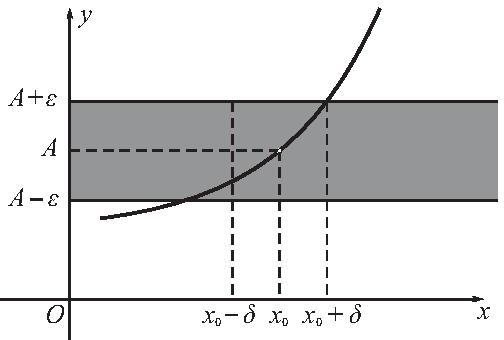
\includegraphics[scale=0.8]{pic/C-1/极限1.pdf}
	\end{center}
	\vspace*{-1em} \vspace*{-1em} 
	\caption{极限的定义图解}
\end{figure}
\vspace*{-1em}

\subsection{自变量趋于无穷大时函数的极限}
\vspace*{-1em}

\defination[函数极限2]
设函数$f(x)$在当$|x|$大于某一正数时恒有定义.如果存在常数$A$,对于任意给定的正数$\varepsilon$(不论它多么小),总存在正数$X$使得当$x$满足不等式$|x|>X$时,对应的函数值$f(x)$都满足不等式
\begin{equation}
	|f(x)-A|<\varepsilon
\end{equation}
那么常数$A$就叫做函数$f(x)$当$x \to x_0$的\dy[极限]{JX},记作
\begin{equation}
	\lim\limits_{x\to \infty}f(x)=A \quad \mbox{或} \quad f(x)\to A(x \to \infty )
\end{equation}

\subsection{无穷小与无穷大}
\vspace*{-1em}

\defination[无穷小]
如果函数$f(x)$当$x\to x_0\left(\mbox{或}x \to \infty  \right) $时的极限为$0$,那么称函数$f(x)$为当$x\to x_0\left(\mbox{或}x \to \infty  \right) $时的\dy[无穷小]{WQX}.记为
\begin{equation}
	\lim\limits_{x \to x_0}f(x)=0,\lim\limits_{x\to \infty}f(x)=0.
\end{equation}
特别地,以$0$为极限的数列${x_n}$称为$n\to \infty$时的\dy[无穷小]{WQX}.
\vspace*{1em}

\defination[无穷大]
设函数$f(x)$在$x_0$的某一去心邻域内有定义(或$|x|$趋于某一正数时有定义).如果对于任意给定的正数$M$(不论它多么大),总存在正数$\delta$(或正数$X$),只要$x$适合不等式$0<|x-x_0|<\delta$(或$|x|>X$),对应函数值$f(x)$总满足不等式
\begin{equation*}
	|f(x)|>M
\end{equation*}
那么称函数$f(x)$为当$x\to x_0\left(\mbox{或}x \to \infty  \right) $时的\dy[无穷大]{WQD}.记为
\begin{equation}
	\lim\limits_{x \to x_0}f(x)=\infty,\lim\limits_{x\to \infty}f(x)=\infty.
\end{equation}

\subsection{单侧极限}
\vspace*{-1em}

\defination[左极限]
在 $\lim\limits_{x \to x_0}f(x)=A$的定义中,把$0<|x-x_0 |<\delta$改为$x_0-\delta <x<x_0$ ,那么$A$就叫做函数$f(x)$当$x \to x_0$时的\dy[左极限]{ZJX}.记作
\begin{equation}
	\lim\limits_{x \to x_0^-}f(x)=A \quad \mbox{或} \quad f(x_0^-)=A \quad \mbox{或} \quad \lim\limits_{x \to x_0 - 0}f(x)=A
\end{equation}

\defination[右极限]
在 $\lim\limits_{x \to x_0}f(x)=A$的定义中,把$0<|x-x_0 |<\delta$改为$x_0 <x<x_0+\delta$ ,那么$A$就叫做函数$f(x)$当$x \to x_0$时的\dy[右极限]{YJX}.记作
\begin{equation}
	\lim\limits_{x \to x_0^+}f(x)=A \quad \mbox{或} \quad f(x_0^+)=A \quad \mbox{或} \quad \lim\limits_{x \to x_0 + 0}f(x)=A
\end{equation}

\subsection{利用定义求函数的极限的解题方法}
\vspace*{-1em}

\example[可以直接求得$\delta$与$\varepsilon$的关系]
任意一个$\varepsilon$满足$|f(x)-A|<\varepsilon$,都能找到一个正数$\delta$使$0 < |x - x_0| < \delta$或$|x| > \delta$ ,这就说明了$\varepsilon$与$\delta $有个对应关系,即
\begin{equation}
	\delta=\varphi(\varepsilon)
\end{equation}
\par $\delta=\varphi(\varepsilon)$这个关于$\varepsilon$的函数可以是任意的.所以我们利用极限的定义来证明某个函数的极限时,只需找到$\varepsilon$和$\delta$之间的对应关系.这时,我们可以先利用$|f(x)-A|<\varepsilon$这个条件,然后构造出 $|x - x_0| < \varphi(\varepsilon)$的形式即可.(对于求数列的极限时$\delta$换成$N$即可.)

\examples 证明下列极限\\[0.5em]
\hspace*{0.8em} $1.\,\,\lim\limits_{x \to 3}2x-1=5$

\proof  设$\exists \delta,\forall \varepsilon$,当$0<|x-3|<\delta $时,$|2x-1-5|=|2x-6|=2|x-3|<\varepsilon$\quad \quad 【构造$|x-x_0 | < \varphi (\varepsilon)$】\\[0.5em]
即$\displaystyle |x-3|<\frac{\varepsilon}{2}$,故取$\displaystyle \delta = \frac{\varepsilon}{2}$时成立,证毕.\\[1.5em]
\hspace*{0.8em} $2.\,\,\displaystyle \lim\limits_{x \to \infty }\frac{1}{x}=0$\\[1em]
\proof  设$\exists N,\forall \varepsilon$,当$|x|>N$时,$\displaystyle \left| \frac{1}{x}-0\right| =\left| \frac{1}{x}\right|<\varepsilon$\hspace{13em}【构造$|x-x_0 | < \varphi (\varepsilon)$】\\[0.5em]
即$\displaystyle |x|>\frac{1}{\varepsilon}$,故取$\displaystyle N = \frac{1}{\varepsilon}$时成立,证毕.\\

\example[不能直接求得$\delta$与$\varepsilon$的关系]
\noindent 【方法一】放缩法\vspace{0.3em}
\par 这个时候我们可以将$|f (x) - A|$进行适当的放大,使得$\delta $与$\varepsilon$的关系容易求得,一般的放缩方法有:\\[0.5em]
\noindent (1) 将分母恒大于零的部分(可以含$x$)删去;\\[0.5em]
\noindent (2) 将分子恒小于零的部分删去(可以含$x$);\\[0.5em]
\noindent (3) 将幂函数的底数部分进行放缩.

\examples 证明$\displaystyle \lim\limits_{x \to 1}\sqrt{3x+1}=2.$

\proof 设$\exists \delta,\forall \varepsilon$,当$0<|x-1|<\delta $时,$\displaystyle |\sqrt{3x+1}-2|=\frac{3(x-1)}{\sqrt{3x+1}+2}\le \frac{3}{2}|x-1|<\varepsilon$\hspace{4em}【放缩构造】\\[0.5em]
即$\displaystyle |x-1|<\frac{2}{3}\varepsilon$,又$\displaystyle \sqrt{3x+1}$定义域为$\displaystyle x>-\frac{1}{3}$,那么$\displaystyle x-1>-\frac{4}{3}$,在一定范围内有$\displaystyle |x-1|<\frac{4}{3}$\hspace{1em}【判断定义域】\\[0.5em]
故取$\displaystyle \delta = \min \left\lbrace  \frac{2}{3}\varepsilon,\frac{4}{3} \right\rbrace $时成立,证毕.\hspace{27em}【取最小值】\\

\noindent 【方法二】先设后求再取值法\vspace{0.8em}
\par 放缩不是唯一的方法,我们还可以先设后求再取$\delta $最小值.\\[0.3em]
\noindent (1) 先化简式子,且含$|x-a|$项,这个时候可以用该方法;\\[0.5em]
\noindent (2) 设$\delta $的值为$f(a)$ (可以含$a,x$,也可以是常数);\\[0.5em]
\noindent (3) 解出$x$的范围,对非$|x - a|$的项进行放缩,将式子放大,同时使得非$|x - a|$的项转换为常量;\\[0.5em]
\noindent (4) 反解出$\delta = \varphi (\varepsilon)$;\\[0.5em]
\noindent (5) 取$\delta = \min \lbrace f(a),\varphi(\varepsilon)\rbrace$.\vspace{0.5em}
\par 当然通常放缩法和先设后求再取值法会结合用,这样就可以解决大部分题目.
\par 但是在后面的证明过程中,一般简单的函数极限可以直接用,所以一般情况下不会用定义证明极限.

\examples 证明$\lim\limits_{x \to a}x^2=a^2$

\proof 由于$|x^2-a^2|=|(x-a)(x+a)|=|x-a|\cdot |x+a| $,\hspace{16em}【找到$|x-a|$项】\\[0.5em]
设$\displaystyle |x-a|<\frac{1}{2}$,则$\displaystyle |x+a|=|x-a+2a|\le |x-a|+|2a|<\frac{1}{2}+|2a|.$ \hspace*{2em}【赋值$|x-a|$项,并放缩得出未知项的范围】\\[0.5em]
所以,设$\exists \delta,\forall \varepsilon$,当$0<|x-1|<\delta $时,$\displaystyle |x^2-a^2|=|x-a|\cdot |x+a|<\left( \frac{1}{2}+|2a|\right)|x-a|<\varepsilon $,\\[0.5em]
即$\displaystyle|x-a|<\frac{\varepsilon}{\frac{1}{2}+2|a|}$.\hspace{29em}【反解出$|x-a|$的范围】\\[0.5em]
故取$\displaystyle \delta = \min \left\lbrace  \frac{\varepsilon}{\frac{1}{2}+2|a|},\frac{1}{2} \right\rbrace $时成立,证毕.\hspace{26em}【取最小值】

\subsection{证明函数的极限不存在的方法}
\vspace*{-1em}

\theorem[序列极限]
设函数$f (x)$在$a$点的一个空心邻域内有定义,并且$\lim\limits_{x \to a}f(x)=l$.假若是一串在该空心邻域内取值的序列,且
\begin{equation*}
	\lim\limits_{n \to \infty}x_n=a
\end{equation*}
则有
\begin{equation}
	\lim\limits_{n \to \infty}f(x_n)=l
\end{equation}
\par 这个定理为我们提供了一种\textbf{证明函数极限不存在的办法}:对于一个定义在$a$点的某空心邻域内的函数$f(x)$,如果能找到两串序列$\lbrace x'_n \rbrace $与$\lbrace x''_n\rbrace$它们都在$a$的该空心邻域内取值,且当$n\to \infty $时都以$a$为极限,而极限$\lim\limits_{n \to \infty }x'_n$与 $\lim\limits_{n \to \infty }x''_n$都存在但不相等,则$f(x)$在$x \to a$时不可能有极限.\vspace*{1em}

\example[证明函数的极限不存在]
\vspace*{-1em} \examples 证明:函数$\displaystyle \sin \frac{1}{x}$在$x\to 0$时没有极限.

\proof 取$\displaystyle x'_n=\frac{1}{2n\pi }$,则$\displaystyle \sin \frac{1}{x'_n}=0$;而取$\displaystyle x''_n=\frac{1}{2n\pi+\frac{\pi}{2} }$,则$\displaystyle \sin \frac{1}{x'_n}=1.$\\[0.5em]
这时由于$n \to \infty \Rightarrow x'_n\to 0,x''_n \to 0, $且
\begin{equation*}
	\lim\limits_{n \to \infty} \sin \frac{1}{x'_n} \ne \lim\limits_{n \to \infty} \sin \frac{1}{x''_n} 
\end{equation*}
因此,函数$\displaystyle \sin \frac{1}{x}$在$x\to 0$时没有极限.

\section{利用极限运算法则和两个准则求极限}
\subsection{极限运算法则}
\vspace*{-1em}

\theorem[极限运算法则1]
两个无穷小的和是无穷小.

\tl 有限个无穷小的和是无穷小.
\newpage
\theorem[极限运算法则2]
有界函数与无穷小的乘积是无穷小.

\tl 常数与无穷小的乘积是无穷小.

\tl 有限个无穷小的乘积是无穷小.\vspace*{1em}

\theorem[极限运算法则3]
如果$\lim f(x) = A, \lim g(x) = B$(这些函数都必须存在极限),那么
\begin{equation}
	\lim [f(x)\pm g(x)]=\lim f(x)\pm \lim g(x)=A \pm B
\end{equation}
\begin{equation}
	\lim[f(x)\cdot g(x)]=\lim f(x)\cdot \lim g(x)=A\cdot B
\end{equation}
若$B\ne 0$,那么
\begin{equation}
	\lim \left[ \frac{f(x)}{g(x)}\right] =\frac{\lim f(x)}{\lim g(x)}=\frac{A}{B}
\end{equation}

\tl 如果$\lim f(x)$存在,而$c$为常数,那么
\begin{equation}
	\lim [cf(x)]=c \lim f(x)
\end{equation}

\tl 如果$\lim f(x)$存在而$n$为正整数,那么
\begin{equation}
	\lim [f(x)]^n=[\lim f(x)]^n
\end{equation}

\theorem[极限运算法则4]
如果$\varphi(x) \ge \psi(x),$而$\lim \varphi(x)=A,\lim \psi(x)=B,$则$A \ge B.$\vspace*{1em}

\subsection{极限运算准则}
\vspace*{-1em}

\theorem[单调有界数列极限一定存在]
(1)  \quad 若$x_{n+1} \le x_n(n\mbox{为正整数})$,且$x_n \ge m,$则$\lim\limits_{n \to \infty }x_n = A $存在,且$A \ge m$;
\par (2)  \quad 若$x_{n+1} \ge x_n(n\mbox{为正整数})$,且$x_n \le M,$则$\lim\limits_{n \to \infty }x_n = A $存在,且$A \le M$.

\theorem[夹逼定理]
设$g(x) \le f(x) \le h(x)$,若$\lim\limits_{x \to m}g(x)=A,\lim\limits_{x \to m}=A,(-\infty \le m \le +\infty)$则$\lim\limits_{x \to m}f(x)=A.$\vspace*{1em}

\subsection{例题}
\vspace*{-1em}

\example[利用极限运算法则和两个准则求极限]\vspace*{-1em}
\examples 证明:$\lim\limits_{n \to \infty}q^n=0.(|q|<1)$

\proof 设$\displaystyle |q|=\frac{1}{1+a},a>0,$则$\displaystyle 0< q^n=\frac{1}{(1+a)^n}=\frac{1}{C^0_na^0=C^1_na^1+C^2_na^2+\cdots+C^n_na^n}<\frac{1}{C^1_na^1}=\frac{1}{na}.$\\[0.5em]
又$\displaystyle \lim\limits_{n \to \infty}\frac{1}{na}=0,\lim\limits_{n\to \infty}0=0,$由夹逼定理可得
\begin{equation*}
	\lim\limits_{n\to \infty}0 \le \lim\limits_{n \to \infty}q^n \le \lim\limits_{n \to \infty}\frac{1}{na}
\end{equation*}
故$\lim\limits_{n \to \infty}q^n=0.$\vspace*{1em}

\examples 证明:$\displaystyle a_n=\frac{a^n}{n!}(a\mbox{是大于1的任意常数})$存在极限.

\proof 当$n>[a]+1$时,有
\begin{equation*}
	0\le a_n =\frac{a^{[a]}}{[a]!}\cdot \frac{a}{[a]+1}\cdot \frac{a}{[a]+2}\cdot \,\,\cdots \,\,\cdot \frac{a}{n}<\frac{a^{[a]}}{[a]!}\cdot \frac{a}{n}
\end{equation*}
注意到$\displaystyle \frac{a^{[a]}}{[a]!}$是一个常数,所以$\displaystyle \lim\limits_{n \to \infty}\frac{a^{[a]}}{[a]!}\cdot \frac{a}{n}=0,$由夹逼定理可得
\begin{equation*}
	\lim\limits_{n \to \infty}a_n=0.
\end{equation*}

\examples 设常数$a>1,$对于任意自然数$k$,证明:
\begin{equation*}
	\lim\limits_{n \to \infty}\frac{n^k}{a^n}=0.
\end{equation*}
\hspace*{-0.5em}\proof 令$t=a-1$,则$t>0$,那么
\[
a_n=(1+t)^n=1+nt+\frac{n(n-1)}{2!}t^2+\cdots+\frac{n(n-1)\cdot(n-k)}{(k+1)!}t^{k+1}+\cdots+t^n,
\]
因此,当$n>1$时,$\displaystyle a^n>\frac{n(n-1)\cdots(n-k)}{(k+1)!}t^{k+1}$,于是
\[
0 \le \frac{n^k}{a^n}\le \frac{n^k}{\displaystyle \frac{n(n-1)\cdots(n-k)}{(k+1)!}t^{k+1}}=\frac{(k+1)!}{t^{k+1}}\cdot \frac{n^k}{n(n-1)\cdots(n-k)}=\frac{(k+1)!}{t^{k+1}}\cdot\frac{n^k}{\lambda_{k+1}n^{k+1}+\lambda_kn^k+\cdots+\lambda_1n+\lambda_0}
\]
其中$\lambda_0,\lambda_1,\cdots,\lambda_{k+1}$均为非零常数.注意到$\displaystyle \frac{(k+1)!}{t^{k+1}}$为常数,则
\begin{equation*}
	\begin{split}
		&\quad \, \lim\limits_{n \to \infty}\frac{(k+1)!}{t^{k+1}}\cdot\frac{n^k}{\lambda_{k+1}n^{k+1}+\lambda_kn^k+\cdots+\lambda_1n+\lambda_0}\\
		&=\lim\limits_{n \to \infty}\frac{(k+1)!}{t^{k+1}}\cdot\frac{1}{n}\cdot \frac{n^k}{\lambda_{k+1}+\lambda_kn^{-1}+\cdots+\lambda_1n^{-k}+\lambda_0n^{-k-1}}=0
	\end{split}
\end{equation*}
因此,由夹逼定理可得
\begin{equation*}
	\lim\limits_{n \to \infty}\frac{n^k}{a^n}=0.
\end{equation*}

\section{利用等价无穷小求极限}
\subsection{无穷小的分类}
\vspace*{-1em}

\defination[无穷小的分类]
设$\alpha,\beta $是同一变化过程中的无穷小,$\displaystyle \lim \frac{\beta}{\alpha}$是这一过程的极限,$c$为常数,那么\\[0.5em]
\noindent (1) \quad $\displaystyle \lim \frac{\beta }{\alpha}=0$,则称$\beta $是$\alpha $的\dy[高阶无穷小]{GJWQX},记作$\beta = o(\alpha)$.\\[0.5em]
\noindent (2) \quad  $\displaystyle \lim \frac{\beta }{\alpha}=\infty$,则称$\beta $是$\alpha $的\dy[低阶无穷小]{DJWQX1}.\\[0.5em]
\noindent (3) \quad  $\displaystyle \lim \frac{\beta }{\alpha}=c \ne 0$,则称$\beta $是$\alpha $的\dy[同阶无穷小]{TJWQX}.\\[0.5em]
\noindent (4) \quad  $\displaystyle \lim \frac{\beta }{\alpha}=1$,则称$\beta $是$\alpha $的\dy[等价无穷小]{DJWQX2},记作$\beta \sim \alpha$.\\[0.5em]
\noindent (3) \quad  $\displaystyle \lim \frac{\beta }{\alpha^k}=c \ne 0$,则称$\beta $是$\alpha $的\dy[$k$阶无穷小]{KJWQX}.

\warn[
{\large \bf 0与``0"的区别}\vspace*{0.5em}\\
\hspace*{1em}(1)\quad ``0"指的是无穷小,设$\alpha$是某一变化过程中的无穷小,也就是说$x$趋于某一值时,极限为0.\vspace*{0.5em}\\
\hspace*{1em}(2)\quad 当0指的是实数0时,$\lim 0 \cdot f(x)=0$,这与$f(x)$无关,即使$\lim f(x)=\infty$,其结果仍然是0,因为0在这里是实数,而不是无穷小.
]


\subsection{常见的等价无穷小}
\vspace*{-1em}

\theorem[常见的等价无穷小]
以下等价无穷小均为$x \to 0$这一变化过程,其中$x$也可替换为一个函数,即$f(x) \to 0$的情况也适用.
\begin{equation}
	\tan x \sim \sin x \sim x \sim \arcsin x \sim \arctan x
\end{equation}
\begin{equation}
	\ln (1+x) \sim x
\end{equation}
\begin{equation}
	x \sim \e^x -1
\end{equation}
\begin{equation}
	1-\cos x \sim \frac{x^2}{2}
\end{equation}
\begin{equation}
	\sec x -1 =\frac{1}{\cos x}-1 \sim \frac{x^2}{2}
\end{equation}
\begin{equation}
	(1+x)^a-1 \sim ax
\end{equation}
\begin{equation}
	a^x-1 \sim \ln a \cdot x \,(a>0,a \ne 1)
\end{equation}
\subsection{等价无穷小求极限的本质}
等价无穷小求极限本质上是极限与1的相乘,而有等价无穷小的定义,1可以换成极限$\displaystyle 1=\lim\limits_{x \to x_0}\frac{\alpha }{\beta}$,再运用极限乘法运算法则计算即可.

\example[等价无穷小的误用]\vspace*{-1em}
\examples \label{例 1.8}求极限$\displaystyle \lim\limits_{x \to 0}\frac{\tan x -\sin x}{\sin^3 x}$.

\errsolve  由于$\tan \sim \sin x \sim x$得$\displaystyle \lim\limits_{x \to 0}\frac{\tan x -\sin x}{\sin^3 x}=\lim\limits_{x \to 0}\frac{x-x}{\sin^3 x}=\lim\limits_{x \to 0}0=0.$

\errreason  在运用等价无穷小的时候没有考虑极限运算法则成立的条件.

\solvereason $\displaystyle \lim\limits_{x \to 0}\frac{\tan x -\sin x}{\sin^3 x}=\lim\limits_{x \to 0}\frac{\tan x}{\sin^3 x} - \lim\limits_{x \to 0}\frac{\sin x}{\sin^3 x}$实际上运用了法则$\lim [f(x)-g(x)]=\lim f(x)-\lim g(x),$\\[1em]即完整的错解解题步骤应为
\begin{equation*}
	\lim\limits_{x \to 0}\frac{\tan x -\sin x}{\sin^3 x}=\lim\limits_{x \to 0}\frac{\tan x}{\sin^3 x} - \lim\limits_{x \to 0}\frac{\sin x}{\sin^3 x}
	=\lim\limits_{x \to 0}\frac{\tan x}{\sin^3 x}\cdot \lim\limits_{x \to 0} \frac{x}{\tan x}-\lim\limits_{x \to 0}\frac{x}{\sin^3 x}
\end{equation*}
而极限运算法则成立的条件是$\lim f(x),\lim g(x)$存在,而$\displaystyle \lim\limits_{x \to 0}\frac{\tan x}{\sin^3 x}$不存在,因此解题错误.

\solve $\displaystyle \lim\limits_{x \to 0}\frac{\tan x -\sin x}{\sin^3 x}=\lim\limits_{x \to 0}\frac{\sin x(\sec x-1)}{\sin^3 x}=\lim\limits_{x \to 0}\frac{\sec x-1}{\sin^2 x} \cdot \lim\limits_{x \to 0}\frac{\frac{x^2}{2}}{\sec x -1} \cdot \lim\limits_{x \to 0}\frac{\sin x^2}{x^2}
=\frac{\frac{x^2}{2}}{x^2}=\frac{1}{2}.$\vspace*{1em}

\examples 求极限$\displaystyle \lim_{x \to 0} \frac{\sin \left(x^2 \sin{\frac{1}{x}}\right) }{x}.$

\errsolve $\displaystyle \lim_{x \to 0}\frac{\sin \left(x^2 \sin{\frac{1}{x}}\right) }{x}=\lim_{x \to 0}\frac{x^2 \sin \frac{1}{x}}{x}=\lim_{x \to 0}x\sin\frac{1}{x}=0.$

\errreason 对极限概念的理解不清晰,不仔细,没有严格判断等价无穷小的定义式是否满足极限的定义.

\solvereason 实际上,该错误解答的完整版本应该为:
\[
\lim_{x \to 0} \frac{\sin \left(x^2 \sin{\frac{1}{x}}\right) }{x}=\lim_{x \to 0} \frac{\sin \left(x^2 \sin{\frac{1}{x}}\right) }{x}\cdot\frac{x^2\sin \frac{1}{x}}{\sin \left( x^2 \sin \frac{1}{x}\right) }=\lim_{x \to 0}\frac{x^2\sin\frac{1}{x}}{x}=\lim_{x \to 0}x\sin \frac{1}{x}=0.
\]
但是极限
\[
\lim_{x \to 0}\frac{x^2\sin \frac{1}{x}}{\sin \left( x^2\sin \frac{1}{x}\right) }
\]
中,若$\displaystyle \sin \frac{1}{x}$取0,则这个极限式无意义(分母为0).故$\displaystyle x \ne \frac{1}{k \pi}(k \in Z).$\hspace*{12.5em}【判断定义域】\\[0.5em]
\hspace*{2em}这样的话,在点$x = 0$的任何一个去心邻域中都有无穷多个点没有定义,所以不存在一个去心邻域满足该极限式,
故极限不存在.\hspace*{24em}【判断是否能找到满足的去心邻域】\\[0.5em]
这里再次强调一下0与``0"的区别: 分母为0的时候并不是指无穷小量,而是真正意义上的0.

\solve 设$\exists \delta, \forall \varepsilon,$使得当$|x-0|<\delta$时,$\displaystyle \left| \frac{\sin \left( x^2\sin\frac{1}{x}\right) }{x}-0\right|<\varepsilon$,\\[0.5em]
由不等式$|\sin x|\le |x|$,得
\[
\left| \frac{\sin \left( x^2\sin\frac{1}{x}\right) }{x}\right| \le \left| \frac{ \left( x^2\sin\frac{1}{x}\right) }{x}\right| =\left| x \sin \frac{1}{x} \right|.
\]
由$\displaystyle \left| \sin \frac{1}{x} \right| \le 1$,得
\[
\left| \frac{\sin \left( x^2\sin\frac{1}{x}\right) }{x}\right| \le \left| \frac{ \left( x^2\sin\frac{1}{x}\right) }{x}\right| =\left| x \sin \frac{1}{x} \right|.\le |x|<\varepsilon
\]

\subsection{例题}
\vspace*{-1em}
\example[等价无穷小的运用]
在下面的例题中,为了方便,省略了含有等价无穷小本质的式子.但是建议读者在实际做题的过程中还是要写完整,方便利用定义检查式子的合理性.

\examples 求极限$\displaystyle \lim_{x \to \infty}\left(\cos \frac{3}{x} \right)^{x^2} $

\solve 令$\displaystyle t=\frac{1}{x}$,则$x=\dfrac{1}{t},x\to \infty ,t \to 0.$

\newpage 
\vspace*{-2em}
\[
\lim_{x \to \infty}\left(\cos \frac{3}{x} \right)^{x^2} =\lim_{t \to 0}(\cos 3t)^{\frac{1}{t^2}}=\lim_{t \to 0}\left[\left( 1-2\sin^2\frac{3t}{2}\right)^{\frac{1}{2\sin^2\frac{3t}{2}}} \right]^{\frac{2\sin^2\frac{3t}{2}}{t^2}} =\e^{\displaystyle -\lim_{t \to 0}\frac{2\sin^2\frac{3t}{2}}{t^2}}
\]
因为$\displaystyle \lim_{t \to 0}\frac{2\left( \displaystyle \frac{3t}{2}\right)^2 }{t^2}=\frac{9}{2},\,\therefore \lim_{x \to \infty }\left(\cos \frac{3}{x} \right)^{x^2}=\e^{ \displaystyle  -\lim_{t \to 0}\frac{2\sin^2\frac{3t}{2}}{t^2}}=\e ^{-\frac{9}{2}} $

\solveother 令$\displaystyle t=\frac{1}{x}$,则$\displaystyle x=\frac{1}{t},x\to \infty ,t \to 0.$
\[
\lim_{x \to \infty}\left( \cos \frac{3}{x}\right)^{x^2} =\lim_{t \to 0}(\cos 3t)^{\frac{1}{t^2}}=\e^{\lim\limits_{t \to 0}\ln(\cos 3t)^{\frac{1}{t^2}}}
\]
\[
\because \lim\limits_{t \to 0}\frac{1}{t^2}\ln(\cos 3t)=\lim\limits_{t \to 0}\frac{1}{t^2}\ln (\cos 3t)=\lim\limits_{t \to 0}\frac{1}{t^2}\ln \left[1+\left(-2\sin^2\frac{3t}{2}\right)\right]=\lim_{t \to 0}\frac{-2\sin^2\frac{3t}{2}}{t^2}=\lim\limits_{t \to 0}\frac{-2\left(\frac{3t}{2}\right)^2}{t^2}=-\frac{9}{2}.
\]
\[
\therefore \lim_{x \to \infty}\left( \cos \frac{3}{x}\right)^{x^2}=\lim\limits_{t \to 0}(\cos 3t)^{\frac{1}{t^2}}=\e^{\lim\limits_{t \to 0}\ln(\cos 3t)^{\frac{1}{t^2}}}=\e^{-\frac{9}{2}}.
\]

\inference[等价无穷小类型\uppercase\expandafter{\romannumeral1}]
以上是利用两种等价无穷小的解法,下面对这两种等价无穷小的用法归类.(这两个极限选一个用即可).若一个极限表达式有下列的形式(或者经过换元、取对数等方法变成这种形式),则很有可能用到这两种极限.
\begin{equation}
	\lim f(x)^{g(x)}
\end{equation}
其中$\lim f(x)=1,\lim g(x)$存在.

解法一\qquad 变形为:
\begin{equation}
	\lim\big[1+\big(f(x)-1\big)\big]^{g(x)}=\lim\big[1+\big(f(x)-1\big)\big]^{\frac{g(x)[f(x)-1]}{f(x)-1}}=\e^{\lim g(x)\cdot [f(x)-1]}
\end{equation}
而此时$\lim g(x) \cdot [f(x)-1]$是容易求得的.


解法二\qquad 变形为:
\begin{equation}
	\lim\big[1+\big(f(x)-1\big)\big]^{g(x)}=\e^{\lim \ln[1+\left( f(x)-1\right) ]}=\e^{\lim g(x)\cdot [f(x)-1]}
\end{equation}
而此时$\lim g(x) \cdot [f(x)-1]$也是容易求得的.

\examples 已知函数$f(x)$满足$\displaystyle \lim_{x \to 0}\frac{\sqrt{1+f(x)\sin 2x}-1}{\e^{3x}-1}=2$,求$\displaystyle \lim_{x \to 0}f(x).$

\solve $\displaystyle \lim_{x \to 0}\frac{\sqrt{1+f(x)\sin 2x}-1}{\e^{3x}-1}=\lim\limits_{x \to 0}\frac{1/2f(x)\sin 2x}{3x}=\lim_{x \to 0}\frac{1/2f(x)2x}{3x}=\frac{1}{3}\lim_{x\to 0}f(x)=2.$
\[
\therefore \lim_{x \to 0}f(x)=6.
\]

下面给出一个较难看出错误的例题.

\examples \label{例 1.12}求极限$\displaystyle \lim_{x \to 0}\left[ \frac{(1+x)^{\frac{1}{x}}}{\e}\right]^{\frac{1}{x}}.$

\errsolve $\displaystyle \lim_{x \to 0}\left[ \frac{(1+x)^{\frac{1}{x}}}{\e}\right]^{\frac{1}{x}}=\lim_{x \to 0}\left[ \frac{\e}{\e}\right]^{\frac{1}{x}}=1.$

\errreason 在运用等价无穷小的时候没有考虑极限运算法则成立的条件.

\solvereason $\displaystyle \lim_{x \to 0}\left[ \frac{(1+x)^{\frac{1}{x}}}{\e}\right]^{\frac{1}{x}}=\e^{\lim\limits_{x \to 0}\frac{1}{x}\ln\frac{(1+x)^{\frac{1}{x}}}{\e}},$
\[
\lim_{x \to 0}\frac{1}{x}\ln\frac{(1+x)^{\frac{1}{x}}}{\e}=\lim\limits_{x \to 0}\frac{1}{x}\left[ \ln(1+x)^{\frac{1}{x}} -\ln \e\right]=\lim\limits_{x \to 0}\frac{1}{x}\cdot\lim\limits_{x \to 0}\left[ \ln(1+x)^{\frac{1}{x}} -\ln \e\right]=\lim_{x \to 0}\frac{1}{x} \cdot \lim\limits_{x \to 0} \left[ \ln \e -\ln \e \right]=0.
\]
实际上,在$\displaystyle \lim\limits_{x \to 0}\frac{1}{x}\left[ \ln(1+x)^{\frac{1}{x}}-\ln \e \right]=\lim\limits_{x \to 0}\frac{1}{x}\cdot\lim\limits_{x \to 0}\left[ \ln(1+x)^{\frac{1}{x}} -\ln \e\right]$中用到了$\lim \big[f(x)\cdot g(x)\big]=\lim f(x) \cdot \lim  g(x)$,即用到了极限运算法则,而$\displaystyle \lim_{x \to 0}\frac{1}{x}$不存在,因此这种运算错误.

\solve $\displaystyle \lim_{x \to 0}\left[ \frac{(1+x)^{\frac{1}{x}}}{\e}\right]^{\frac{1}{x}}=\lim_{x \to 0}\left\lbrace1+\left[\frac{(1+x)^{\frac{1}{x}}}{\e}-1\right]\right\rbrace^{\frac 1x}=\lim_{x \to 0}\left\lbrace1+\left[\frac{(1+x)^{\frac{1}{x}}}{\e}-1\right]\right\rbrace^{ \frac{1}{(1+x)^{\frac 1x}-1}\cdot \frac{(1+x)^{\frac 1x}-1}{x}},$
\[
\because \lim\limits_{x \to 0}\left[\frac{(1+x)^{\frac{1}{x}}}{\e}-1\right]=0,\therefore \lim_{x \to 0}\left\lbrace1+\left[\frac{(1+x)^{\frac{1}{x}}}{\e}-1\right]\right\rbrace^{ \frac{1}{(1+x)^{\frac 1x}-1}\cdot \frac{(1+x)^{\frac 1x}-1}{x}}=\e^{\lim\limits_{x\to 0}\frac{(1+x)^\frac 1x-1}{x}},
\]
\[
\because \lim\limits_{x\to 0}\frac{\frac{(1+x)^\frac 1x}{\e}-1}{x}=\lim\limits_{x\to 0}\frac{(1+x)^\frac 1x-\e}{\e x}=\lim\limits_{x \to 0}\frac{\e^{\frac{1}{x}\ln(1+x)}-\e}{\e x}\xlongequal[]{\e^x-1 \sim x} \lim\limits_{x \to 0}\frac{\frac{1}{x}\ln(1+x)-1}{x}=\lim_{x \to 0}\frac{\ln (1+x)-x}{x^2}
\]
\[
\xlongequal[]{\ln(1+x)-x\sim-\frac{1}{2}x^2} \lim\limits_{x \to 0}\frac{-\frac{1}{2}x^2}{x^2}=-\frac{1}{2}
\]
\[
\therefore \lim_{x \to 0}\left[ \frac{(1+x)^{\frac{1}{x}}}{\e}\right]^{\frac{1}{x}}=\e^{\lim\limits_{x\to 0}\frac{(1+x)^\frac 1x-1}{x}}=\e^{-\frac{1}{2}}=\frac{\sqrt{\e}}{\e}.
\]

\inference[等价无穷小求极限]\vspace*{-1em}
\begin{enumerate}
	\item 判断并构造等价无穷小的类型(7 种);
	\item 利用等价无穷小求极限的本质列出计算式;
	\item 判断等价无穷小的极限式中能否找到满足定义域的去心邻域使得极限存在:
	\begin{enumerate}[(i)]
		\item 若存在,则利用等价无穷小解题;
		\item 若不存在,则用其它方法求解(如利用函数定义、夹逼准则等).
	\end{enumerate}
	\item 检验计算的每一步是否都符合极限运算法则的前提条件.
\end{enumerate}
\vspace*{-2em}
\warn[
\hspace*{2em}1. 以上等价无穷小都只在$x\to 0$的情况下才成立,$x$趋于其它值时不成立.\\
\hspace*{2em}2. 只有等价无穷小的定义式存在极限的前提下,即在函数$f (x)$的定义域内能找到一个完整的去心邻域,$x$才可以用任意函数$f(x)$替换.若等价无穷小的定义式都不存在极限,又谈何等价无穷小.\\
下面给出常见的一些不可以用等价无穷小替换的函数.\vspace*{1em}\\
\examples $\displaystyle x \to 0,\sin\left(x \sin \frac 1x\right) \not \sim x\sin \frac{1}{x},\sin\left(x\cos \frac 1x\right)\not \sim x \cos \frac 1x$\\
\hspace*{2em}3. 在运用等价无穷小计算极限的时候要特别要注意在替换的过程中只有符合极限的运算法则,才可以进行
替换(通常极限的运算法则不明显,需要仔细计算),前面已经给出了两个详细的例子.
]

\section{函数连续性}
\subsection{函数连续性的定义}
\vspace*{-1em}

\defination[函数在某点的连续性\uppercase\expandafter{\romannumeral1}]
设函数$y=f(x)$在点$x_0$的某一邻域内有定义,如果
\begin{equation}
	\lim\limits_{\Delta x \to 0}\Delta y=\lim\limits_{\Delta x \to 0}\big[f(x_0+\Delta x)-f(x_0)\big]=0.
\end{equation}
那么就称函数$y=f(x)$在点$x_0$处\dy[连续]{LX}.

\defination[函数在某点的连续性\uppercase\expandafter{\romannumeral2}]
设函数$y=f(x)$在点$x_0$的某一邻域内有定义,如果
\begin{equation}
	\lim\limits_{x \to x_0} f(x)=f(x_0).
\end{equation}
那么就称函数$y=f(x)$在点$x_0$处\dy[连续]{LX}.\vspace*{1em}

即$f(x)$在点$x_0$处连续$\Longleftrightarrow \forall \varepsilon>0,\exists \delta>0,$当$|x-x_0|<\delta$时,都有$|f(x)-f(x_0)|<\varepsilon$

\defination[左连续]
如果$\lim\limits_{x \to x_0^-}f(x)=f(x_0^-)$存在且等于$f(x_0)$,即$f(x_0^-)=f(x_0)$,那么就称函数$y=f(x)$在点$x_0$处\dy[左连续]{ZLX}.

\defination[右连续]
如果$\lim\limits_{x \to x_0^+}f(x)=f(x_0^+)$存在且等于$f(x_0)$,即$f(x_0^+)=f(x_0)$,那么就称函数$y=f(x)$在点$x_0$处\dy[右连续]{YLX}.

\warn[\hspace*{2em}函数在某点连续的充要条件是在该点的左极限和右极限都存在且都等于函数该点处的函数值.或者说函数在该点既左连续又右连续.(证明函数在某点处是否连续的方法)]


\defination[函数在某个区间的连续性]
在区间上每一点都连续的函数,叫做在该区间上的连续函数,或者说函数在该区间上连续.如果区间包括端点,那么函数在右端点是指右端点的左连续,在左端点是指左端点的右连续.

\textbf{连续函数的图形是一条连续而不间断的线(可能是直线,也可能是曲线).}

\subsection{函数的间断点}
\vspace*{-1em}

\defination[函数的间断点]
设函数$y=f(x)$在点$x_0$的某一邻域内有定义.在此前提条件下,如果函数有下列三种情况之一:\\[0.5em]
(1) 在$x=x_0$处没有定义;\hspace{12em}(2) 虽在$x=x_0$处有定义,但是$\displaystyle \lim\limits_{x \to x_0}f(x)$不存在;\\[0.5em]
(3) 虽在$x=x_0$处有定义,$\displaystyle \lim\limits_{x \to x_0}f(x)$存在,但$\displaystyle \lim_{x \to x_0}f(x) \ne f(x_0)$.\\[0.5em]
那么就称函数$f(x)$在点$x_0$处不连续,而点$x_0$称为函数$f(x)$的\dy[不连续点]{BLXD}或\dy[间断点]{JDD}.

如果$x_0$是函数$f(x)$的间断点,但左极限$f(x_0^-)$和右极限$f(x_0^+)$都存在,那么点$x_0$就称为函数$f(x)$的\dy[第一类间断点]{DYLJDD},不是第一类间断点的任何间断点都是\dy[第二类间断点]{DELJDD}.常见的具体分类见下表\ref{函数间断点的分类}.
\begin{table}[!htb]
	\centering
	\renewcommand{\arraystretch}{1}
	\setlength{\tabcolsep}{14mm}{
		\begin{tabular}{cc}
			\toprule[1.5pt] 
			第一类间断点 & 第二类间断点 \\
			\midrule
			可去间断点 & 无穷间断点\\
			跳跃间断点 & 震荡间断点\\
			\bottomrule[1.5pt]
		\end{tabular}  
	}
	\caption{函数间断点的分类}
	\renewcommand{\arraystretch}{1}
	\label{函数间断点的分类}
\end{table} 
\vspace*{-3em}

\defination[无穷间断点]
若$x_0$是函数$f(x)$的间断点,且$\lim\limits_{x \to x_0}f(x)=\infty $,那么我们称点$x_0$是函数的\dy[无穷间断点]{WQJDD}.\vspace*{1em}

\simpleexamples $\displaystyle x=\frac{\pi}{2}$是函数$y=\tan x$的无穷间断点.

\defination[振荡间断点]
若$x_0$是函数$f(x)$的间断点,且当$x \to x_0$时,函数值在多个值之间变动无穷多次,那么我们称点$x_0$是函数$f(x)$的\dy[振荡间断点]{ZDJDD}.\vspace*{1em}

\simpleexamples $\displaystyle x = 0$是函数$\displaystyle y =\sin\frac{1}{x}$的振荡间断点.
\warn[
\hspace*{2em} 若点$x_0$是函数$f(x)$的振荡间断点,那么在函数$f(x)$在点$x_0$处的任意的去心邻域都无确定的值.
进一步说,如果函数$f(x)$的导函数是$f'(x)$,点$x_0$是导函数$f'(x)$的振荡间断点,那么在$x_0$的任意去心邻域中函数$f(x)$的导数都不存在.
]
\vspace*{-1em}

\defination[可去间断点]
若点$x_0$是函数$f(x)$的间断点,且$f(x)$在点$x_0$处没有定义,而$\lim\limits_{x \to x_0}f(x)=f(x_0),$那么我们称点$x_0$是函数$f(x)$的\dy[可去间断点]{KQJDD}.\vspace*{1em}

\simpleexamples $\displaystyle x=1$是函数$\displaystyle y=\frac{x^2-1}{x-1}$的可去间断点.

\defination[跳跃间断点]
若点$x_0$是函数$f(x)$的间断点,且$f(x)$在点$x_0$处有定义,而$f(x_0^-)=f(x_0^+)$,那么我们称点$x_0$是函数$f(x)$的\dy[跳跃间断点]{TYJDD}.

\simpleexamples $\displaystyle x=0$是函数
$
\displaystyle
\begin{cases}
	x-1&,x<0\\
	0&,x=0\\
	x+1&,x>0
\end{cases}
$
的跳跃间断点.

\begin{tcolorbox}[sidebyside,colframe=red!75!black, colback=yellow!10!white,title=注意,sidebyside align=top seam,
	righthand width=4cm,fonttitle =\CJKfamily{heiti}]
	\hspace*{2em} 可去间断点的定义是左右极限相等即可,与函数在该点处是否有定义无关.关于这个很容易犯错,下面给出一个例子详细说明.
	\[
	f(x)=
	\begin{cases}
		x^2-1,&x<-3\\
		-1,&x=-3\\
		-3x-1,&-3<x\le 0
	\end{cases}
	\]
	如图,$\lim\limits_{x \to -3^-}f(x)=\lim\limits_{x \to -3^-}x^2-1=(-3)^2-1=8.$\\[0.5em]
	$\lim\limits_{x \to -3^+}=\lim\limits_{x \to -3^+}-3x-1=(-3)^2-1=8.$\\[0.5em]
	所以,$\lim\limits_{x \to -3^-}f(x)=\lim\limits_{x \to -3^+}f(x)=8 \neq f(-3).$\\[0.5em]
	即$x=-3$是函数$f(x)$的可去间断点.
	\tcblower
	\centering
	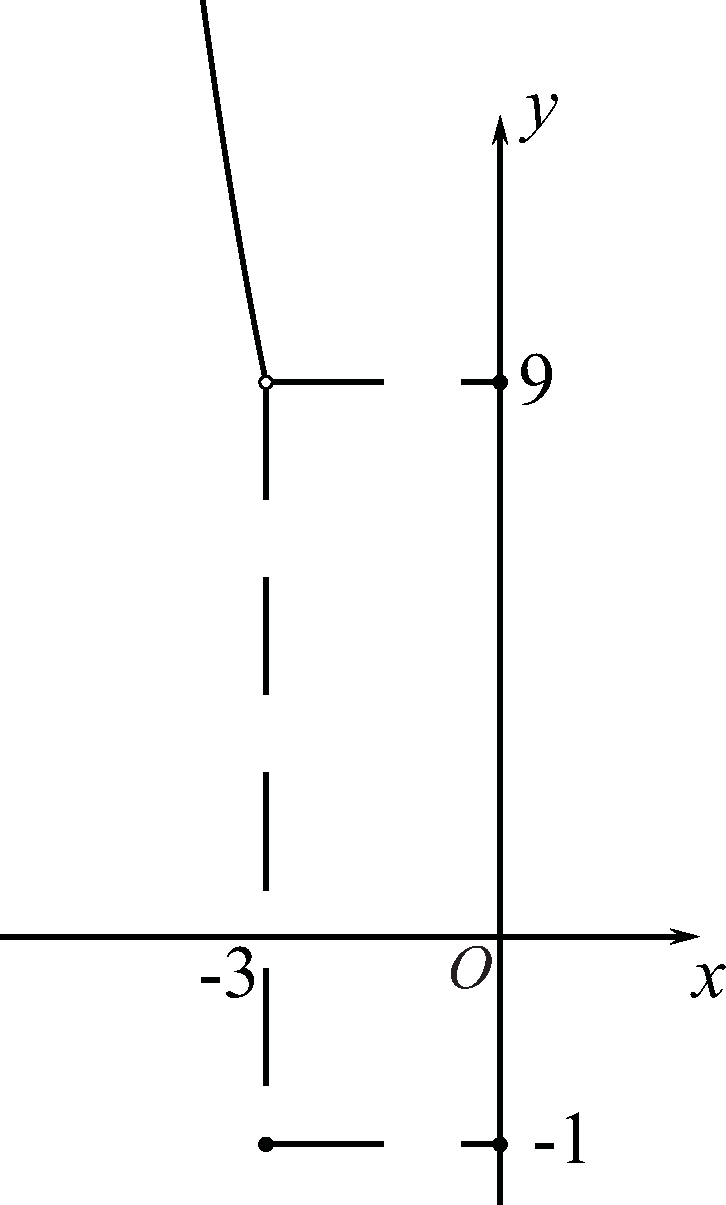
\includegraphics[width=\linewidth]{pic/C-1/可去间断点.pdf}
\end{tcolorbox}

\inference[判断间断点的类型]
\begin{center}
	\begin{tikzpicture}[node distance=1.2cm]
		%定义流程图具体形状
		\node (A) [minimum height=0cm,draw, node distance=1cm,inner sep=8pt] {\quad 判断$x$处是否有左右极限\quad \quad };
		\node (A2) [minimum height=0cm,draw, below of=A,node distance=1.2cm,inner sep=8pt,xshift =9cm] {无穷间断点/振荡间断点};
		\node (B) [minimum height=0cm,draw, below of=A,node distance=2.4cm,inner sep=8pt] {\quad   判断左右极限是否相等 \quad \quad  };
		\node (B2) [minimum height=0cm,draw, below of=B,node distance=1.2cm,inner sep=8pt,xshift =8.05cm] {跳跃间断点};
		\node (C) [minimum height=0cm,draw, below of=B,node distance=2.4cm,inner sep=8pt] {\quad   判断$x$ 处的函数值 \quad \quad  };
		\node (C2) [minimum height=0cm,draw, below of=C,node distance=1.2cm,inner sep=8pt,xshift =8.45cm] {函数在$x$处连续};
		\node (D) [minimum height=0cm,draw, below of=C,node distance=2.4cm,inner sep=8pt] {\quad   可去间断点 \quad \quad  };
		
		
		%连接具体形状
		\draw[arrows={-Stealth[scale=0.8]}](A) -- (B) node[midway,left=0.5cm,above=-0.3cm]{有} ;
		\draw[arrows={-Stealth[scale=0.8]}](A) --+(0,-1.2cm) node[midway,right=3.5cm,above=-0.3cm]{没有}|-(A2) ;
		\draw[arrows={-Stealth[scale=0.8]}](B) -- (C) node[midway,left=0.5cm,above=-0.3cm]{相等} ;
		\draw[arrows={-Stealth[scale=0.8]}](B) --+(0,-1.2cm) node[midway,right=3.5cm,above=-0.3cm]{不相等}|-(B2) ;
		\draw[arrows={-Stealth[scale=0.8]}](C) -- (D)node[midway,left=1.3cm,above=-0.3cm]{函数值$=$极限} ;
		\draw[arrows={-Stealth[scale=0.8]}](C) --+(0,-1.2cm) node[midway,right=3.5cm,above=-0.3cm]{函数值$\neq$极限/无定义}|-(C2) ;
	\end{tikzpicture}
\end{center}

\subsection{连续函数的运算}
\vspace*{-1em}

\theorem[连续函数的加减乘除]
设函数$f(x)$和$g(x)$在点$x_0$处连续,则它们的和(差)$f \pm g$、积$f \cot g$及商$\dfrac{f}{g}\,(g(x_0)\neq 0)$都在点$x_0$处连续.

\theorem[反函数的连续性]
如果函数$y=f(x)$在一个区间上连续且单调,那么它的反函数也在对应的区间连续且单调与原函数相同.


\theorem[复合函数的连续性\uppercase\expandafter{\romannumeral1}]
设函数$\lim\limits_{x \to x_0}g(x)=u_0$,,且函数$y=f(u)$在$u=u_0$处连续,则
\begin{equation}
	\lim\limits_{x \to x_0}f\big[g(x)\big]=\lim\limits_{u \to u_0}f(u)=f(u_0)
\end{equation}
\vspace*{-2em}

\warn
[
\hspace*{2em} $g(x)$可以不在点$x=x_0$处有连续,但是必须有极限.
]

\theorem[复合函数的连续性\uppercase\expandafter{\romannumeral2}]
设函数$u=g(x)$在$x=x_0$处连续,且$g(x_0)=u_0$,函数$y=f(x)$在$x=u_0$处连续,则复合函数$y=f\big[g(x)\big]$也在$x=x_0$处连续.\vspace*{1em}

\theorem[初等函数的连续性]
一切初等函数在其定义域内都是连续函数.\vspace*{1em}

\subsection{连续函数的性质}

\defination[最大值与最小值]
对于在区间$I$上有定义的函数$y=f(x)$,如果有$x_0 \in I$,使得任意一个$x$都有
\[
f(x)\le f(x_0)\quad\big(\,f(x) \geq f(x_0) \,\big)
\]
那么我们称$f(x_0)$是函数$y=f(x)$在区间$I$上的最大值(最小值).
\vspace*{1em}

\theorem[最大值最小值定理]
在闭区间上连续的函数在该区间上一定有界且一定能取到它的最大值和最小值.

\warn
[
\hspace*{2em} 如果函数在开区间内连续,或者在闭区间上有间断点,那么函数不一定有界且不一定能取到它的最大值或最小值.特别地,如果函数单调,且在开区间内连续,那么这个函数一定无界且无最大值和最小值.
]


\theorem[零点存在性定理]
设函数$f(x)$在闭区间$[a,b]$上连续,且$f(a)$与$f(b)$异号,即$f(a)\cdot f(b)<0$,则在开区间$(a,b)$内至少有一点$\xi$,使得
\[
f(\xi)=0
\]

\theorem[介值定理]
设函数$f(x)$在闭区间$[a,b]$上连续,且在这区间的取不同的函数值$f(a)=A,f(b)=B$,则对于$A$与$B$之间的任意一个数$C$,在开区间$(a,b)$内至少有一点$\xi$,使得
\[
f(\xi)=C(a<\xi<b)
\]

\tl 在闭区间$[a,b]$上连续的函数$f(x)$的值域为$[m,M]$,其中$m$与$M$依次为$f(x)$在$[a,b]$上的最小值与最大值.

\section{补充题型}
\subsection{求递归数列的极限}
\vspace*{-1em}

\example[求递归数列的极限]\vspace*{-1em}
\examples 已知$x_1>0,x_{n+1}=\dfrac{1}{2}\left(x_n+\dfrac{a}{x_n}\right),(a>0,n=1,2,\ldots),$证明$\lim\limits_{n \to \infty} x_n$存在,并求该极限.

\solve $\displaystyle x_{n+1}=\frac 12\left(x_n+\frac{a}{x_n}\right)\ge \frac 12 \cdot 2\sqrt{x_n\cdot \frac{a}{x_n}}=\sqrt{a}$,所以$n>2$时,$x_n \ge \sqrt{a},$又
\[
x_{n+1}-x_n=\frac{1}{2}\left(\frac{a}{x_n}-x_n\right)\le\frac{1}{2}\left(\frac{a}{\sqrt{a}}-\sqrt{a}\right)=0
\]
所以数列$\{x_n\}$是单调递减数列,所以$\max x_n=\max\{x_1,x_2\}$,即$0<x_n<\max{x_1,x_2}$,即$\{x_n\}$是有界数列.
综上,数列$\{x_n\}$是单调有界数列,由极限存在法则知$\lim\limits_{n \to \infty}x_n$一定存在.设$\lim\limits_{n \to \infty}x_n=\lim\limits_{n \to \infty}x_{n+1}=c>0.$则$n \to \infty$时,有
\[
x_{n+1}=\frac{1}{2}\left(x_n+\frac{a}{x_n}\right)\,(n \to \infty) \quad \Rightarrow \quad c=\frac 12\left( c+\frac ac \right) \quad \Rightarrow \quad c^2=a \quad \Rightarrow \quad c=\sqrt{a}. 
\]
故$\lim\limits_{n \to \infty}x_n=\sqrt{a}.$

\examples 已知$x_1=1,x_{n+1}=\sqrt{2+x_n},\,(n=1,2,\ldots),$证明$\lim\limits_{n \to \infty }x_n$存在,并求该极限.

\solve 下面用数学归纳法证明$x_n<2$.
\begin{enumerate}[(i)]
	\item 当$n=1$时,$x_n=x_1=1<2$成立.
	\item 设$n=k$时,$x_n=x_k<2$成立.
	\item 当$n=k+1$时,$x_n=x_{k+1}=\sqrt{2+x_k}<\sqrt{2+2}=2,$也成立.
\end{enumerate}
所以$0<x_n<2.$故数列$\{x_n\}$是有界数列.又
\[
x_{n+1}-x_n=\sqrt{2+x_n}-x_n=\frac{2}{\sqrt{2+x_n}+x_n}>0.
\]
所以数列$\{x_n\}$是单调递增数列,又数列$\{x_n\}$有界,故数列$\{x_n\}$是单调有界数列,由极限存在法则可知$\lim\limits_{n \to \infty}x_n$一定存在.设$\lim\limits_{n \to \infty}x_n=\lim\limits_{n \to \infty}x_{n+1}=c>0.$则$n \to \infty$时,有
\[
x_{n+1}=\sqrt{2+x_n} \quad \Rightarrow \quad c=\sqrt{2+c} \quad \Rightarrow \quad c^2-c-2=0 \quad \Rightarrow \quad (c-2)(c+1)=0 \quad \Rightarrow \quad c=2.
\]
故$\lim\limits_{n \to \infty}x_n=2.$

\inference[求递归数列的极限]
\vspace*{1em} \noindent  \hspace*{0.2em}  \tcbox[colframe =ForestGreen
, colback =ForestGreen!15!white,boxrule=0.5mm,size=small,on line]{\color{ForestGreen}{{\CJKfamily{heiti}题目模板}}}\hspace{1.5em}
已知$x_1=a,x_{n+1}=f(x_n),$判断$\lim\limits_{n \to \infty }x_n$是否存在,若存在则求该极限.\vspace*{1em}\vspace*{1em}

\noindent \highlights[第一步 \quad 找答案]

做这类题,首先要做的就是先把答案猜出来,具体方法如下:
假设$\lim\limits_{n \to \infty}x_n$存在,且$x_n>0$,得到式子$\lim\limits_{n \to \infty}x_{n+1}=c>0$,即$c=f(c)$,求出$c$的值.($x_n<0$类似)
\begin{enumerate}[(i)]
	\item 若无解,则$\lim\limits_{n \to \infty}x_n$不存在;
	\item 若有解,注意判断解的合理性,通常只有一个解$c_0>0\big(x_n>0\big)$或$c_0<0\big(x_n<0\big)$,则$\lim\limits_{n \to \infty}x_n=c_0$.
\end{enumerate}
\vspace*{1em}

\noindent \highlights[第二步 \quad 证有界]

由上面的极限可以知道,
\begin{enumerate}[]
	\item 若数列$\{x_n\}$单调递增,则证$x_n \le c_0$;
	\item 若数列$\{x_n\}$单调递减,则证$\max \{x_1,x_2\} \ge x_n \ge c_0$.
\end{enumerate}
\vspace*{-1em}
\warn
[
\hspace*{2em} 可以先不证明数列的单调性,但是要用赋值法先确定数列的单调性,就可以找到证明的方向,就可以容易用数学归纳法证明.
]
\vspace*{1em}

\noindent \highlights[第三步 \quad 证单调]

证单调直接用定义即可:\vspace*{-1em}
\begin{multicols}{2}
	\noindent1.$\,\,x_{n+1}-x_n=f(x_n)-x_n$.
	\begin{enumerate}[(i)]
		\item $x_{n+1}-x_n>0\Rightarrow\{x_n\}$是单调递增数列;
		\item $x_{n+1}-x_n<0\Rightarrow\{x_n\}$是单调递减数列.
	\end{enumerate}
	2.$\,\,\dfrac{x_{n+1}}{x_n}=\dfrac{f(x_n)}{x_n}$.
	\begin{enumerate}[(i)]
		\item $x_{n+1}/x_n>1\Rightarrow \{x_n\}$是单调递增数列;
		\item $x_{n+1}/x_n<1\Rightarrow \{x_n\}$是单调递减数列;
	\end{enumerate}
\end{multicols}
\vspace*{-1em}
\warn
[
\hspace*{2em} 在有变号的数列中第二种方法不适用.
]
\vspace*{1em}

\noindent \highlights[第四步 \quad 求极限]

由于$x_n$单调有界,由极限存在法则可知$\lim\limits_{x_n}$一定存在.$\lim\limits_{n \to \infty}x_n=\lim\limits_{n \to \infty}x_{n+1}=c>0,$即$c=f(c)$,求解这个方程后可以求出$c$的值,在步骤一中已经求出,可以直接写结果.
\warn
[
\hspace*{2em} $\lim\limits_{n \to \infty}x_n=\lim\limits_{n \to \infty}x_{n+1}=c$成立的前提条件是数列${x_n}$单调有界(或$\{x_n\}$收敛).
]

\subsection{极限存在求参数}
\vspace*{-1em}

\example[极限存在求参数]\vspace*{-1em}

\examples 求实数$a,b$使得
\[
\lim\limits_{x \to 1}\frac{\sqrt{ax^2-2ax+b}-2}{x^2-2x+1}
\]
存在,并求出该极限.

\solve 由于$\lim\limits_{x \to 1}(x^2-2x+1)=0$.即分母为无穷小量.要使极限存在,则分子也为无穷小量,即
\[
\lim\limits_{x \to 1}\big[\sqrt{ax^2-2ax+b}-2\big]=0 \quad \Rightarrow \quad \sqrt{a-2a+b}-2=0 \quad \Rightarrow \quad \sqrt{b-a}=2 \quad \Rightarrow b-a=4.
\]
代入原极限式,并令$t=x-1,$,则$x=t+1,x\to1,t \to 0,$可得
\[
\begin{split}
	\lim\limits_{x \to 1}\frac{\sqrt{ax^2-2ax+b}-2}{x^2-2x+1}&=\lim\limits_{t \to 0}\frac{\sqrt{at^2+b-a}-2}{t^2}=\lim\limits_{t \to 0}\frac{\sqrt{at^2+4}-2}{t^2}\\
	&=\lim\limits_{t \to 0}\frac{at^2}{t^2\big(\sqrt{at^2+4}+2\big)}=\lim\limits_{t \to 0}\frac{a}{\sqrt{at^2+4}+2}=\frac{a}{4}.
\end{split}
\]
所以,当$b-a=4$时,均有
\[
\lim\limits_{x \to 1}\frac{\sqrt{ax^2-2ax+b}-2}{x^2-2x+1}=\frac a4.
\]

\examples 求实数$a,b$使得
\[
\lim\limits_{x \to 0}\frac{1+a\cos2x+b\cos4x}{x^4}
\]
存在,并求该极限.

\solve 
\[
\begin{split}
	\lim\limits_{x \to 0}\frac{1+a\cos2x+b\cos4x}{x^4}&=\lim\limits_{x \to 0}\frac{1+a\cos2x+b\cos4x}{x^4}\\
	&=\lim\limits_{x \to 0}\frac{1+a\cos 2x+b(2 \cos^22x-1)}{\big(\sin^2x\big)^2}\\
	&=\lim\limits_{x \to 0}\frac{1+a\cos 2x+2b \cos^22x-b}{\left(\frac{\cos 2x-1}{2}\right)^2}\\
	&=4\lim\limits_{x \to 0}\frac{2b\left(\cos^2 2x+\frac{a}{2b}\cos 2x +\left( \frac{a}{2b}\right)^2 -\frac{a^2}{16b^2}  \right)+1-b }{\left(\cos 2x-1\right)^2}\\
	&=4\lim\limits_{x \to 0}\frac{2b\left(\cos^2 2x+\frac{a}{2b}\cos 2x +\left( \frac{a}{2b}\right)^2 \right)+1-\frac{a^2}{8b} -b }{\left(\cos 2x-1\right)^2}\\
	&=4\lim\limits_{x \to 0}\frac{2b\left(\cos 2x +\frac{a}{4b}\right)^2+1-\frac{a^2}{8b} -b }{\left(\cos 2x-1\right)^2}\\
\end{split}
\]
要使极限存在,则要消去分母$\left(\cos 2x-1\right)^2$,比对系数得:
\[
\begin{cases}
	\dfrac{a}{4b}=-1\\[0.5em]
	1-\dfrac{a^2}{8b}-b=0
\end{cases}
\quad 
\Rightarrow
\quad 
\begin{cases}
	a=-\dfrac{4}{3}\\[0.5em]
	b=\dfrac{1}{3}
\end{cases}
\]
综上,当
$
\begin{cases}
	a=-\dfrac{4}{3}\\[0.5em]
	b=\dfrac{1}{3}
\end{cases}
$
时,极限
$
\lim\limits_{x \to 0}\dfrac{1+a\cos2x+b\cos4x}{x^4}
$
存在,且为$\dfrac{8}{3}.$

\subsection{分数型极限}
\vspace*{-1em}

\example[分数型极限]
关于这个题型先给出一个定理.

\theorem[分数型极限]
\begin{equation}
	\lim\limits_{x \to \infty}\frac{a_nx^n+a_{n-1}x^{n-1}+\cdots+a_2x^2+a_1x+a_0}{b_mx^m+b_{m-1}x^{m-1}+\cdots+b_2x^2+b_1x+b_0}=
	\begin{cases}
		0&,n<m\\
		\dfrac{a_n}{b_m}&,n=m\\
		\infty&,n>m
	\end{cases}
\end{equation}
\begin{equation}
	\lim\limits_{x \to 0}\frac{a_nx^n+a_{n-1}x^{n-1}+\cdots+a_2x^2+a_1x+a_0}{b_mx^m+b_{m-1}x^{m-1}+\cdots+b_2x^2+b_1x+b_0}=
	\begin{cases}
		\infty&,n<m\\
		\dfrac{a_n}{b_m}&,n=m\\
		0&,n>m
	\end{cases}
\end{equation}
\warn
[
\hspace*{2em} 这个定理只适合变量趋于0或$\infty$的情况.
]
通常这种类型还有几种变形,下面给出一个例子.

\examples 求极限$\lim\limits_{x \to +\infty}\dfrac{(x+1)(x^2+1)\cdot\,\cdots\,\cdot(x^n+1)}{\big[(nx)^n+1\big]^{\frac{n+1}{2}}}$.

\solve 由上面的定理可知,我们只需要考虑分子和分母的最高次项即可.\\[0.5em]
因为$(x+1)(x^2+1)\cdots(x^n+1)$的最高次项为$\displaystyle x^{\frac{n(n+1)}{2}}$,$\big[(nx)^n+1\big]^{\frac{n+1}{2}}$的最高次项为$\displaystyle (nx)^{\frac{n(n+1)}{2}}$.所以
\[
\lim\limits_{x \to +\infty}\dfrac{(x+1)(x^2+1)\cdot\,\cdots\,\cdot(x^n+1)}{\big[(nx)^n+1\big]^{\frac{n+1}{2}}}=\lim\limits_{x \to +\infty}\dfrac{x^{\frac{n(n+1)}{2}}}{(nx)^{\frac{n(n+1)}{2}}}=\frac{1}{n^{\frac{n(n+1)}{2}}}.
\]

\vspace*{-2em}
\summarize
[
\hspace*{2em} 其实看起来解题过程比较复杂,但是其实本质比较简单,弄清楚这种题型的做题方法如下:\\
1. 观察式子,判断题型是否为分数型;\\
2. 确定为分数型题型后,判断分数的分母和分子最高的次数的大小;\\
3. 运用定理运算极限即可.\\
\hspace*{2em} 特别注意的是,有些时候不是很好判断是否为分数型,像上面的例题.这个时候可以观察分子分母是否是高次多项式.如果分子和分母都是高次多项式,那么就可以尝试用分数型的解题方法来尝试解题.\\
\hspace*{2em} 可能还有的题需要换元以后才能得到这个分数型极限.
]

\subsection{已知一个极限式求另一极限式}
\examples 若$\displaystyle \lim\limits_{x \to 0}\left(\frac{f(x)-1}{x}-\frac{\sin x}{x^2}\right)=2$,求$\lim\limits_{x \to 0}f(x).$

\solve 记$\alpha = \dfrac{f(x)-1}{x}-\frac{\sin x}{x^2},$由题可知$\lim\limits_{x \to \alpha =0},$即
\[
f(x)=1+\alpha x+\frac{\sin x}{x}+2x \quad \Rightarrow \quad \lim\limits_{x \to 0}f(x)=\lim\limits_{x \to 0}\left( 1+ \alpha x +\frac{\sin x}{x} +2x\right) 
\]
由极限四则运算,得
\[
\lim\limits_{x \to 0}f(x)=\lim\limits_{x \to 0}\left( 1+ \alpha x +\frac{\sin x}{x} +2x\right) =1+0+1+0=2.
\]
\vspace*{-1em}
\summarize
[
\hspace*{2em} 这是一类知道含$f(x)$的多项式的极限,求$\lim f(x)$的一类题,很巧妙地运用了换元法.
]

\subsection{求和式的极限}
\vspace*{-1em}

\example[求和式的极限]
求和式的极限在高等数学教材中目前有两种可行的方法:定积分法和夹逼定理法.\vspace*{1em}

\noindent \highlights[1.定积分法]

如果函数$y=f(x)$在区间$[a,a+\lambda]$上可积,那么由定积分的定义可知定积分的值与区间的分割方式无关,那么我们将区间$[a,a+\lambda]$进行$n$等分;定积分的值也与$\xi_i$的取法无关,那么在分割后的每个小区间$[x_i,x_{i+1}]$中$\xi_i$取$x_i$,那么这样以后,我们就有:
\begin{equation}
	S=\int_{a}^{a+\lambda}f(x)\,\d x=\lim\limits_{n \to \infty}\sum_{i=1}^{n}f(x_i)\cdot \Delta x_i
	\label{定积分定义}
\end{equation}
由于区间$[a,a+\lambda]$$n$等分,那么
\begin{equation}
	\Delta x_i = \frac{a+\lambda -a}{n}=\frac{\lambda}{n}
\end{equation}
\begin{equation}
	x_i=a_i\cdot \Delta x_i=a+\frac{\lambda i}{n}
\end{equation}
代入\eqref{定积分定义}得,
\begin{equation}
	S=\int_{a}^{a+\lambda}f(x)\,\d x=\lim\limits_{n \to \infty}\sum_{i=1}^{n}f(x_i)\cdot \Delta x_i=\lim\limits_{n \to \infty}\sum_{i=1}^{n}f\left(a+\frac{\lambda i}{n}\right)\cdot \frac{\lambda}{n}=\lim\limits_{n \to \infty} \frac{\lambda}{n}\cdot \sum_{i=1}^{n}f\left(a+\frac{\lambda i}{n}\right)
\end{equation}
即
\begin{equation}
	\lim\limits_{n \to \infty} \frac{\lambda}{n}\cdot \sum_{i=1}^{n}f\left(a+\frac{\lambda i}{n}\right)=\int_{a}^{a+\lambda}f(x)\,\d x
\end{equation}
特别地,当$a=0$时,有
\begin{equation}
	\lim\limits_{n \to \infty} \frac{\lambda}{n}\cdot \sum_{i=1}^{n}f\left(\frac{\lambda i}{n}\right)=\int_{0}^{\lambda}f(x)\,\d x
\end{equation}
进一步,如果$\lambda =1$,那么
\begin{equation}
	\lim\limits_{n \to \infty} \frac{1}{n}\cdot \sum_{i=1}^{n}f\left(\frac{ i}{n}\right)=\int_{0}^{1}f(x)\,\d x
\end{equation}

这样定积分就为我们求和式的极限在$n \to \infty$时的值给出了一个较为简单的算法.为此,我们需要构造如下的形式:
\begin{equation}
	\lim\limits_{n \to \infty} \frac{1}{n}\cdot \sum_{i=1}^{n}f\left(\frac{i}{n}\right)
\end{equation}
即找到关于$\dfrac{i}{n}$的函数$f\left(\dfrac{i}{n}\right)$.\\[0.5em]
下面给出几个典型的例题.

\examples 求极限$\displaystyle \lim\limits_{n \to \infty}\frac 1n \sum_{k=1}^{n}\frac{1}{1+\left( \frac{k}{n}\right)^2 }$.

\solve $\displaystyle \lim\limits_{n \to \infty}\frac 1n \sum_{k=1}^{n}\frac{1}{1+\left( \frac{k}{n}\right)^2 }=\int_{0}^{1}\frac{1}{1+x^2}\,\d x=[\arctan x]_0^1=\frac{\pi}{4}-0=\frac{\pi}{4}=\frac{\pi}{4}.$

\summarize
[
\hspace*{2em} 本题的被积函数为$f(x)=\dfrac{1}{1+x^2},$可以代入验证$\displaystyle f\left(\dfrac{k}{n} \right)=\dfrac{1}{\textstyle 1+\left(\frac{k}{n} \right)} $.
]
\clearpage
\vspace*{-3em}
\examples 求极限$\displaystyle \lim\limits_{n \to \infty}\sum_{k=1}^{n}\frac{k^4}{n^5 }$.

\solve $\displaystyle \lim\limits_{n \to \infty}\sum_{k=1}^{n}\frac{k^4}{n^5 }=\lim\limits_{n \to \infty} \frac 1n \sum_{k=1}^{n}\frac{k^4}{n^4}=\lim\limits_{n \to \infty} \frac 1n \sum_{k=1}^{n}\left( \frac{k}{n}\right)^4=\int_{0}^{1} x^4 \, \d x = \left[\frac 15 x^5 \right]_0^1=\frac 15-0=\frac 15.$
\vspace{1em}

\examples 求极限$\displaystyle \lim\limits_{n \to \infty}\sum_{k=1}^{n}\frac{2}{n}\cdot \left[3\left( 1+\dfrac{2k}{n}\right)  -6\right] $.

\solve 
$
\displaystyle
\lim\limits_{n \to \infty}\sum_{k=1}^{n}\frac{2}{n}\cdot \left[3\left( 1+\dfrac{2k}{n}\right)  -6\right]
=\lim\limits_{n \to \infty}\frac{2}{n} \cdot \sum_{k=1}^{n}\left[3\left( 1+\dfrac{2k}{n}\right)  -6\right]
=\int_{0}^{2}[3(1+x)^5-6]\,\d x
$
\begin{align*}
	&=3\int_{0}^{2}(1+x)^5\,\d(1+x)-6\int_{0}^{2}\,\d x=3\int_{1}^{3}t^5\,\d t-6\int_{0}^{2}\,\d x=3\left[\frac 16 t^6\right]_1^3-6[x]_0^2=\frac{1}{2}(3^6-1)-6(2-0)\\
	&=\frac 12(729-1)-12=364-12=352.
	\vspace*{-2em}
\end{align*}

\summarize
[
\hspace*{2em} 此题被分割的区间上限不再是 1, 而是 2, 在做题需要注意分割区间($\lambda$的值),不要直接认为是 1.
]

\examples 求极限$\displaystyle \lim\limits_{n \to \infty}\left[ \frac 1n +\frac {1}{n+1}+\cdots+\frac{1}{3n}\right] $.

\solve 
$
\displaystyle
\lim\limits_{n \to \infty}\left[ \frac 1n +\frac {1}{n+1}+\cdots+\frac{1}{3n}\right] 
=\lim\limits_{n \to \infty}\sum_{k=0}^{2n}\frac{1}{n+k}
=\lim\limits_{n \to \infty}\frac{1}{2n}\cdot \sum_{k=0}^{2n}\frac{2n}{n+k}
=\lim\limits_{n \to \infty}\frac{1}{2n}\cdot \sum_{k=0}^{2n}\frac{1}{\frac{1}{2}+\frac{k}{2n}}
$
\[
=\int_{0}^{1}\frac{2}{1+2x}\,\d x=\big[\ln(1+2x)\,\big]_0^1=\ln 3.
\vspace*{-0.5em}
\]

\summarize
[
\hspace*{2em} 本题没有给出和式表达式,需要我们自己写成和式的形式,以方便构造积分的形式.\\
\hspace*{2em} 本题中和式的上限不是$n$而是$2n$,那么这个时候整个积分区间就不是被等分成$n$份,而是$2n$份,因此,我们要构造关于变量$\dfrac{i}{2n}$的函数,即
\begin{equation}
	\lim\limits_{n \to \infty}\frac{1}{2n}\cdot\sum_{i=1}^{2n}f\left(\frac{i}{2n}\right)
\end{equation}
\hspace*{2em} 积分的上下限由变量$\dfrac{i}{n}$(本题$\dfrac{i}{2n}$)的范围所确定,如本题$i =1,2,\ldots,2n,\lim\limits_{n \to \infty}\dfrac{i}{2n}=0,1.$.因此积分的上下限是0,1.
]
\vspace{1em}

\noindent \highlights[2. 夹逼定理法]

\vspace*{1em} \noindent  \hspace*{0.2em}  \tcbox[colframe =ForestGreen
, colback =ForestGreen!15!white,boxrule=0.5mm,size=small,on line]{\color{ForestGreen}{{\CJKfamily{heiti}总思路}}}\hspace{1.5em}
设求$\lim\limits_{n \to \infty}f(n),$其中$\lim\limits_{n \to \infty}f(n)$是无穷多个式子之和.\\[0.2em]
\qquad (1) \quad 将$f(n)$的所有项都缩小为所有项中的最小值求和化简得到式$f_{\min}(n)$,\\[0.2em]
\qquad (2) \quad 将$f(n)$的所有项都放大为所有项中的最大值求和化简得到式$f_{\max}(n)$,\\[0.2em]
\qquad (3) \quad 证明$\lim\limits_{n \to \infty}f_{\min}(n)=\lim\limits_{n \to \infty}f_{\max}(n)=c.$\\[0.2em]
从而$\lim\limits_{n \to \infty}f(n)=\lim\limits_{n \to \infty}f_{\min}(n)=\lim\limits_{n \to \infty}f_{\max}(n)=c.$

\clearpage
\examples 求极限$\displaystyle \lim\limits_{n \to \infty}\left(\frac{1}{n^2+n+1}+\frac{2}{n^2+n+2}+\cdots+\frac{n}{n^2+n+n}\right)$

\solve 因为$1 \le i \le n$时,$\displaystyle \frac{i}{n^2+n+n}\le\frac{i}{n^2+n+i}\le \frac{i}{n^2+n+1}$,则
\[
\frac{1+2+\cdots+n}{n^2+n+n}\le \frac{1}{n^2+n+1}+\frac{2}{n^2+n+2}+\cdots+\frac{n}{n^2+n+n} \le \frac{1+2+\cdots+n}{n^2+n+1}
\]
又
\[
\lim\limits_{n \to \infty}\frac{1+2+\cdots +n}{n^2+n+n}=\frac 12 \cdot \lim\limits_{n \to \infty}\frac{n(1+n)}{n(n+2)}=\frac 12 \cdot \lim\limits_{n \to \infty}\frac{n+1}{n+2}=\frac{1}{2}.
\]

\[
\lim\limits_{n \to \infty}\frac{1+2+\cdots +n}{n^2+n+1}=\frac 12 \cdot \lim\limits_{n \to \infty}\frac{n(1+n)}{n^2+n+1}=\frac 12 \cdot \lim\limits_{n \to \infty}\frac{n^2+n}{n^2+n+1}=\frac{1}{2}.
\]
\\
故
$
\displaystyle \lim\limits_{n \to \infty}\frac{1+2+\cdots +n}{n^2+n+n}=\lim\limits_{n \to \infty}\frac{1+2+\cdots +n}{n^2+n+1}=\frac 12.
$
由夹逼定理可知
\[
\lim\limits_{n \to \infty}\left(\frac{1}{n^2+n+1}+\frac{2}{n^2+n+2}+\cdots+\frac{n}{n^2+n+n}\right)=\frac 12.
\]

\vspace*{-1.5em}
\summarize
[
\hspace*{2em} 对于含有分式的和式,一般先观察式子,如果分母的次数比分子高2次(或者更高),那么夹逼法则一定能做.\\
如果分母的次数仅比分子高1次,那么我们可以尝试用方法一定积分来做.
]

\examples 求极限$\lim\limits_{n \to \infty}\sqrt[n]{a_z^n+a_2^n+\cdots+a_m^n}\,\big(n,m \in \mathbb{N}^*,i=1,2,\ldots,m \big)$.

\solve 不妨设$M=\max{a_1,a_2,\ldots,a_m}$,则
\[
M=\sqrt[n]{M}\le \sqrt[n]{a_z^n+a_2^n+\cdots+a_m^n} \le \sqrt[n]{mM^n}=\sqrt[n]{m}\cdot M
\]
而$\lim\limits_{n \to \infty}\sqrt[n]{m}=1,\lim\limits_{n \to \infty }\sqrt[n]{m}\cdot M=M$,由夹逼定理可知
\[
\lim\limits_{n \to \infty}\sqrt[n]{a_z^n+a_2^n+\cdots+a_m^n}=M.
\]

\summarize
[
\hspace*{2em} 对于未知大小的元素之和,可以先规定最大值(最小值),方便计算.
]
	
	% 第二章:自动控制系统的数学模型
	\chapter{航天器姿态动力学}
\thispagestyle{empty}
\section{动力学建模方法简述}
研究{\color{dy} 角速度$\bm{\omega}_{ba}$的变化与作用力矩之间的关系}的学科称为\dy[姿态动力学]{ZTDLX}。一般有以下几个建模方法。
\vspace*{1em}

\sssection[矢量力学法(牛顿—欧拉法)\index{SLLXF@矢量力学法} \index{NDOLF@牛顿欧拉法}]

采用动力学基本定理(即牛顿运动方程的直接推论),给出系统动力学量与作用于该系统的力之间的关系。即\dy[动量定理]{DLDL}、\dy[动量矩定理]{DLJDL}。
\vspace*{1em}


\sssection[分析力学法\index{FXLXF@分析力学法}]

从系统能量观点出发,运用现代力学的\dy[拉格朗日法]{LGLRF}或\dy[哈密顿法]{HMDF}导出系统的动力学方程。能自动消除物体间的约束力和约束反力,缺点是对于复杂结构,推导工作量大。
\vspace*{1em}


\sssection[矢量力学与分析力学的各种变形方法]

凯恩(Kane)方法、R/W方法、旋量方法、高斯最小约束原理方法等。




\section{刚体的姿态动力学建模原理}
\subsection{单质点的动量矩定理}

如图 \ref{单质点角动量} 所示,坐标系$O'XYZ$是一个惯性坐标系,$O$是其中的一个动参考点,以$O$为原点建立一个动坐标系$oxyz$。

\begin{figure}[!htb]
	\centering
	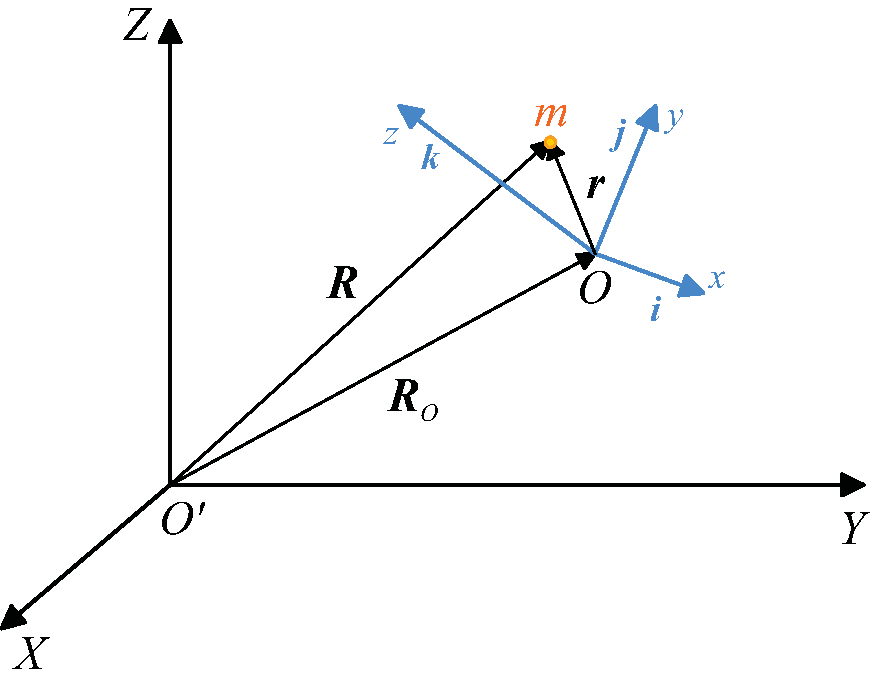
\includegraphics[width=0.4\linewidth]{pic/单质点角动量}
	\vspace*{-1em}
	\caption{质点$m$关于任意参考点$O$的角动量}
	\label{单质点角动量}
\end{figure}

在动坐标系中存在一个质量为$m$的质点,其\dy[线动量]{XDL}为
\begin{equation}
	\bm{p} = m \dot{\bm{R}}
	\nomenclature{$\bm{p}$}{质点的线动量 \nomrefpage}
\end{equation}
其中,$\bm{R}$为质点相对于惯性坐标系的位置向量(绝对位置向量)。

质点$m$的动量$\bm{p}$关于参考点$O$的\dy[角动量]{JDL}(或\dy[动量矩]{DLJ})定义为
\begin{equation}
	\bm{H}^O = \bm{r} \times m \dot{\bm{R}}
	\nomenclature{$\bm{H}^O$}{质点关于参考点$O$的角动量 \nomrefpage}
\end{equation}
其中,$\bm{r}$为质点$m$相对于参考点$O$的位置向量(相对位置向量)。由于$\bm{R} = \bm{R}_O + \bm{r}$,则有$\dot{\bm{R}} = \dot{\bm{R}}_O + \dot{r}$,那么
\begin{equation}
	\ubm{H}^O = \bm{r} \times m \dot{\bm{r}} + \bm{r} \times m \dot{\bm{R}}_O
	\label{H1}
\end{equation}
其中,公式 \eqref{H1} 右侧第一项$\bm{r} \times m \dot{\bm{r}}$称为动坐标系$Oxyz$中的\dy[视角动量]{SJDL},用$\bm{H}^{\underline{O}}$表示;而另一项是因为点$O$运动引起的修正项。
\nomenclature{$\bm{H}^{\underline{O}}$}{质点的视角动量 \nomrefpage}


























	
	\chapter{动量与角动量}
\thispagestyle{empty}
\section{对质点的动量定理}
质点所受的和外力的冲量等于该质点动量的增量,即
\margin{动量定理说明力对质点作用的时间积累效果表现为质点动量的改变.它是牛顿第二定律的直接变形,故也只适用于惯性系.}
\begin{equation}
\bm{F} \d t=\d \bm{p}=\d (m\bm{v})
\end{equation}
或
\begin{equation}
\int_{0}^{t} \bm{F}\d t= \bm{p}-\bm{p}_0=m\bm{v}-\bm{v}_0
\end{equation}

\section{对质点系的总动量}
质点系的总动量
\begin{equation}
\bm{p}=\sum\bm{p}_i=\sum m_i\bm{p}_i
\end{equation}
作用于质点系的外力的矢量和为合外力
\begin{equation}
\bm{F}=\sum\bm{F}_i
\end{equation}
\par \dy[质点系的动量定理]{ZDXDDLDL}
\begin{equation}
\bm{F}\d t = \d \bm{p}\quad \quad \left( \bm{F}=\frac{\d \bm{p}}{\d t}\right) 
\end{equation}
\par \dy[动量守恒定律]{DLSHDL}\jg
\margin{在外力远小于内力的情况下,外力对质点系的总动量变化影响很小,这时近似满足动量守恒的条件.例如,两个物体的碰撞和爆炸过程.}
\par 当系统所受的合外力为0时,系统的总动量不随时间改变.\jg
\par \dy[孤立系统]{GLXT} 一个不受外界影响的系统.一个孤立系统在运动过程中,其动量一定保持不变.

\section{火箭飞行原理}
假设火箭在自由空间飞行,即不受引力或空气阻力等任何外力的影响.质量为$M$,此时速度为$v$的火箭经过$\d t$时间喷出$\d m$质量的气体,喷出速率相对与火箭为定值$u$.则由动量守恒定律,
\margin{\\[1.5em]\kg 注意到$\d m=-\d M$}
\begin{equation*}
\d m\cdot (v-u)+(M-\d m)(v+\d v)=-\d M\cdot (v-u)+(M+\d M)(v+\d v)=Mv
\end{equation*}
忽略二阶无穷小量$\d M \cdot \d v$可得
\begin{equation*}
u\d M+M\d v=0
\end{equation*}
即
\margin{$M_i$为点火时的质量,\\\kg $v_i$为初速度.\\\kg$v_f$为末速度.\\\kg$M_f$为燃料耗尽时质量.}
\begin{equation*}
v_f-v_i=u\ln\frac{M_i}{M_f}
\end{equation*}
\par 如果只以火箭本身为研究的系统,以$F$表示在时间间隔$t$到$t+\Delta t$内喷出气体对火箭体(质量为$(M-\d m)$)的推力,由动量定理,有
\begin{equation*}
F\d t=(M-\d m)[(v+\d v)-v]=M\d v
\end{equation*}
由$M\d v=-u\d M=u \d m$代入,得
\begin{equation*}
F=u\frac{\d m}{\d t}
\end{equation*}
说明火箭发动机的推力与燃料的燃烧速率$\d m/\d t $以及喷出气体的相对速率$u$成正比.

\section{质心}
\dy[质心]{ZX} 质心是相对于质点系各质点位置分布的一个特殊点
\margin{\\[1em] \kg{\scriptsize{$\disp m=\sum m_i$}},\\\kg $\bm{r_i}$ 为$m_i$质点的位矢.}
\begin{equation}
\bm{r}_C=\frac{\sum m_i \bm{r}_i}{m}\quad \mbox{或}\quad \bm{r}_C=\frac{\int \bm{r} \d m}{m}
\end{equation}
其坐标分量为
\margin{\\[3em] \kg 均质几何体的质心就在其几何中心.}
\begin{equation}
\begin{cases}
\displaystyle 
x_C=\frac{\sum m_ix_i}{m}\\
\\
\displaystyle 
y_C=\frac{\sum m_iy_i}{m}\\
\\
\displaystyle 
z_C=\frac{\sum m_iz_i}{m}
\end{cases}
\quad \mbox{或}\quad 
\begin{cases}
\displaystyle 
x_C=\frac{\int x \d m}{m}\\
\\
\displaystyle 
y_C=\frac{\int y \d m}{m}\\
\\
\displaystyle 
z_C=\frac{\int z \d m}{m}
\end{cases}
\end{equation}

\par \dy[质心的速度]{ZXDSD}
\begin{equation}
\bm{v}_C=\frac{\d \bm{r}_C}{\d t}=\frac{\sum m_i\bm{v}_i}{m}
\end{equation}

\par \dy[质心的加速度]{ZXDJSD}
\begin{equation}
\bm{a}_C=\frac{\d \bm{v}_C}{\d t}=\frac{\sum m_i\bm{a}_i}{m}
\end{equation}

\par \dy[质心运动定理]{ZXYDDL}\jg
\par 质点系所受合外力等于质心系的总质量和其质心的加速度的乘积
\begin{equation}
\bm{F}=\frac{\d \bm{p}}{\d t}=m\bm{a}_C
\end{equation}

\newpage
\section{对质点的角动量定理}
\dy[质点的角动量]{ZDDJDL}
\margin{\\[1em] \kg 角动量的大小表示质点对一固定点的转动状态.\\\kg$\bm{r}$为质点相对于定点的位矢}
\begin{equation}
\begin{split}
\bm{L}&=\bm{r}\times \bm{p}=\bm{r}\times(m\bm{v})\\
L&=mrv\sin(\bm{r},\bm{v})
\end{split}
\end{equation}
\par \dy[力矩]{LJ}
\margin{\\[1em] \kg 力矩表示力对质点的转动作用.\\\kg$\bm{r}$为质点相对于定点的位矢}
\begin{equation}
\begin{split}
\bm{M}&=\bm{r}\times \bm{F}\\
M&=rF\sin(\bm{r},\bm{F})
\end{split}
\end{equation}
\par \dy[质点的角动量定理]{ZDDJDLDL}
\margin{特别地,如果$\bm{M}=0$,那么$\bm{L}$为常矢量,则质点对该定点角动量守恒.}
\begin{equation}
\bm{M}=\frac{\d \bm{L}}{\d t}
\end{equation}

\section{对质点系的角动量定理}
\dy[质点系的角动量]{ZDXDJDL}
\begin{equation}
\bm{L}=\sum \bm{L}_i=\sum \bm{r}_i\times \bm{p}_i
\end{equation}

\par \dy[质点系的力矩]{ZDXDLJ}
\begin{equation}
\bm{M}=\sum \bm{M}_i =\sum \bm{r}_i\times \bm{F}_i
\end{equation}
\par \dy[质点系的角动量定理]{ZDXDJDLDL}
\begin{equation}
\bm{M}=\frac{\d \bm{L}}{\d t}
\end{equation}
\par 特别地,当$\bm{M}=0$时,那么$\bm{L}$为常矢量,则质点系角动量守恒.也说明内力矩不能改变系统的总角动量.





	
	\chapter{根轨迹法}
\thispagestyle{empty}
\section{根轨迹与根轨迹方程}
\subsection{根轨迹}

\tdefination[根轨迹]
系统开环函数中某个参数(如开环增益$K$)从零到无穷时,闭环特征根$s$在复平面上的轨迹称为\dy[根轨迹]{GGJ}。
\begin{enumerate}[\hspace*{2em}(1)]
	\item 系统的动态特性主要取决于闭环极点在复平面上的位置。
	\item 在设计上,很多情形下只需调节开环增益的大小就可将闭环极点置于理想位置。
	\item 根轨迹本质上是通过开环传递函数某个参数(通 常是开环增益)的变化来研究闭环根轨迹。
\end{enumerate}
\vspace*{1em}

\subsection{闭环零点极点和开环零点极点的关系}
考虑典型闭环系统
\begin{figure}[!htb]
	\centering
	\begin{tikzpicture}[circuit ee IEC]
		\node(A) [draw, inner sep =6pt]{$G(s)$};
		\node(B) [draw, inner sep =6pt, below of = A, node distance = 1cm]{$H(s)$};
		\node[bulb] (O) [draw, inner sep =5pt, left of = A, node distance = 2cm, label = -95:$-$]{};
		
		\draw[arrows={-Stealth}](-3cm, 0) -- (O)node[near start, above = 0mm]{$R(s)$} -- (A)node[midway, above = 0mm]{$E(s)$} -- (2cm, 0cm)node[midway, above = 0mm,xshift = 5mm]{$C(s)$};
		\draw[arrows={-Stealth}](1.5cm, 0cm) -- +(0cm, -1cm) -- (B) -- (-2cm,-1cm) -- (O)node[midway, xshift =5mm,yshift =1mm]{$B(s)$};
	\end{tikzpicture}
	\caption{典型闭环系统}
\end{figure}

则闭环传递函数为
\begin{align}
	\varPhi (s) = \dfrac{G(s)}{1 + G(s)H(s)}
\end{align}
其中,
\begin{myitemize}
	\item $G(s)$\quad 前向通道传递函数\vspace*{-0.5em}
	\item $H(s)$ \quad 反馈通道传递函数\vspace*{-0.5em}
	\item $G(s)H(s)$\quad 开环传递函数\vspace*{0.3em}
\end{myitemize}
记
\begin{align*}
	G(s) = K^*_G\dfrac{\displaystyle \prod_{i = 1}^{f}(s - z_i)}{\displaystyle \prod_{i = 1}^q (s - p_i)},\quad \quad 
	H(s) = K^*_H\dfrac{\displaystyle \prod_{j = 1}^{l}(s - z_j)}{\displaystyle \prod_{j = 1}^h (s - p_j)}
\end{align*}
则
\begin{align}
	G(s)H(s) = K^*\dfrac{\displaystyle \prod_{i = 1}^{f}(s - z_i)\prod_{j = 1}^l (s - p_j)}{\displaystyle \prod_{i = 1}^q (s - p_i)\prod_{j = 1}^h (s - p_j)}, \quad \quad K^* = K_G^* K_H^*\\
	\varPhi(s) = \dfrac{\displaystyle K_G^*\prod_{i = 1}^{f}(s - z_i)\prod_{j = 1}{h}(s - p_j) }{\displaystyle \prod_{i = 1}^{q}(s - p_i) \prod_{j = 1}^{h} (s- p_j) + \textcolor{red}{K^*} \prod_{i = 1}^f(s - z_i) \prod_{j = 1}^l(s - z_j) } 
\end{align}
可以看出
\begin{itemize}
	\item 闭环系统零点由前向通道的零点和反馈通道的极点组成\vspace*{-0.5em}
	\item 闭环系统的极点与开环系统的极点零点以及开环根轨迹增益$K^*$有关
\end{itemize}
进一步化简$G(s)H(s)$,得
\begin{align}
	G(s)H(s) = K^*\dfrac{\displaystyle \prod_{j = 1}^{m}(s - z_j)}{\displaystyle \prod_{i = 1}^n (s - p_i)},\quad\quad n \ge m
	\label{GH}
\end{align}
其中,
\begin{myitemize}
	\item $K^*$ \quad 开环根轨迹增益\vspace*{-0.75em}
	\item $z_i\,\,$\quad 开环传递函数的零点\vspace*{-0.75em}
	\item $p_i$ \quad 开环传递函数的极点\vspace*{0.3em}
\end{myitemize}
\noindent 由此可知特征方程
\begin{align}
	D(s) =1 + G(s)H(s) = \prod_{i = 1}^n (s - p_i) + K^* \prod_{j = 1}^{m}(s - z_j) = 0
\end{align}

\noindent \textbf{根轨迹法的任务}

在已知开环零、极点分布的情况下,通过图解法求出闭环极点,进行系统分析和控制器设计。
\vspace*{1em}

\subsection{根轨迹方程}

\noindent \textbf{1. 闭环特征方程}
\begin{align}
	G(s)H(s) = -1
\end{align}
将式\eqref{GH}代入,得
\begin{align}
	K^*\dfrac{\displaystyle \prod_{j = 1}^{m}(s - z_j)}{\displaystyle \prod_{i = 1}^n (s - p_i)} = -1
	\label{闭环方程}
\end{align}

\noindent \textbf{2. 相方程和模方程}

由于方程\eqref{闭环方程}是一个复数方程,将其分解为模方程和相方程,即
\begin{align}
	\begin{cases}
		\displaystyle \angle G(s)H(s) &= 180\degree(2k + 1), \quad (k = 0, \pm 1, \pm 2 , \cdots)\\
		\displaystyle |G(s)H(s)| &= 1
	\end{cases}
\end{align}
即
\begin{align}
	\sum_{j = 1}^m \angle(s - z_j) - \sum_{i = 1}^{n} \angle (s - p_i) &= 180\degree(2k + 1), \quad (k = 0, \pm 1, \pm 2 , \cdots)\\
	\dfrac{\displaystyle K^* \prod_{j = 1}^{m}|s - z_j|}{\displaystyle \prod_{i = 1}^n |s - p_i|} &= 1 
\end{align}
\warn[
\begin{enumerate}
	\item 模方程不但与开环零极点有关,还与开环根轨迹增益$K^*$有关;而相角方程只与开环零极点有关。
	\item \textbf{相方程是决定系统闭环根轨迹的充分必要条件。}
	\item 在实际应用中,用相方程绘制根轨迹,而模方程主要用来确定已知根轨迹上某一点的$K^*$值。
\end{enumerate}
]



\section{绘制根轨迹的基本法则\label{根轨迹的基本法则}}
\subsection{9个基本法则}
\begin{enumerate}[\textbf{法则} 1\hspace*{1em}]
	\item \textbf{根轨迹的分支数}
	\begin{align*}
		\mbox{分支数} &= \mbox{开环极点数}\\
		&=\mbox{开环特征方程的阶数}
	\end{align*}
	\item \textbf{根轨迹的连续性与对称性}\\
	\textbf{根轨迹是连续曲线,且对称于实轴。}
	\begin{equation*}
		\mbox{闭环极点} \,\,
		\begin{cases}
			\,\,\mbox{实数} \longrightarrow \mbox{在实轴上}\\
			\,\,\mbox{复数} \longrightarrow \mbox{共轭} \longrightarrow \mbox{对称于实轴}
		\end{cases}
	\end{equation*}
	
	\item \textbf{根轨迹的起点和终点}\\
	根轨迹起于开环极点,终于开环零点或无穷远处。\\
	由根轨迹方程有
	\begin{align*}
		\dfrac{\displaystyle \prod_{j = 1}^{m}(s - z_j)}{\displaystyle \prod_{i = 1}^{n} (s - p_i)} = - \dfrac{1}{K^*}
	\end{align*}
	\begin{itemize}
		\item 起点 \quad $K^* \to 0 \Rightarrow s - p_i \to 0 \Rightarrow s \to p_i$
		\item 终点 \quad $K^* \to \infty \Rightarrow s - z_j \to 0 \Rightarrow s \to z_j$
	\end{itemize}
	若$n < m$,则有$n - m$个开环零点在无穷远处,则有$n - m$条根轨迹趋于无穷远点。
	\item \textbf{实轴上的根轨迹}\\
	实轴上某一区域,如果它右边开环实数零点、极点的个数之和为奇数,则该区域必是根轨迹。
	\item \textbf{根轨迹的渐进线}\\
	若$n < m$,则有$n - m$个开环零点在无穷远处,则有$n - m$条根轨迹将沿着一组渐近线趋于无穷远点。
	\begin{itemize}
		\item 渐近线与实轴的交角
		\begin{align}
			\phi_\text{a} = \dfrac{(2k+1) 180 \degree}{n-m}, \quad k = 0,\pm 1,\pm 2, \cdots,\pm (n-m-1)
		\end{align}
		\item 渐近线与实轴的交点
		\begin{align}
			\sigma_\text{a} = \dfrac{\displaystyle \sum_{i =1}^n p_i - \sum_{j = 1}^m z_j}{n-m}
		\end{align}
	\end{itemize}
	
	\item \textbf{根轨迹的分离点(汇合点)}
	\begin{itemize}
		\item 几条(两条或两条以上)根轨迹在复平面上相遇又分开的点称为\dy[分离点]{FLD}或\dy[汇合点]{HHD}:
		\begin{align}
			\sum_{j = 1}^{m} \dfrac{1}{d - z_j} = \sum_{i =1}^{n}\dfrac{1}{d - p_i}
		\end{align}
	\begin{itemize}
		\item 分离点(汇合点)对应的是闭环重根条件
		\item 以上方程仅是必要条件
	\end{itemize}
	\item 分离角为$\dfrac{180 \degree}{k}$,其中$k$为汇合点处极点的个数。
	\end{itemize}

	\item \textbf{根轨迹的起始角和终止角}
	\begin{itemize}
		\item 定义\\
		起于开环极点处根轨迹的切线与水平正方向的夹角称为\dy[起始角]{QSJ}。\\
		终止于开环零点的根轨迹在该点处的切线与水平正方向的夹角称为\dy[终止角]{ZZJ}。
		\begin{figure}[!htb]
			\centering
			\includegraphics[width=0.4\linewidth]{pic/起始角和终止角.pdf}
			\caption{起始角和终止角的定义}
		\end{figure}
		\item 起始角\\
		在极点$p_i$临近处选择实验点$s$,若$s$位于根轨迹上,则
		\begin{align*}
			& \quad \,\,\, \sum_{j = 1}^{m}\angle (s - z_j) - \sum_{i = 1}^{n} \angle(s - p_i) = 180 \degree (2k + 1)\\
			&\Rightarrow 	\sum_{j = 1}^{m}\angle (s - z_j) - \sum_{k = 1, k \neq i }^{n} \angle(s - p_k)  - \angle (s - p_i) = 180 \degree (2k + 1) \\
			&\Rightarrow \angle (s - p_i) = 180 \degree (2k + 1) + \sum_{j = 1}^{m}\angle (s - z_j) - \sum_{k = 1, k \neq i }^{n} (s - p_k) 
		\end{align*}
		所以
	\begin{align}
		\theta_{p_i} = \lim\limits_{s \to p_i} \angle (s - p_i) =  180 \degree (2k + 1) + \sum_{j = 1}^{m}\angle (p_i - z_j) - \sum_{k = 1, k \neq i }^{n} (p_i - p_k) 
	\end{align}
	\vspace*{-1em}
	\begin{figure}[!htb]
		\begin{center}
			\begin{minipage}{0.45\linewidth}
				\centering
				\includegraphics[width=0.9\linewidth]{pic/起始点.pdf}
				\caption{起始角的计算}
			\end{minipage}
			\begin{minipage}{0.45\linewidth}
				\centering
				\includegraphics[width=0.9\linewidth]{pic/终止点.pdf}
				\caption{终止角的计算}
			\end{minipage}
		\end{center}
	\end{figure}
	\vspace*{-1em}
	\item 终止角\\
	在零点$z_i$临近处选择实验点$s$,若$s$位于根轨迹上,则
	\begin{align*}
		& \quad \,\,\, \sum_{j = 1}^{m}\angle (s - z_j) - \sum_{i = 1}^{n} \angle(s - p_i) = 180 \degree (2k + 1)\\
		&\Rightarrow 	\sum_{j = 1, j \neq i}^{m}\angle (s - z_j) + \angle (s - z_i)- \sum_{k = 1}^{n} \angle(s - p_k) = 180 \degree (2k + 1) \\
		&\Rightarrow \angle (s - z_i) = 180 \degree (2k + 1) + \sum_{k = 1}^{n} \angle(s - p_k) - \sum_{j = 1, j \neq i}^{m}\angle (s - z_j)
	\end{align*}
	所以
	\begin{align}
		\theta_{p_i} = \lim\limits_{s \to z_i} \angle (s - p_i) =  180 \degree (2k + 1) + \sum_{k = 1}^{n} \angle(z_i - p_k) - \sum_{j = 1, j \neq i}^{m}\angle (z_i - z_j)
	\end{align}
	\end{itemize}


	\item \textbf{根轨迹与虚轴的交点}
	\vspace*{-1em}
	\begin{itemize}
		\item 方法一 \quad 交点上的$K^*$值和$\omega$值可以用劳斯判据进行计算
		\item 方法二 \quad 令闭环特征方程中的$s = \text{j}\omega$,然后分别令其实部和虚部为零求得,即
		\begin{align}
			D(s) = \left[\prod_{i = 1}^n (s - p_i) + K^* \prod_{j = 1}^{m}(s - z_j) \right]_{s=\text{j}\omega} = 0 \quad \Longleftrightarrow \quad 
			\begin{cases}
				\text{Re}\left[D(s)\right] = 0\\
				\text{Im}\left[D(s)\right] = 0
			\end{cases}
		\end{align}
	\end{itemize}

	
	\item \textbf{根之和与根之积}\\
	令
	\begin{align*}
		G(s)H(s) = K^* \dfrac{\displaystyle \prod_{j = 1}^m (s - z_j)}{\displaystyle \prod_{i = 1}^n (s - p_i)}
	\end{align*}
	则系统闭环特征多项式为
	\begin{align*}
		&\quad \prod_{i = 1}^n (s - p_i) + K^*\prod_{j = 1}^m (s - z_j) = \prod_{i = 1}^n(s - s_i)\\
		& = s^n + a_1 s^{n-1} + \cdots + a_{n-1}s + a_n
	\end{align*}
	其中,
	\begin{align}
		a_1 = - \sum_{i = 1}^n s_i, \quad \quad a_n = (-1)^n \prod_{i=1}^{n} s_i 
	\end{align}
\begin{itemize}
	\item 闭环特征根的负值之和等于闭环特征方程第二项系数$a_1$。若$n - m \ge 2$,根之和与开环根轨迹增益$K^*$无关,即根之和不变。
	\item 闭环特征根之积乘以$(-1)^n$等于闭环特征方程的常数项。	
\end{itemize}
	
\end{enumerate}

\subsection{极点零点对消问题}
若$G(s)$的极点与$H(s)$的零点相同,将产生零极点对消,使系统的阶数降低。在绘制这种系统的根轨迹时,若使用9个基本法则,那么需要保留被消去的极点和零点进行计算分析。

\examples \label{例题4}考虑如图\ref{例题4系统结构图}所示系统:

\begin{figure}[!htb]
	\centering
	\begin{tikzpicture}[circuit ee IEC,node distance=1.2cm]
		\node[bulb] (A) [draw, inner sep = 5pt, label=-85:$-$]{};
		\node[bulb] (B) [draw, right of = A, node distance = 1.5cm,inner sep = 5pt, label=-85:$-$]{};
		\node (C) [draw, inner sep =6pt, right of = B,node distance =2cm]{$\dfrac{K^*}{(s + 1)(s + 3)}$};
		\node (D) [draw, inner sep =6pt, right of = C,node distance = 2.5cm]{$\dfrac{1}{s}$};
		
		\draw[arrows={-Stealth}] (-1cm,0cm) -- (A)node[near start, above = 0cm]{$r(t)$};
		\draw[arrows={-Stealth}] (A) -- (B)node[midway, above = 0cm]{$e(t)$};
		\draw[arrows={-Stealth}] (B) -- (C);
		\draw[arrows={-Stealth}] (C) -- (D);
		\draw[arrows={-Stealth}] (D) -- +(1.5cm,0cm)node[near end,above = 0cm]{$c(t)$};
		\draw[arrows={-Stealth}] (5cm, 0cm) --+(0cm,-1.6cm) --+ (-3.5cm,-1.6cm) -- (B);
		\draw[arrows={-Stealth}] (6.75cm, 0cm) -- +(0cm,-2.5cm) -- (0cm, -2.5cm) -- (A);
	\end{tikzpicture}
	\caption{\ref{例题4}系统结构图}
	\label{例题4系统结构图}
\end{figure}

其可等效成如图\ref{例题4系统结构等效图}所示的系统。

\begin{figure}[!htb]
	\centering
	\begin{tikzpicture}[circuit ee IEC,node distance=1.2cm]
	\node[bulb] (A) [draw, inner sep = 5pt, label=-85:$-$]{};
	\node (C) [draw, inner sep =6pt, right of = B,node distance =2cm]{$\dfrac{K^*}{(s + 1)(s + 3)}$};
	\node (D) [draw, inner sep =6pt, right of = C,node distance = 2.5cm]{$\dfrac{1}{s}$};
	\node (E) [draw, inner sep =6pt, below of = C, node distance = 2.5cm]{$(s + 1)$};
	
	\draw[arrows={-Stealth}] (-1cm,0cm) -- (A)node[near start, above = 0cm]{$r(t)$};
	\draw[arrows={-Stealth}] (A) -- (C)node[near start, above = 0cm]{$e(t)$};
	\draw[arrows={-Stealth}] (C) -- (D);
	\draw[arrows={-Stealth}] (D) -- +(1.5cm,0cm)node[near end,above = 0cm]{$c(t)$};
	\draw[arrows={-Stealth}] (6.75cm, 0cm) -- +(0cm,-2.5cm) --(E);
	\draw[arrows={-Stealth}] (E) -- (0cm, -2.5cm) -- (A);
	\end{tikzpicture}
	\caption{\ref{例题4}系统结构等效图}
	\label{例题4系统结构等效图}
\end{figure}

因此,可得
\begin{align*}
	G(s)H(s) = \dfrac{K^*(s + 1)}{s(s+1)(s+3)}
\end{align*}
其零点和极点分布为
\begin{align*}
	\begin{cases}
		\,\, p_1 = 0, \,\, p_2 = -1, \,\, p_3 = -3\\
		\,\, z_1 = -1
	\end{cases}
\end{align*}

由法则4,由于区间$[-3,0]$右侧总有奇数个极点和零点之和,因此实轴上只有区间$[-3,0]$上存在根轨迹。

由法则6,根轨迹的分离点满足
\begin{align*}
	\dfrac{1}{d - z_1} = \dfrac{1}{d - p_1} + \dfrac{1}{d - p_2} + \dfrac{1}{d - p_3}
\end{align*}
即
\begin{align*}
	\dfrac{1}{d +1} = \dfrac{1}{d} + \dfrac{1}{d + 1} + \dfrac{1}{d + 3} \quad \Rightarrow \quad 
	d + d + 3 = 0 \quad \Rightarrow \quad d = -1.5
\end{align*}
所以根轨迹的分离汇合点为$d = -1.5$

由法则5,渐近线与实轴的交角
\begin{align*}
	\varphi_a = \dfrac{(2k + 1)}{3 - 1} \times 180\degree =180\degree\times \dfrac{2k + 1}{2} = 
	\begin{cases}
		\,\, 90\degree, &k = 0\\
		\,\, -90 \degree, & k = -1
	\end{cases} 
\end{align*}
渐近线与实轴的交点
\begin{align*}
	\sigma_a = \dfrac{p_1 + p_2 + p_3 - z_1}{n - m} = \dfrac{0 -1 - 3 +1}{3 - 1} = -1.5
\end{align*}

所以,正确的根轨迹概略图如图\ref{例题4根轨迹图}.
\begin{figure}[!htb]
	\centering
	\includegraphics[width=0.45\linewidth]{pic/例题4图.pdf}
	\caption{\ref{例题4}根轨迹图}
	\label{例题4根轨迹图}
\end{figure}




\section{广义根轨迹}
在上一节我们讨论的是开环增益变化的情况,对于其他量变化的情况,单独分离出变化量即可。
\vspace*{0.5em}

\subsection{开环极点变化时的根轨迹}
\vspace*{-1em}

\examples  \label{例题4-2}已知系统的开环函数为
\begin{align}
	G(s)H(s) = \dfrac{K}{s(s+1)(T_a s + 1)}
\end{align}
尝试绘制当开环增益$K$为$0.5,1,2$时,时间常数$T_a : 0 \to \infty$时的根轨迹。

\solve 
\begin{itemize}
	\item 系统特征方程为
	\begin{align*}
		D(s)  = s(s+1)(T_as +1) + K = 0
	\end{align*}
	\item 将与$T_a$相关的项与其他项分离
	\begin{align*}
		D(s) = \big[s(s+1)+K\big] + s(s+1)T_a = 0
	\end{align*}
	\item 写出等效传递函数
	\begin{align*}
		G_1(s)H_1(s) = \dfrac{T_as^2(s+1)}{s^2 + s +K}
	\end{align*}
	\item 当$K$分别取$0.5,1,2$时,分别得到具体的\dy[等效传递函数]{DXCDHS}\footnote{等效传递函数是指两个系统具有相同的闭环特征方程,但具有不同的闭环传递函数,即闭环极点相同,而零点不一定相同。},求出零点和极点后,利用基本的9个法则绘制概略的根轨迹图即可。这个题的结果如图\ref{例题4-2根轨迹图}.
\end{itemize}
\begin{figure}[!htb]
	\centering
	\includegraphics[width=0.45\linewidth]{pic/例题4-2.png}
	\caption{\ref{例题4-2}根轨迹图}
	\label{例题4-2根轨迹图}
\end{figure}

\subsection{零度根轨迹}
某些复杂控制系统,如飞控系统,其内回路中有正反馈,如图所示。为了分析控制系统的性能,有时需要求出内回路的闭环零、极点。

考虑典型正反馈闭环系统
\begin{figure}[!htb]
	\centering
	\begin{tikzpicture}[circuit ee IEC]
		\node(A) [draw, inner sep =6pt]{$G(s)$};
		\node(B) [draw, inner sep =6pt, below of = A, node distance = 1cm]{$H(s)$};
		\node[bulb] (O) [draw, inner sep =5pt, left of = A, node distance = 2cm, label = -95:$+$]{};
		
		\draw[arrows={-Stealth}](-3cm, 0) -- (O)node[near start, above = 0mm]{$R(s)$} -- (A)node[midway, above = 0mm]{$E(s)$} -- (2cm, 0cm)node[midway, above = 0mm,xshift = 5mm]{$C(s)$};
		\draw[arrows={-Stealth}](1.5cm, 0cm) -- +(0cm, -1cm) -- (B) -- (-2cm,-1cm) -- (O)node[midway, xshift =5mm,yshift =1mm]{$B(s)$};
	\end{tikzpicture}
	\caption{典型正反馈闭环系统}
\end{figure}

开环传递函数
\begin{align}
	G(s)H(s) = K^*\dfrac{\displaystyle \prod_{i = 1}^{m}(s - z_i)}{\displaystyle \prod_{i = 1}^{n}(s - p_i)}
\end{align}

闭环特征方程$1 - G(s)H(s) = 0$可写为
\begin{align}
	1 - K^*\dfrac{\displaystyle \prod_{i = 1}^{m}(s - z_i)}{\displaystyle \prod_{i = 1}^{n}(s - p_i)} = 0 \quad \quad \Rightarrow \quad \quad K^*\dfrac{\displaystyle \prod_{i = 1}^{m}(s - z_i)}{\displaystyle \prod_{i = 1}^{n}(s - p_i)} = 1
\end{align}
模方程和相方程分别为
\begin{align}
	K^*\dfrac{\displaystyle \prod_{i = 1}^{m}|s - z_i|}{\displaystyle \prod_{i = 1}^{n}|s - p_i|} = 1
\end{align}
\vspace*{-2em}
\begin{align}
	\textcolor{red}{\angle G(s)H(s) = \sum_{i = 1}^{m} \angle(s-z_i) - \sum_{i = 1}^n \angle(s - p_1) = 360\degree \cdot k, \quad k = 0, \pm1, \cdots}
\end{align}
与典型负反馈系统相比,模方程不变,相角相差$180\degree$.故所有与相方程有关的法则都要改,与模方程相关的法则不变。即

\begin{enumerate}[\textbf{法则} 1\hspace*{1em}]
	\item \textbf{根轨迹的分支数}
	\begin{align*}
		\mbox{分支数} &= \mbox{开环极点数}\\
		&=\mbox{开环特征方程的阶数}
	\end{align*}
	\item \textbf{根轨迹的连续性与对称性}\\
	\textbf{根轨迹是连续曲线,且对称于实轴。}
	\begin{equation*}
		\mbox{闭环极点} \,\,
		\begin{cases}
			\,\,\mbox{实数} \longrightarrow \mbox{在实轴上}\\
			\,\,\mbox{复数} \longrightarrow \mbox{共轭} \longrightarrow \mbox{对称于实轴}
		\end{cases}
	\end{equation*}
	
	\item \textbf{根轨迹的起点和终点}\\
	根轨迹起于开环极点,终于开环零点或无穷远处。\\
	
	\item \textbf{实轴上的根轨迹}\\
	实轴上某一区域,如果它右边开环实数零点、极点的个数之和为\textcolor{red}{偶数},则该区域必是根轨迹。
	
	\item \textbf{根轨迹的渐进线}\\
	若$n < m$,则有$n - m$个开环零点在无穷远处,则有$n - m$条根轨迹将沿着一组渐近线趋于无穷远点。
	\begin{itemize}
		\item 渐近线与实轴的交角
		\begin{align}
			\phi_\text{a} = \dfrac{\textcolor{red}{360 \degree} k}{n-m}, \quad k = 0,\pm 1,\pm 2, \cdots,\pm (n-m-1)
		\end{align}
		\item 渐近线与实轴的交点
		\begin{align}
			\sigma_\text{a} = \dfrac{\displaystyle \sum_{i =1}^n p_i - \sum_{j = 1}^m z_j}{n-m}
		\end{align}
	\end{itemize}
	
	\item \textbf{根轨迹的分离点(汇合点)}
		\begin{align}
			\sum_{j = 1}^{m} \dfrac{1}{d - z_j} = \sum_{i =1}^{n}\dfrac{1}{d - p_i}
		\end{align}
		分离角为$\dfrac{180 \degree}{k}$,其中$k$为汇合点处极点的个数。
	
	\item \textbf{根轨迹的起始角和终止角}
	\begin{itemize}
		\item 起始角
		\begin{align}
			\theta_{p_i} = \lim\limits_{s \to p_i} \angle (s - p_i) =  \textcolor{red}{360 \degree k}  + \sum_{j = 1}^{m}\angle (p_i - z_j) - \sum_{k = 1, k \neq i }^{n} (p_i - p_k) 
		\end{align}
		\item 终止角
		\begin{align}
			\theta_{p_i} = \lim\limits_{s \to z_i} \angle (s - p_i) =  \textcolor{red}{360 \degree k} + \sum_{k = 1}^{n} \angle(z_i - p_k) - \sum_{j = 1, j \neq i}^{m}\angle (z_i - z_j)
		\end{align}
	\end{itemize}
	
	
	\item \textbf{根轨迹与虚轴的交点}
	\vspace*{-1em}
	\begin{itemize}
		\item 方法一 \quad 交点上的$K^*$值和$\omega$值可以用劳斯判据进行计算
		\item 方法二 \quad 令闭环特征方程中的$s = \text{j}\omega$,然后分别令其实部和虚部为零求得,即
		\begin{align}
			D(s) = \left[\prod_{i = 1}^n (s - p_i) \textcolor{red}{-} K^* \prod_{j = 1}^{m}(s - z_j) \right]_{s=\text{j}\omega} = 0 \quad \Longleftrightarrow \quad 
			\begin{cases}
				\text{Re}\left[D(s)\right] = 0\\
				\text{Im}\left[D(s)\right] = 0
			\end{cases}
		\end{align}
	\end{itemize}
	
	
	\item \textbf{根之和与根之积}\\
	令
	\begin{align*}
		G(s)H(s) = K^* \dfrac{\displaystyle \prod_{j = 1}^m (s - z_j)}{\displaystyle \prod_{i = 1}^n (s - p_i)}
	\end{align*}
	则系统闭环特征多项式为
	\begin{align*}
		&\quad \prod_{i = 1}^n (s - p_i) + K^*\prod_{j = 1}^m (s - z_j) = \prod_{i = 1}^n(s - s_i)\\
		& = s^n + a_1 s^{n-1} + \cdots + a_{n-1}s + a_n
	\end{align*}
	其中,
	\begin{align}
		a_1 = - \sum_{i = 1}^n s_i, \quad \quad a_n = (-1)^n \prod_{i=1}^{n} s_i 
	\end{align}
	\begin{itemize}
		\item 闭环特征根的负值之和等于闭环特征方程第二项系数$a_1$。若$n - m \ge 2$,根之和与开环根轨迹增益$K^*$无关,即根之和不变。
		\item 闭环特征根之积乘以$(-1)^n$等于闭环特征方程的常数项。	
	\end{itemize}
	
\end{enumerate}
\vspace*{-1em}

\examples \label{4.3}已知正反馈系统的开环传递函数如下
\begin{align}
	G(s) = \dfrac{K^*}{s(s+1)(s+3)}
\end{align}
绘制其概略根轨迹。

\solve 其极点为
\begin{align*}
	p_1 = 0 \quad \quad p_2 = -1 \quad \quad p_3 = -3
\end{align*}

由法则4,由于区间$[-3,-1],[0,+\infty)$右侧总有偶数数个极点和零点之和,因此实轴上只有区间$[-3,-1],[0,+\infty)$上存在根轨迹。

由法则6,根轨迹的分离点满足
\begin{align*}
	\dfrac{1}{d - z_1} = \dfrac{1}{d - p_1} + \dfrac{1}{d - p_2} + \dfrac{1}{d - p_3}
\end{align*}
即
\begin{align*}
	0 = \dfrac{1}{d} + \dfrac{1}{d + 1} + \dfrac{1}{d + 3} \quad \Rightarrow \quad 
	3d^2 + 8d + 3 = 0 \quad \Rightarrow \quad d = \,
	\begin{cases}
		\, \dfrac{- \sqrt{7} - 4 }{3} \approx -2.22 \\[0.5em]
		\, \dfrac{\sqrt{7} - 4}{3} \approx  -0.45 \mbox{舍去}
	\end{cases}
\end{align*}
所以根轨迹的分离汇合点为$d = -2.22 $

由法则5,渐近线与实轴的交角
\begin{align*}
	\varphi_a = \dfrac{(k)}{3} \times 360\degree =
	\begin{cases}
		\,\, 0\degree, &k = 0\\
		\,\, 120 \degree, & k = 1\\
		\,\, -120 \degree, & k = -1
	\end{cases} 
\end{align*}
渐近线与实轴的交点
\begin{align*}
	\sigma_a = \dfrac{p_1 + p_2 + p_3}{n - m} = \dfrac{0 -1 - 3 }{3} = -\dfrac{4}{3}
\end{align*}

所以,正确的根轨迹概略图如图\ref{F4.3}.


\begin{figure}[!htb]
	\centering
	\includegraphics[width=0.3\linewidth]{pic/4.3.pdf}
	\caption{\ref{4.3}根轨迹图}
	\label{F4.3}
\end{figure}
\clearpage

\subsection{非最小相位系统}
若所有极点和零点均位于左半平面,称系统为\dy[最小相位]{ZXXW}的;若至少有一个零点或极点位于右半平面,则称系统为\dy[非最小相位]{FZXXW}的。

对于非最小相位的根轨迹,只需要将表达式化成标准形式
\footnote[1]{传递函数的标准形式(一、二阶环节的标准形式见\pageref{一阶系统的标准形式}页):每个环节$s$的系数均大于0,且开环增益系数$K>0$,满足标准形式后若多出一个负号则为零度根轨迹,否则为一般根轨迹。}
再按照对应的系统根轨迹法则绘制即可。


\section{系统阶跃响应的根轨迹分析}

\subsection{主导极点与偶极子}
\tdefination[主导极点]
距离虚轴最近且附近没有闭环零点的一些闭环极点对系统的动态过程性能影响最大,起主要决定作用,称为\dy[主导极点]{ZDJD}。

工程上往往只用主导极点估算系统的动态性能,即将系统近似地看成一阶或二阶系统。
\vspace*{0.5em}

\defination[偶极子]
一对靠得很近的闭环零点、极点称为\dy[偶极子]{OJZ}。
\vspace*{1em}

\subsection{利用主导极点估算系统的性能指标}
既然主导极点在动态过程中起主要作用,那么,计算性能指标时,在一定条件下就可以只考虑暂态分量中主导极点对应的分量,将高阶系统近似看做一、二阶系统,直接应用第三章中计算性能指标的公式和曲线。

\examples \label{4.4}某单位负反馈系统的开环传递函数为
\begin{align*}
	G(s) = \dfrac{K}{s(s + 1)(0.5s + 1)}
\end{align*}
试应用根轨迹法分析系统的稳定性,并计算闭环主导极点具有阻尼比0.5时的性能指标。
\begin{figure}[!htb]
	\centering
	\includegraphics[width=0.58\linewidth]{pic/4.4.png}
	\vspace*{-1.2em}
	\caption{\ref{4.4}根轨迹图}
	\label{F4.4}
	\vspace*{-0.5em}
\end{figure}

\solve 
\vspace*{-2.9em}
\begin{align*}
	G(s) = \dfrac{K}{s(s + 1)(0.5s + 1)} = \dfrac{2K}{s(s + 1)(s + 2)}
\end{align*}

按步骤作出系统的根轨迹,如图\ref{F4.4}所示。

分析系统稳定性: 系统稳定的开环增益范围是 $0<K<3$.
	
在平面上画出$\zeta =0.5$时的阻尼线,求$\zeta = 0.5$阻尼线与根轨迹交点的方法:\textcolor{red}{待定系数法}。
\begin{align*}
	D(s) &= s^3 + 3 s^2 + 2s + K^*\\
	& = \left(s^2 + 2 \zeta \omega_ns + \omega_n^2 \right)(s + s_3)\\
	& = s^3 + (2 \zeta \omega_n + s_3)s^2 +(\omega_n^2 + 2\zeta \omega_ns_3)s + s_3\omega_n^2
\end{align*}
比对系数可得
\begin{align*}
	\begin{cases}
		\, 2 \zeta \omega_n + s_3 = 3\\
		\, \omega_n^2 + 2\zeta \omega_ns_3 = 2 \\
		\, s_3\omega_n^2 = K^*
	\end{cases}
\quad \quad 
\xrightarrow{\quad \textstyle \zeta = 0.5 \quad }
\quad \quad 
	\begin{cases}
		\, \omega_n = 2/3 \approx 0.667\\
		\, s_3 = 7/3 \approx 2.333\\
		\, K^* = 28/27 \approx 1.037
	\end{cases}
\end{align*}
所以$D(s) = (s^2 + 0.667s + 0.445)(s + 2.333)$,解得特征根为
\begin{align*}
	s_{1,2} = -0.33 \pm 0.58 \j \quad \quad s_3 = -2.33
\end{align*}
由于$s_3$到虚轴到距离是$s_{1,2}$的7倍,所以$s_{1,2}$是主导极点。根据其来估算系统性能。即
\begin{align*}
	\varPhi(s) = \dfrac{1.037}{(s^2 + 0.667s + 0.445)(s + 2.333)} \approx  \dfrac{0.445}{s^2 + 0.667s + 0.445}
\end{align*}
二阶系统在单位阶跃信号作用下的性能指标为
\begin{align*}
	\sigma \% = \e ^{\zeta \pi / \sqrt{1 - \zeta^2}} &\times 100 \% = \e^{-0.5\times 3.14/\sqrt{1 - 0.5^2}} \times 100 \% = 16.3 \% \\
	t_{\text{s}} &= \dfrac{3.5}{\zeta \omega_n} = \dfrac{3.5}{0.5 \times 0.667} = 10.5 \text{s}
\end{align*}

\subsection{系统阶跃响应的根轨迹分析}
\vspace*{-1em}
\examples \label{4.5}已知系统结构如图\ref{F.4.5}所示。试画出当$K^*$由$0\to +\infty$时的闭环根轨迹,并分析$K^*$对系统动态过程的影响。
\begin{figure}[!htb]
	\centering
	\begin{tikzpicture}[circuit ee IEC]
		\node(A) [draw, inner sep =5pt]{$\,\,\dfrac{K^*(s+4)}{s(s+2)}\,\,$};
		\node[bulb] (O) [draw, inner sep =5pt, left of = A, node distance = 2cm, label = -95:$-$]{};
		
		\draw[arrows={-Stealth}](-3cm, 0) -- (O)node[near start, above = 0mm]{$R(s)$} -- (A) -- (2cm, 0cm)node[midway, above = 0mm,xshift = 5mm]{$C(s)$};
		\draw[arrows={-Stealth}](1.5cm, 0cm) -- +(0cm, -1cm) -- (-2cm,-1cm) -- (O);
	\end{tikzpicture}
	\caption{\ref{4.5} 系统结构图}
	\label{F.4.5}
\end{figure}
\clearpage
\vspace*{-2.5em}

\solve 利用根轨迹的法则,可以画出这个带零点的二阶系统的根轨迹,其复数部分为一个圆,其圆心在开环零点处,半径为零点到分离点的距离。
\begin{figure}[!htb]
	\centering
	\includegraphics[width=0.5\linewidth]{pic/4.5.png}
	\caption{\ref{4.5} 系统根轨迹图}
	\label{F.4.5.1}
\end{figure}
根轨迹分离点为
\begin{align*}
	d_1 = -1.172, \quad d_2 = -6.83
\end{align*}
由模方程,对应开环增益
\begin{align*}
	K_1^* = \dfrac{|d_1||d_1 + 2|}{|d_1 + 4|} = \dfrac{1.172 \times 0.828}{2.828} = 0.343 \quad \quad K_1 = 2K_1^*=0.686\\[0.5em]
	K_2^* = \dfrac{|d_2||d_2 + 2|}{|d_2 + 4|} = \dfrac{6.83 \times 4.83}{2.83} = 11.7 \quad \quad K_2 = 2K_2^*=23.4
\end{align*}

根轨迹如图\ref{F.4.5.1}所示:
\begin{itemize}
	\item $0<K<0.686$\\
	闭环为两个负实数极点,系统在阶跃信号下响应为非周期的。
	\item $0.686<K<23.4$\\
	闭环为一对共轭复数极点,其阶跃响应为振荡衰减过程。
	\item $K>23.4$\\
	闭环又为负实数极点,其阶跃响应非周期的。
	
	\item 特别地,系统最佳阻尼比对应的极点\\
	过原点作与根轨迹圆相切的直线,与负实轴夹角的余弦即为系统的阻尼比
	\begin{align*}
		\zeta = \cos \beta = \cos 45\degree = 0.707
	\end{align*}
	对应闭环极点
	\begin{align*}
		s_{1,2} = - 2 \pm \j 2
	\end{align*}
	此时系统阶跃响应具有较好的平稳性。
\end{itemize}
\clearpage
\vspace*{-2.5em}

\warn[
{
	\begin{minipage}{0.6\linewidth}
		\textbf{二阶系统阻尼比在根轨迹上的表示}\\
		\hspace*{2em}对于标准形式的二阶系统,其特征方程及对应特征根为
		\begin{align*}
			s^2 + 2 \zeta \omega_{\text{n}} s + \omega_{\n}^2 &= 0
		\end{align*}
		\vspace*{-3em}
		\begin{align*}
			s_{1,2} &= - \zeta \omega_{\n} \pm \omega_{\n}\sqrt{\zeta^2 - 1} \quad (\zeta \le 1)\\
			&= - \zeta \omega_{\n} \pm \j \, \omega_{\n}\sqrt{1 - \zeta^2} \quad (0 <\zeta < 1)
		\end{align*}

		如图\ref{阻尼比在根轨迹上的表示}所示,则
		\begin{align*}
			\cos \beta = \dfrac{\zeta}{\sqrt{\zeta^2 + (1 - \zeta^2)}} = \zeta
		\end{align*}
	\end{minipage}
	\begin{minipage}{0.4\linewidth}
		\centering
		\includegraphics[width=0.8\linewidth]{pic/阻尼比的表示.pdf}
		\captionof{figure}{阻尼比在根轨迹上的表示}
		\label{阻尼比在根轨迹上的表示}
	\end{minipage}
}
]

\subsection{系统闭环根轨迹的改造}
\vspace*{-1em}
\examples \label{4.6}单位反馈系统的开环传递函数
\begin{align*}
	G(s) = \dfrac{K^*}{s^2(s+10)}
\end{align*}
按步骤作出系统的根轨迹,如图\ref{F4.6.1}所示。显然,系统结构不稳定。此时,通过增加零点改善系统动态性能,并利用根轨迹进行分析。
\begin{figure}[!htb]
	\centering
	\includegraphics[width=0.4\linewidth]{pic/4.6.1.pdf}
	\caption{\ref{4.6}根轨迹图}
	\label{F4.6.1}
\end{figure}

增加零点$z_1$后的开环传递函数为
\begin{align*}
	G(s) = \dfrac{K^*(s - z_1)}{s^2(s+10)}
\end{align*}

\begin{figure}[!htb]
\begin{minipage}{0.5\linewidth}

		\centering
		\includegraphics[width=0.98\linewidth]{pic/4.6.2.pdf}
		\caption{\ref{4.6}改进根轨迹图1}
		\label{F4.6.2}
\end{minipage}
\begin{minipage}{0.5\linewidth}
		\centering
		\includegraphics[width=0.85\linewidth]{pic/4.6.3.pdf}
		\caption{\ref{4.6}改进根轨迹图2}
		\label{F4.6.3}
\end{minipage}
\end{figure}
\begin{itemize}
	\item $ 0 < z_1 < 10$\\
	系统的根轨迹如图\ref{F4.6.2}所示。可见,系统稳定,但总有一对共轭复极点。系统单位阶跃响应振荡衰减且振荡频率随K的增大而增大。
	
	\item $z_1 < -10$\\
	系统的根轨迹如图\ref{F4.6.3}所示,系统总是不稳定的。因此,引入零点要恰当才能改善系统的性能。
\end{itemize}

\section{利用Matlab绘制根轨迹}
	此部分暂时省略。














	
	\chapter{向量与空间解析几何}
\thispagestyle{empty}
\section{向量及其基本运算}
\subsection{向量的概念}
\vspace*{-0.5em}
\defination[向量的定义]
\noindent
\begin{minipage}{0.6\linewidth}
\hspace*{2em} 既有大小也有方向的量称为\highlight{dy}{\index{XL@向量}向量}(或\highlight{dy}{\index{SL@矢量}矢量})。通常我们用有向线段来表示向量。\\
\hspace*{2em} 以$A$为\highlight{dy}{\index{QSD@起始点}起始点}、$B$为\highlight{dy}{\index{ZD@终点}终点}的有向线段所表示的向量记为$\boldsymbol{AB}$.有时也会用一个黑体字母来表示向量。例如$\boldsymbol{a}$,$\boldsymbol{b}$.向量$\boldsymbol{AB}$的长度表示\highlight{dy}{\index{XLDDX@向量的大小}向量的大小},记作\highlight{dy}{\index{XLDM@向量的模}向量的模}。\\
\hspace*{2em} 向量的四要素:起始点、终点、方向、模。
\end{minipage}
\begin{minipage}{0.4\linewidth}
	\centering
	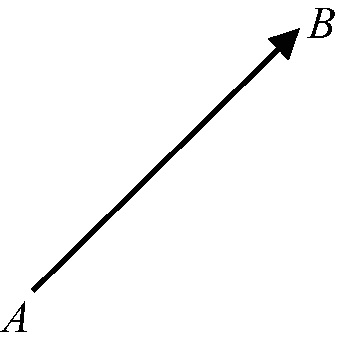
\includegraphics[width = 0.45\linewidth]{pic/C-5/vec}
	\vspace*{-1em}
	\captionof{figure}{向量示意图}
	\label{向量示意图}
\end{minipage}

\defination[自由向量的定义]
在实际研究中,我们只关心向量的方向和大小,称为\highlight{dy}{\index{ZYXL@自由向量}自由向量}。

\defination[向量的夹角定义]
\vspace*{0.5em}

\noindent
\begin{minipage}{0.55\linewidth}
\hspace*{2em} 设有两个非零向量$\boldsymbol{a}$,$\boldsymbol{b}$,任取空间中一点$O$,作$\boldsymbol{OA}=\boldsymbol{a}$,$\boldsymbol{OB}=\boldsymbol{b}$,规定$0\leq \varphi=\angle AOB\leq \pi$,那么$\angle AOB$称为\highlight{dy}{\index{XLDJJ@向量的夹角}向量$\boldsymbol{a}$,$\boldsymbol{b}$的夹角},记作$\langle\boldsymbol{a}$,$\boldsymbol{b}\rangle$或$\langle\boldsymbol{b}$,$\boldsymbol{a}\rangle$,即$\langle\boldsymbol{a}$,$\boldsymbol{b}\rangle=\varphi$.\\
\hspace*{2em} 特别地,如果$\langle\boldsymbol{a}$,$\boldsymbol{b}\rangle=0$或$\pi$,就称向量$\langle\boldsymbol{a},\boldsymbol{b}
\rangle$平行记作$\boldsymbol{a}\parallel\boldsymbol{b}$,当$\boldsymbol{a}$,$\boldsymbol{b}$平移至起点相同的时候,那么$\langle\boldsymbol{a}$,$\boldsymbol{b}\rangle$一定共线。所以,两个平行的向量也称为\highlight{dy}{\index{GXXL@共线向量}共线向量}。
\end{minipage}
\begin{minipage}{0.45\linewidth}
	\centering
	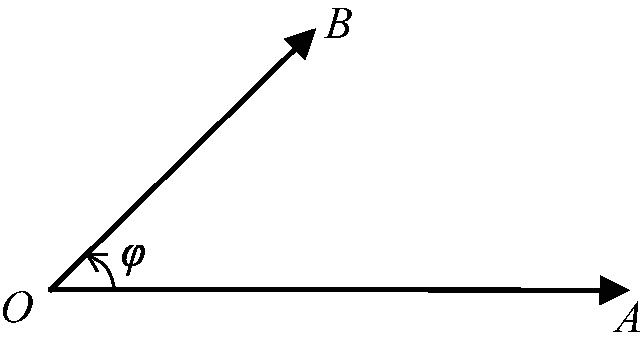
\includegraphics[width = 0.65\linewidth]{pic/C-5/vecang}
	\vspace*{-1em}
	\captionof{figure}{向量的夹角}
	\label{向量的夹角}
\end{minipage}
\vspace*{0.1em}

\noindent \hspace*{2em}如果$\langle\boldsymbol{a}$,$\boldsymbol{b}\rangle$=$\di\frac{\pi}{2}$,就称向量$\boldsymbol{a}$,$\boldsymbol{b}$垂直,记作$\boldsymbol{a}\perp\boldsymbol{b}$.

\warn[\hspace*{2em}零向量与另外的向量的夹角可以任意在{[0,$\pi$]}中取值。因此,可认为零向量与任何向量都平行或垂直]
\defination[向量相等的定义]
如果两个向量$\boldsymbol{a}$,$\boldsymbol{b}$大小和方向都相同,那么向量$\boldsymbol{a}$,$\boldsymbol{b}$是相等的,记作$\boldsymbol{a}=\boldsymbol{b}$.

\newpage

\vspace*{-2em}
\defination[零向量的定义]
零向量的模长为0,方向可以为任意方向。用$\boldsymbol{0}$或者$\vec{0}$表示。
\subsection{向量的线性运算}
向量的线性运算分为加法运算、减法运算以及数乘运算。

\noindent 1.$\,$加法运算法则

\defination[向量的加法]
平行移动使向量$\boldsymbol{a},\boldsymbol{b}$有共同起点,然后由\highlight{dy}{\index{PXSBXFZ@平行四边形法则}平行四边形法则},以$\boldsymbol{a},\boldsymbol{b}$为相邻两边作平行四边形,将平行四边形的对角线所形成的向量定义为\highlight{dy}{\index{HXL@和向量}和向量},如图 \ref{向量加法1} 所示。

\par 或者由\highlight{dy}{\index{SJXFZ@三角形法则}三角形法则},将$\boldsymbol{b}$的起点移至$\boldsymbol{a}$的终点(即首尾相连),然后和向量为$\boldsymbol{a}$的起点指向$\boldsymbol{b}$的终点,如图 \ref{向量加法2} 所示。
\begin{figure}[h]
\centering
\begin{minipage}{0.55\linewidth}
	\centering
	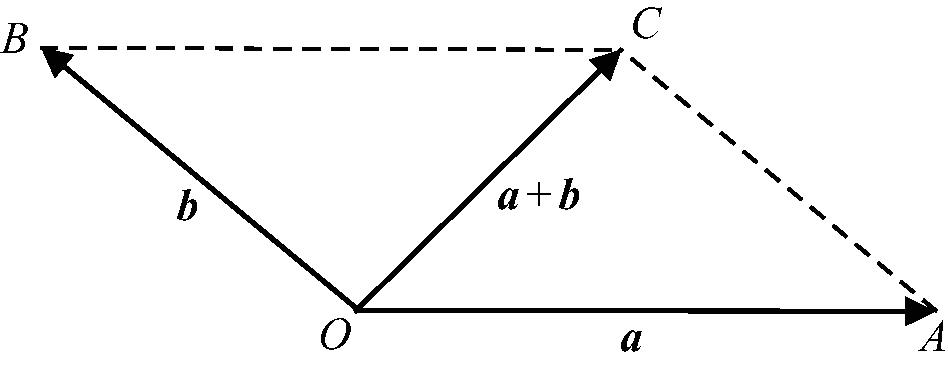
\includegraphics[width = 0.8\linewidth]{pic/C-5/vecadd}
	\vspace*{-0.8em}
	\caption{向量加法(平行四边形法则)}
	\label{向量加法1}
\end{minipage}
\begin{minipage}{0.4\linewidth}
	\centering
	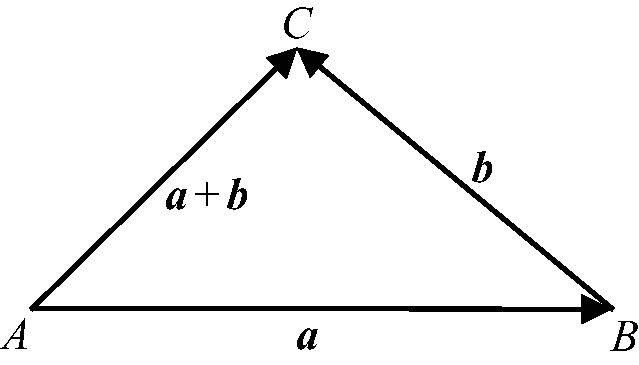
\includegraphics[width = 0.755\linewidth]{pic/C-5/vecadd2}
	\vspace*{-1em}
	\caption{向量加法(三角形法则)}
	\label{向量加法2}
\end{minipage}
\end{figure}
\vspace*{0.5em}

\begin{minipage}{0.55\linewidth}
\noindent \textbf{加法的运算规律:}\\
(1)$\,$ \highlight{dy}{\index{JFJHL@加法交换律}加法交换律}
\vspace*{-0.5em}
\begin{equation}
	\boldsymbol{a}+\boldsymbol{b}=\boldsymbol{b}+\boldsymbol{a} 
\end{equation}
\vspace*{-2em}

(2)$\,$ \highlight{dy}{\index{JFJHL@加法结合律}加法结合律}
\vspace*{-1em}
\begin{equation}
	(\bm{a} + \bm{b}) + \bm{c} = \bm{a} + (\bm{b} + \bm{c})
\end{equation}
\vspace*{-0.3em}
\end{minipage}
\begin{minipage}{0.45\linewidth}
	\centering
	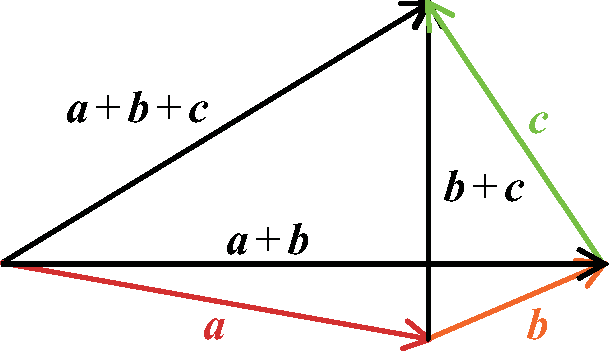
\includegraphics[width = 0.7\linewidth]{pic/C-5/vecadd3}
	\vspace*{-1em}
	\captionof{figure}{向量加法的运算规律}
	\label{向量加法的运算规律}
\end{minipage}
\vspace*{0.5em}

\noindent 2.$\,$减法运算法则\\
\vspace*{-1em}\vspace*{-1em}

\defination[向量的减法]
与向量$\boldsymbol{a}$模长相同而方向相反的向量叫做$\boldsymbol{a}$的\highlight{dy}{\index{FXL@反向量}反向量},记作$-\boldsymbol{a}$,那么\highlight{dy}{\index{XLDC@向量的差}向量$\boldsymbol{b},\boldsymbol{a}$的差}为:
\begin{equation}
	\boldsymbol{b}-\boldsymbol{a}=\boldsymbol{b}+(-\boldsymbol{a})
\end{equation}
可以理解为把向量$-\boldsymbol{a}$加到向量$\boldsymbol{b}$上。(即加法的逆运算,其运算满足加法运算的所有规律),如图 \ref{向量减法1}, \ref{向量减法2} 所示。

\begin{figure}[h]
\centering
\begin{minipage}{0.55\linewidth}
	\centering
	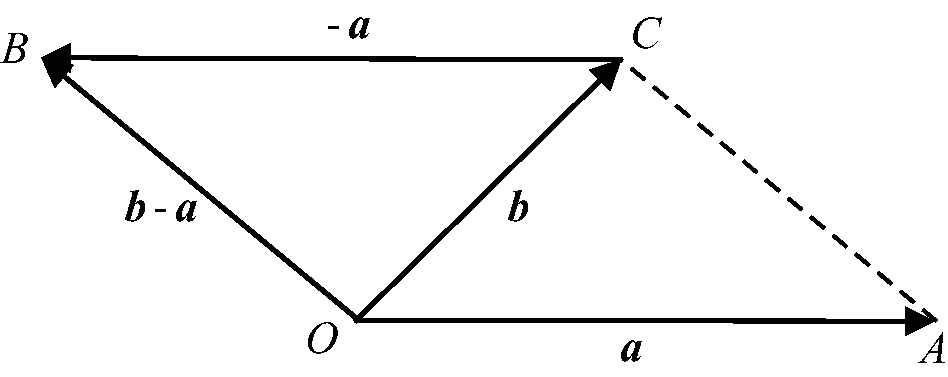
\includegraphics[width = 0.8\linewidth]{pic/C-5/vecdel}
	\vspace*{-1em}
	\caption{向量减法(平行四边形法则)}
	\label{向量减法1}
\end{minipage}
\begin{minipage}{0.4\linewidth}
	\centering
	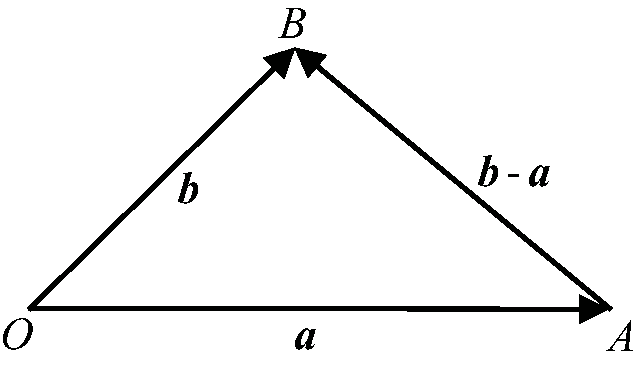
\includegraphics[width = 0.755\linewidth]{pic/C-5/vecdel2}
	\vspace*{-1em}
	\caption{向量减法(三角形法则)}
	\label{向量减法2}
\end{minipage}
\end{figure}

\newpage

\noindent 3.$\,$数乘运算法则

\defination[向量的数乘定义]

向量$\boldsymbol{a}$与实数$\lambda$的乘积记作$\lambda\boldsymbol{a}$,规定$\lambda\boldsymbol{a}$也是一个向量,它的模
\begin{equation}
	|\lambda\boldsymbol{a}|=|\lambda||\boldsymbol{a}|
\end{equation}
它的方向有三种情况:

(1)$\,$ 当$\lambda>0$时,其方向与$\boldsymbol{a}$相同;

(2)$\,$ 当$\lambda<0$时,其方向与$\boldsymbol{a}$相反;

(3)$\,$ 当$\lambda=0$时,$\lambda\boldsymbol{a}$为零向量,这时其方向可以是任意的。\\[0.5em]
\textbf{数乘的运算规律:}

(1)$\,$ \highlight{dy}{\index{SCJHL@数乘交换律}数乘结合律} \qquad
$\lambda(\mu\boldsymbol{a})=\mu(\lambda\boldsymbol{a})=(\lambda\mu)\boldsymbol{a}$

(2)$\,$ \highlight{dy}{\index{SCFPL@数乘分配律}数乘分配律} \qquad
$(\lambda+\mu)\boldsymbol{a}=\lambda\boldsymbol{a}+\mu \boldsymbol{a}$\qquad $\lambda(\boldsymbol{a}+\boldsymbol{b})=\lambda\boldsymbol{a}+\lambda\boldsymbol{b}$


\subsection{向量的内积、外积及混合积}
\noindent1.$\,$向量的内积

\defination[向量的内积定义]

向量$\boldsymbol{a},\boldsymbol{b}$的内积为
\begin{equation}
	\boldsymbol{a}\cdot\boldsymbol{b}=|\boldsymbol{a}||\boldsymbol{b}|\cos\langle\boldsymbol{a},\boldsymbol{b}\rangle
\end{equation}
特别地,当向量$\boldsymbol{a},\boldsymbol{b}$中有一个为零向量,其内积为0.向量的\highlight{dy}{\index{NJ@内积}内积}也称为\highlight{dy}{\index{SLJ@数量积}数量积}或\highlight{dy}{\index{DC@点乘}点乘}。\\
\textbf{点乘的运算规律:}

(1)$\,$\highlight{dy}{\index{JHL@交换律}交换律}\qquad $\boldsymbol{a}\cdot\boldsymbol{b}=\boldsymbol{b}\cdot\boldsymbol{a}$

(2)$\,$\highlight{dy}{\index{YSCDJHL@与数乘的结合律}与数乘的结合律}\qquad
$(\lambda\boldsymbol{a})\cdot\boldsymbol{b}=\lambda(\boldsymbol{a}\cdot\boldsymbol{b})$

(3)$\,$\highlight{dy}{\index{FPL@分配律}分配律}\qquad
$(\boldsymbol{a}+\boldsymbol{b})\cdot\boldsymbol{c}=\boldsymbol{a}\cdot\boldsymbol{c}+\boldsymbol{b}\cdot\boldsymbol{c}$\\[0.5em]
\textbf{内积的重要应用:}
\begin{equation}
	\boldsymbol{a}\perp\boldsymbol{b}\Leftrightarrow \boldsymbol{a}\cdot\boldsymbol{b}=0 
\end{equation}

\noindent 2.$\,$向量的外积

\defination[向量的外积定义]
向量$\boldsymbol{a}$,$\boldsymbol{b}$的外积$\boldsymbol{c}$为
\begin{equation}
	|\boldsymbol{c}|=|\boldsymbol{a}\times\boldsymbol{b}|=|\boldsymbol{a}||\boldsymbol{b}|\sin\langle\boldsymbol{a},\boldsymbol{b}\rangle
\end{equation}
其中外积$\boldsymbol{c}$的方向根据右手法则确定,就是手掌立在$\boldsymbol{a}$,$\boldsymbol{b}$所在平面的向量$\boldsymbol{a}$上,掌心向$\boldsymbol{b}$,那么大拇指方向就是垂直于该平面的方向,即为外积的方向。向量的\highlight{dy}{\index{WJ@外积}外积}也称为\highlight{dy}{\index{XLJ@向量积}向量积}或\highlight{dy}{\index{XLDCC@向量的叉乘}向量的叉乘}。\\

\noindent
\begin{minipage}{0.6\linewidth}
\textbf{外积的几何意义:}
\begin{equation}
	|\boldsymbol{a}\times\boldsymbol{b}|=|\boldsymbol{a}||\boldsymbol{b}|\sin \theta
\end{equation}
其中,$|\boldsymbol{a}\times\boldsymbol{b}|$是以$|\boldsymbol{a}|,|\boldsymbol{b}|$为邻边的平行四边形面积,如图 \ref{向量的外积} 所示。\\
\textbf{外积的运算规律:}\\
\hspace*{2em}(1)\hspace*{0.5em}\highlight{dy}{\index{FJHL@交换律}反交换律}\qquad $\boldsymbol{a}\times\boldsymbol{b}=\boldsymbol{b}\times\boldsymbol{a}$\\
\hspace*{2em}(2)\hspace*{0.5em}\highlight{dy}{\index{FPL@分配律}分配律}\qquad
$(\boldsymbol{a}+\boldsymbol{b})\times\boldsymbol{c}=\boldsymbol{a}\times\boldsymbol{c}+\boldsymbol{b}\times\boldsymbol{c}$\\
\hspace*{2em}(3)\hspace*{0.5em}\highlight{dy}{\index{YSCDJHL@与数乘的结合律}与数乘的结合律}\qquad
$(\lambda\boldsymbol{a})\times\boldsymbol{b}=\boldsymbol{a}\times(\lambda\boldsymbol{b})=\lambda(\boldsymbol{a}\times\boldsymbol{b})$
\end{minipage}
\begin{minipage}{0.4\linewidth}
	\centering
	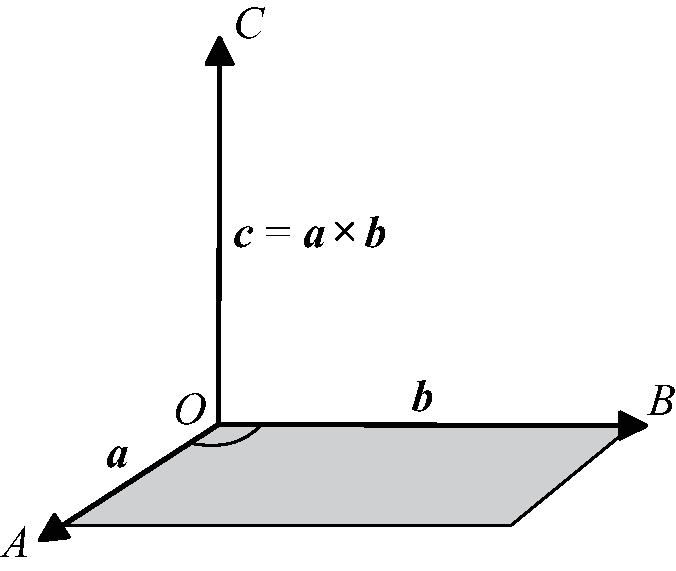
\includegraphics[width = 0.72\linewidth]{pic/C-5/veccross}
	\vspace*{-1em}
	\captionof{figure}{向量的外积}
	\label{向量的外积}
\end{minipage}

\noindent \textbf{外积的重要应用:}
\begin{equation}
	\boldsymbol{a}\parallel\boldsymbol{b}\Leftrightarrow \boldsymbol{a}\times\boldsymbol{b}=0
\end{equation}
3.$\,$向量的混合积\\

\vspace*{-1em}\vspace*{-1em}
\defination[向量混合积的定义] 

\noindent
\begin{minipage}{0.55\linewidth}
\hspace*{2em}设已知三个向量$\boldsymbol{a}$,$\boldsymbol{b}$,$\boldsymbol{c}$,数量$(\boldsymbol{a}\times\boldsymbol{b})\cdot \boldsymbol{c}$称为这三个向量的\highlight{dy}{\index{HHJ@混合积}混合积},记为$[\boldsymbol{a}\,\boldsymbol{b}\,\boldsymbol{c}]$.
\\ 
\textbf{混合积的几何意义:}\\ 
\hspace*{2em} 如图 \ref{向量的混合积} 所示,设非零向量$\boldsymbol{a},\boldsymbol{b},\boldsymbol{c}$,那么记$\boldsymbol{d}=\boldsymbol{a}\times\boldsymbol{b}$,$\boldsymbol{a},\boldsymbol{b},\boldsymbol{c}$构成一个平行六面体,那么将$\boldsymbol{c}$分成与$\boldsymbol{d}$正交与平行的两个分向量$\boldsymbol{c_1},\boldsymbol{c_2}$.\vspace{-0.5em}
\end{minipage}
\begin{minipage}{0.45\linewidth}
	\centering
	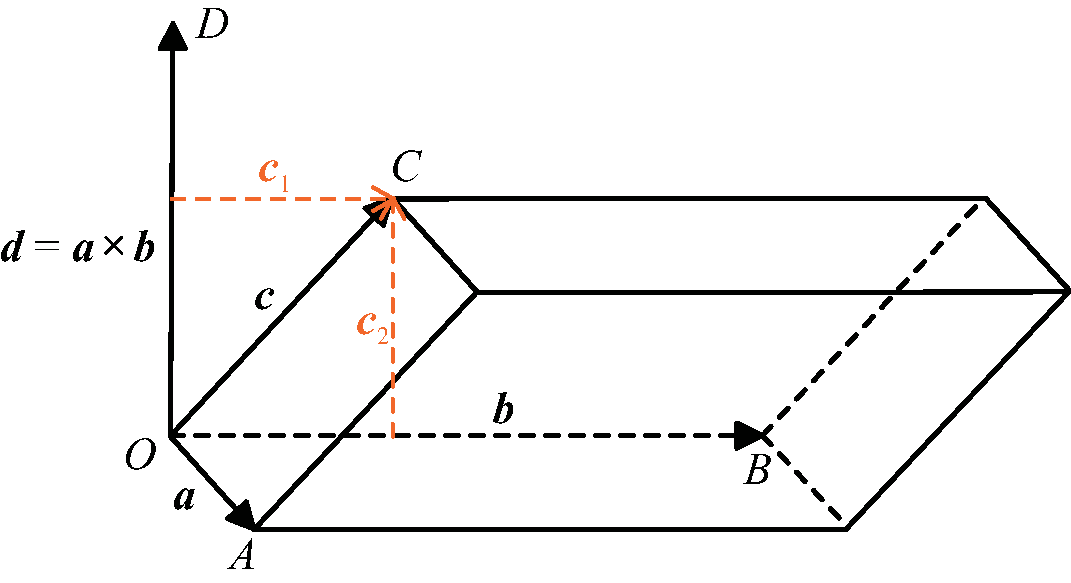
\includegraphics[width = 0.85\linewidth]{pic/C-5/vecfix}
	\vspace*{-1em}
	\captionof{figure}{向量的混合积}
	\label{向量的混合积}
\end{minipage}

\begin{equation}
	\big|[\boldsymbol{a}\,\boldsymbol{b}\,\boldsymbol{c}]\big|=(\boldsymbol{a}\times\boldsymbol{b})\cdot\boldsymbol{c}=\boldsymbol{d}\cdot\boldsymbol{c}=\boldsymbol{d}\cdot(\boldsymbol{c_1}+\boldsymbol{c_2})=\boldsymbol{d}\cdot\boldsymbol{c_2}=|\boldsymbol{d}|\cdot|\boldsymbol{c_2}|=|\boldsymbol{a}\times\boldsymbol{b}|\cdot\boldsymbol{c_2}=S_{\text{底}}\times h=V\vspace{-0.5em}
\end{equation}
也就是说混合积$[\boldsymbol{a},\boldsymbol{b},\boldsymbol{c}]$的绝对值就是这三个向量$\boldsymbol{a},\boldsymbol{b},\boldsymbol{c}$所构成的平行六面体的体积。
\vspace*{0.5em}

\noindent\textbf{混合积的重要应用:}

(1)$\,$求三个向量$\boldsymbol{a},\boldsymbol{b},\boldsymbol{c}$所构成的平行六面体的体积。

(2)$\,$三个向量$\boldsymbol{a},\boldsymbol{b},\boldsymbol{c}$共面$\Leftrightarrow$ $[\boldsymbol{a},\boldsymbol{b},\boldsymbol{c}]=0$.

\section{向量的空间坐标}
\subsection{空间直角坐标系}
\vspace*{-0.5em}
\defination[空间直角坐标系的定义]

\noindent
\begin{minipage}{0.55\linewidth}
\hspace*{2em}空间任意选定一点$O$,过点$O$作三条互相垂直的数轴$Ox,Oy,Oz$,它们都以$O$为原点且具有相同的长度单位。这三条轴分别称作$x$轴(横轴),$y$(纵轴),$z$(竖轴),统称为坐标轴。它们的正方向符合右手规则,即以右手握住$z$轴,当右手的四个手指$x$轴的正向以$90\circ$转向$y$轴正向时,大拇指的指向就是$z$轴的正向。\\
\hspace*{2em} 简单地讲,就是\textbf{一个原点,三个坐标轴,三个坐标面,八个卦限},如图 \ref{空间直角坐标系} 所示,而数组$(x,y,z)$对应空间上的一点坐标。
\end{minipage}
\begin{minipage}{0.45\linewidth}
	\centering
	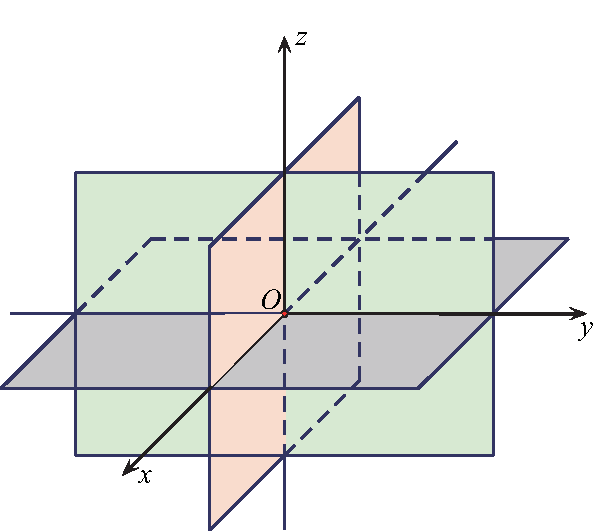
\includegraphics[width = 0.8\linewidth]{pic/C-5/空间坐标}
	\vspace*{-1em}
	\captionof{figure}{空间直角坐标系}
	\label{空间直角坐标系}
\end{minipage}

\subsection{向量的空间坐标的表示与计算}
\vspace*{-0.5em}

\defination[向量的空间坐标定义]
\noindent
\begin{minipage}{0.6\linewidth}
\hspace*{2em}如图 \ref{向量的空间坐标表示} 所示,设向量$\boldsymbol{i},\boldsymbol{j},\boldsymbol{k}$分别为$x$轴,$y$轴,$z$轴的单位向量,那么对于空间点$A(x,y,z)$,$\boldsymbol{OA}$可以表示为
\begin{equation}
	\boldsymbol{OA}=x\boldsymbol{i}+y\boldsymbol{j}+z\boldsymbol{k}
\end{equation}
设$\boldsymbol{r}=\boldsymbol{OA}$,那么我们规定向量$\boldsymbol{r}$的坐标为$(x,y,z)$,记作$\boldsymbol{r}=(x,y,z)$.\\[0.5em]
\textbf{1.$\,$向量的线性运算的坐标表示}\\
\hspace*{2em} 记向量$\boldsymbol{a}=(x_1,y_1,z_1)$,$\boldsymbol{b}=(x_2,y_2,z_2)$,那么
\end{minipage}
\begin{minipage}{0.4\linewidth}
	\centering
	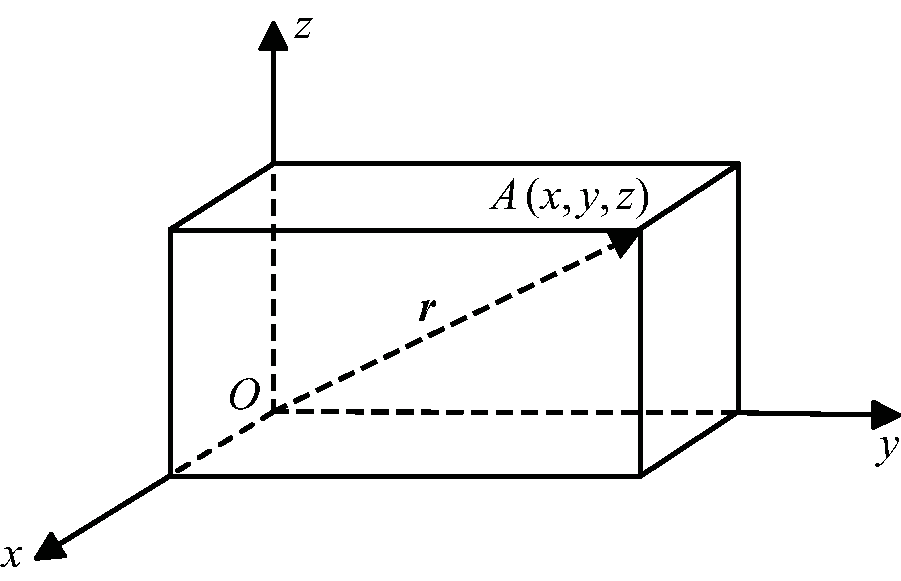
\includegraphics[width = 0.9\linewidth]{pic/C-5/veclinar}
	\vspace*{-1em}
	\captionof{figure}{向量的空间坐标表示}
	\label{向量的空间坐标表示}
\end{minipage}
\vspace*{-0.5em}

(1)$\quad \boldsymbol{a}+\boldsymbol{b}=(x_1+x_2,y_1+y_2,z_1+z_2)$

(2)$\quad \boldsymbol{a}-\boldsymbol{b}=(x_1-x_2,y_1-y_2,z_1-z_2)$

(3)$\quad \lambda \boldsymbol{a}=(\lambda x_1,\lambda y_1,\lambda z_1)$\\[0.5em]
\textbf{2.$\,$向量的内积、外积的坐标表示}

记向量$\boldsymbol{a}=(x_1,y_1,z_1),\,\boldsymbol{b}=(x_2,y_2,z_2)$,那么
\begin{flalign}
\mbox{\textbf{内积:}}\boldsymbol{a}\cdot\boldsymbol{b}=x_1x_2+y_1y_2+z_1z_2
\end{flalign}
特别地,$\boldsymbol{a}^2=\boldsymbol{a}\cdot\boldsymbol{a}=x_1^2+y_1^2+z_1^2$,那么向量$\boldsymbol{a}$的模长为$|\boldsymbol{a}|=\sqrt{\boldsymbol{a}^2}=\sqrt{x_1^2+y_1^2+z_1^2}.$\\[0.5em]
那么由$\boldsymbol{a}\cdot\boldsymbol{b}=|\boldsymbol{a}||\boldsymbol{b}|\cos\langle \boldsymbol{a},\boldsymbol{b}\rangle$,得$\di\cos\langle \boldsymbol{a},\boldsymbol{b}\rangle=\frac{\boldsymbol{a}\cdot\boldsymbol{b}}{|\boldsymbol{a}||\boldsymbol{b}|}=\frac{x_1x_2+y_1y_2+z_1z_2}{\sqrt{x_1^2+y_1^2+z_1^2}\sqrt{x_2^2+y_2^2+z_2^2}}$,那么

\begin{align}
\mbox{\textbf{外积:}}\boldsymbol{a}\times\boldsymbol{b}=(y_1z_2-z_1y_2)\,\boldsymbol{i}+(z_1x_2-x_1z_2)\,\boldsymbol{j}+(x_1y_2-y_1x-2)\,\boldsymbol{k}=
	\begin{bmatrix}
		\boldsymbol{i} & \boldsymbol{j} & \boldsymbol{k}\\
		x_1 & y_1 & z_1\\
		x_2 & y_2 & z_2\\
	\end{bmatrix}
\end{align}
特别地,
\begin{equation}
	\boldsymbol{a}\parallel\boldsymbol{b}\Leftrightarrow \frac{x_1}{y_1}=\frac{y_1}{y-2}=\frac{z_1}{z_2}
\end{equation}
\textbf{混合积:}
\begin{equation*}
	\begin{split}
		\boldsymbol{c}\cdot(\boldsymbol{a}\times\boldsymbol{b})&=(x_0\boldsymbol{i}+y_0\boldsymbol{j}+z_0\boldsymbol{k})	
	\begin{bmatrix}
		\boldsymbol{i} & \boldsymbol{j} & \boldsymbol{k}\\
		x_1 & y_1 & z_1\\
		x_2 & y_2 & z_2\\
	\end{bmatrix}\\[1em]
	&=x_0\boldsymbol{i}
	\begin{bmatrix}
	\boldsymbol{i} & \boldsymbol{j} & \boldsymbol{k}\\
	x_1 & y_1 & z_1\\
	x_2 & y_2 & z_2\\
\end{bmatrix}+y_0\boldsymbol{j}	
\begin{bmatrix}
\boldsymbol{i} & \boldsymbol{j} & \boldsymbol{k}\\
x_1 & y_1 & z_1\\
x_2 & y_2 & z_2\\
\end{bmatrix}+z_0\boldsymbol{k}	
\begin{bmatrix}
\boldsymbol{i} & \boldsymbol{j} & \boldsymbol{k}\\
x_1 & y_1 & z_1\\
x_2 & y_2 & z_2\\
\end{bmatrix}\\[1em]
	&=\begin{bmatrix}
		x_0\boldsymbol{i}\cdot\boldsymbol{i} & x_0\boldsymbol{i}\cdot\boldsymbol{j} & x_0\boldsymbol{i}\cdot\boldsymbol{k}\\
	x_1 & y_1 & z_1\\
	x_2 & y_2 & z_2\\
	\end{bmatrix}+
\begin{bmatrix}
	y_0\boldsymbol{j}\cdot\boldsymbol{i} & y_0\boldsymbol{j}\cdot\boldsymbol{j} & y_0\boldsymbol{j}\cdot\boldsymbol{k}\\
	x_1 & y_1 & z_1\\
	x_2 & y_2 & z_2\\
\end{bmatrix}+
\begin{bmatrix}
	z_0\boldsymbol{k}\cdot\boldsymbol{i} & z_0\boldsymbol{k}\cdot\boldsymbol{j} & z_0\boldsymbol{k}\cdot\boldsymbol{k}\\
	x_1 & y_1 & z_1\\
	x_2 & y_2 & z_2\\
\end{bmatrix}=
\begin{bmatrix}
	x_0 & y_0 & z_0\\
	x_1 & y_1 & z_1\\
	x_2 & y_2 & z_2\\
\end{bmatrix}
	\end{split}
\end{equation*}
注:$\boldsymbol{i}\cdot\boldsymbol{i}=1,\, \boldsymbol{i}\cdot\boldsymbol{j}=0,\, \boldsymbol{i}\cdot\boldsymbol{k}=0$其余类似可得,本质上就是利用三个坐标轴上的单位向量相乘。



\subsection{方向角与方向余弦}
\vspace*{-0.5em}

\defination[方向角与方向余弦]
\vspace*{0.5em}
\noindent
\begin{minipage}{0.55\linewidth}
\hspace*{2em}如图 \ref{向量的方向角} 所示,记非零向量$\boldsymbol{r}$与三条坐标轴$(x,y,z)$的夹角$\alpha,\beta,\gamma$为向量$\boldsymbol{r}$的方向角。设$\boldsymbol{r}=\boldsymbol{OA}=(x,y,z)$,则
\begin{equation}
	\cos \alpha=\frac{x}{|OA|}=\frac{x}{\boldsymbol{|r|}}=\frac{x}{\sqrt{x^2+y^2+z^2}}
\end{equation}
\begin{equation}
	\cos \beta=\frac{y}{|OA|}=\frac{y}{\boldsymbol{|r|}}=\frac{y}{\sqrt{x^2+y^2+z^2}}
\end{equation}
\begin{equation}
	\cos \gamma=\frac{z}{|OA|}=\frac{z}{\boldsymbol{|r|}}=\frac{z}{\sqrt{x^2+y^2+z^2}}
\end{equation}
那么,向量$\boldsymbol{r}$方向上的方向向量可以表示成:
\end{minipage}
\begin{minipage}{0.45\linewidth}
	\centering
	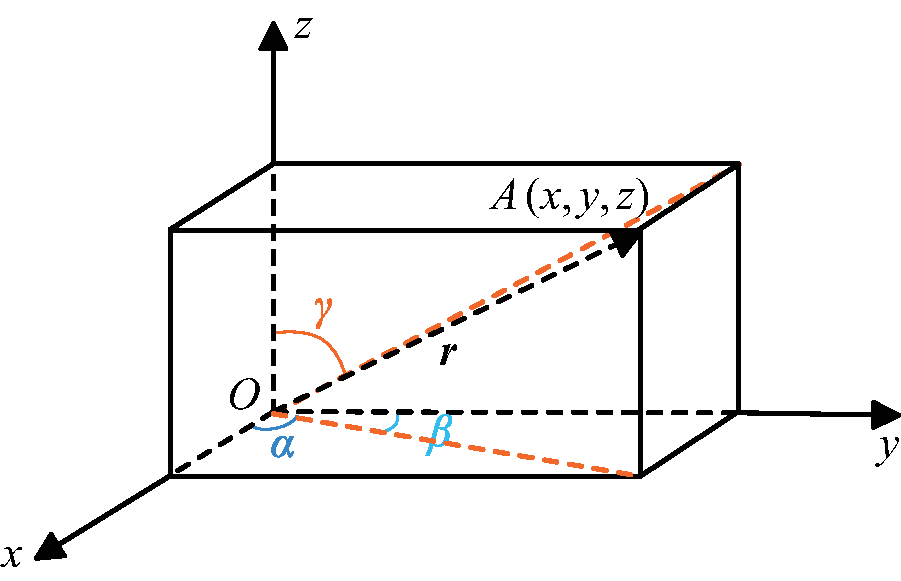
\includegraphics[width = 0.85\linewidth]{pic/C-5/vesang3}
	\vspace*{-1em}
	\captionof{figure}{向量的方向角}
	\label{向量的方向角}
\end{minipage}

\begin{equation}
	\boldsymbol{e_r}=(\cos \alpha,\cos \beta,\cos \gamma)=\bigg(\frac{x}{|\boldsymbol{r}|},\frac{y}{|\boldsymbol{r}|},\frac{z}{|\boldsymbol{r}|}\bigg)=\frac{1}{|\boldsymbol{r}|}(x,y,z)=\frac{\boldsymbol{r}}{|\boldsymbol{r}|}
\end{equation}
\section{空间平面与空间直线}
\subsection{平面的方程}
平面的方程一般有四种表达方式:点法式、一般式、三点式、截距式。
\vspace*{1em}

\noindent
\begin{minipage}{0.6\linewidth}
\textbf{1.$\,$平面的点法式方程}\\ 
\hspace*{2em}如图 \ref{平面的点法式方程} 所示,设平面的法向量$\boldsymbol{n}$(即垂直于平面的向量)的坐标为$(A,B,C)$ $(A,B,C$不全为$0)$。设点$P_0(x_0,y_0,z_0)$在平面上,那么平面上任意一点$P(x,y,z)$满足:
\begin{equation}
	\nonumber
	\boldsymbol{n}\cdot\boldsymbol{PP_0}=0
\end{equation}
\end{minipage}
\begin{minipage}{0.4\linewidth}
	\centering
	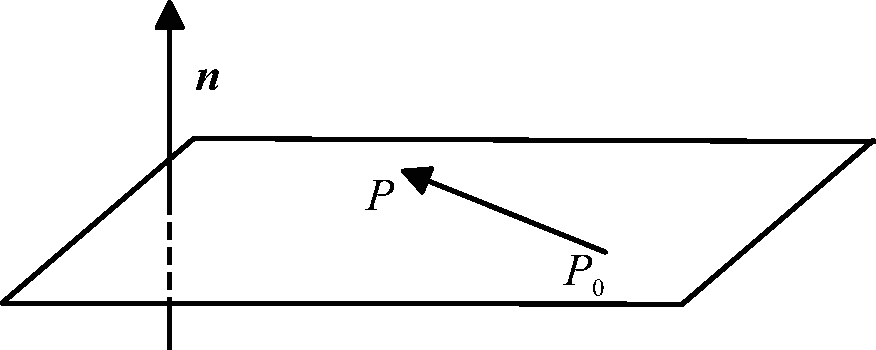
\includegraphics[width = 0.9\linewidth]{pic/C-5/plane1}
	\vspace*{-1em}
	\captionof{figure}{平面的点法式方程}
	\label{平面的点法式方程}
\end{minipage}

\noindent 即
\begin{equation}
	A(x-x_0)+B(y-y_0)+C(z-z_0)=0
	\end{equation}
同样地,如果空间中任何一点$P(x,y,z)$满足这个方程,那么这个点一定在平面上。
\\这个方程是由平面的一个法向量及平面上一已知点的坐标确定的,故通常称为\highlight{dy}{\index{PMDDFSFC@平面的点法式方程}平面的点法式方程}。\\[1em]
\textbf{2.$\,$平面的一般式方程}
\par 我们将点法式方程进一步化简,得:
\begin{equation}
	A(x-x_0)+B(y-y_0)+C(z-z_0)=0\Leftrightarrow Ax+By+Cz-Ax_0-By_0-Cz_0=0
	\label{equ:5.16}
\end{equation}
设式\eqref{equ:5.16}中,$D=-Ax_0-By_0-Cz_0$.上式变为:
\begin{equation}
	Ax+By+Cz+D=0
\end{equation}
那么,式\eqref{equ:5.16}称为\highlight{dy}{\index{PMDYBSFC@平面的一般式方程}平面的一般式方程}。\\

\noindent
\begin{minipage}{0.6\linewidth}
\textbf{3.$\,$平面的三点式方程}\\
\hspace*{2em}如图 \ref{平面的三点式方程} 所示,已知平面上的三点$P_1(x_1,y_1,z_1), P_2(x_2,y_2,z_2),$ $P_3(x_3,y_3,z_3)$,要使这三点能够唯一地确定一个平面,那么这三个点必然不共线。即$\boldsymbol{P_1P_2}\times\boldsymbol{P_1P_3}\neq 0$。那么,平面上任意一点必满足:
\end{minipage}
\begin{minipage}{0.4\linewidth}
	\centering
	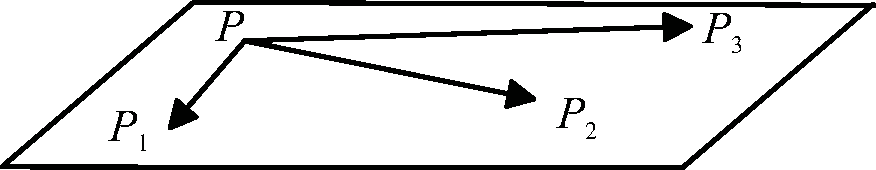
\includegraphics[width = 0.85\linewidth]{pic/C-5/plane2}
	\vspace*{-1em}
	\captionof{figure}{平面的三点式方程}
	\label{平面的三点式方程}
\end{minipage}
\begin{equation}
	\boldsymbol{P_1P}\cdot(\boldsymbol{P_1P_2}\times\boldsymbol{P_1P_3})=0
\end{equation}
即\begin{equation}
	\boldsymbol{P_1P}\cdot(\boldsymbol{P_1P_2}\times\boldsymbol{P_1P_3})=(x-x_1,y-y_1,z-z_1)\cdot
	\begin{vmatrix}
		\boldsymbol{i} & \boldsymbol{j} & \boldsymbol{k}\\
		x_2-x_1 & y_2-y_1 & z_2-z_1\\
		x_3-x_1 & y_3-y_1 & z_3-z_1\\
	\end{vmatrix}=
\begin{vmatrix}
	x-x_1 & y-y_1 & z-z_1\\
	x_2-x_1 & y_2-y_1 & z_2-z_1\\
	x_3-x_1 & y_3-y_1 & z_3-z_1\\
\end{vmatrix}=0
\end{equation}
即\begin{equation}
	\begin{vmatrix}
		x-x_1 & y-y_1 & z-z_1\\
		x_2-x_1 & y_2-y_1 & z_2-z_1\\
		x_3-x_1 & y_3-y_1 & z_3-z_1\\
	\end{vmatrix}=0
\label{equ:5-20}
\end{equation}
那么,式\eqref{equ:5-20}称为\highlight{dy}{\index{PMDSDSFC@平面的三点式方程}平面的三点式方程}。\\[1em]
\textbf{4.$\,$平面的截距式方程}
\par 我们将平面的一般方程$Ax+By+Cz+D=0$进一步变形,当$A,B,C,D\neq0$时,两边同时除以$-D$,得
\begin{equation}
	\displaystyle \frac{x}{-\frac{D}{A}}+\frac{y}{-\frac{D}{B}}+\frac{z}{-\frac{D}{C}}
=1\end{equation}
这个方程称为\highlight{dy}{\index{PMDJJSFC@平面的截距式方程}平面的截距式方程},如图 \ref{平面的截距式方程} 所示。从中也比较容易看出平面与截距的关系。\\

\vspace*{-1em}
\noindent
\begin{minipage}{0.6\linewidth}
\hspace*{2em}(1) \hspace*{0.5em}当$D=0$时,说明平面一定过原点。\\
\hspace*{2em}(2) \hspace*{0.5em}当$A=0$时,平面$By+Cz+D=0$与$x$轴平行。\\
\hspace*{2em}(3) \hspace*{0.5em}当$B=0$时,平面$Ax+Cz+D=0$与$y$轴平行。\\
\hspace*{2em}(4) \hspace*{0.5em}当$C=0$时,平面$Ax+By+D=0$与$z$轴平行。\\
\hspace*{2em}(5) \hspace*{0.5em}当$A,B=0$时,平面$Cz+D=0$与平面$Oxy$轴平行。\\
\hspace*{2em}(6) \hspace*{0.5em}当$B,C=0$时,平面$Ax=0$与平面$Oyz$轴平行。\\
\hspace*{2em}(7) \hspace*{0.5em}当$A,C=0$时,平面$By=0$与平面$Oxz$轴平行。\\
\end{minipage}
\begin{minipage}{0.4\linewidth}
	\centering
	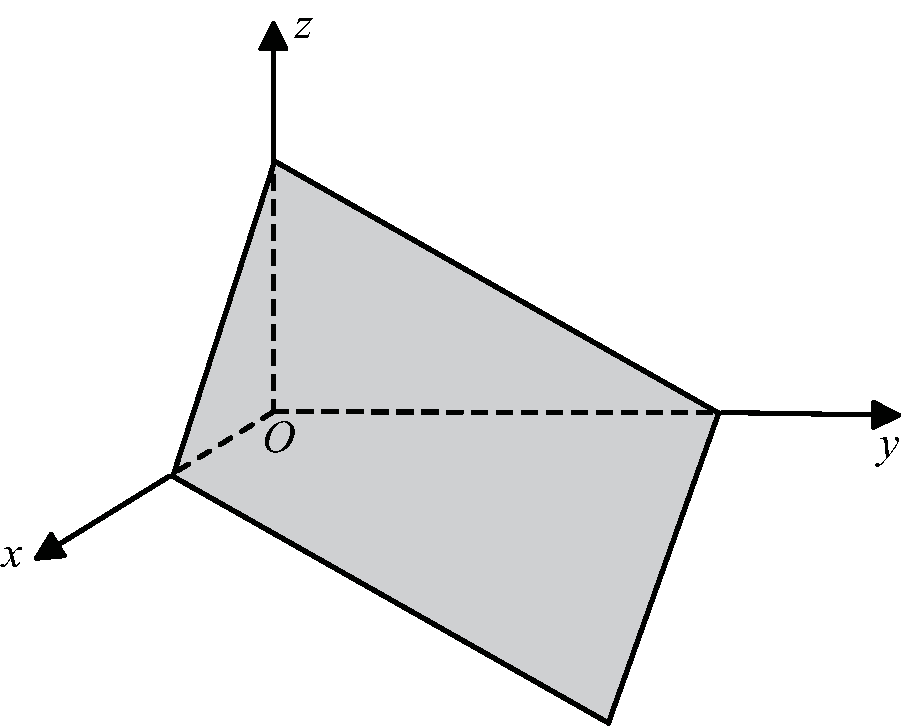
\includegraphics[width = 0.8\linewidth]{pic/C-5/plane3}
	\vspace*{-1em}
	\captionof{figure}{平面的截距式方程}
	\label{平面的截距式方程}
\end{minipage}
\textbf{5.$\,$平面的方程总结}
\par 我们通过对比二维直线的表达式和三维平面的表达式来更好地理解和记忆三维平面方程。
\begin{table}[h]
	\centering
	\setlength{\tabcolsep}{10mm}{
	\begin{tabular}{ccc}
		\toprule[1.5pt]
		方程类型 & 二维直线表达式 & 三维平面表达式\\
		\midrule[0.7pt]
		点法式 & $A(x-x_0)+B(y-y_0)=0$ & $A(x-x_0)+B(y-y_0)+C(z-z_0)=0$\\[0.5em]
		一般式 & $Ax+By+C=0$ & $Ax+By+Cz+D=0$\\[0.5em]
		截距式 & $\displaystyle \frac{x}{a}+\frac{y}{b}=1$ & $\displaystyle \frac{x}{  -\frac{D}{A}}+\frac{y}{-\frac{D}{B}}+\frac{z}{-\frac{D}{C}}=1$\\[1.2em]
		(两)三点式 & $\displaystyle y=kx+b,k=\frac{y_2-y_1}{x_2-x_1}$ & $\begin{vmatrix}
				x-x_1 & y-y_1 & z-z_1\\
			x_2-x_1 & y_2-y_1 & z_2-z_1\\
			x_3-x_1 & y_3-y_1 & z_3-z_1\\
		\end{vmatrix}=0$\\
		& & \\[-1.2em]
		\bottomrule[1.5pt]
	\end{tabular}
}
\end{table}
\vspace*{-0.5em}

\subsection{直线的方程}
直线的方程一般有三种表示方式:一般方程(两面式)、参数方程、标准方程。\\[0.5em]
\textbf{1.$\,$直线的点法式方程}
\par 在空间中,直线一般是由两个平面相交而得到的交线,因此,直线可以用两个平面的方程联立得到。

\noindent
\begin{minipage}{0.6\linewidth}
 设两个相交平面为:
\begin{equation*}
	\begin{split}
	\Pi_1:A_1x+B_1y+C_1z+D_1=0\\
	\Pi_2: A_2x+B_2y+C_2z+D_2=0
	\end{split}
\end{equation*}
联立得,
\begin{equation}
	L:\begin{cases}
	\, A_1x+B_1y+C_1z+D_1=0\\
	\, 	A_2x+B_2y+C_2z+D_2=0\\
		\end{cases}
	\label{equ:5.22}
\end{equation}
那么式\eqref{equ:5.22}就称为\highlight{dy}{\index{ZXDLMDFCHYBFC@直线的两面式方程或一般方程}直线的两面式方程或一般方程}。
\vspace*{0.5em}
\end{minipage}
\begin{minipage}{0.4\linewidth}
	\centering
	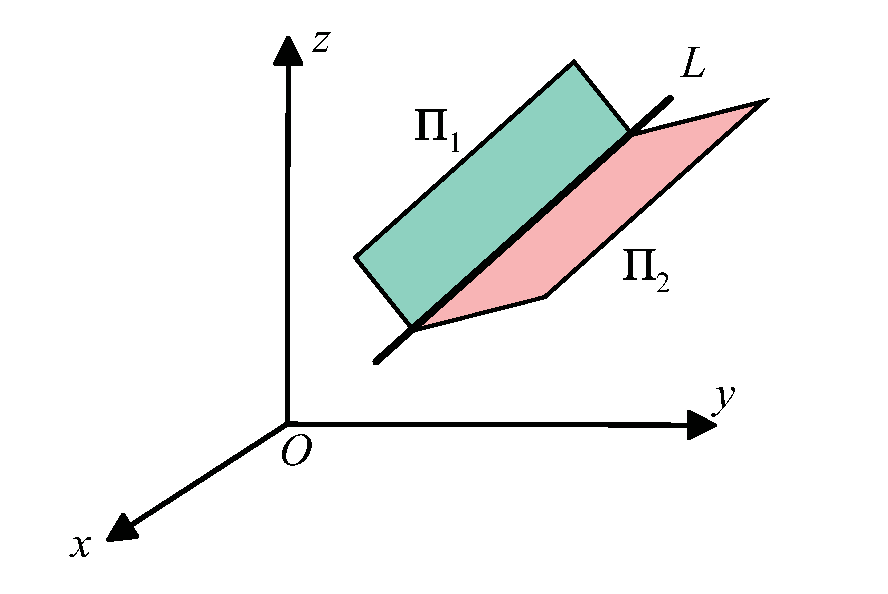
\includegraphics[width = \linewidth]{pic/C-5/line}
	\vspace*{-3em}
	\captionof{figure}{向量的点法式方程}
	\label{直线的点法式方程}
\end{minipage}
\vspace*{0.5em}

\noindent \textbf{2.$\,$直线的参数方程}
\par 已知直线的一点$P_0(x_0,y_0,z_0)$,且直线的非零方向向量为$\boldsymbol{e}=(a,b,c)$,那么就存在一个实数$t$,使得直线上任意一点$P$都满足:
\begin{equation}
	\boldsymbol{P_0P}=t\boldsymbol{e}(-\infty<t<+\infty)
\end{equation}
即
\begin{equation}
	\begin{cases}
		\, x-x_0=ta\\
		\, y-y_0-tb\\
		\, z-z_0=tc
	\end{cases}
(-\infty<t<+\infty)
\label{equ:5.23}
\end{equation}
那么式\eqref{equ:5.23}就称为\highlight{dy}{\index{ZXDCSFC@直线的参数方程}直线的参数方程}。\\[1em]
\textbf{3.$\,$直线的标准方程}
\par 在直线的参数方程ref{equ:5.23}的基础上进一步消去参数,得
\begin{equation}
	\frac{x-x_1}{a}=\frac{y-y_1}{b}=\frac{z-z_1}{c}
\label{equ:5.24}
\end{equation}
那么式\eqref{equ:5.24}就称为\highlight{dy}{\index{ZXDBZFC@直线的标准方程}直线的标准方程}。上述的写法只是一个形式上的写法,实际上完整的式子应该为:
\begin{equation}
	\begin{cases}
		\, a(y-y_0)-b(x-x_0)=0\\
		\, a(z-z_0)-c(x-x_0)=0\\
	\end{cases}
\end{equation}
这时就不需要对$a,b,c$是不是0进行分类讨论。\\[1em]
\textbf{4*.$\,$平面束方程}
\par 设直线$L$由方程组:
\begin{equation}
	\begin{cases}
\, A_1x+B_1y+C_1z+D_1=0\\
\, A_2x+B_2y+C_2z+D_2=0\\
\end{cases}
\end{equation}
确定。其中$A_1,B_1,C_1$与$A_2,B_2,C_2$不成比例。(目的是使两个平面不平行)那么我们建立三元一次方程
\begin{equation}
	A_1x+B_1y+C_1z+D_1+\lambda(A_2x+B_2y+C_2z)+D_2=0
\label{equ:5-41}	
\end{equation}
其中$\lambda$为任意常数。进一步化简,可得
\begin{equation}
	(A_1+\lambda A_1)x+(B_1+\lambda B_2)y+(C_1+\lambda C_2Z)+(D_1+D_2)=0
\end{equation}
\par 由于$A_1,B-1,C_1$与$A_2,B_2,C_2$不成比例,$(A_1+\lambda A_1),(B_1+\lambda B_2),(C_1+\lambda C_2Z),(D_1+D_2)$都部为0.那么上述方程代表的就是一个平面,而由于$\lambda$不确定,而且直线$L$必定是这个方程的解,那么方程\eqref{equ:5-41}就代表着所有通过定直线$L$的平面,称为通过直线$L$的\highlight{dy}{\index{PMSDFC@平面束的方程}平面束的方程}。

\noindent
\begin{minipage}{0.6\linewidth}
\subsection{平面与直线的夹角问题}
\textbf{1.$\,$平面与平面的夹角}\\[0.5em]
\hspace*{2em} 已知两个平面$\Pi_1,\Pi_2$:
\begin{equation*}
	\begin{split}
		\Pi_1:A_1x+B_1y+C_1z+D_1=0\\
		\Pi_2: A_2x+B_2y+C_2z+D_2=0
	\end{split}
\end{equation*}
\end{minipage}
\begin{minipage}{0.4\linewidth}
	\centering
	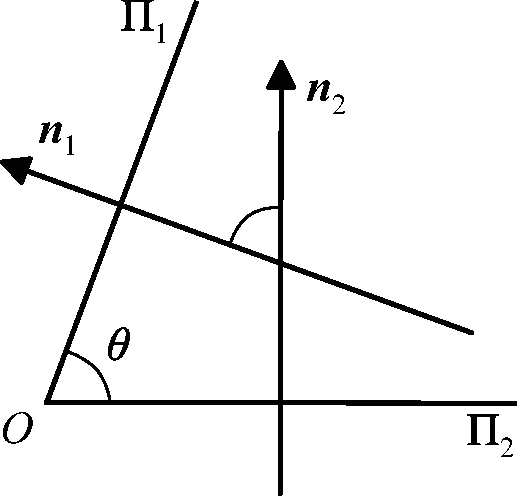
\includegraphics[width = 0.55\linewidth]{pic/C-5/planeang}
	\vspace*{-1em}
	\captionof{figure}{平面与平面的夹角}
	\label{平面与皮昂面的夹角}
\end{minipage}

\noindent 那么它们的夹角$\theta$的余弦值为:
\begin{equation}
	\cos \theta=\cos\langle \boldsymbol{n_1},\boldsymbol{n_2}\rangle =\frac{\boldsymbol{n_1}\cdot\boldsymbol{n_2}}{|\boldsymbol{n_1}||\boldsymbol{n_2}|}=\frac{|A_1A_2+B_1B_2+C_1C_2|}{\sqrt{A_1^2+B_1^2+C_1^2}\cdot\sqrt{A_2^2+B_2^2+C_2^2}}
\end{equation}
那么,我们可以通过这个式子来判断平面之间的关系:

(1)$\hspace*{0.5em} \Pi_1\perp \Pi_2 \Leftrightarrow  A_1A_2+B_1B_2+C_1C_2=0$
\vspace*{0.5em}

\noindent
\begin{minipage}{0.7\linewidth}
\hspace*{2em}(2)$\hspace*{0.5em} \Pi_1\parallel \Pi_2 \Leftrightarrow \displaystyle \frac{A_1}{A_2}=\frac{B_1}{B_2}=\frac{C_1}{C_2} $\vspace*{-0.5em}\\

\textbf{2.$\,$直线与直线的夹角}\\
\hspace*{2em} 如图 \ref{直线间的夹角} 所示,已知两条直线$L_1,L_2$:
\begin{equation}
	L_1: \frac{x-x_1}{m_1}=\frac{y-y_1}{n_1}=\frac{z-z_1}{p_1}
\end{equation}
\begin{equation}
	L_2:\frac{x-x_2}{m_2}=\frac{y-y_2}{n_2}=\frac{z-z_2}{p_2}
\end{equation}
那么它们的夹角$\theta$的余弦值为:
\end{minipage}
\begin{minipage}{0.35\linewidth}
	\centering
	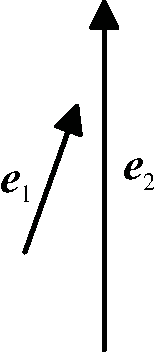
\includegraphics[width = 0.25\linewidth]{pic/C-5/lineang}
	\vspace*{-1em}
	\captionof{figure}{直线间的夹角}
	\label{直线间的夹角}
\end{minipage}

\begin{equation}
\cos\langle L_1,L_2\rangle =\cos \langle \boldsymbol{e_1},\boldsymbol{e_2}\rangle =\frac{\boldsymbol{e_1}\cdot\boldsymbol{e_2}}{|\boldsymbol{e_1}||\boldsymbol{e_2}|}=\frac{|m_1m_2+n_1n_2+p_1p_2|}{\sqrt{m_1^2+n_1^2+p_1^2}\sqrt{m_2^2+n_2^2+p_2^2}}
\end{equation}
那么,我们可以通过这个式子来判断直线之间的关系:
\vspace*{1em}

\noindent
\begin{minipage}{0.6\linewidth}
\hspace*{2em}(1)$\hspace*{0.5em} L_1\perp L_2 \Leftrightarrow  m_1m_2+n_1n_2+p_1p_2=0$
\vspace*{0.5em}

\hspace*{2em}(2)$\hspace*{0.5em} L_1\parallel L_2 \Leftrightarrow \displaystyle \frac{m_1}{m_2}=\frac{n_1}{n_2}=\frac{p_1}{p_2} $
\vspace*{1em}

\textbf{3.$\,$直线与平面的夹角}

\hspace*{2em}如图 \ref{直线与平面的夹角} 所示,已知直线$L$和平面$\Pi$:
\begin{equation}
	\nonumber
	L:\frac{x-x_0}{m}=\frac{y-y_0}{n}=\frac{z-z_0}{p}
\end{equation}
\begin{equation}
	\nonumber
	\Pi:Ax+By+Cz+D=0
\end{equation}
那么它们的夹角$\theta$的正弦值为:
\end{minipage}
\begin{minipage}{0.4\linewidth}
	\centering
	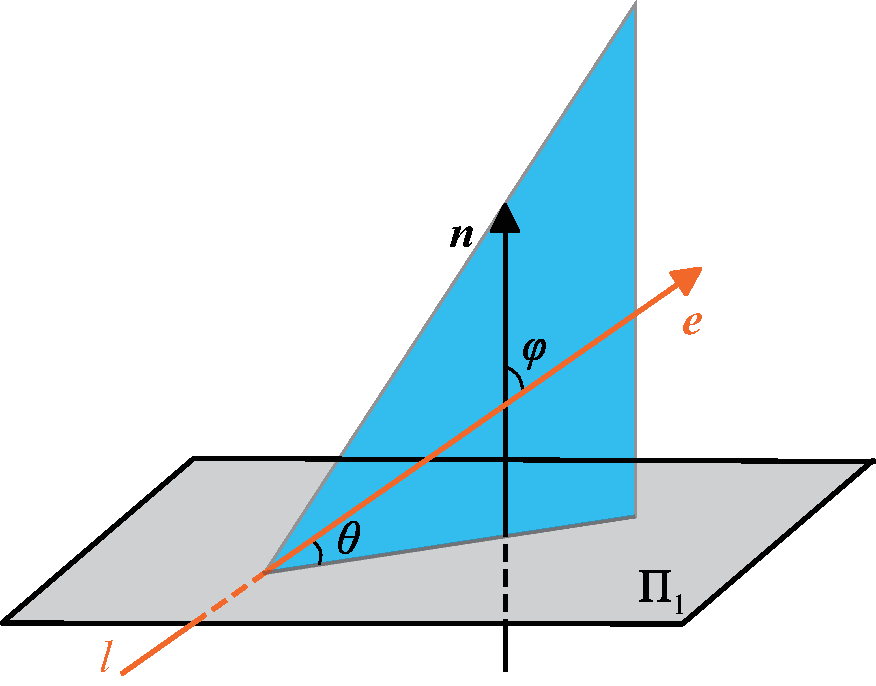
\includegraphics[width = 0.8\linewidth]{pic/C-5/planelineang}
	\vspace*{-1em}
	\captionof{figure}{直线与平面的夹角}
	\label{直线与平面的夹角}
\end{minipage}

\begin{equation}
	\sin \varphi =\cos\bigg( \frac{\pi}{2}-\varphi\bigg)=\cos \theta=\cos \langle \boldsymbol{e},\boldsymbol{n}\rangle =\frac{|Am+Bn+Cp|}{\sqrt{A^2+B^2+C^2}\cdot\sqrt{m^2+n^2+p^2}}
\end{equation}
那么,我们可以通过这个式子来判断直线与平面之间的关系:

(1)$\hspace*{0.5em} L\perp \Pi \Leftrightarrow  Am+Bn+Cp=0$
\vspace*{0.5em}

(2)$\hspace*{0.5em} L\parallel \Pi \Leftrightarrow \displaystyle \frac{A}{m}=\frac{B}{n}=\frac{C}{p} $



\newpage
\subsection{平面与直线的距离问题}

\noindent \textbf{1.$\,$点与点的距离}
	
设点$M_1(x_1,y_1,z_1),M_2(x_2,y_2,z_2)$,那么两点间距离为:
\begin{equation}
	|M_1M_2|=\sqrt{(x_2-x_1)^2+(y_2-y_1)^2+(z_2-z_1)^2}
\end{equation}

\noindent
\begin{minipage}{0.6\linewidth}
\textbf{2.$\,$点到平面的距离}

\hspace*{2em}如图 \ref{点到平面的距离} 所示,已知一个平面$Ax+By+Cz+D=0(A,B,C$不全为0)和平面外一点$P_1(x_1,y_1,z_1)$,取平面内一点$P_0(x_0,y_0,z_0)$,那么点$P_1$到平面的距离为:
\end{minipage}
\begin{minipage}{0.4\linewidth}
	\centering
	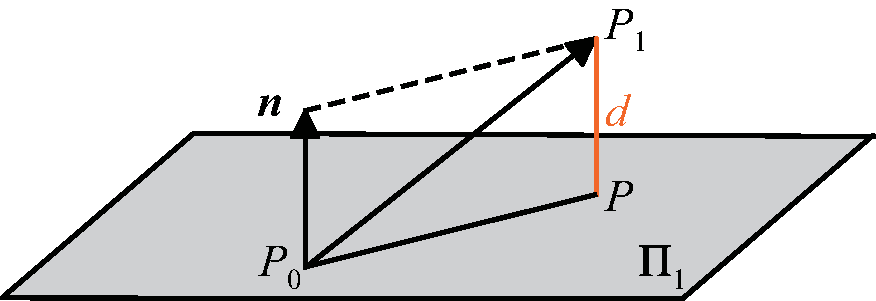
\includegraphics[width = 0.8\linewidth]{pic/C-5/planed}
	\vspace*{-1em}
	\captionof{figure}{点到平面的距离}
	\label{点到平面的距离}
\end{minipage}
\vspace*{-0.5em}

\begin{equation}
	d=|\boldsymbol{P_0P_1}|\cos \langle \boldsymbol{P_0P_1}\cdot \boldsymbol{n} \rangle|=\frac{\boldsymbol{P_0P_1}\cdot \boldsymbol{n}}{\boldsymbol{n}}=\frac{|A(x_1-x_0)+B(y_1-y_0)+C(z_1-z_0)|}{\sqrt{A^2+B^2+C^2}}
\end{equation}
又$P_0$在平面$Ax+By+Cz+D=0$上,\\
所以,$D=-Ax_0-By_0-Cz_0$,即
\begin{equation}
	d=\frac{|A(x_1-x_0)+B(y_1-y_0)+C(z_1-z_0)|}{\sqrt{A^2+B^2+C^2}}=\frac{|Ax_1+By_1+Cz_1+D|}{\sqrt{A^2+B^2+C^2}}
\end{equation}
\vspace*{-2.5em}
\summarize[\hspace*{2em}联想二维空间中点到直线的距离公式进行记忆:
\begin{equation}
	d=\frac{|Ax_1+By_1+C|}{\sqrt{A^2+B^2}}
	\end{equation}]
	
\noindent \textbf{3.$\,$直线到平面的距离/平面到平面的距离}

我们只需要在直线或者平面上任取一个点,就变成点到平面的距离问题。
\vspace*{1em}

\noindent
\begin{minipage}{0.65\linewidth}
	\noindent \textbf{4.$\,$点到直线的距离}
 \\ \hspace*{2em}如图 \ref{点到空间直线的距离} 所示,已知一条直线
\begin{equation}
	L:\frac{x-x_0}{m}=\frac{y-y_0}{n}=\frac{z-z_0}{p}
\end{equation}
和直线外一点$P_1(x_1,y_1,z_1)$,过点$P_1$作平面垂直于直线$L$,交于点$P$,那么平面的方程为:
\begin{equation}
	m(x-x_1)+n(y-y_1)+p(z-z_1)=0
\end{equation}
\end{minipage}
\begin{minipage}{0.35\linewidth}
	\centering
	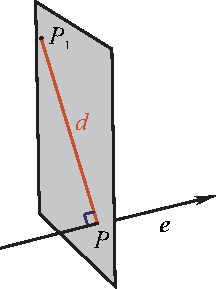
\includegraphics[width = 0.55\linewidth]{pic/C-5/linepd}
	\vspace*{-1em}
	\captionof{figure}{点到空间直线的距离}
	\label{点到空间直线的距离}
\end{minipage}

\vspace*{0.5em}
\noindent 那么联立平面与直线方程,得
\begin{equation}
	\begin{cases}
		\, m(x-x_1)+n(y-y_1)+p(z-z_1)=0\\
		\, m(y-y_0)-n(x-x_0)=0\\
		\, m(z-z_0)-p(x-x_0)=0\\
	\end{cases}
\end{equation}
然后解出$P$点的坐标,用两点间的距离公式计算出$d$的值。\\[1em]
\textbf{5.$\,$平行直线的距离}
\par 我们只需要在任意一条直线上任取一个点,就变成点到直线的距离问题。



\newpage
\section{空间曲面}
\subsection{旋转曲面}

\vspace*{-0.5em}
\defination[旋转曲面]
\vspace*{0.2em}

\noindent
\begin{minipage}{0.65\linewidth}
\hspace*{2em}以一条平面曲线绕其平面上的一条直线旋转一周所成的曲面叫做\highlight{dy}{\index{XZQM@旋转曲面}旋转曲面},旋转曲线和定直线依次叫做旋转曲面的\highlight{dy}{\index{MX@母线}母线}和\highlight{dy}{\index{Z@轴}轴},如图 \ref{旋转曲面} 所示。\\
\hspace*{2em}设在$yOz$坐标面上有一已知曲面$C$,它的方程为
\begin{equation}
	f(y,z)=0
\end{equation}
把这条曲线绕$z$轴旋转一周,就得到一个以$z$轴为旋转轴的旋转曲面,它的方程可以用以下的方法求解。\\
\hspace*{2em}设$P_0(0,y_0,z_0)$为曲线$C$上任意一点,则有
\end{minipage}
\begin{minipage}{0.35\linewidth}
	\centering
	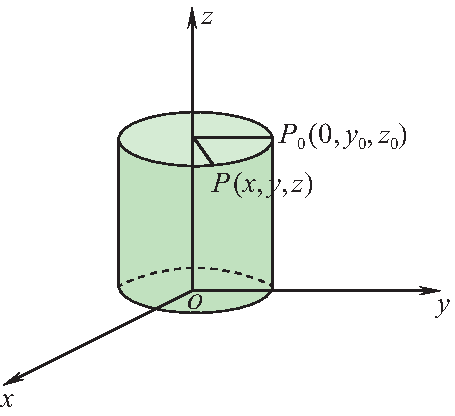
\includegraphics[width = 0.9\linewidth]{pic/C-5/yz}
	\vspace*{-2em}
	\captionof{figure}{旋转曲面}
	\label{旋转曲面}
\end{minipage}

\begin{equation}
	f(y_0,z_0)=0
\end{equation}
\noindent 当曲线$C$绕$z$轴旋转时,$P_0(0,y_0,z_0)$旋转为$P(x,y,z)$,利用旋转前后点到$z$轴的距离不变,我们可以得到$x,y,z$与$y_0,z_0$的对应关系如下:
\begin{equation}
	\begin{cases}
	\,  d=y_0=\pm\sqrt{x^2+y^2}\\
	\, z_0=z\\
	\end{cases}
\end{equation}
又$f(y_0,z_0)=0$,所以旋转后的曲面方程为:
\begin{equation}
	f(\pm\sqrt{x^2+y^2},z)=0
\end{equation}
同理可得,曲线$C$绕$y$轴旋转所得到的曲面方程为
\begin{equation}
	f(y,\pm \sqrt{x^2+z^2})=0
\end{equation}


\subsection{柱面}
\vspace*{-0.5em}
\defination[柱面]

\noindent
\begin{minipage}{0.65\linewidth}
\hspace*{2em}一般地,直线$L$沿定曲线$C$平行移动形成的轨迹叫做\highlight{dy}{\index{ZM@柱面}柱面},定曲线$C$叫做柱面的\highlight{dy}{\index{ZX@准线}准线},动直线$L$叫做柱面的\highlight{dy}{\index{MX@母线}母线},如图 \ref{柱面} 所示。\\
\hspace*{2em} 一般地,只含$x,y$而缺$z$的方程$F(x,y)=0$在空间直角坐标系中表示母线平行于$z$轴的柱面,其准线是$xOy$面上的曲线$C$:$F(x,y)=0$.\\
\hspace*{2em} 类似可知,只含$x,z$而缺$y$的方程$G(x,z)=0$和只含$y,z$而缺$x$的方程$H(y,z)=0$分别表示母线平行于$y$轴和$x$轴的柱面。
\end{minipage}
\begin{minipage}{0.35\linewidth}
	\centering
	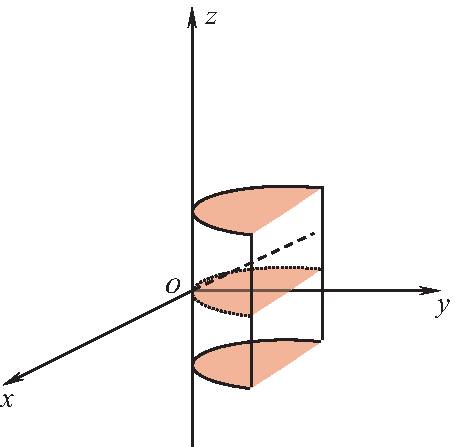
\includegraphics[width = 0.85\linewidth]{pic/C-5/zhuti}
	\vspace*{-1em}
	\captionof{figure}{柱面}
	\label{柱面}
\end{minipage}
	
	\chapter{控制系统的校正}
\thispagestyle{empty}

\section{系统校正设计基础}
\subsection{性能指标}
\begin{enumerate}[1. ]
	\begin{minipage}{0.5\linewidth}
		\item \textbf{时域指标}\vspace*{-0.5em}
		\begin{itemize}
			\item 超调量 \quad $\sigma \%$\vspace*{-0.5em}
			\item 调节时间 \quad $t_{\text{s}}$\vspace*{-0.5em}
			\item 上升时间 \quad $t_{\tau}$\vspace*{-0.5em}
			\item 无差度 \quad $\nu$\vspace*{-0.5em}
			\item 稳态误差、开环增益等
		\end{itemize}
	\item \textbf{复数域指标}\\
	系统的闭环极点在复平面上的分布区域。\vspace*{-0.5em}
	\begin{itemize}
		\item 振荡度 \quad $\varphi$\vspace*{-0.5em}
		\item 衰减度 \quad $\eta$
	\end{itemize}
	\end{minipage}
	\begin{minipage}{0.7\linewidth}
	\item \textbf{频域指标}\vspace*{-0.5em}
	\begin{itemize}
		\item 闭环频率特性
		\begin{itemize}
			\item 峰值比 \quad $\dfrac{M_{\text{m}}}{M_{\text{o}}}$
			\item 峰值频率 \quad $\omega_{\text{m}}$
			\item 频带宽度 \quad $\omega_{\text{b}}$
		\end{itemize}
		
		\item 开环频率特性
		\begin{itemize}
			\item 截止频率 \quad $\omega_{\text{c}}$
			\item 相稳定裕度 \quad $\gamma$
			\item 模稳定裕度 \quad $h$
		\end{itemize}
	\end{itemize}
	\end{minipage}
\end{enumerate}
	
\begin{figure}[!htb]
	\centering
	\includegraphics[width=0.3\linewidth]{pic/复数域性能指标.jpeg}
	\vspace*{-1em}
	\caption{闭环极点的限制区域}
	\label{复数域性能指标}
\end{figure}

\subsection{校正方式}
	在系统基本部分已经确定的情况下,为了保证系统满足动态特性指标,往往需要在系统中附加上一些具有一定动力学性质的附加装置,这些附加装置统称为\dy[校正元件]{JZYJ}或\dy[校正装置]{JZZZ}。
	
	常见的校正装置有以下四种:
	
\begin{equation*}
	\mbox{校正方式}\,
	\begin{cases}
		\, \mbox{串联校正}\\
		\, \mbox{反馈校正}\\
		\, \mbox{(前馈)顺馈校正}\,
		\begin{cases}
			\, \mbox{前置校正}\\
			\, \mbox{干扰补偿}
		\end{cases}
	\end{cases}
\end{equation*}

\begin{figure}[!htb]
	\centering
	\begin{tikzpicture}[circuit ee IEC]
			%定义流程图具体形状
		\node(O) [minimum height=0cm,draw, node distance=1cm,inner sep=5pt] {前置校正};
		\node[bulb] (A)[minimum height=0cm,draw,below of = O,xshift = -2cm,node distance=1.5cm,inner sep=5pt, label = -95:$-$] { };
		\node (B) [minimum height=0cm,draw,below of = O, xshift = -0cm,node distance=1.5cm, inner sep=5pt] {控制器};
		\node[bulb] (D) [minimum height=0cm,draw,below of = O, xshift = 2cm,node distance=1.5cm, inner sep=5pt] { };
		\node (C) [draw, right of = D, node distance = 1.5cm, inner sep = 5pt]{对象};
		\node (E) [draw, left of = A, node distance = 2cm, inner sep = 5pt]{前置校正};

		%连接具体形状
		\draw[arrows={-Stealth}](2cm,1cm) -- (D)  node[midway,right = 0.6cm, above=0.5cm]{干扰$N$};
		\draw[arrows={-Stealth}](2cm,1cm) -- (2cm,0) -- (O) ;
		\draw[arrows={-Stealth}](O) --+(-2cm,0) -- (A) ;
		\draw[arrows={-Stealth}](-7cm,-1.5cm) -- (E)  node[midway,above=0cm]{给定值R};
		\draw[arrows={-Stealth}](E) -- (A) ;
		\draw[arrows={-Stealth}](A) -- (B) ;
		\draw[arrows={-Stealth}](B) -- (D) ;
		\draw[arrows={-Stealth}](D) -- (C) ;
		\draw[arrows={-Stealth}](C) -- +(3cm,0) node[midway,above=0cm]{被控量C} ;
		\draw[arrows={-Stealth}](5.2cm,-1.5cm) --+(0,-1.5cm) --+(-7.2cm, -1.5cm) -- (A) ;
	\end{tikzpicture}
	\caption{前置校正}
	\label{前置校正}
\end{figure}
\begin{figure}[!htb]
	\centering
	\begin{tikzpicture}[circuit ee IEC]
		%定义流程图具体形状
		\node[bulb] (A) [inner sep = 5pt, draw, label = -95:$-$]{};
		\node (B) [inner sep = 5pt, right of = A, node distance = 2cm, draw]{串联校正};
		\node[bulb] (C) [inner sep = 5pt, right of = B, node distance = 2cm, draw, label = -95:$-$]{};
		\node (D) [inner sep = 5pt, right of = C, node distance = 2cm, draw]{控制器};
		\node (E) [inner sep = 5pt, right of = D, node distance = 2cm, draw]{对象};
		\node (F) [inner sep = 5pt, below of = E, xshift = -12mm, node distance = 1.2cm, draw]{反馈校正};
		
		%连接具体形状
		\draw[arrows={-Stealth}](-3cm, 0cm) -- (A)  node[midway,above=0cm]{给定值R};
		
		\draw[arrows={-Stealth}](A) -- (B) ;
		\draw[arrows={-Stealth}](B) -- (C) ;
		\draw[arrows={-Stealth}](C) -- (D) ;
		\draw[arrows={-Stealth}](D) -- (E) ;
		\draw[arrows={-Stealth}](E) -- +(3cm,0) node[midway,above=0cm]{被控量C} ;
		\draw[arrows={-Stealth}](9.5cm, 0cm) -- +(0cm, -1.2cm) -- (F) ;
		\draw[arrows={-Stealth}](F) -- (4cm, -1.2cm) -- (C) ;
		\draw[arrows={-Stealth}](9.5cm, -1.2cm) -- +(0cm, -1.2cm) -- (0cm,-2.4cm) -- (A) ;
	\end{tikzpicture}
	\caption{串联校正和反馈校正}
	\label{串联校正和反馈校正}
\end{figure}

\section{串联校正}
加入串联校正后的系统结构图如图\ref{系统的串联校正}所示。其中$G_{\text{c}}(s)$表示了串联校正装置的传递函数,$G(s)$表示系统不变部分的传递函数。
\begin{equation*}
	\mbox{串联校正} \,
	\begin{cases}
		\, \mbox{超前校正}\\
		\, \mbox{滞后校正}\\
		\, \mbox{滞后—超前校正}
	\end{cases}
\end{equation*}
\begin{figure}[!htb]
	\centering
	\begin{tikzpicture}[circuit ee IEC]
		%定义流程图具体形状
		\node[bulb] (A) [inner sep = 5pt, draw, label = -95:$-$]{};
		\node (B) [inner sep = 5pt, right of = A, node distance = 2cm, draw]{$G_{\text{c}}(s)$};
		\node (C) [inner sep = 5pt, right of = B, node distance = 2cm, draw]{$G(s)$};
		
		%连接具体形状
		\draw[arrows={-Stealth}](-1.5cm, 0cm) -- (A);
		
		\draw[arrows={-Stealth}](A) -- (B) ;
		\draw[arrows={-Stealth}](B) -- (C) ;
		\draw[arrows={-Stealth}](C) -- +(2cm,0) ;
		\draw[arrows={-Stealth}](5.2cm , 0cm) -- (5.2cm, -1.2cm) -- (0cm,-1.2cm) -- (A) ;
	\end{tikzpicture}
	\vspace*{-0.5em}
	\caption{系统的串联校正}
	\label{系统的串联校正}
\end{figure}
\vspace*{-1.5em}

\subsection{相位超前校正}\vspace*{-0.5em}\index{CQJZ@超前校正}
\begin{enumerate}[1. ]
	\item \textbf{相位超前校正的特点}\vspace*{-0.5em}
	\begin{itemize}
		\item 超前补偿可显著改善系统的动态品质而对系统稳态性能影响较小;
		\item 但经超前补偿后的系统高频噪声的抑制能力会下降。
	\end{itemize}

	\item \textbf{超前补偿器的数学模型}
	\begin{align}
		G_{\text{c}}(s) &= K_c \dfrac{aTs + 1}{Ts + 1},\quad \quad a>1\\
		\varPhi(\omega) = \angle G_{\text{c}}(\j \omega) &= \arctan aT\omega - \arctan T\omega
	\end{align}

\begin{figure}[!htb]
	\centering
	\includegraphics[width=0.55\linewidth]{pic/超前bode.pdf}
	\vspace*{-1em}
	\caption{超前校正的Bode图}
	\label{超前Bode}
\end{figure}
其中,
\begin{align}
	\omega_\text{m} &= \dfrac{1}{T \sqrt{a}}\\
	\varphi_\text{m} &= \arcsin \dfrac{a - 1}{a + 1}
\end{align}

	\item \textbf{超前补偿器的设计步骤}\\
	设系统原传递函数为$G_1(s)$,补偿器的传递函数为$G_\text{c}(s)$.\vspace*{-0.5em}
	\begin{enumerate}[\textbf{步骤} 1 ]
		\item \textbf{确定需要增加的相角}$\varphi_{\text{m}}$
		\begin{equation}
			\varphi_{\text{m}} = \gamma' - \gamma +(5\degree \sim 12 \degree)
		\end{equation}
		其中,$\gamma'$指的是期望的相稳定裕度。
		
		\item \textbf{确定参数$a$}
		\begin{align}
			a = \dfrac{1 + \sin \varphi_\text{m}}{1 - \sin \varphi_\text{m}}
		\end{align}
		
		\item \textbf{确定新的截止频率$\omega_{\text{c}}'$}
		\begin{equation}
			20 \lg A(\omega_{\text{c}}') = - 10 \lg a
		\end{equation}
		
		\item \textbf{确定新的转折频率对应的$T$}
		\begin{align}
			\omega_{\text{c}}' = \omega_{\text{m}} = \dfrac{1}{T \sqrt{a}} \quad \Rightarrow \quad T = \dfrac{1}{\omega_{\text{c}}'\sqrt{a}}
		\end{align}
	\end{enumerate}
若已知$\omega_{\text{c}}' \ge \omega^*$,则步骤可以简化为
\begin{enumerate}[\textbf{步骤}]
	\item $2^*\,\,$ \textbf{确定新的截止频率$\omega_{\text{c}}'$}
	\begin{equation}
		\omega_{\text{c}}' = \omega^* + (3 \sim 5)
	\end{equation}
	
	\item $3^*\,\,$ \textbf{确定补偿器的参数和转折频率}
	\begin{equation}
		10 \lg a = - 20 \lg|G(\j \omega_{\text{c}}')| \quad \Rightarrow \quad a \quad \Rightarrow \quad \dfrac{1}{T} = \sqrt{a}\omega_{\text{c}}
	\end{equation}
\end{enumerate}
\end{enumerate}
\clearpage

\vspace*{-3em}
\examples \label{6.1}考虑如下系统,其开环传递函数用$G(s)$表示
\begin{figure}[!htb]
	\centering
	\begin{tikzpicture}[circuit ee IEC,node distance=1.2cm]
		\node[bulb] (A)  [draw, inner sep=5pt,label=-80:$-$] {};
		\node (B) [draw, inner sep =4pt,right of = A, node distance = 2cm]{$\,\dfrac{K}{s(0.1s + 1)}\,$};
		
		\draw[arrows={-Stealth}] (-1cm,0cm) -- (A)node[near start, above = 0cm]{$R(s)$};
		\draw [arrows={-Stealth}] (A) -- (B);
		\draw[arrows={-Stealth}] (B) -- (4cm,0cm)node[near end, above =0cm]{$C(s)$};
		\draw[arrows={-Stealth}] (3.5cm,0cm) -- +(0cm, -1cm) -- (0cm,-1cm) -- (A);
	\end{tikzpicture}
	\caption{\ref{6.1} 系统结构图}
	\label{F6.1.1}
\end{figure}

要求设计一个串联补偿器,使得静态速度误差$e_{\text{ss}} \le 0.01, \gamma \ge 45\degree, \omega_{\text{c}} \ge 40$rad/s.

\solve 根据上面的步骤解题。
\begin{enumerate}[\textbf{第} 1 \textbf{步} ]
	\item \textbf{确定满足稳态误差的开环增益$K$}\\
	由于这是一个\RMN[1]型系统,所以$e_{\text{ss}} = \dfrac{1}{K} \le 0.01 \quad \Rightarrow \quad K \ge 100$.不妨取$K = 100.$
	
	\item \textbf{求此时的相稳定裕度}\\
	经过计算,绘制Bode图如图\ref{F6.1.2}.
	\begin{figure}[!htb]
		\centering
		\includegraphics[width=0.45\linewidth]{pic/6.1.pdf}
		\vspace*{-1em}
		\caption{\ref{6.1}修正前的Bode图}
		\label{F6.1.2}
	\end{figure}

	从而得到
	\begin{align*}
		\omega_{\text{c}} &= 31 \text{rad/s}\\
		\gamma &= 17.9 \degree
	\end{align*}
	
	\item \textbf{确定新的截止频率}\\
	由于要求$\omega_{\text{c}} \ge 40$rad/s,不妨选取
	\[
	\omega_{\text{c}}' = \omega_{\text{m}} = 44 \text{rad/s}
	\]
	
	\item \textbf{计算未经校正系统的幅值}
	\[
	20 \lg |G(\j \omega_{\text{c}}')| = -6 \text{dB} 
	\]
	
	\item \textbf{确定补偿器的参数和转折频率}
	\[
	10 \lg a = 6 \text{dB} \quad \Rightarrow \quad a = 4 \quad \Rightarrow \quad \dfrac{1}{T} = \sqrt{a}\omega_{\text{c}} = 88
	\]
\end{enumerate}
所以
\[
\dfrac{G_\text{c}(s)}{K_\text{c}} = \dfrac{aTs + 1}{Ts + 1} = \dfrac{0.04544s + 1}{0.01136s + 1}
\]
用Matlab绘制补偿前后系统的Bode图如图\ref{F6.1.3}.
\begin{figure}[!htb]
	\centering
	\includegraphics[width=0.6\linewidth]{pic/6.1.2.pdf}
	\vspace*{-1em}
	\caption{\ref{6.1}修正前后的Bode图}
	\label{F6.1.3}
\end{figure}

\subsection{相位滞后校正}\vspace*{-0.5em}\index{ZHJZ@滞后校正}
\begin{enumerate}[1. ]
	\item \textbf{相位滞后校正的特点}\\
	(1) 滞后校正的主要功能是抑制高频干扰并使经校正后的系统具有较大的相稳定裕度。\\
	(2) 滞后补偿器本质上是一个低通滤波器,因此,滞后 校正可允许低频段有高增益。\\
	(3) 离虚轴很近的极点会对系统的过渡过程产生影响, 使响应变慢(尽管其附近的零点可使幅值变小)。\\
	(4) 截止频率$\omega_{\text{c}}' < \omega_{\text{c}}$,从而使调节时间$t_\text{s}$增加。
	
	\item \textbf{滞后补偿器的数学模型}
	\begin{align}
		G_{\text{c}}(s) &= K_c \dfrac{bTs + 1}{Ts + 1}, \quad \quad 0 < b < 1\\
		\varPhi(\omega) = \angle G_{\text{c}}(\j \omega) &= \arctan bT\omega - \arctan T\omega
	\end{align}
	
	\begin{figure}[!htb]
		\centering
		\includegraphics[width=0.55\linewidth]{pic/滞后bode.pdf}
		\vspace*{-1em}
		\caption{滞后校正的Bode图}
		\label{滞后Bode}
	\end{figure}
	其中,
	\begin{align}
		\omega_\text{m} &= \dfrac{1}{T \sqrt{b}}\\
		\varphi_\text{m} &= \arcsin \dfrac{1 - b}{1 + b}
	\end{align}
	
	\item \textbf{滞后补偿器的设计步骤}\\
	设系统原传递函数为$G_1(s)$,补偿器的传递函数为$G_\text{c}(s)$.\vspace*{-0.5em}
	\begin{enumerate}[\textbf{步骤} 1 ]
		\item \textbf{根据给定的$\gamma^*$确定$\omega_{\text{c}}'$}
		\begin{equation}
			\gamma' = \gamma^* + (5\degree \sim 12 \degree)
		\end{equation}
		然后根据渐近幅频特性曲线和Bode图计算$\omega_{\text{c}}'$。
		
		\item \textbf{确定参数$b$}
		\begin{align}
			20 \lg b = -20 \lg |G_1(\j \omega_{\text{c}}')| \quad \Rightarrow \quad b = \dfrac{1}{G_1(\j \omega_{\text{c}}')}
		\end{align}
		
		\item \textbf{确定新的转折频率$\dfrac{1}{bT},\dfrac{1}{T}$}
		\begin{align}
			\dfrac{1}{bT} = (0.1 \sim 0.5)\omega_{\text{c}}'
		\end{align}
	\end{enumerate}
\end{enumerate}

\examples \label{6.2}已知单位负反馈系统的开环传递函数为
\[
G(s) = \dfrac{1}{s(0.5s + 1)}
\]
要求在单位斜坡输入下的稳态误差为0.05且相稳定裕度至少45$\degree$,设计串联校正补偿器。

\solve 根据上面的步骤解题。
\begin{enumerate}[\textbf{第} 1 \textbf{步} ]
	\item \textbf{确定满足稳态误差的开环增益$K$}\\
	$G_1(s) = K \dfrac{1}{s(0.5s + 1)}$,由于这是一个\RMN[1]型系统,所以$e_{\text{ss}} = \dfrac{1}{K} = 0.05 \quad \Rightarrow \quad K = 20$.
	
	\item \textbf{求此时的相稳定裕度}\\
	经过计算,绘制Bode图如图\ref{F6.2.1}.
	\begin{figure}[!htb]
		\centering
		\includegraphics[width=0.7\linewidth]{pic/6.2.1.pdf}
		\vspace*{-1em}
		\caption{\ref{6.2}修正前的Bode图}
		\label{F6.2.1}
	\end{figure}
	
	可以用渐近幅频特性曲线计算截止频率和对应的相温度裕度
	\begin{align*}
		L(\omega) = 20\lg K - 20\lg \omega - 20 \lg T_1\omega = 20\lg 20 - 20\lg \omega &- 20 \lg 0.5\omega = 0 \quad \Rightarrow \quad \omega_{\text{c}} = 2\sqrt{10} \approx 6.3 \,\,\text{rad/s}\\
		\varphi(\omega_{\text{c}}) = -90\degree - \arctan(0.5 \omega_{\text{c}}) &= -162\degree \quad \Rightarrow \quad \gamma = 18\degree
	\end{align*}
	
	\item \textbf{确定新的截止频率}\\
	取$\gamma' = 50 \degree$($5\degree$用于补偿相位滞后),得
	\[
	\varphi(\omega_{\text{c}}) = -130 \degree \quad \Rightarrow \quad \omega_{\text{c}}' = 1.5 \,\,\text{rad/s}
	\]
	
	\item \textbf{计算未经校正系统的幅值}
	\[
	20 \lg |G(\j \omega_{\text{c}}')| = 20 \text{dB} 
	\]
	
	\item \textbf{确定补偿器的参数和转折频率}
	\[
	20 \lg b = -20 \text{dB} \quad \Rightarrow \quad b = 0.1 
	\]
	选择
	\[
	\dfrac{1}{bT} = 0.1 \omega_{\text{c}}' = 0.15 \quad \Rightarrow \quad \dfrac{1}{T} = 0.015
	\]
	
\end{enumerate}
\begin{figure}[!htb]
	\centering
	\includegraphics[width=0.6\linewidth]{pic/6.2.2.pdf}
	\vspace*{-1em}
	\caption{\ref{6.2}确定新的截止频率}
	\label{F6.2.2}
\end{figure}
所以设计的补偿器为
\[
\dfrac{G_\text{c}(s)}{K_\text{c}} =  \dfrac{bTs + 1}{Ts + 1} = \dfrac{6.67s + 1}{66.7s + 1}
\]
用Matlab绘制补偿前后系统的Bode图如图\ref{F6.2.3}.
\begin{figure}[!htb]
	\centering
	\includegraphics[width=0.6\linewidth]{pic/6.2.3.pdf}
	\vspace*{-1em}
	\caption{\ref{6.2}修正前后的Bode图}
	\label{F6.2.3}
\end{figure}

\subsection{超前—滞后校正}\vspace*{-0.5em}\index{CQZHJZ@超前—滞后校正}
\begin{enumerate}[1. ]
	\item \textbf{相位滞后校正的特点}\\
	(1) 超前校正可改善响应速度和相稳定裕度,但会导致频宽增加,不利于高频干扰的抑制。\\
	(2) 滞后校正可改善相稳定裕度,但有会使调节时间变长。\\
	(3) 因此,希望用滞后—超前校正将以上两种校正器的优点结合在一起。
	
	\item \textbf{滞后补偿器的数学模型}
	\begin{align}
		G_{\text{c}}(s) &= K_c\left(\dfrac{bT_1s + 1}{T_1s + 1}\right) \left(\dfrac{aT_2s + 1}{T_2s + 1}\right), \quad \quad a>1, \, 0 < b < 1, \, bT_1 > aT_2\\
		\varPhi(\omega) &= \angle G_{\text{c}}(\j \omega) = \arctan bT\omega - \arctan T\omega
	\end{align}
	通常要求滞后部分的两个转折频率要低于超前部分的两个转折频率。
	
	\begin{figure}[!htb]
		\centering
		\includegraphics[width=0.55\linewidth]{pic/超前滞后Bode图.pdf}
		\vspace*{-1em}
		\caption{超前—滞后校正的Bode图}
		\label{超前滞后Bode}
	\end{figure}
\end{enumerate}

\vspace*{-2.5em}

\warn[
\textbf{\large 频率校正总结}\\
\hspace*{1em} 三种校正方法均基于镜像原理,一般地:
\vspace*{-0.5em}
{
	\begin{enumerate}[\hspace*{2em} 1. ]
		\item 根据相稳定裕度确定校正后的截止频率$\omega_{\text{c}}'$
		\vspace*{-0.5em}
		
		\item 利用镜像原理求校正器的交接频率,即新的截止频率$\omega_{\text{c}}'$处补偿器的幅值和被补偿系统的幅值互补,相加为0.
	\end{enumerate}
}
]

\subsection{PID校正器}
\begin{enumerate}
	\item \textbf{PD校正器}\\
	\dy[PD校正器]{PDJZQ}又称为\dy[比例—微分校正]{BLWFJZ},其传递函数
	\begin{align}
		G_{\text{c}}(s) & = K_{\text{d}} s + K_{\text{p}}\\
		& = K_{\text{p}}\left(\dfrac{K_{\text{d}}}{K_{\text{p}}}s + 1\right) = K_{\text{p}}(Ts + 1)
	\end{align}
	其作用相当于超前校正。
	
	\item \textbf{PI校正器}\\
	\dy[PI校正器]{PIJZQ}又称为\dy[比例—积分校正]{BLJFJZ},其传递函数
	\begin{align}
		G_{\text{c}}(s) = K_{\text{p}}  + \dfrac{1}{T_{\text{i}} s} = \dfrac{1}{T_{\text{i}}} \dfrac{T_{\text{i}} K_{\text{p}}s + 1}{s}
	\end{align}
	其作用相当于滞后校正。
	
	\item \textbf{PID校正器}\\
	\dy[PID校正器]{PIDJZQ}又称为\dy[比例—积分—微分校正]{BLJFWFJZ},其传递函数
	\begin{align}
		G_{\text{c}}(s) = K_{\text{p}}  + K_\text{d} s +  \dfrac{1}{T_{\text{i}} s} = \dfrac{T_\text{i} K_{\text{d}}s^2 + T_\text{i} K_\text{p}s + 1}{T_{\text{i}}s}
	\end{align}
	其作用相当于超前—滞后校正。

\end{enumerate}


\section{串联校正的根轨迹方法}
\subsection{增加零、极点对系统性能的影响}
\noindent \textbf{1. 增加极点对系统性能的影响}


在开环传递函数中增加一个极点会使根轨迹向虚轴偏移,降低相对稳定性及延长调节时间。


\noindent \textbf{2. 增加零点对系统性能的影响}


在开环传递函数中增加一个零点会使根轨迹向左偏移,使系统更加稳定且响应速度更快。

\subsection{根轨迹校正器设计}

\noindent \textbf{1. 数学模型}
\begin{equation}
	G_{\text{c}}(s) = K_\text{c} \dfrac{aTs+1}{Ts + 1} = K_\text{c}^* \dfrac{s + \dfrac{1}{aT}}{s + \dfrac{1}{T}} = K_\text{c}^* \dfrac{s - z}{s - p}, \quad a>1
\end{equation}

\noindent \textbf{2. 设计步骤}
\begin{enumerate}[\hspace*{2em} \textbf{步骤} 1 ]
	\item \textbf{由二阶系统的性能指标确定主导极点}
	\begin{equation}
		s_{1,2} = \zeta \omega_{\n} \pm \j \sqrt{1 - \zeta^2} \omega_{\n}
	\end{equation}
	\item \textbf{绘原系统的闭环根轨迹,确定是否仅调节系统的开环增益$\bm{K^*}$就可以达到期望的闭环极点}
	\item \textbf{确定校正器的类型}
	\item \textbf{确定补偿器零点和极点的位置}\\
	通常有无数种取法,工程上一般这么做\vspace*{-0.5em}
	\begin{enumerate}[\hspace*{1em}1.]
		\item 确定满足$\pm180\degree(2k+1)$条件时,需要增加的相角$\varphi$
		\item 利用角平分线补偿相角以确定补偿器零点和极点的位置,如图\ref{根轨迹超前}.
		\begin{enumerate}[(1)  ]
			\item 作水平线$PA$及直线$PO$
			\item 作$\angle APO$的角平分线$PB$
			\item 过$P$点作两条直线$PC,PD$ ,使得与$PB$的角度为$\dfrac{\varphi}{2}$.$PC$和$PD$与横轴的交点就是补偿器极点和零点的位置
			\item 利用角度关系解三角形确定零点$z$和极点$p$的值
		\end{enumerate}
	\end{enumerate}
	\begin{figure}[!htb]
		\centering
		\includegraphics[width=0.55\linewidth]{pic/根轨迹超前.pdf}
		\vspace*{-1em}
		\caption{利用角平分线补偿相角以确定补偿器零点和极点示意图}
		\label{根轨迹超前}
	\end{figure}
	\item \textbf{确定补偿器开环增益$\bm{K_\text{c}^*}$的值}\\
	利用在主导极点处的模方程$\big|G'(s_1)\big|=\Big|G'\left(\zeta \omega_{\n} + \j \sqrt{1 - \zeta^2} \omega_{\n}\right)\Big| = 1$确定开环增益$K_\text{c}^*$的值。
\end{enumerate}

\examples \label{6.4}已知单位负反馈系统的开环传递函数为
\begin{equation}
	G(s) = \dfrac{4}{s(s+2)}
\end{equation}
设计校正装置,使得$t_\text{s} = 1.75 \, \text{s},\,\, \sigma \% = 16.3\%.$

\solve 由上述方法解题
\begin{enumerate}[\textbf{第} 1 \textbf{步}]
	\item \textbf{由性能指标确定主导极点}\\
	由
	\[
	\sigma \% = \e^{-\frac{\pi \zeta}{\sqrt{1 - \zeta^2}}} \times 100\% = 16.3\%, \, t_\text{s} = \dfrac{3.5}{\zeta \omega_{\n}} = 1.75 \quad \Rightarrow \quad \zeta = 0.5\,(\beta = 60 \degree),\,\, \omega_{\n} = 4 \,\text{rad/s}
	\]
	得到期望的闭环主导极点为
	\[
	s_{1,2} = \zeta \omega_{\n} \pm \j\sqrt{1 - \zeta^2}\omega_{\n} = -2 \pm  \j2\sqrt{3}
	\]
	
	\item \textbf{绘制校正前系统的闭环根轨迹}
	\begin{figure}[!htb]
		\centering
		\includegraphics[width=0.25\linewidth]{pic/6.4.1.pdf}
		\caption{\ref{6.4}$\,$校正前系统根轨迹图}
	\end{figure}
	
	\item \textbf{确定校正器的类型}\\
	由根轨迹图可以看出,期望的主导极点在校正前系统的远离虚轴侧,因此,适合采用超前校正器来改变系统的主导极点。设补偿器为
	\[
	G_\text{c}(s) = K_\text{c}\dfrac{s - z}{s -p}, z>p
	\]
	校正后的系统可以表示为
	\[
	G'(s) = G(s)G_\text{c}(s) = \dfrac{4}{s(s+2)}\cdot K_\text{c}\dfrac{s-z}{s-p}
	\]
	
	\item \textbf{确定补偿器零点和极点的位置}
	\begin{enumerate}[1.]
		\item 确定补偿器的相角$\varphi$,校正后的系统在主导极点$s_1 = -2 + \j 2 \sqrt{3}$处满足相角方程
		\[
		\angle G'(s) = \angle G(s) + \angle G_\text{c}(s) = \angle \dfrac{4}{s(s+2)}\Bigg|_{s = 2 + \j 2 \sqrt{3}} + \varphi = 180\degree(2k + 1)
		\]
		计算得到
		\[
			\varphi = 180\degree -  \angle \dfrac{4}{s(s+2)}\Bigg|_{s = 2 + \j 2 \sqrt{3}} = 180 \degree - 150\degree = 30 \degree
		\]
		
		\item 利用角平分线等分法确定零点和极点的位置
		\begin{figure}[!htb]
			\centering
			\includegraphics[width=0.55\linewidth]{pic/根轨迹超前.pdf}
			\vspace*{-1em}
			\caption{\ref{6.4}$\,$确定补偿器零点和极点图}
			\label{F6.4}
		\end{figure}
	
		由正弦定理,
		\[
		 |OD| = \dfrac{|OP|}{\sin \left(90 \degree + \dfrac{\varphi}{2} - \dfrac{\beta}{2} \right)} \cdot \sin \left(90 \degree - \dfrac{\varphi}{2} - \dfrac{\beta}{2}\right) = \dfrac{|-2+\j 2 \sqrt{3}|}{\sin (90\degree + 15\degree - 30\degree)}\cdot \sin (90\degree - 15\degree - 30 \degree)=2.93
		\]
		所以,$z = -2.93$,同理可以得到$p = -5.46.$所以校正器和校正后的系统方程分别为
		\begin{align*}
			G_\text{c} (s) &=K_\text{c}^* \dfrac{s + 2.93}{s + 5.46}\\[0.5em]
			G'(s) &= K_\text{c}^* \dfrac{4(s + 2.93)}{s(s+2)(s+5.46)} = K^*\dfrac{s + 2.93}{s(s+2)(s+5.46)} \quad (K^* = 4K_\text{c}^*)
		\end{align*}
	
	\end{enumerate}
	
		\item \textbf{确定补偿器开环增益$\bm{K_\text{c}^*}$的值}\\
		由模方程,得
		\[
			\left|K^* \dfrac{4(s + 2.93)}{s(s+2)(s+5.46)}\right|_{s = -2 + \j 2\sqrt{3}} = 1 \quad \Rightarrow \quad K^* = 18.7 \quad \Rightarrow \quad K_\text{c}^* = K^*/4 = 4.68
		\]
\end{enumerate}
所以校正器和校正后的系统方程分别为
\begin{align*}
	G_\text{c} (s) &=4.68 \dfrac{s + 2.93}{s + 5.46}\\[0.5em]
	G'(s) &= 18.7 \dfrac{4(s + 2.93)}{s(s+2)(s+5.46)}
\end{align*}

\subsection{根轨迹的滞后校正}
若系统具有满意的动态性能但稳态性能不佳,则可考虑采用滞后校正器。即系统有两个主导极点且具有满意的动态响应,但静态速度误差不满足要求。\\[0.5em]
\textbf{根轨迹滞后校正的基本要求}
\begin{itemize}
	\item 不显著改变原闭环主导极点的位置
	\item 开环增益需要调高到满足稳态误差
\end{itemize}

\noindent \textbf{1. 数学模型}
\begin{equation}
	G_{\text{c}}(s) = K_\text{c} \dfrac{bTs+1}{Ts + 1} = K_\text{c}^* \dfrac{s + \dfrac{1}{bT}}{s + \dfrac{1}{T}} = K_\text{c}^* \dfrac{s - z}{s - p}, \quad 0<b<1
\end{equation}

\noindent \textbf{2. 设计步骤}
\begin{enumerate}[\hspace*{2em} \textbf{步骤} 1 ]
	\item \textbf{绘制原系统的根轨迹,并根据动态性能指标确定期望的闭环主导极点在复平面上的位置}
	\item \textbf{确定校正器的类型}
	\item \textbf{求满足指标的稳态误差系数并确定补偿器需要增加的开环增益}
	\item \textbf{利用加角线法确定零点和极点的位置}\\
	过$s_1$作一条直线,与原点$O$和$s_1$间的夹角为$6\degree \sim 10\degree$ 且与横轴交于$E$点,如图\ref{根轨迹滞后}.
	\begin{figure}[!htb]
		\centering
		\includegraphics[width=0.7\linewidth]{pic/根轨迹滞后.pdf}
		\vspace*{-1em}
		\caption{利用加角线法确定零点和极点的位置}
		\label{根轨迹滞后}
	\end{figure}

	进而,在$E$点的右侧选择零点和极点.
	\item \textbf{计算校正后系统的期望主导极点并确定补偿器开环增益$\bm{K_\text{c}^*}$的值}\\
	由于动态性能指标不变,利用给定的阻尼比$\zeta$并利用待定系数法确定主导极点及$K_\text{c}^*$的值。
\end{enumerate}

\examples \label{6.5} 已知单位负反馈系统的开环传递函数为
\[
G(s) = \dfrac{1.06}{s(s+1)(s+2)}
\]
设计一个校正器,使得其阻尼比为$\zeta = 0.5$,静态速度误差$e_{\text{ss}} = 0.2.$

\solve 由上述方法解题
\begin{enumerate}[\textbf{第} 1 \textbf{步}]
	\item \textbf{绘制原系统的根轨迹,并根据动态性能指标确定期望的闭环主导极点在复平面上的位置}\\
	由系统的闭环特征方程
	\[
	s(s+1)(s+2)+1.06 = 0
	\]
	可以解得系统的主导极点为
	\[
	s_{1,2} = -0.33 \pm \j 0.59
	\]
	\item \textbf{确定校正器的类型}\\
	其中,$s_{1,2}$与$60 \degree$线接近,而$K_\text{v} = \dfrac{1.06}{2} = 0.53 \le 5$,所以动态性能很好但是不满足静态误差,需要滞后校正器。设滞后校正器为
	\[
	G_{\text{c}}(s) = K_\text{c}^* \dfrac{s - z}{s - p}
	\]
	\item \textbf{求满足指标的稳态误差系数并确定补偿器需要增加的开环增益}\\
	\[
	K_\text{v}^* = \dfrac{1}{e_{\text{ss}}} = \dfrac{1}{0.2} = 5, \quad \Rightarrow \quad K^* = \dfrac{K_\text{v}^*}{K_\text{v}} \approx 10.
	\]
	\item \textbf{利用加角线法确定零点和极点的位置}\\
	过$s_1$作一条直线,与原点$O$和$s_1$间的夹角为$6\degree \sim 10\degree$ 且与横轴交于$E$点,如图\ref{6.5.2}.
	\begin{figure}[!htb]
		\centering
		\includegraphics[width=0.7\linewidth]{pic/根轨迹滞后.pdf}
		\vspace*{-1em}
		\caption{\ref{6.5}$\,$确定零点和极点的位置}
		\label{6.5.2}
	\end{figure}

	进而,在$E$点的右侧选择零点和极点:
	\[
	z = -0.05, \quad p = -0.005
	\]
	则校正后的系统为
	\[
	G'(s) = K_c^* \dfrac{s + 0.05}{s + 0.005} \dfrac{1.06}{s(s+1)(s+2)} = K^* \dfrac{s + 0.05}{s(s+1)(s+2)(s+0.005)}
	\]
	\item \textbf{计算校正后系统的期望主导极点并确定补偿器开环增益$\bm{K_\text{c}^*}$的值}\\
	闭环特征方程为
	\begin{align*}
		& \quad \, s(s+1)(s+2)(s+0.005) + K^*s(s+0.05) \\&= s^4 + \dfrac{601}{200}s^3 + \dfrac{403}{200}s^2 + \dfrac{200K^*+2}{200}s + \dfrac{10}{200}K^*\\
		& = (s^2 +2\zeta \omega_\n s + \omega_{\n}^2)(s + s_3)(s + s_4)
	\end{align*}
	
	
	
	
\end{enumerate}
所以校正器和校正后的系统方程分别为
\begin{align*}
	G_\text{c} (s) &=4.68 \dfrac{s + 2.93}{s + 5.46}\\[0.5em]
	G'(s) &= 18.7 \dfrac{4(s + 2.93)}{s(s+2)(s+5.46)}
\end{align*}




\section{反馈校正}
\begin{figure}[!htb]
	\centering
	\begin{tikzpicture}[circuit ee IEC,node distance=1.2cm]
		\node[bulb] (A) [draw, inner sep = 5pt, label=-85:$-$]{};
		\node (A1) [draw, inner sep = 6pt, right of  = A, node distance = 1.5cm]{$G_1(s)$};
		\node[bulb] (B) [draw, right of = A1, node distance = 1.5cm,inner sep = 5pt, label=-85:$-$]{};
		\node (C) [draw, inner sep =6pt, right of = B,node distance =1.5cm]{$G_2(s)$};
		\node (C1) [draw, inner sep =6pt, below of = C,node distance =1.5cm]{$H(s)$};
		\node (D) [draw, inner sep =6pt, right of = C,node distance = 2.5cm]{$G_3(s)$};
		
		\draw[arrows={-Stealth}] (-1.2cm, 0cm) -- (A)node[near start, above = 0cm]{$R(s)$};
		\draw[arrows={-Stealth}] (A) -- (A1);
		\draw[arrows={-Stealth}] (A1) -- (B);
		\draw[arrows={-Stealth}] (B) -- (C);
		\draw[arrows={-Stealth}] (C) -- (D);
		\draw[arrows={-Stealth}] (D) -- +(2cm, 0cm)node[near end, above = 0cm]{$C(s)$};
		\draw [arrows={-Stealth}] (5.7cm, 0cm) -- +(0cm, -1.5cm) -- (C1);
		\draw [arrows={-Stealth}] (C1) -- +(-1.5cm, 0cm) -- (B);
		\draw [arrows={-Stealth}] (8.3cm, 0cm) -- +(0cm, -2.3cm) -- (0cm, -2.3cm) -- (A);
		
	\end{tikzpicture}
	\caption{反馈校正系统结构图}
	\label{反馈校正系统结构图}
\end{figure}

引进$H(s)$的作用是希望$\varPhi_2(s)$的特性使整个闭环系统的品质得到改善。

\subsection{利用反馈改变局部结构、参数}
如图\ref{反馈校正系统结构图}.通过反馈校正可以改变局部结构和参数。
\vspace*{1em}

\noindent \textbf{1. 用位置反馈包围积分环节}
\begin{align}
	G_2(s) = \dfrac{K}{s}
\end{align}
引入反馈
\begin{align}
	H(s) = K_f
\end{align}
得到
\begin{equation}
	\varPhi_2(s) = \dfrac{1}{K_f} \cdot \dfrac{1}{Ts + 1}, \quad T = \dfrac{1}{KK_f}
\end{equation}
所以反馈校正后的结果为
\begin{itemize}
	\item 积分环节变成一阶系统,使系统的无差度下降
	\item 若$T \downarrow$,相位滞后减少,可提高系统的稳定性
\end{itemize}
\vspace*{1.5em}


\noindent \textbf{2.用速度反馈包围惯性、积分和放大环节}
\begin{align}
	G_2(s) = \dfrac{K}{s(Ts + 1)}
\end{align}
引入速度反馈
\begin{align}
	H(s) = K_t s
\end{align}
得到
\begin{align}
	\varPhi_2(s) = \dfrac{K_1}{(Ts + 1)}
\end{align}
所以反馈校正后的结果为
\begin{itemize}
	\item 没有改变典型环节的类型,保持了积分环节,系统的无差度无改变
	\item 因$K_t>0 \rightarrow T_1<T$,可增大系统频宽,有利于加快系统响应
\end{itemize}
\vspace*{1.5em}

\noindent \textbf{3. 用速度反馈包围一个小阻尼的二阶振荡环节和放大环节}
\begin{align}
	G(s) = \dfrac{K \omega_\n^2}{s^2 + 2\zeta \omega_\n s + \omega_{\n}^2 }, \quad 0< \zeta < 1
\end{align}
引入速度反馈
\begin{align}
	H(s) = K_t s
\end{align}
得到
\begin{align}
	\varPhi_2(s) = \dfrac{K\omega_\n^2}{s^2 + 2 \left(\zeta + 0.5 KK_t \omega_\n \right) \omega_\n s+ \omega_\n^2}
\end{align}
所以反馈校正后的结果为:加入速度反馈,增加了阻尼,减弱了小阻尼环节的不利影响。

\noindent \textbf{4. 速度反馈信号再经过一个微分网络}
\begin{align}
	G_2(s) = \dfrac{K_1}{(T_1 s + 1)}
\end{align}
速度反馈信号再经过一个微分网络
\begin{align}
	H(s) = K_t s \dfrac{T_2 s}{T_2 s + 1} = \dfrac{K_t T_2 s^2}{T_2s + 1}
\end{align}
\begin{align}
	\varPhi_2(s) &= \dfrac{K_1(T_2 s + 1)}{s \left[T_1T_2s^2 + \left(T_1 + T_2 + T_2K_1K_t\right)s + 1 \right]}\notag \\[0.5em]
	& =\dfrac{K_1(T_2s + 1)}{s(T's + 1)(T''s + 1)} =\dfrac{K_1(T_1s + 1)(T_2s + 1)}{s(T_1s + 1)(T's + 1)(T''s + 1)}\\
	T' + T'' &= T_1 + T_2 + K_1K_tT_2\notag \\
	T'T'' &= T_1 T_2\notag
\end{align}

\subsection{利用反馈削弱非线性因素的影响}
最典型的例子是高增益的运算放大器。由
\begin{equation}
	\varPhi(\j \omega) = \dfrac{G(\j \omega)}{1 + G(\j \omega) H(\j \omega)}
\end{equation}
若满足
\begin{equation}
	|G(\j \omega)H(\j \omega) >> 1|
\end{equation}
则
\begin{equation}
	\varPhi(\j \omega) = \dfrac{G(\j \omega)}{1 + G(\j \omega)H(\j \omega)} \approx \dfrac{1}{H(\j \omega)}
\end{equation}
说明$\varPhi(\j \omega)$主要取决于$H(\j \omega)$,而与$G(\j \omega)$无关。

若反馈元件的线性度比较好,特性比较稳定,
那么反馈结构的线性度也好,特性也比较稳定,
正向回路中非线性因素、元件参数不稳定等不
利因素均可以削弱。
\vspace*{1em}

\subsection{反馈可提高模型摄动的不灵敏性}
\vspace*{-1em}
\begin{figure}[!htb]
	\centering
	\subfigure[串联校正]{
		\begin{minipage}{0.45\linewidth}
			\centering
			\begin{tikzpicture}[circuit ee IEC]
				%定义流程图具体形状
				\node[bulb] (A) [inner sep = 5pt, draw, label = -95:$-$]{};
				\node (B) [inner sep = 5pt, right of = A, node distance = 1.5cm, draw]{$K_{\text{c}}(s)$};
				\node (C) [inner sep = 5pt, right of = B, node distance = 1.7cm, draw]{$G(s)$};
				
				%连接具体形状
				\draw[arrows={-Stealth}](-1cm, 0cm) -- (A)node[near start, above = 0cm]{$X_1$};
				
				\draw[arrows={-Stealth}](A) -- (B) ;
				\draw[arrows={-Stealth}](B) -- (C) ;
				\draw[arrows={-Stealth}](C) -- +(1.5cm,0)node[very near end, above = 0cm]{$X_0$} ;
				\draw[arrows={-Stealth}](4.3cm , 0cm) -- (4.3cm, -1.2cm) -- (0cm,-1.2cm) -- (A) ;
			\end{tikzpicture}
		\label{串联不灵敏}
		\vspace*{1.8em}
		\end{minipage}
}
	\subfigure[反馈校正]{
	\begin{minipage}{0.45\linewidth}
		\centering
		\begin{tikzpicture}[circuit ee IEC]
			%定义流程图具体形状
			\node[bulb] (A) [inner sep = 5pt, draw, label = -95:$-$]{};
			\node (B) [inner sep = 5pt, right of = A, node distance = 1.5cm, draw]{$K_{\text{c}}(s)$};
			\node (C) [inner sep = 5pt, below of = B, node distance = 1.2cm, draw]{$H(s)$};
			
			%连接具体形状
			\draw[arrows={-Stealth}](-1cm, 0cm) -- (A)node[near start, above = 0cm]{$X_1$};
			
			\draw[arrows={-Stealth}](A) -- (B) ;
			\draw[arrows={-Stealth}](B) -- +(2cm,0)node[very near end, above = 0cm]{$X_\text{c}$} ; 
			\draw[arrows={-Stealth}](3cm , 0cm) --+(0cm, -1.2cm) -- (C);
			\draw[arrows={-Stealth}](C) -- (0cm,-1.2cm) -- (A) ;
		\end{tikzpicture}
	\vspace*{1em}
	\label{反馈不灵敏}
	\end{minipage}
}
	\vspace*{-0.5em}
	\caption{系统的串联校正和反馈校正}
	\label{校正的不灵敏性}
\end{figure}

\begin{itemize}
	\item 摄动是由于模型参数变化或某些不确定因素引起的
	\item 采取反馈校正比串联校正对模型的摄动更为不敏感
\end{itemize}

如图\ref{校正的不灵敏性},当$K_\text{c}(s) = \dfrac{1}{1+G(s)H(s)}$的时候,$X_0 = X_c$,当$G(s)$参数变化变成$G^*(s)$的时候,两种方式的输出稳态误差分别为
\begin{align}
	E_\text{c}(s) = \left(\dfrac{G(s)}{1 + G(s)H(s)} - \dfrac{G^*(s)}{1+G^*(s)H(s)} \right)X_1\\[0.5em]
	E_0(s) = \left(\dfrac{G(s)}{1+G(s)H(s)}- \dfrac{G^*(s)}{1+G(s)H(s)}\right)X_1
\end{align}
所以,
\begin{equation}
	\dfrac{E_\text{c}(s)}{E_0(s)} = \dfrac{1}{1+G^*(s)H(s)}
\end{equation}

\noindent 进而得到$\big|1 + G^*(s)H(s)\big|>1 \quad \Rightarrow \quad \big|E_\text{c}(s)\big| < \big|E_0(s)\big|$,一般来说做到这个是不困难(很常见)的。
\vspace*{1em}

\subsection{利用反馈抑制干扰}
\begin{figure}[!htb]
	\centering
	\begin{tikzpicture}[circuit ee IEC]
		%定义流程图具体形状
		\node[bulb] (A) [inner sep = 5pt, draw, label = -95:$-$]{};
		\node (B) [inner sep = 5pt, right of = A, node distance = 1.5cm, draw]{$K_{\text{c}}(s)$};
		\node[bulb] (D) [inner sep = 5pt, draw, label = -95:$-$, right of = B, node distance = 1.5cm]{};
		\node (C) [inner sep = 5pt, below of = B, node distance = 2cm, draw]{$H(s)$};
		\node[bulb] (E) [inner sep = 5pt, draw, below of = A, xshift = 4cm,  node distance = 1cm]{};
		
		%连接具体形状
		\draw[arrows={-Stealth}](-1cm, 0cm) -- (A)node[near start, above = 0cm]{$R=0$};
		
		\draw[arrows={-Stealth}](A) -- (B) ;
		\draw[arrows={-Stealth}](D) -- +(1.5cm,0)node[very near end, above = 0cm]{$X_\text{c}$} ; 
		\draw[arrows={-Stealth}](4cm , 0cm) --(E) --+(0cm, -1cm) -- (C);
		\draw[arrows={-Stealth}](C) -- (0cm,-2cm) -- (A) ;
		\draw[arrows={-Stealth}] (B) -- (D);
		
		\draw[arrows={-Stealth}] (3cm, 1cm) -- (D)node[near start, above = 0.1cm]{$N(s)$};
		\draw[arrows={-Stealth}] (5cm, -1cm) -- (E)node[near start, above = 0cm]{$\eta$};
	\end{tikzpicture}
	\caption{利用反馈抑制干扰}
\end{figure}
干扰传递函数为
\begin{align}
	X_\text{c}(s) = \dfrac{1}{1+G(s)H(s)}N(s)
\end{align}

可以看出,只要$\big|1+G(s)H(s)\big| > 1$,干扰$N$的影响就可以得到抑制。但引入反馈$H(s)$会产生测量噪声$\eta$,从抑制$\eta$的角度,其传递函数为
\begin{align}
	X_\text{c}(s) = \dfrac{G(s)H(s)}{1+G(s)H(s)}\eta
\end{align}

可以看出,其要求高频区$\big|G(s)H(s)\big| << 1$。一般来说,若$\eta$发生在高频段,在高频段满足$\big|G(s)H(s)\big| << 1$和低频段$\big|G(s)H(s)\big| >> 1$并不矛盾。


\section{复合校正}
对于稳态精度、平稳性和快速性要求都很高的系统,或对受到经常作用的强干扰的系统,除了在主反馈回路内部进行串联校正或局部反馈校正外,往往还同时采取设置在回路之外的前置校正或干扰补偿校正。这种开式、闭式相结合的校正,称为\dy[复合校正]{FHJZ}。具有复合校正的控制系统称为\dy[复合控制系统]{FHKZXT}。
\vspace*{1em}

\subsection{对控制作用对附加前置校正}
\begin{figure}[!htb]
	\centering
	\begin{tikzpicture}[circuit ee IEC]
		%定义流程图具体形状
		\node[bulb] (A) [inner sep = 5pt, draw, label = -95:$-$]{};
		\node (A1) [inner sep = 6pt, draw, above of = A, node distance = 1.5cm]{$\,\, G_\text{c}(s) \,\,$};
		\node[bulb] (B) [inner sep = 5pt, draw, right of = A, node distance = 1.5cm]{};
		\node (B1) [inner sep = 6pt, draw, right of = B, node distance = 1.5cm]{$\,\, G(s) \,\,$};
		
		%连接具体形状
		\draw[arrows={-Stealth}](-2.8cm, 0cm) -- (A)node[very near start, above = 0cm]{$R(s)$};
		\draw[arrows={-Stealth}](A) -- (B)node[midway, above = 0cm]{$E(s)$};
		\draw[arrows={-Stealth}](B) -- (B1);
		\draw[arrows={-Stealth}](B1) --+ (2cm, 0cm)node[near end, above = 0cm]{$C(s)$};
		\draw[arrows={-Stealth}](-1.5cm,0cm) -- +(0cm, 1.5cm) -- (A1);
		\draw[arrows={-Stealth}](A1) --+ (1.5cm, 0cm) -- (B);
		\draw[arrows={-Stealth}](4cm, 0cm) --+(0cm, -1.5cm) -- (0cm, -1.5cm) -- (A);
	\end{tikzpicture}
	\caption{对控制作用对附加前置校正}
	\label{对控制作用对附加前置校正}
\end{figure}

如图\ref{对控制作用对附加前置校正},系统闭环传递函数
\begin{align}
	\dfrac{C(s)}{R(s)} = \big[1 + G_\text{c}(s)\big]\dfrac{G(s)}{1+G(s)}
\end{align}
希望系统输出完全复现控制输入,即
\begin{equation}
	E(s) = R(s) - C(s) = \left(1 - \dfrac{C(s)}{R(s)}\right)R(s) = \dfrac{1 - G(s)G_\text{c}(s)}{1 + G(s)} R(s) = 0
\end{equation}
最简单的构造方法是
\begin{equation}
	G_\text{c}(s) = G^{-1}(s)
\end{equation}
但这在物理上有时难以实现,特别是当$G(s)$具有右半平面零点时。因此,需要采用其它补偿方法。

设
\begin{align}
	G(s) = \dfrac{N(s)}{D(s)} &= \dfrac{b_ms^m + \cdots + b_1s + b_0}{s^n + a_{n-1}s^{n-1} + \cdots + a_1 s + a_0}, \quad m \le n\\
	G_\text{c}(s) &= d_2s^2 + d_1s^1+d_0
\end{align}
此时误差函数为
\begin{equation}
	\dfrac{E(s)}{R(s)} = \dfrac{1 -G_\text{c}(s)G(s)}{1+G(s)} = \dfrac{s^n + a_{n-1}s^{n-1} + \cdots + a_1s + a_0 - \big(d_2 s^2 + d_1 s^1 + d_0\big)\big(b_ms^m + \cdots + b_1 s + b_0\big)}{s^n + \cdots + (a_m+b_m)s^m + \cdots (a_0 + b_0)}
\end{equation}

取$s^2,s^1,s^0$的系数
\begin{align}
	s^0& \quad a_0-d_0b_0 \label{s0} \\
	s^1 &\quad a_1 - (d_1b_0+d_0b_1) \label{s1} \\
	s^2 &\quad a_2 - (b_2d_0+b_1d_1+b_0d_2) \label{s2}
\end{align}
则可以得到一下结论
\begin{enumerate}[\hspace*{2em} 1. ]
	\item 误差函数存在1个$s$因子 \quad$\rightarrow$ \quad  系统的无差度为1 \quad$\rightarrow$ \quad \eqref{s0}$\,\, = 0.$
	\item 误差函数存在2个$s$因子 \quad$\rightarrow$ \quad 系统的无差度为2 \quad$\rightarrow$ \quad \eqref{s0}, \eqref{s1}$\,\, = 0$
	\item 误差函数存在3个$s$因子 \quad$\rightarrow$ \quad 系统的无差度为3 \quad$\rightarrow$ \quad \eqref{s0}, \eqref{s1}, \eqref{s2}$\,\, = 0$
\end{enumerate}

\examples \label{6.6}已知系统的结构图如图\ref{F6.6}.
\begin{figure}[!htb]
	\centering
	\begin{tikzpicture}[circuit ee IEC]
		%定义流程图具体形状
		\node[bulb] (A) [inner sep = 5pt, draw, label = -95:$-$]{};
		\node (A1) [inner sep = 6pt, draw, above of = A, node distance = 1.5cm]{$\,\, G_\text{c}(s) \,\,$};
		\node[bulb] (B) [inner sep = 5pt, draw, right of = A, node distance = 1.5cm]{};
		\node (B1) [inner sep = 6pt, draw, right of = B, node distance = 3cm]{$\,\, \dfrac{0.855}{s(0.1s+1)(0.05s+1)} \,\,$};
		
		%连接具体形状
		\draw[arrows={-Stealth}](-2.8cm, 0cm) -- (A)node[very near start, above = 0cm]{$R(s)$};
		\draw[arrows={-Stealth}](A) -- (B)node[midway, above = 0cm]{$E(s)$};
		\draw[arrows={-Stealth}](B) -- (B1);
		\draw[arrows={-Stealth}](B1) --+ (3cm, 0cm)node[near end, above = 0cm]{$C(s)$};
		\draw[arrows={-Stealth}](-1.5cm,0cm) -- +(0cm, 1.5cm) -- (A1);
		\draw[arrows={-Stealth}](A1) --+ (1.5cm, 0cm) -- (B);
		\draw[arrows={-Stealth}](7cm, 0cm) --+(0cm, -1.5cm) -- (0cm, -1.5cm) -- (A);
	\end{tikzpicture}
	\caption{\ref{6.6}$\,$的系统结构图}
	\label{F6.6}
\end{figure}

\noindent 设计一尽可能简单的$G_\text{c}(s)$,使得当$r(t)=t·1(t)$时无稳态误差。

\solve 由梅森公式及误差函数的定义,
\begin{align*}
	E(s) &= C(s) - R(s) = \dfrac{1-G(s)G_{\text{c}(s)}}{1+G(s)} R(s)\\[0.5em]
	& = \dfrac{s(0.1s+1)(0.05s+1) - 0.855G_{\text{c}}(s)}{s(0.1s+1)(0.05s+1)+0.855} \times \dfrac{1}{s^2}
\end{align*}
由劳斯定理可判定系统稳定,利用终值定理,
\begin{align*}
	e_{\text{ss}} &= \lim\limits_{s\to 0} sE(s)\\[0.5em]
	& = \dfrac{s(0.1s+1)(0.05s+1) - 0.855G_{\text{c}}(s)}{s(0.1s+1)(0.05s+1)+0.855} \times \dfrac{1}{s}
\end{align*}
令
\begin{equation*}
	0.855G_{\text{c}}(s) = s \quad \Rightarrow \quad G_{\text{c}}(s) = \dfrac{s}{0.855}
\end{equation*}
则
\begin{align*}
	e_{\text{ss}} & = \lim\limits_{s \to 0} \dfrac{0.005s^3+0.01s^2}{s(0.1s+1)(0.05s+1)+0.855} \times \dfrac{1}{s} \\[0.5em]
	& = \lim\limits_{s \to 0} \dfrac{0.005s^2+0.01s}{s(0.1s+1)(0.05s+1)+0.855} = 0
\end{align*}
\vspace*{-3em}
\warn[
{
	\begin{enumerate}[\hspace*{1em} 1. ]
		\item 需要讨论系统的稳定性。\vspace*{-0.5em}
		\item 使用终值定理的条件是$sE(s)$的根的实部小于0.
	\end{enumerate}
}
]


\subsection{对干扰的附加补偿校正}
对于扰的补偿控制也是一种前置校正方式
\begin{figure}[!htb]
	\centering
	\begin{tikzpicture}[circuit ee IEC]
		\node(A) [draw, inner sep =6pt]{$G_1(s)$};
		\node[bulb] (C) [draw, inner sep = 5pt, right of = A, node distance = 1.5cm, label = 95:$+$] {};
		\node (D) [draw, inner sep = 6pt, right of = C, node distance = 1.5cm]{$G_2(s)$};
		\node[bulb] (O) [draw, inner sep =5pt, left of = A, node distance = 1.7cm, label = -95:$-$]{};
		\node (B) [draw, inner sep =6pt, above of = A, node distance = 1.5cm]{$G_\text{c}(s)$};
		
		\draw[arrows={-Stealth}](-3cm, 0) -- (O)node[near start, above = 0mm]{$R(s)$};
		\draw[arrows={-Stealth}](O) -- (A);
		\draw[arrows={-Stealth}](A)-- (C);
		\draw[arrows={-Stealth}](C) -- (D);
		\draw[arrows={-Stealth}](D) -- +(1.5cm, 0cm)node[midway, above = 0mm,xshift = 5mm]{$C(s)$};
		\draw[arrows={-Stealth}](4cm, 0cm) -- +(0cm, -1.2cm)  -- (-1.7cm,-1.2cm) -- (O);
		\draw[arrows={-Stealth}](1.5cm, 2.5cm) -- (C)node[near start, xshift = 0.5cm]{$N(s)$};
		\draw[arrows={-Stealth}, dashed](1.5cm, 1.5cm) -- (B);
		 \draw[arrows={-Stealth}, dashed] (B) --+ (-1.7cm, 0cm) -- (O);
	\end{tikzpicture}
	\caption{干扰的前置补偿1}
	\label{干扰的前置补偿}
\end{figure}

干扰对系统的传递函数为
\begin{equation}
	\dfrac{C(s)}{N(s)} = \dfrac{G_2(s)\big[1 + G_1(s)G_\text{c}(s)\big]}{1 + G_1(s)G_2(s)}
\end{equation}
为了使干扰不影响系统,使传递函数为0,即
\begin{equation}
	G_\text{c}(s) = \dfrac{1}{G_1(s)}
\end{equation}
方法特点
\begin{itemize}
	\item 单纯依靠回路的设计来达到抑制干扰,有一定的困难与不便。\vspace*{-0.5em}
	\item 利用附加的干扰补偿装置,实现干扰对系统输出的不变性,是一种非常有效的方法。
\end{itemize}

\textbf{另一种干扰的补偿控制方式如图\ref{干扰的前置补偿2}.}
\begin{figure}[!htb]
	\centering
	\begin{tikzpicture}[circuit ee IEC]
		\node(A) [draw, inner sep =6pt]{$G_1$};
		\node (B) [draw, inner sep =6pt, above of = A, node distance = 2.5cm]{$W_1$};
		\node[bulb] (C) [draw, inner sep = 5pt, right of = A, node distance = 1.5cm] {};
		\node (D) [draw, inner sep = 6pt, right of = C, node distance = 1.5cm]{$G_2$};
		\node[bulb] (O) [draw, inner sep =5pt, left of = A, node distance = 1.7cm, label = -95:$-$]{};
		\node[bulb] (E) [draw, inner sep = 5pt, right of = D, node distance = 1.5cm] {};
		\node[bulb] (F) [draw, inner sep = 5pt, above of = C, node distance = 2.5cm,label = 5:$-$,label = 175:$+$,label = -85:$x$] {};
		\node (G) [draw, inner sep =6pt, above of = D, node distance = 2.5cm]{$W_2$};
		\node (H) [draw, inner sep =6pt, above of = C, node distance = 1.25cm]{$W_3$};
		
		\draw[arrows={-Stealth}](-3.5cm, 0) -- (O)node[near start, above = 0mm]{$R(s)$};
		\draw[arrows={-Stealth}] (O) -- (A);
		\draw[arrows={-Stealth}] (A) -- (C);
		\draw[arrows={-Stealth}] (C) -- (D);
		\draw[arrows={-Stealth}] (D) -- (E);
		\draw[arrows={-Stealth}] (E) -- +(2cm,0cm)node[near end, above = 0cm]{$C(s)$};
		\draw[arrows={-Stealth}] (5.5cm, 0cm) --+ (0cm, 2.5cm) -- (G);
		\draw[arrows={-Stealth}] (-2.5cm,0cm) --+ (0cm, 2.5cm) -- (B);
		\draw[arrows={-Stealth}] (B) -- (F);
		\draw[arrows={-Stealth}] (G) -- (F);
		\draw[arrows={-Stealth}] (F) -- (H);
		\draw[arrows={-Stealth}] (H) -- (C);
		\draw[arrows={-Stealth}] (5.5cm, 0cm) --+ (0cm, -1.5cm) -- (-1.7cm, -1.5cm) -- (O);
		\draw[arrows={-Stealth}]  (4.5cm,1.25cm) -- (E)node[near start, xshift = -5mm, yshift =1mm]{$N(s)$};
		
	\end{tikzpicture}
	\vspace*{-0.5em}
	\caption{干扰的前置补偿2}
	\label{干扰的前置补偿2}
\end{figure}

在未加补偿之前,系统的输出函数为
\begin{equation}
	C(s) = \dfrac{G_1G_2}{1+G_1G_2}R(s) + \dfrac{1}{G_1G_2}N(s)
\end{equation}
在加上补偿后,系统的输出为
\begin{equation}
	C(s) = \dfrac{G_2(G_1+W_1W_3)}{1+G_2(G_1+W_2W_3)}R(s) + \dfrac{1}{1 + G_2(G_1+W_2W_3)}N(s)
\end{equation}
若$N(s) = 0$且使
\begin{equation}
	W_1 = \dfrac{G_1G_2}{1+G_1G_2}, \quad W_2 = 1
\end{equation}
则此时
\begin{equation}
	C(s)= \dfrac{G_1G_2}{1+G_1G_2}R(s)
\end{equation}

这说明当没有干扰时,结构图表示的关系可以保持输入与输出的关系不变。这时附加部分的输出相抵消,此时图\ref{干扰的前置补偿2}中的信号$x = 0.$
\vspace*{0.5em}

当$N(s) \neq 0$时,若增益$\big|W_3\big|$很大,且仍满足
\begin{equation*}
	W_1 = \dfrac{G_1G_2}{1+G_1G_2}, \quad W_2 = 1
\end{equation*}
则干扰$N(s)$的影响仍可被抑制。









	
	\chapter{系统采样理论}
\thispagestyle{empty}

\section{采样过程与采样定理}
\subsection{采样过程}
如图\ref{信号采样},将连续信号转换成离散信号的过程,称为\dy[采样过程]{CYGC}。这个过程可以看成是一个信号的\dy[调制过程]{TZGC}。
\begin{figure}[!htb]
	\centering
	\includegraphics[width=0.6\linewidth]{pic/信号采样.jpg}
	\caption{信号的采样过程}
	\label{信号采样}
\end{figure}
\vspace*{-1em}
\begin{equation}
	f_\tau^*(t) = p(t) \cdot f(t)
\end{equation}
实现信号采样过程的装置称为\dy[采样开关]{CYKG},如图\ref{采样开关}.
\begin{figure}[!htb]
	\centering
	\begin{tikzpicture}
		\draw[arrows={-Stealth}] (0cm,0cm) --+(1cm,0cm)node[very near start, above = -4.5mm, xshift = -1.5mm]{$\tau$};
		\draw (-1.5cm, 0cm) -- (-0.5cm,0cm);
		\draw (-0.5cm, -0.2cm) -- (0cm,0cm)node[midway, above = 1mm]{$T$};
	\end{tikzpicture}
	\caption{采样开关}
	\label{采样开关}
\end{figure}

由于载波信号$p(t)$是周期函数,故可以展成如下Fourier级数
\begin{equation}
	p(t) = \sum_{n = -\infty}^{+\infty }C_n \e^{\j n \omega_\text{S} t}
\end{equation}
其中,$\omega_\text{S}= \dfrac{2\pi}{T}$,
\clearpage
\begin{align}
	C_n &= \dfrac{1}{T}\int_{T/2}^{-T/2}p(t)\e^{- \j n \omega_{\text{S}}t}\, \d t = \dfrac{1}{T}\int_{0}^{\tau} \e ^{- \j n \omega_{\text{S}}t}\, \d t \notag \\[0.5em]
	& = \dfrac{1}{T\tau}\cdot \dfrac{1}{- \j n \omega_{\text{S}}} \left(\e^{-\j n \omega_{\text{S}} \tau} - 1\right) = \dfrac{1}{T \tau} \cdot \dfrac{1}{-\j n \omega_{\text{S}}} \big(\cos n \omega_{\text{S}} \tau - \j \sin n \omega_{\text{S}} \tau - 1\big)\notag\\[0.5em]
	& = \dfrac{1}{T\tau}\cdot \dfrac{1}{-\j n \omega_{\text{S}}}\Bigg[1 - 2 \sin^2 \left(\dfrac{n \omega_{\text{S}} \tau}{2} \right)- 2 \j \sin \left(\dfrac{n \omega_{\text{S}} \tau}{2} \right) \cos \left(\dfrac{n\omega_{\text{S}}\tau}{2}\right) - 1\Bigg] \notag \\[0.5em]
	& = \dfrac{1}{T \tau} \cdot \dfrac{1}{-\j n \omega_{\text{S}}}(- 2 \j) \sin \left(\dfrac{n \omega_{\text{S}}\tau}{2}\right) \Bigg[\cos\left(\dfrac{n \omega_{\text{S}} \tau}{2}\right)- \j \sin \left(\dfrac{n \omega_{\text{S}} \tau}{2}\right)\Bigg]\notag\\[0.5em]
	& = \dfrac{1}{T} \dfrac{\sin\big(n\omega_{\text{S}}\tau /2 \big)}{n \omega_{\text{S}} \tau / 2} \e^{-\j m \omega_{\text{S}} \tau/2}
\end{align}

若连续信号$f(t)$的Fourier变换为$F(\j \omega)$,则采样信号$f_\tau^*(t)$的Fourier变换为
\begin{align}
	F_\tau^*(\j \omega) &= \int_{-\infty}^{+\infty} F_\tau^*(t)\e^{-\j \omega t}\, \d t = \int_{- \infty}^{+\infty} \Bigg[\sum_{n = -\infty}^{+ \infty}C_n f(t)\e^{\j n \omega_{\text{S}}t}\Bigg]\e^{-\j \omega t}\, \d t \notag \\[0.5em]
	& = \sum_{n = -\infty}^{+\infty} C_n \int_{-\infty}^{+\infty}f(t)\e^{-\j (\omega - n\omega_{\text{S}})t}\, \d t \notag \\[0.5em]
	& = \sum_{n = -\infty}^{+\infty} C_nF(\j \omega - \j n \omega_{\text{S}})
\end{align}

如图\ref{连续与离散信号},对于$n = 0$的部分,称为$F_\tau^*(\j \omega)$的\dy[主分量]{ZFL},其余的部分称为$F_\tau^*(\j \omega)$的\dy[补分量]{BFL}。
\vspace*{-1em}
\begin{figure}[!htb]
	\centering
	\includegraphics[width=0.7\linewidth]{pic/连续与离散信号.jpg}
	\vspace*{-2em}
	\caption{连续信号与离散信号的频谱($\omega_{\text{s}} < 2 \omega_{\text{max}}$)}
	\label{连续与离散信号}
\end{figure}

\subsection{采样定理}
若存在一个理想的低通滤波器(其频率特性如图\ref{理想低通滤波器}),就可以将采样信号完全恢复成原连续信号。由此可得\dy[香农采样定理]{XNCYDL}:

如果采样频率$\omega_{\text{s}}$满足一下条件
\begin{equation}
	\omega_{\text{s}} \ge 2\omega_{\max}
\end{equation}
其中,$\omega_{\text{max}}$为连续信号频谱的上限频率,此时离散信号和连续信号的频谱如图\ref{连续与离散信号2}.

则经采样得到的脉冲序列可以无失真地恢复为原连续信号。

\begin{figure}[!htb]
	\begin{minipage}{0.6\linewidth}
		\includegraphics[width=\linewidth]{pic/连续与离散信号2.jpg}
		\vspace*{-1em}
		\caption{连续信号与离散信号的频谱($\omega_{\text{s}} \ge 2 \omega_{\text{max}}$)}
		\label{连续与离散信号2}
	\end{minipage}
	\begin{minipage}{0.4\linewidth}
		\vspace*{5em}
		\includegraphics[width=\linewidth]{pic/理想低通滤波器.pdf}
		\vspace*{6em}
		\vspace*{-1em}
		\caption{理想低通滤波器}
		\label{理想低通滤波器}
	\end{minipage}
\end{figure}
但理想的低通滤波器在物理上是不可实现的,在实际应用中只能用非理想的低通滤波器来代替理想的低通滤波器。

\subsection{理想采样过程}
为了简化采样过程的数学描述,引入\dy[理想采样开关]{LXCYKG}的概念。
\begin{figure}[!htb]
	\centering
	\includegraphics[width = 0.6\linewidth]{pic/理想采样开关.jpg}
	\vspace*{-0.5em}
	\caption{理想采样开关的采样过程}
	\label{理想采样开关的采样过程}
\end{figure}

\defination[理想采样开关]
载波信号$p(t)$可以近似成\dy[理想脉冲序列]{LXMCXL}
\begin{equation}
	\delta_T(t) = \sum_{k = -\infty}^{+\infty}\delta(t - kT)
\end{equation}
设当$t<0,f(t) = 0$,则
\begin{equation}
	f^*(t) = f(t) \cdot \delta_T(t) = \sum_{k = 0}^{\infty} f(t) \cdot \delta(t - kT)
\end{equation}
同样,$\delta_T(t)$可以展开成如下Fourier级数
\begin{equation}
	\delta_T (t) = \sum_{n = -\infty}^{+\infty}C_n \e^{\j n \omega_{\text{s}}t}
\end{equation}
其中,$C_n = \lim\limits_{\tau \to 0} \Bigg(\dfrac{1}{T}\dfrac{\sin(n\omega_\text{s}\tau /2)}{n \omega_\text{s}\tau/2}\e^{- \j n \omega_\text{s}\tau / 2}\Bigg) = \dfrac{1}{T}$.则有
\begin{align}
	f^*(t) = \dfrac{1}{T}\sum_{n = -\infty}^{+\infty}f(t)\e^{\j n \omega_\text{s}t}\\[0.5em]
	F^*(\j \omega) = \dfrac{1}{T}\sum_{n = -\infty}^{+\infty}F(\j \omega - \j n \omega_\text{s})
	\label{采样函数}
\end{align}

\section{信号的恢复与零阶保持器}
\subsection{信号恢复的基本概念}
\dy[信号恢复]{XHHF}是指采样信号恢复为连续信号的过程,能够实现这一过程的装置称为\dy[保持器]{BCQ}。对于$kT<t<(k+1)T$时,可将$f(t)$展开成泰勒级数
\begin{equation}
	f(t) = f(kT) + f'(t)\big|_{t = kT}\cdot(t - kT) + \cdots + \dfrac{1}{n!}f^{(n)}(t)\big|_{t = kT} \cdot (t-kT)^n + \cdots
\end{equation}
其中,各阶导数的近似值为
\begin{align}
	f'(kT) &\approx \dfrac{f(kT) - f(kT - T)}{T}\\[0.5em]
	f''(Kt) & \approx \dfrac{f'(kT) - f'(kT - T)}{T}\\
	& \quad \quad \cdots \cdots \notag
\end{align}
由此类推,计算$n$阶导数的近似值需已知$n+1$个采样时刻的瞬时值。

\subsection{零阶保持器}
\begin{figure}[!htb]
	\centering
	\includegraphics[width = 0.9\linewidth]{pic/零阶保持.pdf}
	\caption{零阶保持器采样示意图}
	\label{零阶保持器采样}
\end{figure}
零阶保持器的数学表达式为
\begin{equation}
	f(t) = f(kT), \quad kT < t<(k+1)T
\end{equation}
则理想采样开关的输出函数为
\begin{equation}
	f^*(t) = f(t)\cdot \delta_T(t) = \sum_{k = 0}^{\infty} f(kt) \cdot \delta(t - kT)
\end{equation}
其Laplace变换为
\begin{equation}
	F^*(s) = \sum_{k = 0}^{+\infty} f(kT) \e^{- kTs}
\end{equation}

\begin{figure}[!htb]
	\centering
	\begin{tikzpicture}
		\node (A)[draw, inner sep = 5pt, xshift = 2.5cm]{零阶保持器};
		
		\draw[arrows={-Stealth}] (0cm,0cm) --(A)node[midway, above = 0mm]{$f^*(t)$};
		\draw[arrows={-Stealth}] (A) -- +(2.2cm,0cm)node[midway, above = 0mm]{$f_\text{h} (t)$};
		\draw (-1.5cm, 0cm) -- (-0.5cm,0cm)node[very near start, above = 0cm]{$f(t)$};
		\draw (-0.5cm, -0.2cm) -- (0cm,0cm)node[midway, above = 1mm]{$T$};
		\draw[dashed] (-0.7cm, 0.5cm) -- (-0.7cm, -0.5cm) -- (0.2cm, -0.5cm)node[midway, above = -6mm]{\small 理想采样开关} -- (0.2cm,0.5cm) -- (-0.7cm, 0.5cm);
	\end{tikzpicture}
	\caption{零阶保持器}
	\label{零阶保持器}
\end{figure}
零阶保持器的输出为
\begin{equation}
	f_\text{h}(t) = \sum_{k = 0}^{+\infty} f(kT)\big[1(t- kT) - 1(t - kT - T)\big]
\end{equation}
其Laplace变换为
\begin{equation}
	F_\text{h}(s) = \sum_{k = 0}^{+ \infty}f(kT)\Bigg[\dfrac{\e^{-kTs} - \e^{-(k+1)Ts}}{s}\Bigg] = \Bigg(\dfrac{1 - \e^{- Ts}}{s}\Bigg) \sum_{k = 0}^{+\infty}f(kT)\e^{-kTs}
\end{equation}

则零阶保持器的传递函数为
\begin{equation}
	G_\text{h}(s) = \dfrac{F_{\text{h}}(s)}{F^*(s)} = \dfrac{1 - \e^{-Ts}}{s}
\end{equation}

\noindent 零阶保持器的频率特性为
\begin{align}
	G_\text{h} (\j \omega) = \dfrac{1 - \e^{\j \omega T}}{\j \omega} &= T \dfrac{\sin \big(\omega T / 2\big))}{\omega T /2} \e^{\textstyle -\frac{1}{2} \j \omega T} \notag \\[0.5em]
	&= T \dfrac{\sin \big(\pi \omega / \omega_\text{s}\big)}{\pi \omega / \omega_\text{s}}\e^{- \j \pi\omega /\omega_\text{s}}
\end{align}
\begin{itemize}
	\item 幅频特性
	\begin{equation}
		\big|G_\text{h}(\j \omega)\big| = T \Bigg|\dfrac{\sin \big(\pi \omega / \omega_\text{s}\big)}{\pi \omega / \omega_\text{s}}\Bigg|
	\end{equation}
	\item 相频特性
	\begin{equation}
		\angle G_\text{h}(\j \omega) = - \dfrac{\pi \omega}{\omega_\text{s}} + \angle \sin \big(\pi \omega / \omega_\text{s}\big)
	\end{equation}
	其中,
	\begin{equation}
		\angle \sin \big(\pi \omega / \omega_\text{s}\big) =
		\, \begin{cases}
			\,0, & 2n\omega_\text{s}<\omega < (2n+1)\omega_\text{s}\\[0.5em]
			\, \pi, & (2n+1)\omega_\text{s} < \omega < 2(n+1)\omega_\text{s}
		\end{cases}
		\quad (n = 0,1,2,\cdots)
	\end{equation}
\end{itemize}

零阶保持器的频率特性曲线如图\ref{零阶保持器幅频特性}所示,对比图\ref{理想低通滤波器}可知零阶保持器是一个低通滤波器,但不是理想的低通滤波器,它除了允许信号的主频谱分量通过外,还允许部分高频分量通过。
\begin{figure}[!htb]
	\centering
	\includegraphics[width = 0.56\linewidth]{pic/零阶保持器幅频特性.jpg}
	\vspace*{-1em}
	\caption{零阶保持器的频率特性曲线}
	\label{零阶保持器幅频特性}
\end{figure}

\section{$z$变换与$z$逆变换}
\subsection{$z$变换}
连续信号$f(t)$经采样后得到的脉冲序列为
\begin{align}
	f^*(t) = \sum_{k = 0}^{+\infty}f(kT)\cdot \delta(t -kT)
\end{align}
对其进行Laplace变换,得
\begin{equation}
	F^*(s) = \sum_{k = 0}^{+\infty}f(kT)\e^{-kTs}
\end{equation}
引入一个新变量
\begin{equation}
	z = \e^{Ts}
\end{equation}
可得$z$变换的定义式
\begin{equation}
	F(z) = F^*(s)\big|_{s=(1/T)\ln z} = \sum_{k=0}^{\infty} f(kT)z^{-k}
\end{equation}
称$F(z)$为$f^*(s)$的\dy[$z$变换]{ZBH},记作$Z\big[f^*(t)\big]=Z\big[f(kT)\big]=F(z).$\\
求解方法:
\begin{enumerate}[\textbf{方法} 1 ]
	\item \textbf{级数求和法}\\
	展开以后是一个等比数列,求和以后再求极限即可求得$z$变换。
	\item \textbf{部分分式法}\\
	设连续函数的Laplace变换为有理函数,将其展开成\dy[部分分式]{BFFS}的形式为
	\begin{equation}
		F(s) = \sum_{i = 1}^{n} \dfrac{a_i}{s+s_i}
	\end{equation}
	因此,连续函数的$z$变换可以由有理函数求出
	\begin{equation}
		F(z) = \sum_{i=1}^{n} \dfrac{a_i z}{z - \e^{-s_iT}}
	\end{equation}
\end{enumerate}

\examples 求$f(t) = a^{t/T}$函数的$z$变换。

\solve 由$z$变换的定义有
\begin{align*}
	F(z) &= \sum_{k=0}^{\infty} f^*(kT)z^{-k} = \sum_{k = 0}^{\infty} a^{k} z^{-k}= \lim\limits_{k \to \infty} \dfrac{1 - (az^{-1})^{k+1}}{1-az^{-1}} = \dfrac{1}{1 - az^{-1}} = \dfrac{z}{z-a}
\end{align*}
\clearpage
\vspace*{-2.5em}

\examples 求$F(s) = \dfrac{a}{s(s+a)}$的$z$变换。

\solve 将$F(s)$写成部分分式之和的形式
\[
F(s) = \dfrac{a}{s(s+a)} = \dfrac{1}{s} - \dfrac{1}{s+a}
\]
其中,$a_1 = 1,\quad a_2 = -1,\quad s_1 = 0, \quad s_2 = -a.$所以,
\[
F(z) = \dfrac{z}{z-1} - \dfrac{z}{z - \e^{-aT}} = \dfrac{(1 - \e^{-aT})z}{z^2 - (1 + \e^{-aT})z+\e^{-aT}}
\]

\subsection{常用信号的$z$变换}
常见函数的Laplace变换和Z变换如表\ref{常用函数的z变换}\footnote{请注意背诵此表,作者表示期末考栽在没有记住$Z\bigg[\dfrac{1}{s^3}\bigg]$上。}.

{
	\centering
	\setlength{\tabcolsep}{11mm}{
		\begin{longtable}{cccc}
			
			\toprule
			函数名 & $F(s)$ & $f(t)$ & $F(z)$\\
			\midrule
			\endfirsthead
			
			\multicolumn{3}{r}{续表}\\
			\toprule
			函数名 & $F(s)$ & $f(t)$ & $F(z)$\\
			\midrule
			\endhead
			
			% 表格“尾页前”,表格最后显示内容
			\bottomrule
			\endfoot
			
			% 表格“尾页”,表格最后显示内容
			\bottomrule
			\endlastfoot
			
			单位脉冲信号& 1& $\delta t$ & 1\\[1em]
			单位阶跃信号&$\dfrac{1}{s}$ & $1(t)$ & $\dfrac{z}{z - 1}\quad |z|>1$\\[1em]
			单位斜坡信号 & $\dfrac{1}{s^2}$ & $t$ & $\dfrac{Tz}{(z-1)^2} \quad |z|>1$\\[1em]
			单位加速度信号 & $\dfrac{1}{s^3}$ & $\dfrac{1}{2}t^2$ & $\dfrac{T^2z(z+1)}{2(z-1)^3} \quad |z|>1$\\[1em]
			指数函数 & $\dfrac{1}{s+a}$ & $\e^{-at}$ & $\dfrac{z}{z - \e^{-aT}}$\\[1em]
			正弦函数 & $\dfrac{\omega}{s^2 + \omega^2}$ & $\sin \omega t$ & $\dfrac{z \cdot \sin\omega T}{z^2 - 2z\cos \omega T + 1}$\vspace*{0,5em}
		\end{longtable}
	}
	\vspace*{-2em}
	\captionof{table}{常用函数的$z$变换}
	\label{常用函数的z变换}
}


\subsection{$z$变换的基本定理}
\begin{enumerate}[\hspace*{2em} \textbf{定理} 1 ]
	\item \textbf{线形定理}\\
	设$a_1,a_2$为任意常数,连续时间函数$f_1(t),f_2(t)$的$z$变换分别为$F_1(z),F_2(z)$,则有
	\begin{equation}
		Z\big[a_1f_1(t) + a_2f_2(t) \big] = a_1F_1(z)+a_2F_2(z)
	\end{equation}
	
	\item \textbf{滞后定理}\\
	设连续时间函数在$t < 0$时,$f(t) = 0$,且$Z\big[f(t)\big] = F(z)$,则有
	\begin{equation}
		Z\big[f(t-kT)\big] = z^{-k}F(z)
	\end{equation}
	
	\item \textbf{超前定理}\\
	设连续时间函数$f(t)$的$z$变换为$F(z)$,则有
	\begin{equation}
		Z\big[f(t+kT)\big] = z^kF(z) - \sum_{n = 0}^{k - 1} f(nT)z^{k-n}
	\end{equation}
	
	\item \textbf{初值定理}\\
	设连续时间函数$f(t)$的$z$变换为$F(z)$,则有
	\begin{equation}
		f(0) = \lim\limits_{z \to \infty} F(z)
	\end{equation}
	
	\item \textbf{终值定理}\\
	设连续时间函数$f(t)$的$z$变换为$F(z)$,则有
	\begin{equation}
		f(\infty) = \lim\limits_{z \to 1} (1 - z^{-1})F(z) = \lim\limits_{z \to 1}(z - 1)F(z)
	\end{equation}
	
	\item \textbf{位移定理}\\
	设$a$为任意常数,连续时间函数$f(t)$的$z$变换为$F(z)$,则有
	\begin{equation}
		Z\big[f(t)\e^{-at}\big] = F(z\cdot \e^{aT})
	\end{equation}
\end{enumerate}

\subsection{$z$逆变换}
$z$逆变换是$z$变换的逆运算。其目的是由像函数$F(z)$求出所对应的采样脉冲序列$f^*(t)$($f(kT)$),记作
\begin{equation}
	Z^{-1}\big[F(z)\big] = f^*(t)
\end{equation}
\vspace*{-2em}

\warn[\hspace*{2em}$z$逆变换只能求出采样信号$f^*(t)$,但不能求出连续信号$f(t)$。]

\noindent 求解方法:
\begin{enumerate}[\textbf{方法} 1 ]
	\item \textbf{部分分式法}\\
	若象函数$F(z)$是复变量$z$的有理分式,且$\dfrac{F(z)}{z}$的极点$z_i = \e^{-a_iT}$互异,则
	\begin{equation}
		\dfrac{F(z)}{z} = \dfrac{K_1}{z - \e^{-a_1T}} + \dfrac{K_2}{z - e^{-a_2T}} + \cdots + \dfrac{K_m}{z - \e^{-a_mT]}}
	\end{equation}
	其中,
	\begin{equation}
		K_i = \lim\limits_{z \to z_i} (z - z_i) \dfrac{F(z)}{z}
	\end{equation}
	两边同时乘以$z$,再取反变换得
	\begin{align}
		Z^{-1}\big[F(z)\big] &= Z^{-1}\Bigg[\dfrac{K_1z}{z-\e^{-a_1T}}\Bigg] + Z^{-1}\Bigg[\dfrac{K_2z}{z-\e^{-a_2T}}\Bigg] + \cdots + Z^{-1}\Bigg[\dfrac{K_mz}{z-\e^{-a_mT}}\Bigg]\\[1em]
		f(kT) &= K_1\e^{-a_1kT} + K_2 \e^{-a_2nT} + \cdots + K_m\e^{-a_mkT}
	\end{align}
	
	\item \textbf{长除法}\\
	若$z$变换函数$F(z)$是复变量$z$的有理函数,则可将$F(z)$展成$z^{-1}$的无穷级数,即
	\begin{equation}
		F(z) = f_0 + f_1z^{-1} + \cdots + f_k z^{-k} + \cdots
	\end{equation}
	则
	\begin{align}
		f(kT) &= f_k, \quad k = 0,1,2,\cdots\\
		f^*(t) &= \sum_{k = 0}^{+ \infty}f_k \delta(t - kT)
	\end{align}
	
	\item \textbf{留数计算法}\\
	由$z$变换的定义可知
	\begin{align}
		F(z) &= \sum_{k=0}^{+\infty} f(kT)z^{-k}\\
		F(z)z^{n-1} &= \sum_{k=0}^{+\infty}f(kT)z^{n-k-1}\\
		\oint_\Gamma F(z)z^{m-1}\,\d z &=\oint_\Gamma \Bigg[\sum_{k=0}^{+\infty}f(kT)z^{n-k-1}\Bigg]\,\d z = \sum_{k=0}^{+\infty} f(kT)\oint_\Gamma z^{n-k-1}\,\d z
	\end{align}
	根据柯西定理$\displaystyle \oint_\Gamma z^{n-1}\, \d z = 
	\,
	\begin{cases}
		\, 2\pi \j, &n = 0\\
		\, 0, & n \neq 0
	\end{cases}
	$,化简得
	\begin{align}
		f(kT) = \dfrac{1}{2\pi\j} \oint_\Gamma F(z)z^{k-1} \, \d z
	\end{align}
	其中,$\Gamma$包围了$F(z)z^{k-1}$的所有极点。设$F(z)z^{k-1}$的极点为$z_i,i=1,2,\cdots,n$,则
	\begin{align}
		f(kT) = \sum_{i=0}^n \text{Res}\big[F(z)z^{k-1},z_i\big]
	\end{align}
\end{enumerate}

\examples 求$F(z)=\dfrac{z}{(z-1)(z-\e^{-T})}$的逆变换。

\solve 首先将$\dfrac{F(z)}{z}$展成部分分式
\[
\dfrac{F(z)}{z} = \dfrac{K_1}{z-1} + \dfrac{K_2}{z-\e^{-T}}
\]
其中
\begin{align*}
	K_1 = \lim\limits_{z \to 1} (z-1)\dfrac{F(z)}{z} = \dfrac{1}{1- \e^{-T}}\\[0.5em]
	K_2 = \lim\limits_{z \to \e^{-T}} = - \dfrac{1}{1 - \e^{-T}}
\end{align*}
从而得到
\begin{align}
	F(z) = \dfrac{1}{1 - \e^{-T}}\Bigg(\dfrac{z}{z-1} - \dfrac{z}{z-\e^{-T}}\Bigg)\\[0.5em]
	f(nT) = \dfrac{1}{1 - \e^{-T}}\big(1 - \e^{-nT}\big)\\[0.5em]
	f^*(t) = \dfrac{1}{1 - \e^{-T}}\sum_{k = 0}^{+\infty} \big(1 - \e^{-kT}\big)\delta (t - kT)
\end{align}

\examples 求$F(z)=\dfrac{z}{(z-2)(z-3)}$的逆变换。

\solve 由于
\[
F(z) = \dfrac{z}{(z-2)(z-3)} = \dfrac{z}{z^2 -5z + 6} 
\]
运用长除法得
\[\left( {{z^2} - 5z + 6} \right)\mathop{\left){\vphantom{1\begin{array}{l}
z\\
\underline {z - 5 + 6{z^{ - 1}}} \\
\quad {\mkern 1mu} {\mkern 1mu} {\mkern 1mu} 5 - 6{z^{ - 1}}\\
\quad {\mkern 1mu} {\mkern 1mu} {\mkern 1mu} \underline {5 - 25{z^{ - 1}} + 30{z^{ - 2}}} \\
\quad \quad {\mkern 1mu} {\mkern 1mu} {\mkern 1mu} {\mkern 1mu} {\mkern 1mu} {\mkern 1mu} 19{z^{ - 1}} - 30{z^{ - 2}}\\
\quad \quad {\mkern 1mu} {\mkern 1mu} {\mkern 1mu} {\mkern 1mu} {\mkern 1mu} {\mkern 1mu} \underline {19{z^{ - 1}} - 95{z^{ - 2}} + 114{z^{ - 3}}} \\
\quad \quad \quad \quad \quad {\mkern 1mu} {\mkern 1mu} {\mkern 1mu} {\mkern 1mu} {\mkern 1mu} 65{z^{ - 2}} - 114{z^{ - 3}}\\
\quad \quad \quad \quad \quad {\mkern 1mu} {\mkern 1mu} {\mkern 1mu} {\mkern 1mu} {\mkern 1mu} \underline {65{z^{ - 2}} - 325{z^{ - 3}} + 390{z^{ - 4}}} \\
\quad \quad \quad \quad \quad {\mkern 1mu} {\mkern 1mu} {\mkern 1mu} {\mkern 1mu} \quad \quad {\mkern 1mu} {\mkern 1mu} {\mkern 1mu} {\mkern 1mu} {\mkern 1mu} {\mkern 1mu} {\mkern 1mu} {\mkern 1mu} {\mkern 1mu} {\mkern 1mu} {\mkern 1mu} {\mkern 1mu} 211{z^{ - 3}} - 390{z^{ - 4}}\\
\quad \quad \quad \quad \quad {\mkern 1mu} {\mkern 1mu} {\mkern 1mu} {\mkern 1mu} \quad \quad {\mkern 1mu} {\mkern 1mu} {\mkern 1mu} {\mkern 1mu} {\mkern 1mu} {\mkern 1mu} {\mkern 1mu} {\mkern 1mu} {\mkern 1mu} {\mkern 1mu} {\mkern 1mu} {\mkern 1mu} \quad \quad  \cdots  \cdots 
\end{array}}}\right.
\!\!\!\!\overline{\,\,\,\vphantom 1{\begin{array}{l}
z\\
\underline {z - 5 + 6{z^{ - 1}}} \\
\quad {\mkern 1mu} {\mkern 1mu} {\mkern 1mu} 5 - 6{z^{ - 1}}\\
\quad {\mkern 1mu} {\mkern 1mu} {\mkern 1mu} \underline {5 - 25{z^{ - 1}} + 30{z^{ - 2}}} \\
\quad \quad {\mkern 1mu} {\mkern 1mu} {\mkern 1mu} {\mkern 1mu} {\mkern 1mu} {\mkern 1mu} 19{z^{ - 1}} - 30{z^{ - 2}}\\
\quad \quad {\mkern 1mu} {\mkern 1mu} {\mkern 1mu} {\mkern 1mu} {\mkern 1mu} {\mkern 1mu} \underline {19{z^{ - 1}} - 95{z^{ - 2}} + 114{z^{ - 3}}} \\
\quad \quad \quad \quad \quad {\mkern 1mu} {\mkern 1mu} {\mkern 1mu} {\mkern 1mu} {\mkern 1mu} 65{z^{ - 2}} - 114{z^{ - 3}}\\
\quad \quad \quad \quad \quad {\mkern 1mu} {\mkern 1mu} {\mkern 1mu} {\mkern 1mu} {\mkern 1mu} \underline {65{z^{ - 2}} - 325{z^{ - 3}} + 390{z^{ - 4}}} \\
\quad \quad \quad \quad \quad {\mkern 1mu} {\mkern 1mu} {\mkern 1mu} {\mkern 1mu} \quad \quad {\mkern 1mu} {\mkern 1mu} {\mkern 1mu} {\mkern 1mu} {\mkern 1mu} {\mkern 1mu} {\mkern 1mu} {\mkern 1mu} {\mkern 1mu} {\mkern 1mu} {\mkern 1mu} {\mkern 1mu} 211{z^{ - 3}} - 390{z^{ - 4}}\\
\quad \quad \quad \quad \quad {\mkern 1mu} {\mkern 1mu} {\mkern 1mu} {\mkern 1mu} \quad \quad {\mkern 1mu} {\mkern 1mu} {\mkern 1mu} {\mkern 1mu} {\mkern 1mu} {\mkern 1mu} {\mkern 1mu} {\mkern 1mu} {\mkern 1mu} {\mkern 1mu} {\mkern 1mu} {\mkern 1mu} \quad \quad  \cdots  \cdots 
\end{array}}}}
\limits^{\displaystyle\hfill\,\,\, {{z^{ - 1}} + 5{z^{ - 2}} + 19{z^{ - 3}} + 65{z^{ - 4}} +  \cdots }}\]

则$f(0) = 0, \quad f(T) = 1, \quad f(2T) = 5, \quad f(3T) = 19, \quad f(4T) = 65, \cdots$,即
\[
f^*(t) = \delta(t-T) + 5\delta(t-2T) + 19\delta(t-3T) + 65\delta(t-4T) + \cdots
\]

\examples 求$F(z) = \dfrac{10z}{(z-1)(z-2)}$的逆变换。

\solve 采用留数计算法。
\[
F(z) z^{k-1} = \dfrac{10z^k}{(z-1)(z-2)}
\]
有两个极点$z_1 = 1,z_2 = 2$,且
\begin{align*}
	\text{Res}\big[F(z)z^{k-1}, 1\big] &= \lim\limits_{z \to 1}(z-1)F(z)z^{k-1} = -10\\
	\text{Res}\big[F(z)z^{k-1}, 2\big] &= \lim\limits_{z \to 2}(z-2)F(z)z^{k-1} = 10\cdot2^k
\end{align*}
所以
\[
f(kT) = 10(2^k - 1) \quad (k = 0,1,2,\cdots)
\]

\subsection{用$z$变换法解线性常系数差分方程}
\noindent \textbf{1. 差分的定义}

\defination[差分]
对误差信号$e(t)$进行采样,并将瞬时值$e(kT)$记为$e_k$或$e(k)$,则$e_k$的\\[0.5em]
一阶前向\dy[差分]{CF}定义为
\begin{equation}
	\Delta e_k = e_{k+1} - e_k
\end{equation}
二阶前向差分定义为
\begin{align}
	\Delta^2 \e_k &= \Delta\big(\Delta e_k\big) = \Delta e_{k+1} - \Delta e_k \notag\\
	&=e_{k+2} - 2e_{k+1}  + e_k
\end{align}
$n$阶前向差分定义为
\begin{equation}
	\Delta^n e_k = \Delta^{n-1}e_{k+1} - \Delta^{n-1}e_k
\end{equation}
一阶后向\dy[差分]{CF}定义为
\begin{equation}
	\nabla e_k = e_{k} - e_{k-1}
\end{equation}
$n$阶后向差分定义为
\begin{equation}
	\nabla^n e_k = \nabla^{n-1}e_{k} - \nabla^{n-1}e_{k-1}
\end{equation}

\noindent \textbf{2. 线性定常差分方程}

采样得到的到$k$时刻的所以输入数据记为$e_0,e_1,\cdots e_k$,对应的一直到$k-1$时刻的所有输出数据记为$u_0,u_1,\cdots u_{k-1}$,根据差分算法可以得到关于$u_k$的函数表达式
\begin{equation}
	u_k = f(e_0,e_1,\cdots, e_k,u_0,u_1,\cdots, u_{k-1})
\end{equation}
假设$u_k$是线性的,则其$n$阶\dy[线性差分方程]{XXCFFC}可表示为
\begin{equation}
	a_0u_k+a_1u_{k-1}+\cdots+a_nu_{k-n} = b_0e_k+b_1e_{k-1}+\cdots + b_me_{k-m}
\end{equation}

\noindent \textbf{3. 线性差分方程的求解}

\example[求解线性差分方程]\vspace*{0.5em}
\noindent  \hspace*{0.2em}  \tcbox[colframe =black, colback =black!10!white,boxrule=0.5mm,size=small,on line]{\color{black}{{ 解题步骤}}\hspace*{0.25em}}\hspace{1.5em}
\vspace*{0.5em}
\begin{enumerate}
	\item 对方程两边同时做$z$变换,注意利用$z$变换的超前定理
	\[
	Z\big[f(t+kT)\big] = z^kF(z) - \sum_{n = 0}^{k - 1} f(nT)z^{k-n}
	\]
	\item 求$C(z)$的$z$逆变换(三种方法,一般用留数计算法),得到$c(k)$。
\end{enumerate}

\examples 求解线性差分方程
\[
c(k+2) + 3c(k+1) + 2c(k) = 0
\]
初始条件为$c(0) = 0, c(1) = 1$.

\solve 对方程两边进行$z$变换,得
\[
z^2C(z) - z^2c(0)-zc(1)+3zC(z)-3zc(0)+2C(z) = 0
\]
代入初始条件$c(0) = 0, c(1) = 1$,化简后得
\[
C(z) = \dfrac{z}{z^2 + 3z + 2} = \dfrac{z}{(z+1)(z+2)} = \dfrac{z}{z+1} - \dfrac{z}{z+2}
\]
由留数计算法,求$C(z)z^{k-1}$的留数为
\begin{align*}
	\text{Res} \big[C(z)z^{k-1}, -1\big] &= \lim\limits_{z \to -1} (z+1)C(z)z^{k-1} = \lim\limits_{z \to -1} (z+1)\left(\dfrac{z}{z+1} - \dfrac{z}{z+2}\right)z^{k-1} = (-1)^k\\[0.5em]
	\text{Res} \big[C(z)z^{k-1}, -2\big] &= \lim\limits_{z \to -2} (z+2)C(z)z^{k-1} = \lim\limits_{z \to -2} (z+2)\left(\dfrac{z}{z+1} - \dfrac{z}{z+2}\right)z^{k-1} = 2(-2)^{k-1}=-(-2)^k
\end{align*}
所以最终解为
\[
c(k) = (-1)^k - (-2)^k\quad (k = 0,1,2,\cdots)
\]
\clearpage

\section{脉冲传递函数}
\subsection{脉冲传递函数的定义}

\begin{figure}[!htb]
	\centering
	\begin{tikzpicture}
		\node (A)[draw, inner sep = 5pt, xshift = 1.6cm]{$G(s)$};
		
		\draw[arrows={-Stealth}] (0cm,0cm) --(A)node[midway, above = 0mm]{$r^*(t)$};
		\draw[arrows={-Stealth}] (A) -- +(3cm,0cm)node[very near end, xshift = 0.6cm]{$c(t)$};
		\draw (-1.5cm, 0cm) -- (-0.5cm,0cm)node[midway, above = 0cm]{$r(t)$};
		\draw (-0.5cm, -0.2cm) -- (0cm,0cm);
		\draw[dashed] (2.5cm, 0cm) -- (2.5cm, 0.7cm) -- (3cm, 0.7cm);
		\draw (3cm, 0.5cm) -- (3.5cm,0.7cm);
		\draw[arrows={-Stealth}, dashed] (3.5cm, 0.7cm) -- (4.6cm,0.7cm)node[very near end, xshift = 0.5cm]{$c^*(t)$};

	\end{tikzpicture}
	\caption{开环采样系统}
	\label{开环采样}
\end{figure}

\defination[脉冲传递函数]
如图\ref{开环采样},输出采样信号$c^*(t)$的$z$变换与输入采样信号的$z$变换之比称为\dy[脉冲传递函数]{MCCDHS}
\begin{equation}
	G(z) = \dfrac{C(z)}{R(z)}
\end{equation}

\subsection{开环脉冲传递函数}
\noindent \textbf{1. 开环脉冲传递函数的推导}

由第\pageref{采样函数}页的公式\eqref{采样函数}可得
\begin{align}
	r^*(t) = \dfrac{1}{T}\sum_{n = -\infty}^{+\infty}r(t)\e^{\j n \omega_\text{s}t}\\[0.5em]
	R^*(s) = \dfrac{1}{T}\sum_{n = -\infty}^{+\infty}R(s - \j n \omega_\text{s})
\end{align}
由周期函数的定义可知$R^*(s)$是周期为$\j \omega_\text{s}$的周期函数。如图\ref{开环采样},连续环节的输出函数为
\begin{equation}
	C(s) = G(s)R^*(s)
\end{equation}
而
\begin{align}
	c^*(s) &= \dfrac{1}{T}\sum_{n = -\infty}^{+\infty}C(s - \j n \omega_\text{s}) = \dfrac{1}{T}\sum_{n = -\infty}^{+\infty}G(s - \j n \omega_\text{s}) R^*(s - \j n \omega_\text{s}) \notag \\[0.5em]
	& = \Bigg[\dfrac{1}{T}\sum_{n = -\infty}^{+\infty}G(s - \j n \omega_\text{s})\Bigg] R^*(s) =G^*(s)\cdot R^*(s)
\end{align}
即
\begin{equation}
	C(z) = G(z)R(z)
\end{equation}

\noindent \textbf{2. 串联环节的脉冲传递函数}
\begin{enumerate}[\hspace*{2em} (1) ]
	\item \textbf{串联环节间无采样开关时的脉冲传递函数}
	\begin{figure}[!htb]
		\centering
		\begin{tikzpicture}
			\node (A)[draw, inner sep = 5pt, xshift = 1.6cm]{$G_1(s)$};
			\node (B) [draw, inner sep =5pt, right of = A, node distance = 2.4cm]{$G_2(s)$};
			
			\draw[arrows={-Stealth}] (0cm,0cm) --(A);
			\draw[arrows={-Stealth}] (A) -- (B);
			\draw[arrows={-Stealth}] (B) --+(3cm,0cm);
			\draw (-1.5cm, 0cm) -- (-0.5cm,0cm);
			\draw (-0.5cm, 0cm) -- (0cm,0.2cm);
			\draw[dashed] (5cm, 0cm) -- (5cm, 0.7cm) -- (5.5cm, 0.7cm);
			\draw (5.5cm, 0.7cm) -- (6cm, 0.9cm);
			\draw [arrows={-Stealth},dashed] (6cm,0.7cm) -- (6.6cm,0.7cm); 
			\draw (0.3cm,1cm) --+(0cm,0.6cm);
			\draw (6.3cm,1cm) --+(0cm,0.6cm);
			\draw [arrows={Stealth-Stealth}] (0.3cm, 1.3cm) -- (6.3cm, 1.3cm)node[midway, above = 0cm]{$G(z)$};
			
			
		\end{tikzpicture}
		\caption{串联环节间无采样开关时的开环采样系统}
		\label{串联无开关}
	\end{figure}

	相当于把$G_1G_2$看作一个整体做$z$变换,其脉冲传递函数为
	\begin{equation}
		G(z) = Z\big[G_1(s)G_2(s)\big]=G_1G_2(z)
	\end{equation}
	\item \textbf{串联环节间无采样开关时的脉冲传递函数}
	\begin{figure}[!htb]
		\centering
		\begin{tikzpicture}
			\node (A)[draw, inner sep = 5pt, xshift = 1.6cm]{$G_1(s)$};
			\node (B) [draw, inner sep =5pt, right of = A, node distance = 2.4cm]{$G_2(s)$};
			
			\draw[arrows={-Stealth}] (0cm,0cm) --(A);
			\draw (A) -- +(0.9cm,0cm) --+(1.4cm, 0.2cm);
			\draw[arrows={-Stealth}] (3.cm, 0cm) -- (B);
			\draw[arrows={-Stealth}] (B) --+(3cm,0cm);
			\draw (-1.5cm, 0cm) -- (-0.5cm,0cm);
			\draw (-0.5cm, 0cm) -- (0cm,0.2cm);
			\draw[dashed] (5cm, 0cm) -- (5cm, 0.7cm) -- (5.5cm, 0.7cm);
			\draw (5.5cm, 0.7cm) -- (6cm, 0.9cm);
			\draw [arrows={-Stealth},dashed] (6cm,0.7cm) -- (6.6cm,0.7cm); 
			\draw (0.3cm,1cm) --+(0cm,0.6cm);
			\draw (6.3cm,1cm) --+(0cm,0.6cm);
			\draw [arrows={Stealth-Stealth}] (0.3cm, 1.3cm) -- (6.3cm, 1.3cm)node[midway, above = 0cm]{$G(z)$};
			
			
		\end{tikzpicture}
		\caption{串联环节间有采样开关时的开环采样系统}
		\label{串联有开关}
	\end{figure}
	
	其脉冲传递函数为各个连续环节z变换的乘积,记为
	\begin{equation}
		G(z) = Z\big[G_1(s)\big]Z\big[G_2(s)\big]=G_1(z)G_2(z)
	\end{equation}

	\item \textbf{有零阶保持器时的脉冲传递函数}
	\begin{figure}[!htb]
		\centering
		\begin{tikzpicture}
			\node (A)[draw, inner sep = 5pt, xshift = 1.6cm]{ZOH};
			\node (B) [draw, inner sep =5pt, right of = A, node distance = 2.4cm]{$G_2(s)$};
			
			\draw[arrows={-Stealth}] (0cm,0cm) --(A);
			\draw[arrows={-Stealth}] (A) -- (B);
			\draw[arrows={-Stealth}] (B) --+(3cm,0cm);
			\draw (-1.5cm, 0cm) -- (-0.5cm,0cm);
			\draw (-0.5cm, 0cm) -- (0cm,0.2cm);
			\draw[dashed] (5cm, 0cm) -- (5cm, 0.7cm) -- (5.5cm, 0.7cm);
			\draw (5.5cm, 0.7cm) -- (6cm, 0.9cm);
			\draw [arrows={-Stealth},dashed] (6cm,0.7cm) -- (6.6cm,0.7cm); 
			\draw (0.3cm,1cm) --+(0cm,0.6cm);
			\draw (6.3cm,1cm) --+(0cm,0.6cm);
			\draw [arrows={Stealth-Stealth}] (0.3cm, 1.3cm) -- (6.3cm, 1.3cm)node[midway, above = 0cm]{$G(z)$};
			
			
		\end{tikzpicture}
		\caption{含零阶保持器的开环采样系统}
		\label{串联零阶保持器开关}
	\end{figure}
\end{enumerate}

其开环传递函数为
\begin{align}
	G(z) &= \Bigg[\dfrac{1-\e^{-Ts}}{s}\cdot G(s)\Bigg] = Z\Bigg[\dfrac{1}{s}G(s)\Bigg] - Z\Bigg[\dfrac{1}{s}G(s)\e^{-Ts}\Bigg]\notag \\[0.5em]
	& = (1 - z^{-1})\cdot Z\Bigg[\dfrac{1}{s}G(s)\Bigg]
\end{align}

\subsection{闭环脉冲传递函数}
\begin{figure}[!htb]
	\centering
	\begin{tikzpicture}[circuit ee IEC]
		\node[bulb] (O) [draw, inner sep = 5pt, label = -85:$-$]{};
		\node (A) [draw, inner sep =6pt, right of = O, node distance =3cm]{$G(s)$};
		\node (B) [draw, inner sep = 6pt, below of = A, node distance = 1.5cm]{$H(s)$};
		
		\draw[arrows = {-Stealth}] (-1cm,0cm) -- (O)node[near start, above = 0mm]{$r(t)$};
		\draw (O) -- (1cm, 0cm) node[midway, above = 0mm]{$e(t)$} -- (1.5cm, 0.2cm);
		\draw[arrows = {-Stealth}] (1.5cm,0cm) -- (A)node[midway, above = 0cm]{$e^*(t)$};
		\draw[arrows = {-Stealth}] (A) --+(3cm, 0cm) node[very near end, xshift = 0.6cm]{$c(t)$};;
		\draw[arrows = {-Stealth}] (4.3cm, 0cm) -- +(0cm, -1.5cm) -- (B);
		\draw[arrows = {-Stealth}] (B) -- (0cm, -1.5cm) -- (O);
		\draw[dashed] (4.3cm,0cm) -- (4.3cm, 0.7cm)  -- (4.8cm, 0.7cm);
		\draw (4.8cm, 0.7cm) -- (5.3cm, 0.9cm);
		\draw[arrows = {-Stealth}, dashed] (5.3cm, 0.7cm) -- (6cm, 0.7cm)node[very near end, xshift = 0.5cm]{$c^*(t)$};;
		
	\end{tikzpicture}
\end{figure}

采样开关的输入和系统的输出分别为
\begin{align}
	E(s) &= R(s) - G(s)H(s)E^*(s)\\
	C(s) &= G(s) E^*(s)
\end{align}
可以得到
\begin{align*}
	E^*(s) &= R^*(s) - GH^*(s)E^*(s)\\
	C^*(s) &= G^*(s)E^*(s)
\end{align*}
整理得
\begin{equation}
	C^*(s) = \dfrac{G^*(s)}{1+GH^*(s)}R^*(s)
\end{equation}
即
\begin{align}
	C(z) &= \dfrac{G(z)}{1+GH(z)}R(z)\\[0.5em]
	\varPhi(z) &= \dfrac{C(z)}{R(z)} = \dfrac{G(z)}{1+GH(z)}
\end{align}

\example[求脉冲传递函数]
\examples \label{7.7}已知系统的结构图如图\ref{7.7.1},求输出脉冲函数$C(z)$.
\begin{figure}[!htb]
	\centering
	\begin{tikzpicture}[circuit ee IEC]
		\node[bulb] (O) [draw, inner sep = 5pt, label = -85:$-$]{};
		\node (A) [draw, right of = O, inner sep = 6pt, node distance = 2cm]{$G_1(s)$};
		\node (B) [draw, right of = A, inner sep = 6pt, node distance = 3cm]{$G_2(s)$};
		\node (C) [draw, below of = B, inner sep = 6pt, node distance = 1.5cm, xshift = -1.5cm]{$H(s)$};
		
		\draw [arrows={-Stealth}] (-1.5cm,0cm) -- (O)node[above = 0cm, near start]{$R(s)$};
		\draw [arrows={-Stealth}] (O) -- (A);
		\draw (A) -- (3.2cm,0cm) -- (3.7cm, 0.2cm);
		\draw [arrows={-Stealth}] (3.7cm, 0cm) -- (B);
		\draw [arrows={-Stealth}] (B) -- + (2cm,0cm)node[above = 0cm, very near end]{$C(s)$};
		\draw [arrows={-Stealth}] (6.3cm,0cm) -- +(0cm,-1.5cm) -- (C);
		\draw [arrows={-Stealth}] (C) -- (0cm,-1.5cm) -- (O);
		
	\end{tikzpicture}
	\caption{\ref{7.7}$\,\,$题系统结构图}
	\label{7.7.1}
\end{figure}

\solve 设采样前的信号为$E(s)$,采样后的信号为$E^*(s)$,则可以列出
\begin{align*}
	C(s) &= E^*(s) G_2(s)\\
	E(s) &= \big[R(s) - C(s)H(s)\big]G_1(s) = \big[R(s) - E^*(s)G_2(s)H(s)\big]G_1(s) = R(s)G_1(s) - E^*(s)G_2(s)H(s)G_1(s)
\end{align*}
对上面两个式子同时进行Z变换,可得
\begin{equation*}
	\begin{aligned}
		C(z) &= E(z)G_2(z)\\
		E(z) &= RG_1(z) - E(z)G_1G_2H(z)
	\end{aligned}
	\quad \Longrightarrow \quad
	E(z) = \frac{RG_1(z)}{1+G_1G_2H(z)}
	\quad \Longrightarrow \quad
	C(z) = \frac{G_2(z)RG_1(z)}{1+G_1G_2H(z)}
\end{equation*}


\section{采样系统的性能分析}
\subsection{稳定性}

\noindent \textbf{1. 从$s$平面到$z$平面的映射关系}

由$z$变换的定义
\begin{equation}
	z=\e^{Ts}
\end{equation}
令
\begin{equation}
	s = \sigma + \j \omega
\end{equation}
则
\begin{equation}
	z=\e^{\sigma T}\e^{\j \omega T}
\end{equation}
当$\sigma = 0$时,
\begin{equation}
	z = \e^{\j \omega T}
\end{equation}

此时$\omega: -\infty \to +\infty$,则$z$平面上的点绕单位圆逆时针绕无穷多圈。而当$\omega : -\dfrac{\omega_{\text{s}}}{2} \to \dfrac{\omega_\text{s}}{2}$时,则$z$平面上的点绕单位圆逆时针绕一圈。

由于闭环系统的特征根落在$s: \sigma < 0$的时候,系统稳定。即\textbf{如果闭环系统的特征根在$z$平面内的单位圆内,系统稳定。}其中,左半$s$平面上$ -\dfrac{\omega_{\text{s}}}{2} \le \omega \le \dfrac{\omega_\text{s}}{2}$的带称为\dy[主带]{ZD},其他部分称为\dy[次带]{CD}。
\vspace*{1.5em}

\noindent \textbf{2. $z$域的稳定条件和稳定性判据}

在$z$平面上系统稳定的充分必要条件是:系统的特征根必须全部位于$z$平面的单位圆内。

设采样系统的闭环脉冲传递函数为
\begin{equation}
	\varPhi(z) = \dfrac{C(z)}{R(z)} = \dfrac{M(z)}{D(z)}
\end{equation}
则闭环特征方程为$D(z) = 0.$
\begin{enumerate}[\hspace*{2em} (1) ]
	\item \dy[朱利稳定判据]{ZLWDPJ}\index{JURYWDPJ@Jury稳定判据}
	\begin{equation}
		D(z) = a_0 + a_1 z + a_2 z^2 + \cdots + a_n z^n
	\end{equation}
	且$a_n>0$,根据特征方程的系数构造朱利阵列,则方程$D(z) = 0$的根位于单位圆内的充分必要条件为
	\begin{equation}
		D_(1)>0, \quad (-1)^nD(-1)>0, \quad 
		\begin{cases}
			\, |a_0| < a_n\\
			\, |b_0| > |b_{n-1}|\\
			\, |c_0| > |c_{n-2}|\\
			\, \cdots\\
			\, |q_0| > |q_2|
		\end{cases}
	\end{equation} 
	
	\begin{table}
		\centering
		\setlength{\tabcolsep}{6.5mm}{
		\begin{tabular}{c|c|c|c|c|c|c|c}
			\hline
			行数 & $z^0$ & $z^1$ & $z^2$ & $\cdots$ & $\cdots$ & $z^{n-1}$ & $z^n$ \\
			\hline
			1& $a_0$ & $a_1$ & $a_2$ & $\cdots$ & $\cdots $ & $a_{n-1}$ & $a_n$\\
			2& $a_n$ & $a_{n-1}$ & $a_{n-2}$ & $\cdots$ & $\cdots $ &$a_1$ & $a_0$ \\
			3& $b_0$ & $b_1$ & $b_2$ & $\cdots$ & $\cdots $ & $b_{n-1}$ &  \\
			4& $b_{n-1}$ & $b_{n-2}$ & $\cdots$ & $\cdots $ &$b_1$ & $b_0$ & \\
			5& $c_0$ & $c_1$ & $c_2$ & $\cdots$ &  $c_{n-2}$ & &  \\
			6&$b_{n-2}$ & $\cdots$ & $\cdots $ &$b_1$ & $b_0$ & & \\
			$\cdots$ & $\cdots $& $\cdots$ &  $\cdots$ & $\cdots$ &  $\cdots$ & $\cdots$ &  $\cdots$ \\
			$2n-2$ & $q_2$ & $q_1$ & $q_0$ & & & & \\
			\hline
		\end{tabular}
		}
	\caption{朱利阵列}
	\label{朱利阵列}
	\end{table}
	其中,
	\begin{equation}
		b_k = 
		\begin{vmatrix}
			\,\, a_0 & a_{n-k} \,\,\\
			\,\, a_n & a_k \,\,
		\end{vmatrix}
		\quad \quad
		c_k = 
		\begin{vmatrix}
			\,\, b_0 & b_{n-1-k} \,\,\\
			\,\, b_{n-1} & b_k \,\,
		\end{vmatrix}
		\quad \quad \cdots
	\end{equation}

\item \dy[劳斯稳定判据]{RSWDPJ}\index{ROUTHWDPJ@Rough稳定判据}
\\
对于采样系统,也可用Routh判据分析其稳定性,但由于在z域中稳定区域是单位圆内,而不是左半平面,因此不能直接应用Routh判据。

引入双线性变换
\begin{equation}
	z = \dfrac{w + 1}{w - 1}
\end{equation}
此时可用Routh判据判断采样系统的稳定性。$s$平面、$z$平面、$w$平面的稳定区域如图\ref{三平面}所示。
\begin{figure}[!htb]
	\centering
	\includegraphics[width=0.7\linewidth]{pic/三平面.pdf}
	\caption{$s$平面、$z$平面、$w$平面的稳定区域}
	\label{三平面}
\end{figure}

\item $z$平面的根轨迹方法

根轨迹是当系统当特征方程当某些实参数由零变化到无穷时,特征根在复平面上移动的轨迹。
\begin{figure}[!htb]
	\centering
	\begin{tikzpicture}[circuit ee IEC]
		\node[bulb] (O) [draw, inner sep = 5pt, label = -85:$-$]{};
		\node (A) [draw, inner sep =6pt, right of = O, node distance =3cm]{$G(s)$};
		\node (B) [draw, inner sep = 6pt, below of = A, node distance = 1.5cm]{$H(s)$};
		
		\draw[arrows = {-Stealth}] (-1cm,0cm) -- (O)node[near start, above = 0mm]{$r(t)$};
		\draw (O) -- (1cm, 0cm) node[midway, above = 0mm]{$e(t)$} -- (1.5cm, 0.2cm);
		\draw[arrows = {-Stealth}] (1.5cm,0cm) -- (A)node[midway, above = 0cm]{$e^*(t)$};
		\draw[arrows = {-Stealth}] (A) --+(3cm, 0cm) node[very near end, xshift = 0.6cm]{$c(t)$};;
		\draw[arrows = {-Stealth}] (4.3cm, 0cm) -- +(0cm, -1.5cm) -- (B);
		\draw[arrows = {-Stealth}] (B) -- (0cm, -1.5cm) -- (O);
		\draw[dashed] (4.3cm,0cm) -- (4.3cm, 0.7cm)  -- (4.8cm, 0.7cm);
		\draw (4.8cm, 0.7cm) -- (5.3cm, 0.9cm);
		\draw[arrows = {-Stealth}, dashed] (5.3cm, 0.7cm) -- (6cm, 0.7cm)node[very near end, xshift = 0.5cm]{$c^*(t)$};;
		
	\end{tikzpicture}
	\caption{闭环采样系统}
	\label{闭环采样}
\end{figure}

如图\ref{闭环采样}所示,以基本的闭环采样系统为例,其特征方程为
\begin{equation}
	1+G(z) = 1+GH(z) = 0
\end{equation}
其与$s$平面所得到的根轨迹方程(见第\pageref{GH}页的公式\eqref{GH})形式完全一致。所以,\textbf{$z$平面和$s$平面中绘制根轨迹图的方法完全一致,只是在分析系统稳定性时,特征根位置的意义不同}。
\end{enumerate}

\examples \label{7.8}已知采样系统的闭环特征方程为
\vspace*{-0.5em}
\[
D(z) = -0.125+0.75z-1.5z^2+z^3
\vspace*{-0.5em}
\]
判断系统的稳定性。

\solve 由于$D(1) = 0.125 > 0, \quad (-1)^3D(-1) = 3.375>0$,求得朱利阵列如表\ref{7.8.1}.
\begin{table}[!htb]
	\centering
	\setlength{\tabcolsep}{6.5mm}{
		\begin{tabular}{c|c|c|c|c}
			\hline
			行数 & $z^0$ & $z^1$ & $z^2$ & $z^3$ \\
			\hline
			1& -0.125&0.75&-1.5&1\\
			2& 1&-1.5&0.75&-0.125\\
			3& -0.98&1.41&-0.56&\\
			4&-0.56 & 1.41 & -0.96&\\
			\hline
		\end{tabular}
	}
	\caption{\ref{7.8}$\,$的朱利阵列}
	\label{7.8.1}
\end{table}

由$|a_0| = 0.125<a_3=1,\quad |b_0| = 0.98 > |b_2| = 0.56$,所以系统是稳定的。
\vspace*{1em}

\examples 已知系统的闭环特征方程为
\vspace*{-0.5em}
\[
D(z) = 45z^3 -117z^2+119z-39 = 0
\vspace*{-0.5em}
\]
判断系统的稳定性。
\clearpage
\vspace*{-2.5em}

\solve 将$z = \dfrac{w+1}{w-1}$代入特征方程式,得
\begin{align*}
	D(w) = 45 \left(\dfrac{w+1}{w-1}\right)^3 - 117 \left(\dfrac{w+1}{w-1}\right)^2 + 119\left(\dfrac{w+1}{w-1}\right) - 39 = 0\\
	45(w+1)^3-117(w+1)^2(w-1)+119(w+1)(w-1)^2-39(w-1)^3=0
\end{align*}
整理得
\[
w^3 + 2w^2 + 2w + 40 = 0
\]
列出劳斯表如下:
\begin{center}
	\begin{tabular}{ccc}
		$w^3$ & 1&2\\
		$w^2$ & 2&40\\
		$w^1$ & -18&\\
		$w^0$ & 40 &\\
	\end{tabular}
\end{center}
由劳斯判据可得:有2个根在$w$右半平面,即有2个根在$z$平面上的单位圆外,故系统为不稳定。
\vspace*{1em}

\examples \label{7.10}若已经求得系统的$G(z) = GH(z) = \dfrac{0.632Kz}{(z-1)(z-0.368)}$,绘制系统的根轨迹。

\solve 由根轨迹绘制的基本法则(见第\pageref{根轨迹的基本法则}页的章节\ref{根轨迹的基本法则}\nameref{根轨迹的基本法则}),可以绘制根轨迹如图\ref{7.10-1}。
\begin{figure}[!htb]
	\centering
	\vspace*{-1em}
	\includegraphics[width=0.3\linewidth]{pic/7-10根轨迹.jpeg}
	\vspace*{-1em}
	\caption{\ref{7.10}$\,$ 系统的根轨迹}
	\label{7.10-1}
\end{figure}

\subsection{闭环极点与瞬态响应之间的关系}
设采样系统的闭环传递函数为
\begin{align}
	\varPhi(z) &= \dfrac{b_0 z^m + b_1 z^{m-1}+\cdots + b_{m-1}z+b_m}{a_0 z^n + a_1 z^{n-1}+\cdots + a_{n-1}z +a_n}\\[0.5em]
	& = \dfrac{b_0(z-z_1)(z-z_2)\cdots(z-z_m)}{a_0(z-p_1)(z-p_2)\cdots(z-p_n)} = \dfrac{M(z)}{D(z)}
\end{align}
若输入信号为单位阶跃,则
\begin{equation}
	C(z) = \varPhi(z)\cdot R(z)  = \dfrac{M(z)}{D(z)}\cdot \dfrac{z}{z-1}
\end{equation}

将$\dfrac{C(z)}{z}$按部分分式展开,得
\begin{align}
	C(z) &= \dfrac{M(1)}{D(1)}\cdot\dfrac{z}{z-1} + \sum_{k=1}^{n} \dfrac{c_kz}{z - p_k}\\
	c(mT) &= \dfrac{M(1)}{D(1)} + \sum_{k=1}^{n}c_kp_k^m \quad (m = 0,1,2,\cdots)
	\label{稳态分量}
\end{align}
\begin{figure}[!htb]
	\centering
	\includegraphics[width=0.58\linewidth]{pic/极点与瞬态响应.jpg}
	\vspace*{-1.5em}
	\caption{不同极点所对应的瞬态响应}
	\label{极点与瞬态响应}
\end{figure} 
公式\eqref{稳态分量}中第一项为\dy[稳态分量]{WTFL},第二项为\dy[瞬态分量]{STFL}。可以看出,稳态分量的变化规律取决于极点在$z$平面中的位置。如图\ref{极点与瞬态响应},下面分五种情况进行讨论
\vspace*{-0.5em}
\begin{enumerate}[\hspace*{2em}(a) ]
	\item $0<p_k<1$\quad 极点所对应的瞬态分量是单调收敛的 \vspace*{-0.5em}
	\item $p_k>1$\quad 极点所对应的瞬态分量是单调发散的 \vspace*{-0.5em}
	\item $-1<p_k<0$ \quad 极点所对应的瞬态分量是正负交替的 \vspace*{-0.5em}
	\item $p_k<-1$\quad 极点所对应的瞬态分量是正负交替的 \vspace*{-0.5em}
	\item $p_k, p_{k+1}$为一对共轭复根,且$|p_k|<1$\quad 极点所对应的瞬态分量是按余弦规律振荡 \vspace*{-0.5em}
	\item $p_k, p_{k+1}$为一对共轭复根,且$|p_k|>1$\quad 极点所对应的瞬态分量是按余弦规律振荡 \vspace*{-0.5em}
\end{enumerate}

\subsection{稳态误差}

\begin{figure}[!htb]
	\centering
	\begin{tikzpicture}[circuit ee IEC]
		\node[bulb] (O) [draw, inner sep = 5pt, label = -85:$-$]{};
		\node (A) [draw, inner sep =6pt, right of = O, node distance =3cm]{$G(s)$};
		\node (B) [draw, inner sep = 6pt, below of = A, node distance = 1.5cm]{$H(s)$};
		
		\draw[arrows = {-Stealth}] (-1cm,0cm) -- (O)node[near start, above = 0mm]{$r(t)$};
		\draw (O) -- (1cm, 0cm) node[midway, above = 0mm]{$e(t)$} -- (1.5cm, 0.2cm);
		\draw[arrows = {-Stealth}] (1.5cm,0cm) -- (A)node[midway, above = 0cm]{$e^*(t)$};
		\draw[arrows = {-Stealth}] (A) --+(3cm, 0cm) node[very near end, xshift = 0.6cm]{$c(t)$};;
		\draw[arrows = {-Stealth}] (4.3cm, 0cm) -- +(0cm, -1.5cm) -- (B);
		\draw[arrows = {-Stealth}] (B) -- (0cm, -1.5cm) -- (O);
		\draw[dashed] (4.3cm,0cm) -- (4.3cm, 0.7cm)  -- (4.8cm, 0.7cm);
		\draw (4.8cm, 0.7cm) -- (5.3cm, 0.9cm);
		\draw[arrows = {-Stealth}, dashed] (5.3cm, 0.7cm) -- (6cm, 0.7cm)node[very near end, xshift = 0.5cm]{$c^*(t)$};
		
	\end{tikzpicture}
	\caption{闭环系统的稳态误差}
	\label{闭环稳态误差}
\end{figure}
如图\ref{闭环稳态误差},在输入信号$r(t)$作用下,误差的$z$变换的表达式为
\begin{equation}
	E(z) = \dfrac{1}{1+G(z)}R(z)
\end{equation}

\noindent \textbf{1. 当输入为阶跃函数时}
\begin{equation}
	R(z) = \dfrac{z}{z-1}
\end{equation}

定义\dy[静态位置误差系数]{JTWZWCXS}为
\begin{equation}
	K_p = \lim\limits_{z \to 1} G(z)
\end{equation}
则根据终值定理,有
\begin{equation}
	e(\infty) = \lim\limits_{z \to 1} (z - 1)\dfrac{1}{1 + G(z)} \cdot \dfrac{z}{z-1} = \dfrac{1}{1+K_p}
\end{equation}
\vspace*{0.5em}

\noindent \textbf{2. 当输入为单位斜坡函数时}
\begin{equation}
	R(z) = \dfrac{Tz}{(z-1)^2}
\end{equation}

定义\dy[静态速度误差系数]{JTSDWCXS}为
\begin{equation}
	K_v = \lim\limits_{z \to 1} (z-1)G(z)
\end{equation}
则根据终值定理,有
\begin{equation}
	e(\infty) = \lim\limits_{z \to 1} (z - 1)\dfrac{1}{1 + G(z)} \cdot \dfrac{Tz}{(z-1)^2} = \dfrac{T}{K_v}
\end{equation}
\vspace*{0.5em}

\noindent \textbf{3. 当输入为单位加速度信号时}
\begin{equation}
	R(z) = \dfrac{T^2z(z+1)}{2(z-1)^3}
\end{equation}

定义\dy[静态加速度误差系数]{JTJSDWCXS}为
\begin{equation}
	K_a = \lim\limits_{z \to 1} (z-1)^2G(z)
\end{equation}
则根据终值定理,有
\begin{equation}
	e(\infty) = \lim\limits_{z \to 1} (z - 1)\dfrac{1}{1 + G(z)} \cdot \dfrac{T^z(z+1)}{2(z-1)^3} = \dfrac{T^2}{K_a}
\end{equation}

总结如下表\ref{三个误差与输入信号的关系}.
\begin{table}[!htb]
	\centering
	\setlength{\tabcolsep}{8mm}{
		\begin{tabular}{ccccc}
			\toprule
			& & & & \vspace*{-1.3em} \\ 
			系统型别 & 静态误差系数 & $r(t) = 1(t)$ & $r(t) = t$ & $r(t) = \dfrac{1}{2}t^2$ \\
			& & & & \vspace*{-1.3em} \\
			\midrule
			& & & & \vspace*{-1.3em} \\
			0型系统 & 
			$\begin{aligned}
				K_\text{p} &= K\\
				K_\text{v} &= 0\\
				K_\text{a} &= 0
			\end{aligned}$
			& $e_{\text{ss}} = \dfrac{1}{1+K}$
			& $e_{\text{ss}} = \infty$
			& $e_{\text{ss}} = \infty$\\
			& & & & \vspace*{-1.2em} \\
			\hline
			& & & & \vspace*{-1.2em} \\
			\RMN[1] 型系统 &
			$\begin{aligned}
				K_\text{p} &= \infty\\
				K_\text{v} &= K\\
				K_\text{a} &= 0
			\end{aligned}$
			& $e_{\text{ss}} = 0$
			& $e_{\text{ss}} = \dfrac{T}{K}$
			& $e_{\text{ss}} = \infty$\\
			& & & & \vspace*{-1.2em} \\
			\hline
			& & & & \vspace*{-1.2em} \\
			\RMN[2] 型系统 &
			$\begin{aligned}
				K_\text{p} &= \infty\\
				K_\text{v} &= \infty \\
				K_\text{a} &= K
			\end{aligned}$
			& $e_{\text{ss}} = 0$
			& $e_{\text{ss}} = 0$
			& $e_{\text{ss}} = \dfrac{T^2}{K}$\\
			& & & & \vspace*{-1.2em} \\
			\hline
			& & & & \vspace*{-1.2em} \\
			\RMN[3] 型系统 &
			$\begin{aligned}
				K_\text{p} &= \infty\\
				K_\text{v} &= \infty\\
				K_\text{a} &= \infty
			\end{aligned}$
			& $e_{\text{ss}} = 0$
			& $e_{\text{ss}} = 0$
			& $e_{\text{ss}} = 0$\\
			& & & & \vspace*{-1.2em} \\
			\bottomrule
		\end{tabular}
	}
	\caption{稳态误差、静态误差系数与输入信号之间的关系}
	\label{三个误差与输入信号的关系}
\end{table}
\clearpage
\vspace*{-2.5em}

\examples \label{7.11}已知采样系统的结构如图所示,其中
$$
G(s) = \dfrac{2(0.5s + 1)}{s^2}
$$
采样周期$T=0.2\,\text{s}$,求在输入信号$r(t) = 1+t+0.5t^2(t>0)$的作用下,系统的稳态误差。
	\begin{figure}[!htb]
	\centering
	\begin{tikzpicture}[circuit ee IEC]
		\node (A)[draw, inner sep = 6pt, xshift = 1.6cm]{ZOH};
		\node (B) [draw, inner sep =5pt, right of = A, node distance = 2.4cm]{$G_2(s)$};
		\node[bulb] (O)[draw, inner sep = 6pt, xshift = -1.8cm, label = -85:$-$]{};
		
		\draw[arrows={-Stealth}] (-3cm,0cm) -- (O)node[near start, above = 0cm]{$r(t)$};
		\draw[arrows={-Stealth}] (0cm,0cm) --(A);
		\draw[arrows={-Stealth}] (A) -- (B);
		\draw[arrows={-Stealth}] (B) --+(3cm,0cm)node[midway, above = 0cm]{$c(t)$};
		\draw (-1.5cm, 0cm) -- (-0.5cm,0cm);
		\draw (-0.5cm, 0cm) -- (0cm,0.2cm);		
		\draw (6cm,0cm) -- +(0cm,-1cm) -- (-1.8cm,-1cm) -- (O);
		
	\end{tikzpicture}
	\caption{\ref{7.11}$\,$ 系统结构图}
	\label{7.11-1}
\end{figure}

\solve 采样系统的开环传递函数为
\begin{align*}
	G(z) &= \left(1 - z^{-1}\right)\cdot Z\Bigg[\dfrac{1}{s}\cdot \dfrac{2(0.5s+1)}{s^2}\Bigg]\\[0.5em]
	& = \dfrac{z-1}{z}\Bigg[\dfrac{Tz}{(z-1)^2}+ \dfrac{T^2z(z+1)}{(z-1)^3}\Bigg]\\[0.5em]
	& = \dfrac{0.24z - 0.16}{(z-1)^2}
\end{align*}

\textbf{(求稳态误差前一定要判断系统的稳定性)}采样系统的闭环特征方程为
\[
D(z) = z^2 - 1.76z + 0.84 = 0
\]
所以,$D(1) = 0.08>0,\quad D(-1) = 3.6>0\quad |a_0|=0.84<a_2=1$,即系统稳定。

由于系统的传递函数存在两个$(z-1)^{-1}$,即此为\RMN[2]型系统,则
\begin{align*}
	K_\text{p} &= 0\\
	K_\text{v} &= 0\\
	K_\text{a} & = \lim\limits_{z \to 1}(z-1)^2G(z) = \lim\limits_{z \to 1}(0.24z-0.16) = 0.08
\end{align*}
所以,在输入$r(t)=1+t+0.5t^2$作用下的稳态误差为
\[
e(\infty) = \dfrac{1}{1+K_\text{p}} + \dfrac{T}{K_\text{v}}+\dfrac{T^2}{K_\text{a}} = 0 + 0 + \dfrac{0.04}{0.08} = 0.5
\]

\section{采样系统的数字校正}
\begin{figure}[!htb]
	\centering
	\begin{tikzpicture}[circuit ee IEC]
		\node[bulb] (O) [draw, inner sep =6pt, label = -85:$-$]{};
		\node (A) [draw, right of = O, inner sep = 5pt, node distance = 3cm]{$D(z)$};
		\node (B) [draw, right of = A, inner sep = 5pt, node distance = 3cm]{$G(s)$};
		
		\draw[arrows={-Stealth}] (-1.2cm,0cm) -- (O)node[near start, above = 0cm]{$r(t)$};
		\draw (O) -- (1cm,0cm)node[midway, above = 0cm]{$e(t)$} -- (1.5cm,0.2cm);
		\draw [arrows={-Stealth}] (1.5cm, 0cm) -- (A)node[midway, above = 0cm]{$e^*(t)$};
		\draw (A) -- +(1.2cm,0cm)node[midway, above = 0cm, xshift = 1mm]{$u(t)$} -- +(1.7cm,0.2cm);
		\draw [arrows={-Stealth}] (4.7cm, 0cm) -- (B)node[midway, above = 0cm]{$u^*(t)$};
		\draw [arrows={-Stealth}](B) --+ (2.5cm, 0cm)node[midway, above = 0cm]{$c(t)$};
		\draw [arrows={-Stealth}](7.5cm,0cm) --+(0cm, -1cm) -- (0cm ,-1cm) -- (O);
		
	\end{tikzpicture}
\caption{含数字校正装置的采样系统}
\label{数字校正}
\end{figure}

如图\ref{数字校正}所示的闭环采样系统,闭环脉冲传递函数为
\begin{equation}
	\varPhi(z) = \dfrac{G(z)D(z)}{1+G(z)D(z)}
\end{equation}
系统的误差为
\begin{equation}
	E(z) = R(z) - C(z) = \left[1 - \varPhi(z)\right]R(z)
\end{equation}

设输入为时间的幂函数$At^q(t>0)$,其中$q$是正整数,则
\begin{equation}
	R(z) = \dfrac{B(z)}{\big(1-z^{-1}\big)^{q+1}}
\end{equation}
其中,$B(z)$是$z^{-1}$的有限次多项式.
\vspace*{0.5em}

为了使稳态误差
\begin{equation}
	e(\infty) = \lim\limits_{z\to 1}\big(1-z^{-1}\big)E(z) = \lim\limits_{z\to 1}\big(1-z^{-1}\big)\left[1-\varPhi(z)\right]R(z) = \lim\limits_{z\to 1}\left[1-\varPhi(z)\right]\dfrac{B(z)}{\big(1-z^{-1}\big)^{q}} = 0
\end{equation}
则$1-\varPhi(z)$项至少有$q+1$个$(1-z^{-1})$因子,不妨取$q+1$个,即可以写为
\begin{equation}
	1-\varPhi(z) = \big(1-z^{-1}\big)^{q+1}\varphi(z)
\end{equation}
其中,$\varphi(z)$是关于$z^{-1}$的多项式,并且不含因子$\big(1-z^{-1}\big)$.
\vspace*{0.5em}

又为了使系统能在尽可能少的周期内实现对输入的完全跟踪,应使中$\varphi(z)$所含$z^{-1}$项的数目最少,为此应取$\varphi(z) = 1$,即
\begin{equation}
	\varPhi(z) = 1 - \big(1-z^{-1}\big)^{q+1}\varphi(z) \xlongequal{\textstyle \quad \varphi(z) = 1\quad}  1 - \big(1-z^{-1}\big)^{q+1}
\end{equation}
代入脉冲传递函数,可得
\begin{equation}
	D(z) = \dfrac{1}{G(z)}\dfrac{\varPhi(z)}{1 - \varPhi(z)}
\end{equation}

特别地,此时误差函数的$z$变换为
\begin{equation}
	E(z) = R(z) - C(z) = \left[1 - \varPhi(z)\right]R(z) = \big(1-z^{-1}\big)^{q+1}\varphi(z) \cdot \dfrac{B(z)}{\big(1-z^{-1}\big)^{q+1}} = \varphi(z)B(z)\xlongequal{\textstyle \quad \varphi(z) = 1\quad} B(z)
\end{equation}

\noindent 下面以输入为阶跃、斜坡和等加速度函数时的情形。
\begin{enumerate}[\hspace*{2em} 1. ]
	\item $\bm{r(t) = 1(t)}$
	\begin{equation}
		R(z) = \dfrac{z}{z-1} = \dfrac{1}{\big(1-z^{-1}\big)^{0+1}} = \dfrac{B(z)}{\big(1-z^{-1}\big)^{q+1}}
	\end{equation}
	最少拍无差系统的闭环传递函数为
	\begin{equation}
		\varPhi(z) = 1 - \big(1-z^{-1}\big)^{0+1} = z^{-1}
	\end{equation}
	此时误差信号的$z$变换为
	\begin{equation}
		E(z) = B(z) = 1 = 1\cdot z^0
	\end{equation}
	系统经过\textcolor{blue}{1拍}便可以完全跟踪上输入信号。
	\vspace*{0.5em}
	
	\item $\bm{r(t) = t}$
	\begin{equation}
		R(z) = \dfrac{Tz}{(z-1)^2} = \dfrac{Tz^{-1}}{\big(1-z^{-1}\big)^{1+1}} = \dfrac{B(z)}{\big(1-z^{-1}\big)^{q+1}}
	\end{equation}
	最少拍无差系统的闭环传递函数为
	\begin{equation}
		\varPhi(z) = 1 - \big(1-z^{-1}\big)^{1+1} = 2z^{-1} - z^{-2}
	\end{equation}
	此时误差信号的$z$变换为
	\begin{equation}
		E(z) = B(z) = T z^{-1}
	\end{equation}
	系统经过\textcolor{blue}{2拍}便可以完全跟踪上输入信号。
	\vspace*{1em}
	
	\item $\bm{r(t) = \dfrac{1}{2}t^2}$
	\begin{equation}
		R(z) = \dfrac{T^2z(z+1)}{2(z-1)^3} = \dfrac{0.5T^2(z^{-1}+z^{-2})}{\big(1-z^{-1}\big)^{2+1}} = \dfrac{B(z)}{\big(1-z^{-1}\big)^{q+1}}
	\end{equation}
	最少拍无差系统的闭环传递函数为
	\begin{equation}
		\varPhi(z) = 1 - \big(1-z^{-1}\big)^{2+1} = 3z^{-1} - 2z^{-2} + z^{-3}
	\end{equation}
	此时误差信号的$z$变换为
	\begin{equation}
		E(z) = B(z) = 0.5T^2(z^{-1}+z^{-2})
	\end{equation}
	系统经过\textcolor{blue}{3拍}便可以完全跟踪上输入信号。
\end{enumerate}


























	
	\chapter{状态空间分析方法}
\thispagestyle{empty}
\vspace*{-1em}
前面几章称为\dy[经典控制理论]{JDKZLL},下面所学的内容称为\dy[现代控制理论]{XDKZLL}。
\begin{table}[!htb]
	\centering
	\setlength{\tabcolsep}{8mm}{
	\begin{tabular}{ccc}
		\toprule
		对比项目 & \makecell[c]{经典控制理论\\(20世纪50年代前)} & \makecell[c]{现代控制理论\\(20世纪50年代后)}\\
		\midrule
		&&\\[-1.5em]
		研究对象 & 单输入单输出的线性定常系统 & 可以比较复杂 \\
		&&\\[-1.5em]
		数学模型 & 传递函数(输入、输出描述)& 状态方程\\
		&&\\[-1.5em]
		数学基础 & 运算微积分、复变函数 & 线性代数、矩阵理论\\
		&&\\[-1.5em]
		设计方法的特点 & \makecell[c]{非唯一性、试凑成分多,经验性强\\主要在复数域进行} & \makecell[c]{设计的解析性,与计算机结合\\主要在时间域进行}\\
		&&\\[-1.5em]
		\bottomrule
	\end{tabular}
}
	\vspace*{-1em}
	\caption{经典控制理论和现代控制理论的简单对比}
\end{table}
\vspace*{-1em}

\section{状态空间方法基础}
\vspace*{-1em}
\subsection{状态空间的基本概念}
\vspace*{-1em}
\defination[状态]
动力学系统的\dy[状态]{ZT}可以定义为信息的集合。已知系统$t_0$时的状态、以及$t\ge t_0$的输入,可以确定$t \ge t_0$时系统任一变量的运动状况。
\vspace*{0.5em}

\defination[状态变量]
确定动力学系统状态的一组\textcolor{red}{最小变量}\index{ZTBL@状态变量}:$x_1(t),x_2(t),\cdots x_n(t)$.
\vspace*{0.5em}

\defination[状态向量]
如果完全描述一个给定系统的动态行为需要$n$个状态变量,那么\dy[状态变量]{ZTBL}定义为
\begin{equation}
	\bm{x}(t) \equiv 
	\begin{bmatrix}
		\, x_1(t)\, \\
		\, x_2(t)\, \\
		\, \vdots\, \\
		\, x_n(t)\,
	\end{bmatrix}
\end{equation}

\defination[状态空间]
由状态向量$\bm{x}(t)$张成的$n$维向量空间称为\dy[状态空间]{ZTKJ}。

\subsection{系统的状态空间表达式}
\noindent \textbf{1. 单输入—单输出线性定常系统}

单输入—单输出线性定常系统
\begin{equation}
	y^{(n)}+a_{n-1}y^{(n-1)} + a_{n-2}y^{(n-2)} + \cdots +a_0 y = u
	\label{单输入输出}
\end{equation}
若给出$t=0$时的初值$y(0), \dot{y}(0), \cdots , y^{n-1}(0)$和$u(t),t \ge 0$时就可以确定系统的行为。

选取状态变量$x_1 = y, x_2 = \dot{y}, \cdots, x_n = y^{(n-1)}$,那么\eqref{单输入输出}可以写为
\begin{equation}
	\begin{aligned}
		\dot{x}_1 &= x_2\\
		\dot{x}_2 &= x_3\\
		&\vdots\\
		\dot{x}_{n-1} &= x_n
	\end{aligned}
	\quad \Rightarrow \quad \dot{x}_n = -a_0x_1-a_1x_2-\cdots -a_{n-1}x_n+u
\end{equation}
方便起见,写出矩阵的形式
\begin{equation}
	\begin{bmatrix}
		 \dot{x}_1\\
		\dot{x}_2\\
		\hspace*{2mm}\vdots\hspace*{2mm}\\
		\dot{x}_{n-1}\\
		\dot{x}_n
	\end{bmatrix}
	=
	\begin{bmatrix}
		0 & 1 & 0 & \cdots & 0\\
		0 & 0 & 1 & \cdots & 0\\
		\vdots & \vdots & \vdots & & \vdots\\
		0 & 0 & 0 & \cdots & 1\\
		-a_0 & -a_1 & -a_2 & \cdots & -a_{n-1}
	\end{bmatrix}
	\,\,
	\begin{bmatrix}
		x_1\\
		x_2\\
		\hspace*{2mm}\vdots\hspace*{2mm}\\
		x_{n-1}\\
		x_{n}
	\end{bmatrix}
	+
	\begin{bmatrix}
		0\\
		0\\
	\hspace*{2mm}\vdots\hspace*{2mm}\\
		0\\
		1
	\end{bmatrix}
	\,\,
	u
\end{equation}
即
\begin{equation}
	\bm{\dot{x}}= \bm{A}\bm{x}+\bm{b}u
\end{equation}

系统的输出为
\begin{equation}
	y = x_1
\end{equation}
同样地,把\dy[输出方程]{SCFC}写出矩阵形式为
\begin{equation}
	y = 
	\begin{bmatrix}
		1&0&\cdots & 0 
	\end{bmatrix}
	\begin{bmatrix}
		x_1\\
		x_2\\
		\hvdots\\
		x_n
	\end{bmatrix} = \bm{c}\bm{x}
\end{equation}

\noindent \textbf{2. 多输入—多输出线性定常系统}

多输入—多输出线性定常系统
\begin{equation}
	\begin{aligned}
		\dot{x}_1 &= a_{11}(t)x_1 + a_{12}(t)x_2 + \cdots + a_{1n}(t)x_n + b_{11}(t)u_1 + \cdots + b_{1p}(t)u_p\\
		\dot{x}_2 &= a_{21}(t)x_1 + a_{22}(t)x_2 + \cdots + a_{2n}(t)x_n + b_{21}(t)u_1 + \cdots + b_{2p}(t)u_p\\
		& \hspace*{12em}\vdots \\
		\dot{x}_n &= a_{n1}(t)x_1 + a_{n2}(t)x_2 + \cdots + a_{nn}(t)x_n + b_{n1}(t)u_1 + \cdots + b_{np}(t)u_p
	\end{aligned}
\end{equation}
写成矩阵形式为
\begin{equation}
	\begin{bmatrix}
		\dot{x}_1\\
		\dot{x}_2\\
		\hspace*{2mm}\vdots\hspace*{2mm}\\
		\dot{x}_n
	\end{bmatrix}
	=
	\begin{bmatrix}
		a_{11} & a_{12}  & \cdots & a_{1n}\\
		a_{21} & a_{22}  & \cdots & a_{2n}\\
		\vdots & \vdots &  & \vdots\\
		a_{n1} & a_{n2}  & \cdots & a_{nn}
	\end{bmatrix}
	\,\,
	\begin{bmatrix}
		x_1\\
		x_2\\
		\hspace*{2mm}\vdots\hspace*{2mm}\\
		x_{n}
	\end{bmatrix}
	+
	\begin{bmatrix}
		b_{11} & b_{12}  & \cdots & b_{1p}\\
		b_{21} & b_{22}  & \cdots & b_{2p}\\
		\vdots & \vdots &  & \vdots\\
		b_{n1} & b_{n2}  & \cdots & b_{np}
	\end{bmatrix}
	\,\,
	\begin{bmatrix}
		{u}_1\\
		{u}_2\\
		\hspace*{2mm}\vdots\hspace*{2mm}\\
		{u}_p
	\end{bmatrix}
\end{equation}
即
\begin{equation}
	\bm{\dot{x}} = \bm{Ax} + \bm{Bu}
\end{equation}

输出方程为
\begin{equation}
	\begin{aligned}
		y_1 &= c_{11}(t)x_1 + c_{12}(t)x_2 + \cdots + c_{1n}(t)x_n + d_{11}(t)u_1 + \cdots + d_{1p}(t)u_p\\
		y_2 &= c_{21}(t)x_1 + c_{22}(t)x_2 + \cdots + c_{2n}(t)x_n + d_{21}(t)u_1 + \cdots + d_{2p}(t)u_p\\
		& \hspace*{12em}\vdots \\
		y_n &= c_{n1}(t)x_1 + c_{n2}(t)x_2 + \cdots + c_{nn}(t)x_n + d_{n1}(t)u_1 + \cdots + d_{np}(t)u_p
	\end{aligned}
\end{equation}
写成矩阵形式为
\begin{equation}
	\begin{bmatrix}
		y_1\\
		y_2\\
		\hspace*{2mm}\vdots\hspace*{2mm}\\
		y_n
	\end{bmatrix}
	=
	\begin{bmatrix}
		c_{11} & c_{12}  & \cdots & c_{1n}\\
		c_{21} & c_{22}  & \cdots & c_{2n}\\
		\vdots & \vdots &  & \vdots\\
		c_{n1} & c_{n2}  & \cdots & c_{nn}
	\end{bmatrix}
	\,\,
	\begin{bmatrix}
		x_1\\
		x_2\\
		\hspace*{2mm}\vdots\hspace*{2mm}\\
		x_{n}
	\end{bmatrix}
	+
	\begin{bmatrix}
		d_{11} & d_{12}  & \cdots & d_{1p}\\
		d_{21} & d_{22}  & \cdots & d_{2p}\\
		\vdots & \vdots &  & \vdots\\
		d_{n1} & d_{n2}  & \cdots & d_{np}
	\end{bmatrix}
	\,\,
	\begin{bmatrix}
		{u}_1\\
		{u}_2\\
		\hspace*{2mm}\vdots\hspace*{2mm}\\
		{u}_p
	\end{bmatrix}
\end{equation}
即
\begin{equation}
	\bm{y} = \bm{Cx} + \bm{Du}
\end{equation}

\vspace*{1em}

\subsection{线性定常系统状态方程的解}
\noindent \textbf{1. 齐次状态方程的解}

齐次向量微分方程
\begin{equation}
	\dot{\bm{x}}=\bm{Ax}
\end{equation}
方程的解为
\begin{equation}
	\bm{x}(t) = \bm{b}_0+\bm{b}_1t + \bm{b}_2t^2 + \cdots + \bm{b}_kt^k + \cdots
	\label{齐次向量微分方程}
\end{equation}
其中,$\bm{b}_i$为列向量。将$\bm{x}(t)$代入方程$\dot{\bm{x}}=\bm{Ax}$,可得
\begin{equation}
	\bm{b}_1 + 2\bm{b}_2t + \cdots + h\bm{b}_kt^{k-1} + \cdots = \bm{A}\big(\bm{b}_0 + \bm{b}_1 + \cdots + \bm{b}_kt^k + \cdots\big)
\end{equation}
方程两边系数必相等,即
\begin{equation}
	\begin{cases}
		\, \bm{b}_1 = \bm{Ab}_0\\[0.5em]
		\, \bm{b}_2 = \dfrac{1}{2}\bm{Ab}_1=\dfrac{1}{2}\bm{A}^2\bm{b}_0\\[0.5em]
		\, \bm{b}_3 = \dfrac{1}{3}\bm{Ab}_2 = \dfrac{1}{3\times 2}\bm{A}^3\bm{b}_0\\[0.5em]
		\, \hspace*{3em}\vdots\\[0.5em]
		\, \bm{b}_k = \dfrac{1}{k!}\bm{A}^k\bm{b}_0\\[0.5em]
	\end{cases}
\end{equation}
将$t=0$代入公式\eqref{齐次向量微分方程},可以得到
\begin{equation}
	\bm{b}_0 = \bm{x}(0) \triangleq \bm{x}_0
\end{equation}
所以齐次状态方程的解为
\begin{equation}
	\bm{x}(t) = \left(\bm{I} + \bm{A}t + \dfrac{1}{2!}\bm{A}^2t^2 + \cdots + \dfrac{1}{k!}\bm{A}^kt^k+ \cdots\right)\bm{x}_0
\end{equation}
定义
\begin{equation}
	\e^{\bm{A}t} = \bm{I} + \bm{A}t + \dfrac{1}{2!}\bm{A}^2t^2 + \cdots + \dfrac{1}{k!}\bm{A}^kt^k+ \cdots
\end{equation}
为\dy[矩阵指数]{JZZS},其为$n \times n$矩阵。于是齐次方程的解为
\begin{equation}
	\bm{x}(t) = \e^{\bm{A}t}\bm{x}(0)
\end{equation}
记$\bm{\varPhi(t)}=\e^{\bm{A}t}$,称为\dy[状态转移矩阵]{ZTZYJZ}。关于$\bm{\varPhi}(t)$,有如下的定理

\theorem[状态转移矩阵的性质]
$\bm{\varPhi(t)}$是矩阵微分方程
\begin{equation}
	\begin{cases}
		\, \dot{\bm{\varPhi}}(t) = \bm{A}\bm{\varPhi}(t)\\
		\, \bm{\varPhi}(0) = \bm{I}
	\end{cases}
\end{equation}
的唯一解。同时,状态转移方程还具有如下的性质
\begin{enumerate}[\hspace*{2em} \textbf{性质} 1]
	\item 
	\begin{equation}
		\bm{\varPhi}(0) = \bm{I}
	\end{equation}
	\item 
	\begin{equation}
		\bm{\varPhi}^{-1}(t) = \bm{\varPhi}(-t)
	\end{equation}

	\item 
	\begin{equation}
		\bm{\varPhi}(t_2 - t_1)\bm{\varPhi}(t_1 - t_0) = \bm{\varPhi}(t_2 - t_0)
	\end{equation}
	根据转移矩阵的这个性质,可以把一个转移过程分成若干个小的转移过程来研究。
	
	\item 
	\begin{equation}
		\big[\bm{\varPhi(t)}\big]^k = \bm{\varPhi}(kt)
	\end{equation}
\end{enumerate}
\vspace*{0.5em}

\noindent \textbf{2. $\e^{\bm{A}t}$的求解}
\begin{enumerate}[\hspace*{1em} (1) ]
	\item \textbf{利用无穷级数}
	
	\defination[矩阵函数的幂级数]
	 设函数$f(\lambda)$的幂级数表示为
	 \begin{equation}
	 	f(\lambda) = \sum_{i = 0}^{\infty} \alpha_i \lambda^i
	 \end{equation}
	其收敛半径为$\rho$,如果$\bm{A}$的所有特征值的绝对值小于$\rho$,或者对于某个正整数$k$,有$\bm{A}^k = 0$,则
	
	有了矩阵函数的幂级数的定义,利用$\e^{\bm{A}t}$的无穷级数展开,得
	\begin{equation}
		\e^{\bm{A}t} = \bm{I} + \bm{A}t + \dfrac{\bm{A}^2}{2!}t^2 + \dfrac{\bm{A}^3}{3!}t^3 + \cdots = \sum_{k=0}^{\infty} \dfrac{\bm{A}^k}{k!}t^k
	\end{equation}

	\item \textbf{利用方阵函数计算$\e^{\bm{A}t}$}
	
	\defination[矩阵函数的多项式]
	\hspace*{2em} 设$f(\lambda)$是定义在$\bm{A}$的频谱上的函数,若$g(\lambda)$是多项式且在$\bm{A}$的频谱上与$f(\lambda)$具有相同的值,则矩阵值函数$f(\bm{A})$定义为$f(\bm{A}) \triangleq g(\bm{A})$.
	
	设$\bm{A}$的特征多项式为
	\begin{equation}
		\Delta (\lambda) \triangleq \det\big(\lambda \bm{I} - \bm{A}\big) = \prod_{i=1}^{m}\big(\lambda - \lambda_i\big)^{n_i}\quad \left(\sum_{i = 1}^{m}n_i = n\right)
	\end{equation}
	令$f,g$是两个任一的多项式,若满足$f^{(l)}(\lambda_i)= g^{(l)}(\lambda_i)\,\,(i=1,2,\cdots,m;\, l=0,1,\cdots, n_i-1)$,则$f(\bm{A}) = g(\bm{A})$.
	
	所有$f^{(l)}(\lambda_i)\,\,(i=1,2,\cdots,m;\, l=0,1,\cdots, n_i-1)$(共有$\displaystyle \sum_{i=1}^{m}n_i$个)的集合称为$f$在$\bm{A}$的频谱上的值。根据矩阵函数多项式的定义,如果$\bm{A}$是$n \times n$矩阵,给定了$f(\lambda)$在$\bm{A}$的频谱上的$n$个值,就能找到$n-1$次多项式
	\begin{equation}
		g(\lambda) = \alpha_0 + \alpha_1\lambda + \cdots + \alpha_{n-1}\bm{A}^{n-1}
	\end{equation}
	它在$\bm{A}$的频谱上与$f(\lambda)$相等,则
	\begin{equation}
		f(\bm{A}) = \alpha_0 \bm{I} + \alpha_1 \bm{A} + \cdots + \alpha_{n-1}\bm{A}^{n-1}
	\end{equation}

	\item \textbf{利用$\e^{\bm{A}t} = \mathcal{L}^{-1}\big[(s\bm{I} - \bm{A})^{-1}\big]$}\\
	\hspace*{1em} 先求$s\bm{I} - \bm{A}$的逆变换,再求Laplace逆变换,这个方法最常用。逆变换的求法有:
	\begin{itemize}
		\item 代数余子式
		\begin{equation}
			\bm{A}^{-1} = \dfrac{1}{\det \bm{A}}\text{adj}(\bm{A})
		\end{equation}
		\item 增广矩阵$+$矩阵初等变换
		\begin{equation}
			\bm{AE} \sim \bm{EA^{-1}}
		\end{equation}
	\end{itemize}
\end{enumerate}
\vspace*{0.5em}

\noindent \textbf{3. 非其次方程的解}

非齐次方程
\begin{equation}
	\bm{\dot{x}}(t) = \bm{Ax}(t) + \bm{Bu}(t)
\end{equation}
改写为
\begin{equation}
	\bm{\dot{x}}(t) - \bm{Ax}(t) = \bm{Bu}(t)
\end{equation}
用$\e^{-\bm{A}t}$左乘等式两边,得
\begin{equation}
	\e^{-At}[\dot{\bm{x}}(t) - \bm{Ax}(t)] = \dfrac{\d }{\d t}\big[\e^{-\bm{A}t} \bm{x}(t)\big] = \e^{-\bm{A}t}\bm{Bu}(t)
\end{equation}
积分可得
\begin{equation}
	\e^{-\bm{A}t}\bm{x}(t) = \bm{x}_0 + \int_0^t \e^{-\bm{A}\tau}\bm{Bu(\tau)}\, \d \tau
\end{equation}
用$\e^{\bm{A}t}$左乘等式两边,得
\begin{equation}
	\bm{x}(t) = \e^{\bm{A}t}\bm{x}(0) + + \int_0^t \e^{-\bm{A}(t - \tau)}\bm{Bu(\tau)}\, \d \tau
\end{equation}
即
\begin{equation}
	\bm{x}(t) = \bm{\varPhi}(t)\bm{x}(t) + \int_0^t \bm{\varPhi}(t - \tau)\bm{Bu}(\tau)\, \d \tau
\end{equation}

\subsection{传递函数矩阵}
系统的状态方程和输出方程为
\begin{align*}
	\dot{\bm{x}}&=\bm{Ax} + \bm{Bu}\\
	\bm{y} &= \bm{Cx} + \bm{Du}
\end{align*}
零初始条件下的Laplace变换为
\begin{align*}
	s\bm{x}(s) &= \bm{Ax}(s) + \bm{Bu}(s)\\
	\bm{y}(s) & = \bm{Cx}(s) + \bm{Du}(s)
\end{align*}
解得
\begin{align}
	\bm{x}(s) &= (s\bm{I}- \bm{A})^{-1}\bm{Bu}(s)\\
	\bm{y}(s) &= \big[\bm{C}(s\bm{I} - \bm{A})^{-1}\bm{B} + \bm{D}\big]\bm{u}(s)
\end{align}

定义\dy[传递函数矩阵]{CDHSJZ}为
\begin{equation}
	\bm{G}(s) = \bm{C}(s\bm{I} - \bm{A})^{-1}\bm{B} + \bm{D}
\end{equation}
由逆矩阵的计算,可以得到
\begin{equation}
	\bm{G}(s) = \bm{C}\dfrac{\text{adj}(s\bm{I}-\bm{A})}{\det (s \bm{I} - \bm{A})}\bm{B} + \bm{D}
	= \bm{C}\dfrac{\text{adj}(s\bm{I}-\bm{A}) + (s\bm{I}-\bm{A})\bm{D}}{\det (s \bm{I} - \bm{A})}
\end{equation}
可以得到其特征方程为
\begin{equation}
	\det (s \bm{I} - A) = 0
\end{equation}

\subsection{动态方程的可逆线性变化}



\section{线性系统的可控性和可观性}
状态空间法,对系统的表述如下:
\begin{equation*}
	\mbox{系统}\,
	\begin{cases}
		\, \mbox{状态方程} \xrightarrow{\quad}\mbox{由输入和初始状态所引起的状态变化}\xrightarrow{\mbox{\small \quad 输入是否能控制状态变化 \quad }}\mbox{\dy[可控性]{KKX}}\\[1em]
		\, \mbox{输出方程} \xrightarrow{\quad}\mbox{由状态变化而引起输出的变化}\xrightarrow{\mbox{\small \quad 输出是否能反映状态变化 \quad }}\mbox{\dy[可观测性]{KGCX}}
	\end{cases}
\end{equation*}

\subsection{准备知识}
\noindent \textbf{1. 齐次方程组的非零解}

设$\bm{A}$是$n\times n$矩阵,$\bm{x}$是$n \times 1$向量,齐次方程组
\begin{equation}
	\bm{Ax} = \bm{0}
	\label{齐次方程组}
\end{equation}
$|\bm{A}| = 0 \xrightarrow{\quad \quad }$方程\eqref{齐次方程组}存在非零解,$|\bm{A}| \neq 0 \xrightarrow{\quad \quad }$方程\eqref{齐次方程组}只有零解。
\vspace*{1em}

\noindent \textbf{2. 凯莱—哈米尔顿定理\index{KLHEMD@凯莱—哈米尔顿定理}}

\dy[Cayley-Hamilton定理]{CAYLEY}说明了:\textbf{矩阵$\bm{A}$满足自己的特征多项式},即

若$\bm{A}$的特征多项式为
\begin{equation}
	f(\lambda) = |\lambda \bm{I} - \bm{A}| = \lambda^n + a_{n-1}\lambda^{n-1} + \cdots + a_1 \lambda + a_0
\end{equation}
则$\bm{A}$满足
\begin{equation}
	f(\bm{A}) = \bm{A}^n + a_{n-1}\bm{A}^{n-1} + \cdots + a_1 \bm{A}+ a_0 \bm{I} = 0
\end{equation}

应用Cayley-Hamilton定理,可得
\begin{equation}
	\bm{A}^n = - \big(a_{n-1}\bm{A}^{n-1} + \cdots + a_1 \bm{A} + a_0 \bm{I}\big)
\end{equation}
也就是说,对于矩阵指数$\e^{\bm{A}t}$,$\bm{A}^k(k \ge n)$可以用$\bm{A}^{n-1}, \bm{A}^{n-2}, \cdots, \bm{A}, \bm{A}^0 = \bm{I}$来表示,即
\begin{equation}
	\e^{\bm{A}t} = \sum_{k = 0}^{n - 1}\alpha_k(t)\bm{A}^k
\end{equation}
\vspace*{0.5em}

\noindent \textbf{3. 引理}
\begin{equation}
	\text{rank}
	\begin{bmatrix}
		\bm{b} & \bm{Ab} & \bm{A}^2\bm{b} &\cdots & \bm{A}^{n-1}\bm{b}
	\end{bmatrix}
	= n
\end{equation}
的充要条件是:存在$t_1 > 0$使得
\begin{equation}
	\bm{W}(0,t_1) = \int_0^{t_1}\e^{-\bm{A}t}\bm{b}\bm{b}^{\text{T}}\e^{-\bm{A}^{\text{T}}t}\, \d t
\end{equation}
非奇异。这里$\bm{A}$是$n \times n$矩阵,$\bm{b}$是$n \times 1$向量。
\vspace*{1em}

\subsection{线性系统的可控性}
\noindent \textbf{1. 可控性的定义}

如图\ref{状态转移},对于任意时刻$t_0$和$t_f$,若存在控制向量$\bm{u}(t)$,能将$t = t_0$的每个初始状态$\bm{x}(t_0)$转移到$t = t_f$时刻的另一任意状态$\bm{x}(t_f)$,则称此系统的状态完全可控。

\begin{figure}[!htb]
	\centering
	\includegraphics[width=0.3\linewidth]{pic/状态转移.jpg}
	\caption{状态转移过程}
	\label{状态转移}
\end{figure}

\noindent \textbf{2. 可控性判据}

单变量线定常系统
\begin{align}
	\dot{\bm{x}} &= \bm{Ax} + \bm{b}u\\
	y &= \bm{cx} + du 
\end{align}
其中,$\bm{A}:(n\times n),\bm{b}:(n\times 1), \bm{c}:(1\times n), d(1\times 1)$。则系统可控的充分必要条件为
\begin{equation}
	\text{rank}
	\begin{bmatrix}
		\bm{b} & \bm{Ab} & \cdots & \bm{A}^{n-1}\bm{b}
	\end{bmatrix} = n
\end{equation}
将上述矩阵记为\dy[可控性矩阵]{KKXJZ}
\begin{equation}
	\bm{S} = 
	\begin{bmatrix}
		\bm{b} & \bm{Ab} & \cdots & \bm{A}^{n-1}\bm{b}
	\end{bmatrix} = n
\end{equation}
可控的充要条件就写为
\begin{equation}
	\text{rank}\,\bm{S} = n \quad \Longleftrightarrow \quad \det \bm{S} \neq 0
\end{equation}
\vspace*{0.5em}

\noindent \textbf{3. 约当型方程的可控性判据}

由于矩阵的等价变换不影响系统的可控性,约当块的一般形式为
\begin{equation}
	\bm{\varLambda}_1 =
	\begin{bmatrix}
		\lambda_1 & 1 & 0 & \cdots & 0 \\
		& \lambda_1 & 1 & & 0\\
		& & \ddots & \ddots &\vdots \\
		& & & \lambda_1 & 1\\
		& & & & \lambda_1
	\end{bmatrix}
\end{equation}
若系数矩阵$\bm{A}$满足具有约当块的形式,可控的充分必要条件为
\begin{enumerate}[\hspace*{2em} (1)]
	\item 同一特征值对应的约当块只有一块,即各约当块的特征值不同。
	\item 每一约当块最后一行,所对应的$b$中的元素不为零。
\end{enumerate}
这一充分必要条件又称为\textbf{单输入系统约当形方程的可控性判据}。

\examples 已知系统的状态方程为
\begin{equation*}
	\dot{\bm{x}} =
	\begin{bmatrix}
		\lambda_1 & 1 & &\\
		& \lambda_1 & & \\
		& & \lambda_2 & 1 \\
		& &  & \lambda_1 
	\end{bmatrix}
	\bm{x} +
	\begin{bmatrix}
	\hspace*{1mm}	b_1 \hspace*{1mm}\\
		b_2\\
		b_3\\
		b_4
	\end{bmatrix}
	\bm{u}
\end{equation*}
确定系统可控时,$\lambda_1, \lambda_2, b_i$应满足的条件。

\solve 矩阵$\bm{A}$具有约当块的形式,可以分为两个约当块
\begin{equation*}
	\bm{\varLambda}_1 = 
	\begin{bmatrix}
		\lambda_1 & 1\\
		& \lambda_1
	\end{bmatrix},
	\bm{B}_1 = 
	\begin{bmatrix}
		\hspace*{1mm}	b_1 \hspace*{1mm}\\
		b_2\\
	\end{bmatrix}\quad 
	\bm{\varLambda}_2 =
	\begin{bmatrix}
		\lambda_2 & 1\\
		& \lambda_2
	\end{bmatrix},	
	\bm{B}_2 = 
	\begin{bmatrix}
	\hspace*{1mm}	b_3 \hspace*{1mm}\\
	b_4\\
	\end{bmatrix}
\end{equation*}
	由单输入系统约当形方程的可控性判据,可知
	\begin{enumerate}[\hspace*{2em} (1)]
		\item $\lambda_1 \neq \lambda_2$(各个约当块)
		\item $b_2,b_4 \neq 0$
	\end{enumerate}
	综合以上条件,系统可控的充要条件为
	\begin{equation*}
		(\lambda_1 - \lambda_2 )b_2b_4 \neq 0
	\end{equation*}
\newpage
\noindent \textbf{4. 可控标准形}

一个单输入系统,如果具有如下形式
\begin{equation}
	\dot{\bm{x}} = 
	\begin{bmatrix}
		0 & 1 & 0 & 0 & 0 \\
		0 &   & 1 &   & 0\\
		\vdots & \vdots & \vdots & \ddots & \vdots\\
		0 & 0 & 0 & 0 & 1\\
		-\alpha_0 & -\alpha_1 & -\alpha_2 & \cdots & - \alpha_{n-1} 
	\end{bmatrix}
	\bm{x} +
	\begin{bmatrix}
		0\\
		0\\
		\vdots\\
		0\\
		1
	\end{bmatrix}
	u
	\label{标准形}
\end{equation}
则系统一定可控,公式\eqref{标准形}的形式被称为单输入系统的\dy[可控标准形]{KKBZX}。
\vspace*{1em}

\noindent \textbf{5. 可控系统方程转换为标准形式}	

对于一般的单输入$n$维动态方程
\begin{equation}
	\dot{\bm{x}} = \bm{Ax} + \bm{b}u
\end{equation}
其中,$\bm{A}:(n \times n), \bm{b}: (n \times 1)$的矩阵。则满足:

若$n$维单输入系统可控,则存在可逆线性变换,将其变换成可控标准形。
\vspace*{0.5em}

\example[可控系统方程转换为标准形式]
\vspace*{-1.5em}
\begin{enumerate}[\textbf{步骤} 1 ]
	\item \textbf{计算可控性矩阵并判断系统的可控性}
	\begin{equation}
		\bm{S} = 
		\begin{bmatrix}
			\bm{b} & \bm{Ab} & \cdots & \bm{A}^{n-1}\bm{b}
		\end{bmatrix} 
	\end{equation}
	\item \textbf{计算$\bm{S}^{-1}$,并记$\bm{S}^{-1}$的最后一行为$\bm{h}$}
	\item \textbf{构造矩阵$\bm{P}$}
	\begin{equation}
		\bm{P} = 
		\begin{bmatrix}
			\bm{h}\\
			\bm{hA}\\
			\bm{hA}^2\\
			\vdots\\
			\bm{hA}^{n-1}
		\end{bmatrix}
	\end{equation}
	\item \textbf{作线性变换}
	\begin{align}
		\overline{\bm{x}} & = \bm{Px}\\
		\overline{\bm{A}} & = \bm{PAP}^{-1}\\
		\overline{\bm{B}} & = \bm{PB}\\
		\overline{\bm{C}} & = \bm{CP}^{-1}\\
		\overline{\bm{D}} & = \bm{D}
	\end{align}
\end{enumerate}

\examples 设系统的状态方程为
\begin{equation*}
	\dot{\bm{x}} = 
	\begin{bmatrix}
		-2 & 2 & -1\\
		0 & -2 & 0\\
		1 & -4 & 0
	\end{bmatrix}
	\bm{x} +
	\begin{bmatrix}
		\hspace*{0.5mm}0\hspace*{0.5mm}\\
		1\\
		1
	\end{bmatrix}
	u
\end{equation*}
将系统状态方程化为可控标准形。

\solve 按照解题方法解题。
\begin{enumerate}[\textbf{步骤} 1 ]
	\item \textbf{计算可控性矩阵并判断系统的可控性}
	\begin{equation*}
		\bm{S} = 
		\begin{bmatrix}
			\bm{b} & \bm{Ab} & \cdots & \bm{A}^{n-1}\bm{b}
		\end{bmatrix} = 
		\begin{bmatrix}
			0 & 1 & -2\\
			1 & -2 & 4\\
			1 & -4 & 9
		\end{bmatrix}
		\qquad \det S \neq 0
	\end{equation*}
	\item \textbf{计算$\bm{S}^{-1}$,并记$\bm{S}^{-1}$的最后一行为$\bm{h}$}
	\begin{equation*}
		\bm{S}^{-1} = 
		\begin{bmatrix}
			2 & 1 & 0\\
			5 & -2 & 2\\
			2 & -1 & 1
		\end{bmatrix}
	\qquad \bm{h} = 
	\begin{bmatrix}
		2 & -1 & 1
	\end{bmatrix}
	\end{equation*}

	\item \textbf{构造矩阵$\bm{P}$}
	\begin{equation}
		\bm{P} = 
		\begin{bmatrix}
			\bm{h}\\
			\bm{hA}\\
			\bm{hA}^2\\
			\cdots\\
			\bm{hA}^{n-1}
		\end{bmatrix}
	= 
	\begin{bmatrix}
		2 & -1 & 1\\
		-3 & 2 & -2\\
		4 & -2 & 3
	\end{bmatrix}
	\qquad \bm{P}^{-1} =
	\begin{bmatrix}
		2 & 1 & 0\\
		1 & 2 & 1\\
		-2 & 0 & 1
	\end{bmatrix}
	\end{equation}
	\item \textbf{作线性变换}
	\begin{align*}
		\overline{\bm{A}} & = \bm{PAP}^{-1} =
		\begin{bmatrix}
			2 & -1 & 1\\
			-3 & 2 & -2\\
			4 & -2 & 3
		\end{bmatrix}
		\begin{bmatrix}
			-2 & 2 & -1\\
			0 & -2 & 0\\
			1 & -4 & 0
		\end{bmatrix}
		\begin{bmatrix}
			2 & 1 & 0\\
			1 & 2 & 1\\
			-2 & 0 & 1
		\end{bmatrix}
		= 
		\begin{bmatrix}
			0 & 1 & 0\\
			0 & 0 & 1\\
			-2 & -5 & -4
		\end{bmatrix}
		\\[1em]
		\overline{\bm{B}} & = \bm{PB} = 
		\begin{bmatrix}
			2 & -1 & 1\\
			-3 & 2 & -2\\
			4 & -2 & 3
		\end{bmatrix}
		\begin{bmatrix}
			\hspace*{0.5mm}0\hspace*{0.5mm}\\
			1\\
			1
		\end{bmatrix}
		= 
		\begin{bmatrix}
			\hspace*{0.5mm}0\hspace*{0.5mm}\\
			0\\
			1
		\end{bmatrix}
		\\
	\end{align*}
\end{enumerate}

\noindent \textbf{6. 系统按可控性分解}

系统不完全可控时,有
\begin{equation}
	\text{rank}
	\begin{bmatrix}
		\bm{b} & \bm{Ab} & \cdots & \bm{A}^{n-1}\bm{b}
	\end{bmatrix}
	= n_1 < n
	\label{不可控}
\end{equation}
这时,有\textbf{系统按可控性进行分解的定理}:

若单变量系统的可控性矩阵满足公式\eqref{不可控},则存在可逆线性变换矩阵$\bm{P}$,使得变换后的系统方程具有以下形式:
\begin{align}
	\begin{bmatrix}
		\hspace*{0.5mm}\dot{\overline{\bm{x}}}_1 \hspace*{0.5mm}\\
		\dot{\overline{\bm{x}}}_2 \\
	\end{bmatrix}
	&=
	\begin{bmatrix}
		\bm{A}_1 & \bm{A}_2\\
		0 & \bm{A}_4
	\end{bmatrix}
	\begin{bmatrix}
		\hspace*{0.5mm}\overline{\bm{x}}_1 \hspace*{0.5mm}\\
		\overline{\bm{x}}_2 \\
	\end{bmatrix}
	+
	\begin{bmatrix}
	\hspace*{0.5mm}	\bm{b}_1 \hspace*{0.5mm}\\
		0
	\end{bmatrix}u \\[1em]
	y &= 
	\begin{bmatrix}
		\bm{c}_1 & \bm{c}_2 
	\end{bmatrix}
	\begin{bmatrix}
		\hspace*{0.5mm}\overline{\bm{x}}_1 \hspace*{0.5mm}\\
		\overline{\bm{x}}_2 \\
	\end{bmatrix}
	+ du
	\label{传递函数不变}
\end{align}
其中,$\overline{\bm{x}}_1:(1 \times n_1),\overline{\bm{x}}_2:(1 \times n_2)$,且
\begin{align}
	\text{rank} = 
	\begin{bmatrix}
		\bm{b}_1 & \bm{A}_1\bm{b}_1 & \cdots & \bm{A}_1^{n_1-1}\bm{b}_1
	\end{bmatrix}
	= n_1\\[0.5em]
	\bm{c}\big(s\bm{I}-\bm{A}\big)^{-1}\bm{b} + d = \bm{c}_1 \big(\bm{I}_{n_1} - \bm{A}_1\big)^{-1}\bm{b}_1 + d
\end{align}
所以,以下的动态方程是可控的
\begin{align}
	\dot{\overline{\bm{x}}}_1 &= \bm{A}_1 \overline{\bm{x}}_1 + \bm{b}_1 u\\
	y_1 & = \bm{c}_1 \overline{\bm{x}}_1 + du
\end{align}

由公式\eqref{传递函数不变}说明分解前后的系统状态方程具有相同的传递函数。或者说\textcolor{red}{传递函数中未能反映系统中不可控的部分}。

\vspace*{0.5em}

\example[系统的可控性分解]
\vspace*{-1em}
\begin{enumerate}[\textbf{步骤} 1 ]
	\item \textbf{计算可控性矩阵并判断系统的可控性}
	\begin{equation}
		\text{rank}\, \bm{S} = \text{rank}\,
		\begin{bmatrix}
			\bm{b} & \bm{Ab} & \cdots & \bm{A}^{n-1}\bm{b}
		\end{bmatrix} = n_1 < n
	\end{equation}
	\item \textbf{从左至右依次搜索$\bm{S}$的线性无关列,直到找到某列线性相关于它左方各列},即
	\begin{equation}
		\text{rank} 
		\begin{bmatrix}
			\bm{b} &  \bm{Ab} & \cdots & \bm{A}^{n_1-1}\bm{b}
		\end{bmatrix}
	 = n_1
	\end{equation}
	
	\item \textbf{补充选取线性无关的向量}
	\begin{equation}
		\begin{bmatrix}
		 \bm{q}_{n_1+1} & \bm{q_{n_1+2}} & \cdots & \bm{q}_n
		\end{bmatrix}
	\end{equation}
	并使得向量组
	\begin{equation}
		\begin{bmatrix}
			\bm{b} & \bm{Ab} & \cdots & \bm{A}^{n_1 - 1}\bm{b} & \bm{q}_{n_1+1} & \bm{q_{n_1+2}} & \cdots & \bm{q}_n
		\end{bmatrix}
	\end{equation}
	线性无关
	\item \textbf{构造线性变换矩阵$\bm{P}$}(注意:下面的结果是变换矩阵$\bm{P}$的逆)
	\begin{equation}
		\bm{P}^{-1} = 
		\begin{bmatrix}
			\bm{b} & \bm{Ab} & \cdots & \bm{A}^{n_1 - 1}\bm{b} & \bm{q}_{n_1+1} & \bm{q_{n_1+2}} & \cdots & \bm{q}_n
		\end{bmatrix}
	\end{equation}
	\item \textbf{作线性变换}
	\begin{align}
		\overline{\bm{x}} & = \bm{Px}\\
		\overline{\bm{A}} & = \bm{PAP}^{-1}\\
		\overline{\bm{B}} & = \bm{PB}\\
		\overline{\bm{C}} & = \bm{CP}^{-1}\\
		\overline{\bm{D}} & = \bm{D}
	\end{align}
\end{enumerate}

\examples 设系统方程如下
\begin{equation*}
	\dot{\bm{x}} = 
	\begin{bmatrix}
		\hspace*{0.5mm}0& 1 & 0\hspace*{0.5mm} \\
		0 & 1 & 0\\
		0 & 1 & 1
	\end{bmatrix}
	\bm{x}
	+
	\begin{bmatrix}
		\hspace*{0.5mm}0\hspace*{0.5mm}\\
		1\\
		0
	\end{bmatrix}
	u
	\qquad
	\bm{y} = 
	\begin{bmatrix}
		1 & 0 & 0
	\end{bmatrix}
	\bm{x}
\end{equation*}
其传递函数为$g(s) = \dfrac{1}{(s-1)^2}$,试进行可控性分解。

\solve 系统的可控性矩阵为
\begin{equation*}
	\bm{S} = 
	\begin{bmatrix}
		\bm{b} & \bm{Ab} & \bm{A}^2\bm{b}
	\end{bmatrix}
	= 
	\begin{bmatrix}
		0 & 1 & 2\\
		1 & 1 & 1\\
		0 & 1 & 2
	\end{bmatrix}
\end{equation*}
由于$\bm{S}$的第3列是第1列与第2列的线性组合,所以系统不可控。不妨选取最简单的向量
\begin{equation*}
	\bm{q}_1 =
	\begin{bmatrix}
		\hspace*{0.5mm}0\hspace*{0.5mm}\\
		0\\
		1
	\end{bmatrix}
\end{equation*}
构成线性变换逆矩阵
\begin{equation*}
	\bm{P}^{-1} = 
	\begin{bmatrix}
			\bm{b} & \bm{Ab} & \bm{q}_1
	\end{bmatrix}
	=
	\begin{bmatrix}
		0 & 1 & 0\\
		1 & 1 & 0\\
		0 & 1 & 1
	\end{bmatrix}
	\qquad 
	\bm{P} = 
	\begin{bmatrix}
		-1 & 1 & 0\\
		1& 0 &0\\
		-1 & 0 & 1
	\end{bmatrix}
\end{equation*}
从而可以计算得到
\begin{equation*}
	\overline{\bm{A}} = \bm{PAP}^{-1} =
	\begin{bmatrix}
		0 & -1 & 0\\
		1 & 2 & 0\\
		0 & 0 &1
	\end{bmatrix}
	, \qquad \quad 
	\overline{\bm{b}} = \bm{Pb} = 
	\begin{bmatrix}
		\hspace*{0.5mm} 1 \hspace*{0.5mm}\\
		0 \\
		0 \\
	\end{bmatrix}
	, \qquad\quad 
	\overline{\bm{c}} = \bm{cP}^{-1} = 
	\begin{bmatrix}
		0 & 1 & 0
	\end{bmatrix}
\end{equation*}
所以可以得到可控性部分为
\begin{equation*}
	\bm{A}_1 = 
	\begin{bmatrix}
		0 & -1 \\
		1 & 2
	\end{bmatrix}
	, \qquad \quad 
	\bm{b}_1 =
	\begin{bmatrix}
		\hspace*{0.5mm} 1 \hspace*{0.5mm}\\
		0 
	\end{bmatrix}
	, \qquad \quad 
	\bm{c}_1 = 
	\begin{bmatrix}
		0 & 1
	\end{bmatrix}
\end{equation*}
\vspace*{1em}

\subsection{线性系统的可观测性}
\noindent \textbf{1. 可观测性的定义}

设$n$维单变量线性定常系统的动态方程为
\begin{equation}
	\dot{\bm{x}} = \bm{Ax} + \bm{b}u, \qquad y =\bm{cx}
\end{equation}

如果在有限时间间隔$[0,t_1]$内,根据输出值$y(t)$和输入值$u(t)$,能够唯一确定系统的初始状态$x(0)$的每一个分量,则称此系统是\dy[完全可观测]{WQKGC}的,简称\dy[可观]{KG}的。

若系统中至少有一个状态变量是不可观测(不能被确定)的,则称系统不可观。

研究客观性,可不考虑输入$u$的作用,即考虑
\begin{equation}
	\dot{\bm{x}} = \bm{Ax},\qquad y = \bm{cx}
\end{equation}
记为系统$(\bm{A,c})$.
\vspace*{0.5em}

\noindent \textbf{2. 可观测性判据}

系统$(\bm{A,c})$可观测的充要条件为
\begin{equation}
	\text{rank} \, \bm{V} = \text{rank}
	\begin{bmatrix}
		\bm{c}\\
		\bm{cA}\\
		\vdots\\
		\bm{cA}^{n-1}
	\end{bmatrix}
	= n
	\label{可观性矩阵}
\end{equation}
公式\eqref{可观性矩阵}中的矩阵称为\dy[可观性矩阵]{KGXJZ},记为$\bm{V}$。
\warn[
\hspace*{2em}可观性矩阵的每一项是$\bm{c}\bm{A}^{k}$,而可观性矩阵的每一项是$\bm{A}^{k}\bm{b}$,\textbf{注意矩阵左乘和右乘的区别}。
]

\noindent\textbf{3. 对偶原理}
\begin{align}
	\mbox{系统\RMN[1]} \qquad &\dot{\bm{x}} = \bm{Ax} + \bm{b}u, \qquad y =\bm{cx}\\
	\mbox{系统\RMN[2]} \qquad &\dot{\bm{z}} = \bm{A}^{\text{T}}\bm{z} + \bm{c}^{\text{T}}v, \qquad w = \bm{b}^{\text{T}}\bm{z}
\end{align}

上面两个系统的系统矩阵、输入矩阵、输出矩阵之间有确定的关系,称系统\RMN[1],系统\RMN[2]是互为\dy[对偶]{DO}的系统。

\theorem[对偶原理]
\textbf{系统的可控性(可观性)等价于其对偶系统的可观性(可控性)。}\index{DOYL@对偶原理}

利用对偶原理,可以将可控性的研究结果应用到可观测性的研究上。因为对对偶系统的可控性研究就相当于对原系统的可观性研究。
则可以得到可观测性判据的另外两个方法:
\begin{enumerate}[\hspace*{2em} (1) ]
	\item \textbf{直接对偶法}\\
	系统\RMN[2]的可观测性条件
	\begin{equation}
		\text{rank} 
		\begin{bmatrix}
			\bm{b}^{\text{T}}\\
			\bm{b}^{\text{T}}\bm{A}^{\text{T}}\\
			\vdots\\
			\bm{b}^{\text{T}}\big(\bm{A}^{\text{T}}\big)^{n-1}
		\end{bmatrix}
		= n
	\end{equation}
	与系统\RMN[1]的可控性条件
	\begin{equation}
		\text{rank}
		\begin{bmatrix}
			\bm{b} & \bm{Ab} & \cdots & \bm{A}^{n-1}\bm{b}
		\end{bmatrix}
	\end{equation}
	等价。
	
	\item \textbf{约当形动态方程的可观测性判据}\\
	若系统的动态方程中$\bm{A}$矩阵具有约当标准形,则系统可观测的充分必要条件为
	\vspace*{-0.5em}
	\begin{enumerate}
		\item 同一特征值对应的约当块只有一块,即各约当块的特征值不同。
		\item 每一约当块第一列所对应的$c$中的元素不为零。
	\end{enumerate}
\end{enumerate}

\examples 设动态方程为
\begin{equation*}
	\dot{\bm{x}} = 
	\begin{bmatrix}
		\lambda_1 & 1 & & \\
		& \lambda_1 & & \\
		& & \lambda_2 & 1\\
		&&& \lambda_2 
	\end{bmatrix}
	\bm{x}
	+ 
	\begin{bmatrix}
		0\\
		\hspace*{0.5mm} 1 \hspace*{0.5mm}\\
		0\\
		2
	\end{bmatrix}
	u,
	\qquad y = 
	\begin{bmatrix}
		c_1 & c_2 & c_3 & c_4
	\end{bmatrix}
	\bm{x}
\end{equation*}
试确定系统可观测时$\lambda_i,c_i$应满足的条件。

\solve 构造原系统的对偶系统如下
\begin{equation*}
	\dot{\bm{z}} = 
	\begin{bmatrix}
		\lambda_1 & 0 &&\\
		1 \lambda_1 & &\\
		&& \lambda_2 & 0\\
		&& 1 &\lambda_2
	\end{bmatrix}
	\bm{z}
	+
	\begin{bmatrix}
		c_1 \\
		c_2 \\
		c_3 \\
		c_4
	\end{bmatrix}
	u,
	\qquad w = 
	\begin{bmatrix}
		0 & 1 & 0 & 2
	\end{bmatrix}
	\bm{z}
\end{equation*}
由可控性判据可知:对偶系统的可控的充要条件为
\begin{equation*}
	\lambda_1 \neq \lambda_2 ,\, c_1 \neq 0,\, c_3 \neq 0.
\end{equation*}
由对偶原理可知:这也是原系统可观测的充要条件。
\clearpage

\noindent \textbf{4. 可观测标准型}

一个单输出系统如果其$\bm{A,c}$阵有如下的标准形式,它一定是可观测的。
\begin{equation}
	\bm{A} = 
	\begin{bmatrix}
		0 & 0 & \cdots & 0 &  -\alpha_0\\
		1 &&&&-\alpha_1 \\
		0 & 1 & & & - \alpha_2\\
		\vdots &  & \ddots & & \vdots\\
		0 & 0 & \cdots & 1 & -\alpha_{n-1}
	\end{bmatrix}
	\qquad 
	\bm{c} = 
	\begin{bmatrix}
		0 & 0& \cdots & 0 &1
	\end{bmatrix}
	\label{可观测标准}
\end{equation}
公式\eqref{可观测标准}称为单输出系统单\dy[可观测标准形]{KGCBZX}。
\vspace*{0.5em}

\example[系统转化为可观测标准形]
\vspace*{-1em}
\begin{enumerate}[\textbf{步骤} 1 ]
	\item \textbf{计算对偶系统的可控性矩阵}
	\begin{equation}
		\bm{S} = 
		\begin{bmatrix}
			\bm{c}^{\text{T}} & \bm{A}^{\text{T}}\bm{c}^{\text{T}} & \cdots & \big(\bm{A^{\text{T}}}\big)^{n-1}\bm{c}^{\text{T}}
		\end{bmatrix} 
	\end{equation}
	\item \textbf{计算$\bm{S}^{-1}$,并记$\bm{S}^{-1}$的最后一行为$h$}
	\item \textbf{构造矩阵$\bm{P}$}
	\begin{equation}
		\bm{P} = 
		\begin{bmatrix}
			\bm{h}\\
			\bm{h}\bm{A}^{\text{T}}\\
			\vdots\\
			\bm{h}\big(\bm{A}^{\text{T}}\big)^{n-1}
		\end{bmatrix}
	\end{equation}
	\item \textbf{令$\bm{M} = \bm{P}^{\text{T}}$,并作线性变换$\bm{x} = \bm{M}\overline{\bm{x}}$}
	\begin{align}
		\bm{x} &= \bm{M}\overline{\bm{x}}\\
		\overline{\bm{A}} & = \bm{M}^{-1}\bm{AM}\\
		\overline{\bm{B}} & = \bm{M}^{-1}B\\
		\overline{\bm{C}} & = \bm{C}\bm{M}\\
		\overline{\bm{D}} & = \bm{D}
	\end{align}
\end{enumerate}

\examples 系统的动态方程为
\begin{equation*}
	\dot{\bm{x}} = 
	\begin{bmatrix}
		1 & -1\\
		1 & 1
	\end{bmatrix}
	\bm{x}
	+
	\begin{bmatrix}
		-1 \\
		\hspace*{0.5em} 1 \hspace*{0.5em}
	\end{bmatrix}
	u,
	\qquad
	y =
	\begin{bmatrix}
		1 & 1
	\end{bmatrix}
	\bm{x}
\end{equation*}
将系统动态方程化为可观标准形,并求出变换矩阵。

\solve 显然该系统可观测,可以化为可观标准形。写出它的对偶系统的$\bm{A,b}$阵,分别为
\begin{equation*}
	\bm{A} = 
	\begin{bmatrix}
		1 & 1\\
		-1 & 1
	\end{bmatrix}, 
	\qquad
	\bm{b} =
	\begin{bmatrix}
		1\\
		\hspace*{0.5em} 1 \hspace*{0.5em}
	\end{bmatrix}
\end{equation*}
根据$\bm{A,b}$阵,计算可控性矩阵$\bm{S}$
\begin{equation*}
	\bm{S} = 
	\begin{bmatrix}
		\bm{b} & \bm{Ab}
	\end{bmatrix}
	=
	\begin{bmatrix}
		1 & 2\\
		1 & 0
	\end{bmatrix},
	\qquad 
	\bm{S}^{-1} =
	\begin{bmatrix}
		1 & 2\\
		1 & 0
	\end{bmatrix}^{-1}
	=
	\begin{bmatrix}
		0 & 1\\
		0.5 & -0.5
	\end{bmatrix},
	\qquad 
	\bm{h} =
	\begin{bmatrix}
		0.5 & -0.5
	\end{bmatrix}
\end{equation*}
则得到$\bm{P}$矩阵
\begin{equation*}
	\bm{P} = 
	\begin{bmatrix}
		\bm{h}\\
		\bm{hA}
	\end{bmatrix}
	=
	\begin{bmatrix}
		0.5 & -0.5\\
		1 & 0
	\end{bmatrix}
\end{equation*}
进而得到变换矩阵$\bm{M}$
\begin{equation*}
	\bm{M} = \bm{P}^{\text{T}} =
	\begin{bmatrix}
		0.5 & -0.5\\
		1 & 0
	\end{bmatrix}^{-1},
	\qquad \bm{M}^{-1} =
	\begin{bmatrix}
		0 & -2\\
		1 & 1
	\end{bmatrix}
\end{equation*}
则可观测标准型矩阵为
\begin{align*}
	\overline{\bm{A}} = \bm{M}^{-1}\bm{A}\bm{M}&=
	\begin{bmatrix}
		0 & -2\\
		1 & 1
	\end{bmatrix}
	\begin{bmatrix}
		1 & -1\\
		1 & 1
	\end{bmatrix}
	\begin{bmatrix}
		0.5 & 1\\
		-0.5 & 0
	\end{bmatrix}
	= 
	\begin{bmatrix}
		0 & -2\\
		1 & 2
	\end{bmatrix}
	\\[0.5em]
	\overline{\bm{b}} = \bm{M}^{-1}\bm{b} = 
	\begin{bmatrix}
		0 & -2\\
		1 & 1
	\end{bmatrix}
	&
	\begin{bmatrix}
		-1\\
		1
	\end{bmatrix}
	,
	\qquad 
	\overline{\bm{c}} = \bm{cM} =
	\begin{bmatrix}
		1 & 1
	\end{bmatrix}
	\begin{bmatrix}
		0.5 & 1\\
		-0.5 & 0
	\end{bmatrix}
	= \begin{bmatrix}
		0 & 1
	\end{bmatrix}
\end{align*}

\warn[
\textbf{可控标准形和可观测标准形的解题区别}\\
\hspace*{2em}可控标准形的线性变换为
\vspace*{-0.8em}
\begin{align*}
	\overline{\bm{x}} & = \bm{Px}\\
	\overline{\bm{A}} & = \bm{PAP}^{-1}\\
	\overline{\bm{B}} & = \bm{PB}\\
	\overline{\bm{C}} & = \bm{CP}^{-1}\\
	\overline{\bm{D}} & = \bm{D}
	\vspace*{-0.8em}
\end{align*}
\hspace*{2em}可观测标准形的线性变换为($\bm{M} = \bm{P}^{\text{T}}$)
\vspace*{-0.8em}
\begin{align*}
	\bm{x} &= \bm{M}\overline{\bm{x}}\\
	\overline{\bm{A}} & = \bm{M}^{-1}\bm{AM}\\
	\overline{\bm{B}} & = \bm{M}^{-1}B\\
	\overline{\bm{C}} & = \bm{C}\bm{M}\\
	\overline{\bm{D}} & = \bm{D}
	\vspace*{-0.8em}
\end{align*}
这两个的线性变换是不一样的,理由如下:对可控标准形的$\bm{A}$阵的线性变化两边取转置,可得
\vspace*{-0.8em}
\begin{equation}
	\left(\overline{\bm{A}} \right)^{\text{T}} = \big(\bm{PAP}^{-1}\big)^{\text{T}} = \big(\bm{P}^{-1}\big)^\text{T} \bm{A}^{T} \bm{P}^{\text{T}}
	\vspace*{-0.5em}
\end{equation}
根据对偶原理,可得可观测标准形与可控标准形的关系为
\vspace*{-0.8em}
\begin{equation}
	\bm{A} = \bm{A}^{\text{T}}
	\vspace*{-0.8em}
\end{equation}
所以,得到可观测标准形的$\bm{A}$阵满足
\vspace*{-0.8em}
\begin{equation}
	\overline{\bm{A}} = \big(\bm{P}^{-1}\big)^\text{T} \bm{A} \bm{P}^{\text{T}} = \bm{M}^{-1} \bm{A} \bm{M}
	\vspace*{-0.8em}
\end{equation}
即可观测形系统标准化的线性变换矩阵形式满足
\vspace*{-0.8em}
\begin{equation}
	\bm{x} = \bm{M}\overline{\bm{x}}
	\vspace*{-0.8em}
\end{equation}
\textbf{所以可观测系统标准化与可控系统标准化的线性变换形式不相同,而相对偶。}
]

\noindent \textbf{5. 系统按可观测性分解}

系统可观测,则通过等价变换可以化为可观测标准形。现在研究系统不可观的情况,它是系统不可控的对偶结果。系统不完全可观时,有
\begin{equation}
	\text{rank}
	\begin{bmatrix}
		\bm{c} \\ 
		\bm{cA}\\
		\vdots \\
		\bm{c} \bm{A}^{n-1}
	\end{bmatrix}
	= n_2 < n
	\label{不可观}
\end{equation}
则存在可逆线性变换矩阵$\bm{P}$,使得变换后的系统方程具有以下形式:
\begin{align}
	\begin{bmatrix}
		\hspace*{0.5mm}\dot{\overline{\bm{x}}}_1 \hspace*{0.5mm}\\
		\dot{\overline{\bm{x}}}_2 \\
	\end{bmatrix}
	&=
	\begin{bmatrix}
		\bm{A}_1 & 0\\
		\bm{A}_3 & \bm{A}_4
	\end{bmatrix}
	\begin{bmatrix}
		\hspace*{0.5mm}\overline{\bm{x}}_1 \hspace*{0.5mm}\\
		\overline{\bm{x}}_2 \\
	\end{bmatrix}
	+
	\begin{bmatrix}
		\hspace*{0.5mm}	\bm{b}_1 \hspace*{0.5mm}\\
		\bm{b}_2
	\end{bmatrix}u \\[1em]
	y &= 
	\begin{bmatrix}
		\bm{c}_1 & 0
	\end{bmatrix}
	\begin{bmatrix}
		\hspace*{0.5mm}\overline{\bm{x}}_1 \hspace*{0.5mm}\\
		\overline{\bm{x}}_2 \\
	\end{bmatrix}
\end{align}
其中,$\overline{\bm{x}}_1:(1 \times n_2),\overline{\bm{x}}_2:(1 \times (1 - n_2))$,且
\begin{align}
	\text{rank} = 
	\begin{bmatrix}
		\bm{c}_1 \\ 
		\bm{c}_1\bm{A}_1\\
		\vdots \\
		\bm{c}_1 \bm{A}_1^{n_2-1}
	\end{bmatrix}
	= n_2 < n\\[0.5em]
	\bm{c}\big(s\bm{I}-\bm{A}\big)^{-1}\bm{b} + d = \bm{c}_1 \big(\bm{I}_{n_2} - \bm{A}_1\big)^{-1}\bm{b}_1
	\label{不可观传递函数}
\end{align}
所以,以下的动态方程是可观的
\begin{align}
	\dot{\overline{\bm{x}}}_1 &= \bm{A}_1 \overline{\bm{x}}_1 + \bm{b}_1 u\\
	y_1 & = \bm{c}_1 \overline{\bm{x}}_1
\end{align}

由公式\eqref{不可观传递函数}说明分解前后的系统状态方程具有相同的传递函数。或者说\textcolor{red}{传递函数中未能反映系统中不可观的部分}。

\example[系统的可观性分解]
\vspace*{-1em}
\begin{enumerate}[\textbf{步骤} 1 ]
	\item \textbf{计算对偶系统的可控性矩阵}
	\begin{equation}
		\text{rank}\, \bm{S} = \text{rank}
		\begin{bmatrix}
			\bm{c}^{\text{T}} & \bm{A}^{\text{T}}\bm{c}^{\text{T}} & \cdots & \big(\bm{A^{\text{T}}}\big)^{n-1}\bm{c}^{\text{T}}
		\end{bmatrix}  = n_1 < n
	\end{equation}
	\item \textbf{从左至右依次搜索$\bm{S}$的线性无关列,直到找到某列线性相关于它左方各列},即
	\begin{equation}
		\text{rank} 
		\begin{bmatrix}
			\bm{c}^{\text{T}} & \bm{A}^{\text{T}}\bm{c}^{\text{T}} & \cdots & \big(\bm{A^{\text{T}}}\big)^{n-1}\bm{c}^{\text{T}}
		\end{bmatrix}
		= n_1
	\end{equation}
	
	\item \textbf{补充选取线性无关的向量}
	\begin{equation}
		\begin{bmatrix}
			\bm{q}_{n_1+1} & \bm{q_{n_1+2}} & \cdots & \bm{q}_n
		\end{bmatrix}
	\end{equation}
	并使得向量组
	\begin{equation}
		\begin{bmatrix}
			\bm{c}^{\text{T}} & \bm{A}^{\text{T}}\bm{c}^{\text{T}} & \cdots & \big(\bm{A^{\text{T}}}\big)^{n-1}\bm{c}^{\text{T}} & \bm{q}_{n_1+1} & \bm{q_{n_1+2}} & \cdots & \bm{q}_n
		\end{bmatrix}
	\end{equation}
	线性无关
	\item \textbf{构造线性变换矩阵$\bm{P}$}(注意:下面的结果是变换矩阵$\bm{P}$的逆)
	\begin{equation}
		\bm{P}^{-1} = 
		\begin{bmatrix}
		\bm{c}^{\text{T}} & \bm{A}^{\text{T}}\bm{c}^{\text{T}} & \cdots & \big(\bm{A^{\text{T}}}\big)^{n-1}\bm{c}^{\text{T}} & \bm{q_{n_1+2}} & \cdots & \bm{q}_n
		\end{bmatrix}
	\end{equation}
	\item \textbf{令$\bm{M} = \bm{P}^{\text{T}}$,并作线性变换}
	\begin{align}
		\bm{x} &= \bm{M}\overline{\bm{x}}\\
		\overline{\bm{A}} & = \bm{M}^{-1}\bm{AM}\\
		\overline{\bm{B}} & = \bm{M}^{-1}\bm{B}\\
		\overline{\bm{C}} & = \bm{C}\bm{M}\\
		\overline{\bm{D}} & = \bm{D}
	\end{align}
\end{enumerate}

\subsection{可控性、可观测性与传递函数的关系}
\noindent \textbf{1. 可控性、可观测性与零极点对消问题}

考虑单变量系统,其动态方程为
\begin{equation}
	\dot{\bm{x}} = \bm{Ax} + \bm{b}u,\qquad 
	y = \bm{cx}
	\label{单变量系统}
\end{equation}
其对应的传递函数为
\begin{equation}
	g(s) = \bm{c}\big(s\bm{I} - \bm{A}\big)^{-1}\bm{b} = \dfrac{\bm{c}\cdot \text{adj}\big(s\bm{I} - \bm{A}\big)\cdot \bm{b}}{\big|s\bm{I} - \bm{A}\big|} = \dfrac{N(s)}{D(s)}
\end{equation}
其中,
\begin{align*}
	N(s) &= \bm{c} \cdot \text{adj}\big(s\bm{I} - \bm{A}\big)\cdot \bm{b}\\
	D(s) &= \big|s \bm{I} - \bm{A}\big|
\end{align*}
$N(s) = 0$的根称为传递函数$g(s)$的零点,$D(s)=0$的根
称为传递函数$g(s)$4的极点。可以得到以下定理

\theorem[系统可控性、可观测性与零极点对消的关系]
动态方程式\eqref{单变量系统}可控、可观测的充分必要条件是$g(s)$无零、极点对消,即$D(s)$和$N(s)$无非常数的公因式。
\vspace*{1em}

\noindent \textbf{2. 传递函数的最小阶动态方程实现}

如果给出传递函数如何找出它所对应的动态方程?这一问题称为\dy[传递函数的实现]{DTFCDSX}。

如果又要求所找出的动态方程阶数最低,就称为\dy[传递函数的最小实现]{CDHSDZXSX}问题。

假设给定有理函数
\begin{equation}
	\begin{aligned}
		g_0(s) & = \dfrac{ds^n + d_{n-1}s^{n-1} + \cdots + d_1s + d_0}{s^n + a_{n-1}s^{n-1} + \cdots +a_1s + a_0}\\[0.5em]
		& = d + \dfrac{b_{n-1}s^{n-1} + \cdots +b_1s + b_0}{s^{n} + a_{n-1}s^{n-1} + \cdots + a_1s + a_0}
	\end{aligned}
	\label{空间状态传递函数}
\end{equation}
公式\eqref{空间状态传递函数}中的$d$就是下列动态方程的直接传递部分
\begin{equation}
	\dot{\bm{x}} = \bm{Ax} + \bm{b}u, \qquad y = \bm{cx} + du
\end{equation}
所以只需要讨论公式\eqref{空间状态传递函数}中的严格有理分式部分,即
\begin{equation}
	g(s) = \dfrac{b_{n-1}s^{n-1} + \cdots +b_1s + b_0}{s^{n} + a_{n-1}s^{n-1} + \cdots + a_1s + a_0}
	\label{严格有理分式}
\end{equation}

\begin{enumerate}[\hspace*{2em} (1)]
	\item \textbf{$g(s)$的分子和分母无非常数公因式的情况}\\
	对于公式\eqref{严格有理分式},可以构造出如下的实现$\bm{A},\bm{b},\bm{c}$
	\begin{enumerate}[(a) ]
		\item \textbf{可控标准形的最小阶实现}
		\begin{equation}
			\bm{A} = 
			\begin{bmatrix}
				0 & 1 & 0 & 0 & 0 \\
				0 &   & 1 &   & 0\\
				\vdots & \vdots & \vdots & \ddots & \vdots\\
				0 & 0 & 0 & 0 & 1\\
				-a_0 & -a_1 & -a_2 & \cdots & - a_{n-1} 
			\end{bmatrix}
			\qquad 
			\bm{b} =
			\begin{bmatrix}
				\hspace*{0.5em} 0 \hspace*{0.5em}\\
				0\\
				0\\
				\vdots\\
				0\\
				1
			\end{bmatrix}
			\qquad 
			\bm{c} = 
			\begin{bmatrix}
				b_0 & b_1 & \cdots & b_{n-1}
			\end{bmatrix}
			\label{可控标准形的最小阶实现}
		\end{equation}
	
		\item \textbf{可观标准形的最小阶实现}
		\begin{equation}
			\bm{A} = 
			\begin{bmatrix}
				0 & 0 & \cdots & 0 &  -\alpha_0\\
				1 &&&&-\alpha_1 \\
				0 & 1 & & & - \alpha_2\\
				\vdots &  & \ddots & & \vdots\\
				0 & 0 & \cdots & 1 & -\alpha_{n-1}
			\end{bmatrix}
			\qquad 
			\bm{b} = 
			\begin{bmatrix}
				b_0 \\
				b_1\\
				\vdots\\
				b_{n-1}
			\end{bmatrix}
			\qquad
			\bm{c} = 
			\begin{bmatrix}
				0 & 0 & \cdots & 0 & 1
			\end{bmatrix}
			\label{可观测标准形的最小阶实现}
		\end{equation}
	
	\hspace*{2em} 公式\eqref{可控标准形的最小阶实现}给出的$(\bm{A,b,c})$具有可控标准形,故一定是可控的。可直接计算它对应的传递函数就是式\eqref{严格有理分式}的传递函数。由于$g(s)$无零、极点对消,故可知式\eqref{可控标准形的最小阶实现}对应的动态方程也一定可观。同样可以说明式\eqref{可观测标准形的最小阶实现}是式\eqref{严格有理分式}的可观标准形的最小实现。
	
	\item \textbf{约当标准形的最小阶实现}\\
	\hspace*{2em}若$g(s)$的分母已经分解成一次因式的乘积,通过部分分式分解,容易得到约当标准形的最小阶实现。现用例子说明,设$g(s)$有以下的形式
	\begin{equation}
		\begin{aligned}
			\dfrac{y(s)}{u(s)} = g(s) &= \dfrac{b_3s^3 + b_2 s^2 + b_1 s + b_0}{(s-\lambda_1)^3 (s- \lambda_4)}\\[0.5em]
			& = \dfrac{c_1}{(s-\lambda_1)^3} + \dfrac{c_2}{(s-\lambda_2)^2} + \dfrac{c_3}{(s - \lambda_1)} + \dfrac{c_4}{(s - \lambda_4)}
		\end{aligned}
	\end{equation}
	因为$g(s)$无零点、极点对消,所以$c_1,c_4 \neq 0.$令
	\begin{equation}
		\begin{aligned}
			x_3(s) &= \dfrac{1}{s - \lambda_1}u(s)\\[0.5em]
			x_2(s) &= \dfrac{1}{(s - \lambda_1)^2}u(s) = \dfrac{1}{s - \lambda_1}x_3(s)\\[0.5em]
			x_1(s) &= \dfrac{1}{(s- \lambda_1)^3}u(s) = \dfrac{1}{s - \lambda_1}x_2(s)\\[0.5em]
			x_4(s) &= \dfrac{1}{s - \lambda_4}u(s)
		\end{aligned}
	\end{equation}
	分别对应于
	\begin{equation}
		\begin{aligned}
			\dot{x}_3 &= \lambda_1 x_3 + u\\
			\dot{x}_2 &= \lambda_1 x_2 + x_3\\
			\dot{x}_1 &= \lambda_1 x_1 + x_2\\
			\dot{x}_4 &= \lambda_4 x_4 + u
		\end{aligned}
	\end{equation}
	而
	\begin{equation}
		y = c_1x_1 + c_2x_2 + c_3x_3 + c_4x_4
	\end{equation}
	综合上面各个公式,并令
	\begin{equation}
		\bm{x} = 
		\begin{bmatrix}
			x_1\\
			x_2\\
			x_3\\
			x_4
		\end{bmatrix}
	\end{equation}
	可以得到
	\begin{equation}
		\dot{\bm{x}} = 
		\begin{bmatrix}
			\lambda_1 & 1 & 0 & 0\\
			& \lambda_1 & 1 & 0\\
			& & \lambda_ 1 & 0\\
			&&& \lambda_4
		\end{bmatrix}
		\bm{x}
		+ 
		\begin{bmatrix}
			\hspace*{0.5em} 0 \hspace*{0.5em}\\
			0\\
			1\\
			1
		\end{bmatrix}
		u
		\qquad 
		y = 
		\begin{bmatrix}
			c_1 & c_2 & c_3 & c_4
		\end{bmatrix}
		\bm{x}
	\end{equation}
	\hspace*{2em} 由约当形方程的可控性判据和可观测性判据可知上式是可控、可观测的,因而它是$g(s)$一个最小阶实现。
	\end{enumerate}
	
	\item \textbf{g(s)的分子和分母有相消因式的情况}\\
	\hspace*{2em} 若$g(s)$的分母是$n$阶多项式,但分子和分母有相消的公因式时,这时$n$阶的动态方程实现就不是最小阶实现,而是非最小实现(或是不可控的,或是不可观的,或是既不可控也不可观的)。\\
	\hspace*{2em} \textcolor{red}{$g(s)$的最小实现的维数一定小于$n$。}
\end{enumerate}

\section{状态反馈与状态观测器}








\section{有界输入、有界输出的稳定性}















\section{李雅普诺夫的基本理论}


















	
	% 附录:拉普拉斯变换与傅立叶级数
	\include{tex/C-F1}
	
	%打印索引—————————————
	\cleardoublepage
	\addcontentsline{toc}{chapter}{附录}
	\color{titlepurplec}
	\addcontentsline{toc}{section}{索引}
	\appendix
	\printindex
	\addcontentsline{toc}{section}{插图目录}
	\renewcommand{\listfigurename}{插图目录}
	\listoffigures
	\addcontentsline{toc}{section}{表格目录}
	\renewcommand{\listtablename}{表格目录}
	\listoftables
	\cleardoublepage
	%———————————————
	
\end{document}